\chapter{API}
\label{cha:api}
\begin{quote}
This chapter provides an overview of the \PYPEDAL{} Application Programming Interface (API).  More simply, it is a reference to the various classes, methods, and procedures that make up the \PYPEDAL{} module.
\end{quote}
\section{Some Background}
A complete list of the core \PyPedal() modules is presented in Table \ref{tbl:pypedal-modules}.  Using the \PyPedal{} API is quite simple.  The following discussion assumes that you have imported each of the Python modules using, e.g.,  \samp{from PyPedal import pyp_utils} rather than \samp{from PyPedal.pyp_utils import *}.  The latter is poor style and can result in namespace pollution; this is not known to be a problem with \PyPedal{}, but I offer no guarantees that this will remain the case.  In order to access a function in the \module{pyp_utils} module, such as \function{pyp_nice_time()}, you use a dotted notation with a '.' separating the module name and the function name.  For example:
\begin{verbatim}
[jcole@aipl440 jcole]$ python
Python 2.4 (#1, Feb 25 2005, 12:30:11)
[GCC 3.3.3] on linux2
Type "help", "copyright", "credits" or "license" for more information.
>>> from PyPedal import pyp_utils
>>> pyp_utils.pyp_nice_time()
'Mon Aug 15 16:27:38 2005'
\end{verbatim}
\begin{center}
    \tablecaption{PyPedal modules.}
    \tablefirsthead{\hline Module Name & Description \\ \hline}
    \tablehead{\hline Module Name & Description \\ \hline}
    \tabletail{\hline \multicolumn{2}{l}{\small\sl continued on next page} \\ \hline}
    \tablelasttail{\hline}
    \label{tbl:pypedal-modules}
    \begin{xtabular}{lp{4in}}
	pyp\_db & \parbox[t]{4in}{Working with SQLite relational databases: create databases, add/drop tables, load PyPedal pedigrees into tables.} \\
	pyp\_demog & \parbox[t]{4in}{Generate demographic reports, age distributions, for the pedigreed population.} \\
	pyp\_graphics & \parbox[t]{4in}{Visualize pedigrees and numerator relationship matrices (NRM).} \\
	pyp\_io & \parbox[t]{4in}{Save and load NRM and inverses of NRM; write pedigrees to formats used by other packages.} \\
	pyp\_metrics & \parbox[t]{4in}{Compute metrics on pedigrees: effective founder and ancestor numbers, effective number of founder genomes, pedigree completeness.  Tools for identifying related animals, calculating coefficients of inbreeding and relationship, and computing expected offspring inbreeding from matings.} \\
	pyp\_network & \parbox[t]{4in}{Convert pedigrees directed graphs.} \\
	pyp\_newclasses & \parbox[t]{4in}{Pedigree, animal, and metadata classes used by PyPedal.} \\
	pyp\_nrm & \parbox[t]{4in}{Creating, decompose, and inverting NRM, and recurse through pedigrees.} \\
	pyp\_reports & \parbox[t]{4in}{Create reports from pedigree database (loaded in pyp_db).} \\
	pyp\_template & \parbox[t]{4in}{Template for developers to use when adding new features to \PyPedal{} (Chapter \ref{cha:newfeatures}).} \\
	pyp\_utils & \parbox[t]{4in}{Load, reorder and renumber pedigrees; set flags in individual animal records; string and date-time tools.} \\
    \end{xtabular}
\end{center}

\section{Class List}
Here are the classes, structs, unions and interfaces with brief descriptions:\begin{DoxyCompactList}
\item\contentsline{section}{\hyperlink{classPyPedal_1_1pyp__classes_1_1Animal}{PyPedal.pyp\_\-classes.Animal} (The Animal() class is holds animals records read from a pedigree file )}{\pageref{classPyPedal_1_1pyp__classes_1_1Animal}}{}
\item\contentsline{section}{\hyperlink{classPyPedal_1_1pyp__newclasses_1_1LightAnimal}{PyPedal.pyp\_\-newclasses.LightAnimal} (The LightAnimal() class holds animals records read from a pedigree file )}{\pageref{classPyPedal_1_1pyp__newclasses_1_1LightAnimal}}{}
\item\contentsline{section}{\hyperlink{classPyPedal_1_1pyp__gui_1_1MainWindow}{PyPedal.pyp\_\-gui.MainWindow} (The MainFrame() class provides the main pyp\_\-gui interface )}{\pageref{classPyPedal_1_1pyp__gui_1_1MainWindow}}{}
\item\contentsline{section}{\hyperlink{classPyPedal_1_1pyp__gui_1_1MyApp}{PyPedal.pyp\_\-gui.MyApp} }{\pageref{classPyPedal_1_1pyp__gui_1_1MyApp}}{}
\item\contentsline{section}{\hyperlink{classPyPedal_1_1pyp__newclasses_1_1NewAMatrix}{PyPedal.pyp\_\-newclasses.NewAMatrix} (\hyperlink{classPyPedal_1_1pyp__newclasses_1_1NewAMatrix}{NewAMatrix} provides an instance of a numerator relationship matrix as a Numarray array of floats with some convenience methods )}{\pageref{classPyPedal_1_1pyp__newclasses_1_1NewAMatrix}}{}
\item\contentsline{section}{\hyperlink{classPyPedal_1_1pyp__newclasses_1_1NewAnimal}{PyPedal.pyp\_\-newclasses.NewAnimal} (The NewAnimal() class is holds animals records read from a pedigree file )}{\pageref{classPyPedal_1_1pyp__newclasses_1_1NewAnimal}}{}
\item\contentsline{section}{\hyperlink{classPyPedal_1_1pyp__newclasses_1_1NewPedigree}{PyPedal.pyp\_\-newclasses.NewPedigree} (The \hyperlink{classPyPedal_1_1pyp__newclasses_1_1NewPedigree}{NewPedigree} class is the main data structure for PyP 2.0.0Final )}{\pageref{classPyPedal_1_1pyp__newclasses_1_1NewPedigree}}{}
\item\contentsline{section}{\hyperlink{classPyPedal_1_1pyp__classes_1_1Pedigree}{PyPedal.pyp\_\-classes.Pedigree} (The Pedigree() class stores metadata about pedigrees )}{\pageref{classPyPedal_1_1pyp__classes_1_1Pedigree}}{}
\item\contentsline{section}{\hyperlink{classPyPedal_1_1pyp__newclasses_1_1PedigreeMetadata}{PyPedal.pyp\_\-newclasses.PedigreeMetadata} (The PedigreeMetadata() class stores metadata about pedigrees )}{\pageref{classPyPedal_1_1pyp__newclasses_1_1PedigreeMetadata}}{}
\item\contentsline{section}{\hyperlink{classPyPedal_1_1pyp__newclasses_1_1PyPedalError}{PyPedal.pyp\_\-newclasses.PyPedalError} (\hyperlink{classPyPedal_1_1pyp__newclasses_1_1PyPedalError}{PyPedalError} is the base class for exceptions in PyPedal )}{\pageref{classPyPedal_1_1pyp__newclasses_1_1PyPedalError}}{}
\item\contentsline{section}{\hyperlink{classPyPedal_1_1pyp__gui__graphs_1_1PyPedalGraphDialogInbreeding}{PyPedal.pyp\_\-gui\_\-graphs.PyPedalGraphDialogInbreeding} (The PyPedalGraphDialogInbreeding() class provides the dialogue box used to display the \char`\"{}inbreeding by birthyear\char`\"{} graph )}{\pageref{classPyPedal_1_1pyp__gui__graphs_1_1PyPedalGraphDialogInbreeding}}{}
\item\contentsline{section}{\hyperlink{classPyPedal_1_1pyp__tests_1_1PyPedalMetricsTestCases}{PyPedal.pyp\_\-tests.PyPedalMetricsTestCases} }{\pageref{classPyPedal_1_1pyp__tests_1_1PyPedalMetricsTestCases}}{}
\item\contentsline{section}{\hyperlink{classPyPedal_1_1pyp__tests_1_1PyPedalNrmTestCases}{PyPedal.pyp\_\-tests.PyPedalNrmTestCases} }{\pageref{classPyPedal_1_1pyp__tests_1_1PyPedalNrmTestCases}}{}
\item\contentsline{section}{\hyperlink{classPyPedal_1_1pyp__gui__utils_1_1PyPedalOptionsDialog}{PyPedal.pyp\_\-gui\_\-utils.PyPedalOptionsDialog} (The PyPedalOptionsDialog() class provides the dialogue box used for viewing and setting options )}{\pageref{classPyPedal_1_1pyp__gui__utils_1_1PyPedalOptionsDialog}}{}
\item\contentsline{section}{\hyperlink{classPyPedal_1_1pyp__newclasses_1_1PyPedalPedigreeInputFileNameError}{PyPedal.pyp\_\-newclasses.PyPedalPedigreeInputFileNameError} (\hyperlink{classPyPedal_1_1pyp__newclasses_1_1PyPedalPedigreeInputFileNameError}{PyPedalPedigreeInputFileNameError} is raised when a simulated pedigree is not requested and a pedigree file name is not provided )}{\pageref{classPyPedal_1_1pyp__newclasses_1_1PyPedalPedigreeInputFileNameError}}{}
\item\contentsline{section}{\hyperlink{classPyPedal_1_1pyp__tests_1_1PyPedalUtilsTestCases}{PyPedal.pyp\_\-tests.PyPedalUtilsTestCases} }{\pageref{classPyPedal_1_1pyp__tests_1_1PyPedalUtilsTestCases}}{}
\item\contentsline{section}{\hyperlink{classPyPedal_1_1pyp__newclasses_1_1SimAnimal}{PyPedal.pyp\_\-newclasses.SimAnimal} (The SimAnimal() class is a placeholder used for simulating animals )}{\pageref{classPyPedal_1_1pyp__newclasses_1_1SimAnimal}}{}
\item\contentsline{section}{\hyperlink{classPyPedal_1_1pyp__newclasses_1_1tail__recursive}{PyPedal.pyp\_\-newclasses.tail\_\-recursive} (Tail\_\-recursive is a tail recursion decorator that eliminates tail calls for recursive functions )}{\pageref{classPyPedal_1_1pyp__newclasses_1_1tail__recursive}}{}
\end{DoxyCompactList}

\section{Class Hierarchy}
This inheritance list is sorted roughly, but not completely, alphabetically:\begin{DoxyCompactList}
\item \contentsline{section}{PyPedal.pyp\_\-classes.Animal}{\pageref{classPyPedal_1_1pyp__classes_1_1Animal}}{}
\item \contentsline{section}{PyPedal.pyp\_\-newclasses.LightAnimal}{\pageref{classPyPedal_1_1pyp__newclasses_1_1LightAnimal}}{}
\item \contentsline{section}{PyPedal.pyp\_\-gui.MainWindow}{\pageref{classPyPedal_1_1pyp__gui_1_1MainWindow}}{}
\item \contentsline{section}{PyPedal.pyp\_\-gui.MyApp}{\pageref{classPyPedal_1_1pyp__gui_1_1MyApp}}{}
\item \contentsline{section}{PyPedal.pyp\_\-newclasses.NewAMatrix}{\pageref{classPyPedal_1_1pyp__newclasses_1_1NewAMatrix}}{}
\item \contentsline{section}{PyPedal.pyp\_\-newclasses.NewAnimal}{\pageref{classPyPedal_1_1pyp__newclasses_1_1NewAnimal}}{}
\item \contentsline{section}{PyPedal.pyp\_\-newclasses.NewPedigree}{\pageref{classPyPedal_1_1pyp__newclasses_1_1NewPedigree}}{}
\item \contentsline{section}{PyPedal.pyp\_\-classes.Pedigree}{\pageref{classPyPedal_1_1pyp__classes_1_1Pedigree}}{}
\item \contentsline{section}{PyPedal.pyp\_\-newclasses.PedigreeMetadata}{\pageref{classPyPedal_1_1pyp__newclasses_1_1PedigreeMetadata}}{}
\item \contentsline{section}{PyPedal.pyp\_\-newclasses.PyPedalError}{\pageref{classPyPedal_1_1pyp__newclasses_1_1PyPedalError}}{}
\begin{DoxyCompactList}
\item \contentsline{section}{PyPedal.pyp\_\-newclasses.PyPedalPedigreeInputFileNameError}{\pageref{classPyPedal_1_1pyp__newclasses_1_1PyPedalPedigreeInputFileNameError}}{}
\end{DoxyCompactList}
\item \contentsline{section}{PyPedal.pyp\_\-gui\_\-graphs.PyPedalGraphDialogInbreeding}{\pageref{classPyPedal_1_1pyp__gui__graphs_1_1PyPedalGraphDialogInbreeding}}{}
\item \contentsline{section}{PyPedal.pyp\_\-tests.PyPedalMetricsTestCases}{\pageref{classPyPedal_1_1pyp__tests_1_1PyPedalMetricsTestCases}}{}
\item \contentsline{section}{PyPedal.pyp\_\-tests.PyPedalNrmTestCases}{\pageref{classPyPedal_1_1pyp__tests_1_1PyPedalNrmTestCases}}{}
\item \contentsline{section}{PyPedal.pyp\_\-gui\_\-utils.PyPedalOptionsDialog}{\pageref{classPyPedal_1_1pyp__gui__utils_1_1PyPedalOptionsDialog}}{}
\item \contentsline{section}{PyPedal.pyp\_\-tests.PyPedalUtilsTestCases}{\pageref{classPyPedal_1_1pyp__tests_1_1PyPedalUtilsTestCases}}{}
\item \contentsline{section}{PyPedal.pyp\_\-newclasses.SimAnimal}{\pageref{classPyPedal_1_1pyp__newclasses_1_1SimAnimal}}{}
\end{DoxyCompactList}

\section{Package List}
Here are the packages with brief descriptions (if available):\begin{DoxyCompactList}
\item\contentsline{section}{\hyperlink{namespacepyp__db}{pyp\_\-db} (Pyp\_\-db contains a set of procedures used to create, modify, and query pedigrees stored in relational databases )}{\pageref{namespacepyp__db}}{}
\item\contentsline{section}{\hyperlink{namespacepyp__demog}{pyp\_\-demog} (Pyp\_\-demog contains a set of procedures for demographic calculations on the population describe in a pedigree )}{\pageref{namespacepyp__demog}}{}
\item\contentsline{section}{\hyperlink{namespacepyp__graphics}{pyp\_\-graphics} (Pyp\_\-graphics contains routines for working with graphics in PyPedal, such as creating directed graphs from pedigrees using PyDot and visualizing relationship matrices using Rick Muller's spy and pcolor routines (\href{http://aspn.activestate.com/ASPN/Cookbook/Python/}{\tt http://aspn.activestate.com/ASPN/Cookbook/Python/}) )}{\pageref{namespacepyp__graphics}}{}
\item\contentsline{section}{\hyperlink{namespacepyp__io}{pyp\_\-io} (Pyp\_\-io contains several procedures for writing structures to and reading them from disc (e.g )}{\pageref{namespacepyp__io}}{}
\item\contentsline{section}{\hyperlink{namespacepyp__jbc}{pyp\_\-jbc} (Pyp\_\-template provides a skeleton on which user-\/defined modules may be built )}{\pageref{namespacepyp__jbc}}{}
\item\contentsline{section}{\hyperlink{namespacepyp__metrics}{pyp\_\-metrics} (Pyp\_\-metrics contains a set of procedures for calculating metrics on PyPedal pedigree objects )}{\pageref{namespacepyp__metrics}}{}
\item\contentsline{section}{\hyperlink{namespacepyp__network}{pyp\_\-network} (Pyp\_\-network contains a set of procedures for working with pedigrees as directed graphs )}{\pageref{namespacepyp__network}}{}
\item\contentsline{section}{\hyperlink{namespacepyp__newclasses}{pyp\_\-newclasses} (Pyp\_\-newclasses contains the new class structure that will be a part of PyPedal 2.0.0Final )}{\pageref{namespacepyp__newclasses}}{}
\item\contentsline{section}{\hyperlink{namespacepyp__nrm}{pyp\_\-nrm} (Pyp\_\-nrm contains several procedures for computing numerator relationship matrices and for performing operations on those matrices )}{\pageref{namespacepyp__nrm}}{}
\item\contentsline{section}{\hyperlink{namespacepyp__reports}{pyp\_\-reports} (Pyp\_\-reports contains a set of procedures for .. )}{\pageref{namespacepyp__reports}}{}
\item\contentsline{section}{\hyperlink{namespacepyp__template}{pyp\_\-template} (Pyp\_\-template provides a skeleton on which user-\/defined modules may be built )}{\pageref{namespacepyp__template}}{}
\item\contentsline{section}{\hyperlink{namespacepyp__utils}{pyp\_\-utils} (Pyp\_\-utils contains a set of procedures for creating and operating on PyPedal pedigrees )}{\pageref{namespacepyp__utils}}{}
\end{DoxyCompactList}

\hypertarget{namespacePyPedal}{
\section{PyPedal Namespace Reference}
\label{namespacePyPedal}\index{PyPedal@{PyPedal}}
}


\subsection*{Namespaces}
\begin{CompactItemize}
\item 
namespace \hyperlink{namespacePyPedal_1_1____version____}{\_\-\_\-version\_\-\_\-}
\item 
namespace \hyperlink{namespacePyPedal_1_1depgraph2dot}{depgraph2dot}
\item 
namespace \hyperlink{namespacePyPedal_1_1deps}{deps}
\item 
namespace \hyperlink{namespacePyPedal_1_1dict4ini}{dict4ini}
\item 
namespace \hyperlink{namespacePyPedal_1_1odict}{odict}
\item 
namespace \hyperlink{namespacePyPedal_1_1py2depgraph}{py2depgraph}
\item 
namespace \hyperlink{namespacePyPedal_1_1pyp__db}{pyp\_\-db}
\item 
namespace \hyperlink{namespacePyPedal_1_1pyp__demog}{pyp\_\-demog}
\item 
namespace \hyperlink{namespacePyPedal_1_1pyp__graphics}{pyp\_\-graphics}
\item 
namespace \hyperlink{namespacePyPedal_1_1pyp__io}{pyp\_\-io}
\item 
namespace \hyperlink{namespacePyPedal_1_1pyp__jbc}{pyp\_\-jbc}
\item 
namespace \hyperlink{namespacePyPedal_1_1pyp__metrics}{pyp\_\-metrics}
\item 
namespace \hyperlink{namespacePyPedal_1_1pyp__network}{pyp\_\-network}
\item 
namespace \hyperlink{namespacePyPedal_1_1pyp__newclasses}{pyp\_\-newclasses}
\item 
namespace \hyperlink{namespacePyPedal_1_1pyp__nrm}{pyp\_\-nrm}
\item 
namespace \hyperlink{namespacePyPedal_1_1pyp__reports}{pyp\_\-reports}
\item 
namespace \hyperlink{namespacePyPedal_1_1pyp__reports__templates}{pyp\_\-reports\_\-templates}
\item 
namespace \hyperlink{namespacePyPedal_1_1pyp__template}{pyp\_\-template}
\item 
namespace \hyperlink{namespacePyPedal_1_1pyp__tests}{pyp\_\-tests}
\item 
namespace \hyperlink{namespacePyPedal_1_1pyp__utils}{pyp\_\-utils}
\end{CompactItemize}

\documentclass[letterpaper]{book}
\usepackage{makeidx}
\usepackage{graphicx}
\usepackage{multicol}
\usepackage{float}
\usepackage{listings}
\usepackage{color}
\usepackage{ifthen}
\usepackage[table]{xcolor}
\usepackage{textcomp}
\usepackage{alltt}
\usepackage{ifpdf}
\ifpdf
\usepackage[pdftex,
            pagebackref=true,
            colorlinks=true,
            linkcolor=blue,
            unicode
           ]{hyperref}
\else
\usepackage[ps2pdf,
            pagebackref=true,
            colorlinks=true,
            linkcolor=blue,
            unicode
           ]{hyperref}
\usepackage{pspicture}
\fi
\usepackage[utf8]{inputenc}
\usepackage{mathptmx}
\usepackage[scaled=.90]{helvet}
\usepackage{courier}
\usepackage{sectsty}
\usepackage[titles]{tocloft}
\usepackage{doxygen}
\lstset{language=C++,inputencoding=utf8,basicstyle=\footnotesize,breaklines=true,breakatwhitespace=true,tabsize=4,numbers=left }
\makeindex
\setcounter{tocdepth}{3}
\renewcommand{\footrulewidth}{0.4pt}
\renewcommand{\familydefault}{\sfdefault}
\begin{document}
\hypersetup{pageanchor=false}
\begin{titlepage}
\vspace*{7cm}
\begin{center}
{\Large PyPedal \\[1ex]\large 2.0.0 }\\
\vspace*{1cm}
{\large Generated by Doxygen 1.7.4}\\
\vspace*{0.5cm}
{\small Fri Jul 6 2012 17:02:57}\\
\end{center}
\end{titlepage}
\clearemptydoublepage
\pagenumbering{roman}
\tableofcontents
\clearemptydoublepage
\pagenumbering{arabic}
\hypersetup{pageanchor=true}
\chapter{Namespace Index}
\section{Package List}
Here are the packages with brief descriptions (if available):\begin{DoxyCompactList}
\item\contentsline{section}{\hyperlink{namespacepyp__db}{pyp\_\-db} (Pyp\_\-db contains a set of procedures used to create, modify, and query pedigrees stored in relational databases )}{\pageref{namespacepyp__db}}{}
\item\contentsline{section}{\hyperlink{namespacepyp__demog}{pyp\_\-demog} (Pyp\_\-demog contains a set of procedures for demographic calculations on the population describe in a pedigree )}{\pageref{namespacepyp__demog}}{}
\item\contentsline{section}{\hyperlink{namespacepyp__graphics}{pyp\_\-graphics} (Pyp\_\-graphics contains routines for working with graphics in PyPedal, such as creating directed graphs from pedigrees using PyDot and visualizing relationship matrices using Rick Muller's spy and pcolor routines (\href{http://aspn.activestate.com/ASPN/Cookbook/Python/}{\tt http://aspn.activestate.com/ASPN/Cookbook/Python/}) )}{\pageref{namespacepyp__graphics}}{}
\item\contentsline{section}{\hyperlink{namespacepyp__io}{pyp\_\-io} (Pyp\_\-io contains several procedures for writing structures to and reading them from disc (e.g )}{\pageref{namespacepyp__io}}{}
\item\contentsline{section}{\hyperlink{namespacepyp__jbc}{pyp\_\-jbc} (Pyp\_\-template provides a skeleton on which user-\/defined modules may be built )}{\pageref{namespacepyp__jbc}}{}
\item\contentsline{section}{\hyperlink{namespacepyp__metrics}{pyp\_\-metrics} (Pyp\_\-metrics contains a set of procedures for calculating metrics on PyPedal pedigree objects )}{\pageref{namespacepyp__metrics}}{}
\item\contentsline{section}{\hyperlink{namespacepyp__network}{pyp\_\-network} (Pyp\_\-network contains a set of procedures for working with pedigrees as directed graphs )}{\pageref{namespacepyp__network}}{}
\item\contentsline{section}{\hyperlink{namespacepyp__newclasses}{pyp\_\-newclasses} (Pyp\_\-newclasses contains the new class structure that will be a part of PyPedal 2.0.0Final )}{\pageref{namespacepyp__newclasses}}{}
\item\contentsline{section}{\hyperlink{namespacepyp__nrm}{pyp\_\-nrm} (Pyp\_\-nrm contains several procedures for computing numerator relationship matrices and for performing operations on those matrices )}{\pageref{namespacepyp__nrm}}{}
\item\contentsline{section}{\hyperlink{namespacepyp__reports}{pyp\_\-reports} (Pyp\_\-reports contains a set of procedures for .. )}{\pageref{namespacepyp__reports}}{}
\item\contentsline{section}{\hyperlink{namespacepyp__template}{pyp\_\-template} (Pyp\_\-template provides a skeleton on which user-\/defined modules may be built )}{\pageref{namespacepyp__template}}{}
\item\contentsline{section}{\hyperlink{namespacepyp__utils}{pyp\_\-utils} (Pyp\_\-utils contains a set of procedures for creating and operating on PyPedal pedigrees )}{\pageref{namespacepyp__utils}}{}
\end{DoxyCompactList}

\chapter{Class Index}
\section{Class Hierarchy}
This inheritance list is sorted roughly, but not completely, alphabetically:\begin{DoxyCompactList}
\item \contentsline{section}{PyPedal.pyp\_\-classes.Animal}{\pageref{classPyPedal_1_1pyp__classes_1_1Animal}}{}
\item \contentsline{section}{PyPedal.pyp\_\-newclasses.LightAnimal}{\pageref{classPyPedal_1_1pyp__newclasses_1_1LightAnimal}}{}
\item \contentsline{section}{PyPedal.pyp\_\-gui.MainWindow}{\pageref{classPyPedal_1_1pyp__gui_1_1MainWindow}}{}
\item \contentsline{section}{PyPedal.pyp\_\-gui.MyApp}{\pageref{classPyPedal_1_1pyp__gui_1_1MyApp}}{}
\item \contentsline{section}{PyPedal.pyp\_\-newclasses.NewAMatrix}{\pageref{classPyPedal_1_1pyp__newclasses_1_1NewAMatrix}}{}
\item \contentsline{section}{PyPedal.pyp\_\-newclasses.NewAnimal}{\pageref{classPyPedal_1_1pyp__newclasses_1_1NewAnimal}}{}
\item \contentsline{section}{PyPedal.pyp\_\-newclasses.NewPedigree}{\pageref{classPyPedal_1_1pyp__newclasses_1_1NewPedigree}}{}
\item \contentsline{section}{PyPedal.pyp\_\-classes.Pedigree}{\pageref{classPyPedal_1_1pyp__classes_1_1Pedigree}}{}
\item \contentsline{section}{PyPedal.pyp\_\-newclasses.PedigreeMetadata}{\pageref{classPyPedal_1_1pyp__newclasses_1_1PedigreeMetadata}}{}
\item \contentsline{section}{PyPedal.pyp\_\-newclasses.PyPedalError}{\pageref{classPyPedal_1_1pyp__newclasses_1_1PyPedalError}}{}
\begin{DoxyCompactList}
\item \contentsline{section}{PyPedal.pyp\_\-newclasses.PyPedalPedigreeInputFileNameError}{\pageref{classPyPedal_1_1pyp__newclasses_1_1PyPedalPedigreeInputFileNameError}}{}
\end{DoxyCompactList}
\item \contentsline{section}{PyPedal.pyp\_\-gui\_\-graphs.PyPedalGraphDialogInbreeding}{\pageref{classPyPedal_1_1pyp__gui__graphs_1_1PyPedalGraphDialogInbreeding}}{}
\item \contentsline{section}{PyPedal.pyp\_\-tests.PyPedalMetricsTestCases}{\pageref{classPyPedal_1_1pyp__tests_1_1PyPedalMetricsTestCases}}{}
\item \contentsline{section}{PyPedal.pyp\_\-tests.PyPedalNrmTestCases}{\pageref{classPyPedal_1_1pyp__tests_1_1PyPedalNrmTestCases}}{}
\item \contentsline{section}{PyPedal.pyp\_\-gui\_\-utils.PyPedalOptionsDialog}{\pageref{classPyPedal_1_1pyp__gui__utils_1_1PyPedalOptionsDialog}}{}
\item \contentsline{section}{PyPedal.pyp\_\-tests.PyPedalUtilsTestCases}{\pageref{classPyPedal_1_1pyp__tests_1_1PyPedalUtilsTestCases}}{}
\item \contentsline{section}{PyPedal.pyp\_\-newclasses.SimAnimal}{\pageref{classPyPedal_1_1pyp__newclasses_1_1SimAnimal}}{}
\end{DoxyCompactList}

\chapter{Class Index}
\section{Class List}
Here are the classes, structs, unions and interfaces with brief descriptions:\begin{DoxyCompactList}
\item\contentsline{section}{\hyperlink{classPyPedal_1_1pyp__classes_1_1Animal}{PyPedal.pyp\_\-classes.Animal} (The Animal() class is holds animals records read from a pedigree file )}{\pageref{classPyPedal_1_1pyp__classes_1_1Animal}}{}
\item\contentsline{section}{\hyperlink{classPyPedal_1_1pyp__newclasses_1_1LightAnimal}{PyPedal.pyp\_\-newclasses.LightAnimal} (The LightAnimal() class holds animals records read from a pedigree file )}{\pageref{classPyPedal_1_1pyp__newclasses_1_1LightAnimal}}{}
\item\contentsline{section}{\hyperlink{classPyPedal_1_1pyp__gui_1_1MainWindow}{PyPedal.pyp\_\-gui.MainWindow} (The MainFrame() class provides the main pyp\_\-gui interface )}{\pageref{classPyPedal_1_1pyp__gui_1_1MainWindow}}{}
\item\contentsline{section}{\hyperlink{classPyPedal_1_1pyp__gui_1_1MyApp}{PyPedal.pyp\_\-gui.MyApp} }{\pageref{classPyPedal_1_1pyp__gui_1_1MyApp}}{}
\item\contentsline{section}{\hyperlink{classPyPedal_1_1pyp__newclasses_1_1NewAMatrix}{PyPedal.pyp\_\-newclasses.NewAMatrix} (\hyperlink{classPyPedal_1_1pyp__newclasses_1_1NewAMatrix}{NewAMatrix} provides an instance of a numerator relationship matrix as a Numarray array of floats with some convenience methods )}{\pageref{classPyPedal_1_1pyp__newclasses_1_1NewAMatrix}}{}
\item\contentsline{section}{\hyperlink{classPyPedal_1_1pyp__newclasses_1_1NewAnimal}{PyPedal.pyp\_\-newclasses.NewAnimal} (The NewAnimal() class is holds animals records read from a pedigree file )}{\pageref{classPyPedal_1_1pyp__newclasses_1_1NewAnimal}}{}
\item\contentsline{section}{\hyperlink{classPyPedal_1_1pyp__newclasses_1_1NewPedigree}{PyPedal.pyp\_\-newclasses.NewPedigree} (The \hyperlink{classPyPedal_1_1pyp__newclasses_1_1NewPedigree}{NewPedigree} class is the main data structure for PyP 2.0.0Final )}{\pageref{classPyPedal_1_1pyp__newclasses_1_1NewPedigree}}{}
\item\contentsline{section}{\hyperlink{classPyPedal_1_1pyp__classes_1_1Pedigree}{PyPedal.pyp\_\-classes.Pedigree} (The Pedigree() class stores metadata about pedigrees )}{\pageref{classPyPedal_1_1pyp__classes_1_1Pedigree}}{}
\item\contentsline{section}{\hyperlink{classPyPedal_1_1pyp__newclasses_1_1PedigreeMetadata}{PyPedal.pyp\_\-newclasses.PedigreeMetadata} (The PedigreeMetadata() class stores metadata about pedigrees )}{\pageref{classPyPedal_1_1pyp__newclasses_1_1PedigreeMetadata}}{}
\item\contentsline{section}{\hyperlink{classPyPedal_1_1pyp__newclasses_1_1PyPedalError}{PyPedal.pyp\_\-newclasses.PyPedalError} (\hyperlink{classPyPedal_1_1pyp__newclasses_1_1PyPedalError}{PyPedalError} is the base class for exceptions in PyPedal )}{\pageref{classPyPedal_1_1pyp__newclasses_1_1PyPedalError}}{}
\item\contentsline{section}{\hyperlink{classPyPedal_1_1pyp__gui__graphs_1_1PyPedalGraphDialogInbreeding}{PyPedal.pyp\_\-gui\_\-graphs.PyPedalGraphDialogInbreeding} (The PyPedalGraphDialogInbreeding() class provides the dialogue box used to display the \char`\"{}inbreeding by birthyear\char`\"{} graph )}{\pageref{classPyPedal_1_1pyp__gui__graphs_1_1PyPedalGraphDialogInbreeding}}{}
\item\contentsline{section}{\hyperlink{classPyPedal_1_1pyp__tests_1_1PyPedalMetricsTestCases}{PyPedal.pyp\_\-tests.PyPedalMetricsTestCases} }{\pageref{classPyPedal_1_1pyp__tests_1_1PyPedalMetricsTestCases}}{}
\item\contentsline{section}{\hyperlink{classPyPedal_1_1pyp__tests_1_1PyPedalNrmTestCases}{PyPedal.pyp\_\-tests.PyPedalNrmTestCases} }{\pageref{classPyPedal_1_1pyp__tests_1_1PyPedalNrmTestCases}}{}
\item\contentsline{section}{\hyperlink{classPyPedal_1_1pyp__gui__utils_1_1PyPedalOptionsDialog}{PyPedal.pyp\_\-gui\_\-utils.PyPedalOptionsDialog} (The PyPedalOptionsDialog() class provides the dialogue box used for viewing and setting options )}{\pageref{classPyPedal_1_1pyp__gui__utils_1_1PyPedalOptionsDialog}}{}
\item\contentsline{section}{\hyperlink{classPyPedal_1_1pyp__newclasses_1_1PyPedalPedigreeInputFileNameError}{PyPedal.pyp\_\-newclasses.PyPedalPedigreeInputFileNameError} (\hyperlink{classPyPedal_1_1pyp__newclasses_1_1PyPedalPedigreeInputFileNameError}{PyPedalPedigreeInputFileNameError} is raised when a simulated pedigree is not requested and a pedigree file name is not provided )}{\pageref{classPyPedal_1_1pyp__newclasses_1_1PyPedalPedigreeInputFileNameError}}{}
\item\contentsline{section}{\hyperlink{classPyPedal_1_1pyp__tests_1_1PyPedalUtilsTestCases}{PyPedal.pyp\_\-tests.PyPedalUtilsTestCases} }{\pageref{classPyPedal_1_1pyp__tests_1_1PyPedalUtilsTestCases}}{}
\item\contentsline{section}{\hyperlink{classPyPedal_1_1pyp__newclasses_1_1SimAnimal}{PyPedal.pyp\_\-newclasses.SimAnimal} (The SimAnimal() class is a placeholder used for simulating animals )}{\pageref{classPyPedal_1_1pyp__newclasses_1_1SimAnimal}}{}
\item\contentsline{section}{\hyperlink{classPyPedal_1_1pyp__newclasses_1_1tail__recursive}{PyPedal.pyp\_\-newclasses.tail\_\-recursive} (Tail\_\-recursive is a tail recursion decorator that eliminates tail calls for recursive functions )}{\pageref{classPyPedal_1_1pyp__newclasses_1_1tail__recursive}}{}
\end{DoxyCompactList}

\chapter{Namespace Documentation}
\hypertarget{namespacepyp__db}{
\section{Package pyp\_\-db}
\label{namespacepyp__db}\index{pyp\_\-db@{pyp\_\-db}}
}


\hyperlink{namespacepyp__db}{pyp\_\-db} contains a set of procedures used to create, modify, and query pedigrees stored in relational databases.  




\subsection{Detailed Description}
\hyperlink{namespacepyp__db}{pyp\_\-db} contains a set of procedures used to create, modify, and query pedigrees stored in relational databases. 
\hypertarget{namespacepyp__demog}{
\section{Package pyp\_\-demog}
\label{namespacepyp__demog}\index{pyp\_\-demog@{pyp\_\-demog}}
}


NAME: \hyperlink{pyp__demog_8py_source}{pyp\_\-demog.py} VERSION: 2.0.0 (29SEPTEMBER2010) AUTHOR: John B.  




\subsection{Detailed Description}
NAME: \hyperlink{pyp__demog_8py_source}{pyp\_\-demog.py} VERSION: 2.0.0 (29SEPTEMBER2010) AUTHOR: John B. Cole, PhD (\href{mailto:john.cole@ars.usda.gov}{\tt john.cole@ars.usda.gov}) LICENSE: LGPL

FUNCTIONS: set\_\-base\_\-year() set\_\-age\_\-units() age\_\-distribution() sex\_\-ratio() founders\_\-by\_\-year() \hyperlink{namespacepyp__demog}{pyp\_\-demog} contains a set of procedures for demographic calculations on the population describe in a pedigree. 
\hypertarget{namespacepyp__graphics}{
\section{Package pyp\_\-graphics}
\label{namespacepyp__graphics}\index{pyp\_\-graphics@{pyp\_\-graphics}}
}


\hyperlink{namespacepyp__graphics}{pyp\_\-graphics} contains routines for working with graphics in PyPedal, such as creating directed graphs from pedigrees using PyDot and visualizing relationship matrices using Rick Muller's spy and pcolor routines (\href{http://aspn.activestate.com/ASPN/Cookbook/Python/}{\tt http://aspn.activestate.com/ASPN/Cookbook/Python/}).  




\subsection{Detailed Description}
\hyperlink{namespacepyp__graphics}{pyp\_\-graphics} contains routines for working with graphics in PyPedal, such as creating directed graphs from pedigrees using PyDot and visualizing relationship matrices using Rick Muller's spy and pcolor routines (\href{http://aspn.activestate.com/ASPN/Cookbook/Python/}{\tt http://aspn.activestate.com/ASPN/Cookbook/Python/}). The Python Imaging Library (\href{http://www.pythonware.com/products/pil/}{\tt http://www.pythonware.com/products/pil/}), matplotlib (\href{http://matplotlib.sourceforge.net/}{\tt http://matplotlib.sourceforge.net/}), Graphviz (\href{http://www.graphviz.org/}{\tt http://www.graphviz.org/}), and pydot (\href{http://dkbza.org/pydot.html}{\tt http://dkbza.org/pydot.html}) are required by one or more routines in this module. They ARE NOT distributed with PyPedal and must be installed by the end-\/user! Note that the matplotlib functionality in PyPedal requires only the Agg backend, which means that you do not have to install GTK/PyGTK or WxWidgets/PyWxWidgets just to use PyPedal. Please consult the sites above for licensing and installation information. 
\hypertarget{namespacepyp__io}{
\section{Package pyp\_\-io}
\label{namespacepyp__io}\index{pyp\_\-io@{pyp\_\-io}}
}


\hyperlink{namespacepyp__io}{pyp\_\-io} contains several procedures for writing structures to and reading them from disc (e.g.  




\subsection{Detailed Description}
\hyperlink{namespacepyp__io}{pyp\_\-io} contains several procedures for writing structures to and reading them from disc (e.g. using pickle() to store and retrieve A and A-\/inverse). It also includes a set of functions used to render strings as HTML or plaintext for use in generating output files. 
\hypertarget{namespacepyp__jbc}{
\section{Package pyp\_\-jbc}
\label{namespacepyp__jbc}\index{pyp\_\-jbc@{pyp\_\-jbc}}
}


\hyperlink{namespacepyp__template}{pyp\_\-template} provides a skeleton on which user-\/defined modules may be built.  




\subsection{Detailed Description}
\hyperlink{namespacepyp__template}{pyp\_\-template} provides a skeleton on which user-\/defined modules may be built. 
\hypertarget{namespacepyp__metrics}{
\section{Package pyp\_\-metrics}
\label{namespacepyp__metrics}\index{pyp\_\-metrics@{pyp\_\-metrics}}
}


\hyperlink{namespacepyp__metrics}{pyp\_\-metrics} contains a set of procedures for calculating metrics on PyPedal pedigree objects.  




\subsection{Detailed Description}
\hyperlink{namespacepyp__metrics}{pyp\_\-metrics} contains a set of procedures for calculating metrics on PyPedal pedigree objects. These metrics include coefficients of inbreeding and relationship as well as effective founder number, effective population size, and effective ancestor number. 
\hypertarget{namespacepyp__network}{
\section{Package pyp\_\-network}
\label{namespacepyp__network}\index{pyp\_\-network@{pyp\_\-network}}
}


\hyperlink{namespacepyp__network}{pyp\_\-network} contains a set of procedures for working with pedigrees as directed graphs.  




\subsection{Detailed Description}
\hyperlink{namespacepyp__network}{pyp\_\-network} contains a set of procedures for working with pedigrees as directed graphs. 
\hypertarget{namespacepyp__newclasses}{
\section{Package pyp\_\-newclasses}
\label{namespacepyp__newclasses}\index{pyp\_\-newclasses@{pyp\_\-newclasses}}
}


NAME: \hyperlink{pyp__newclasses_8py_source}{pyp\_\-newclasses.py} VERSION: 2.0.0 (29SEPTEMBER2010) AUTHOR: John B.  




\subsection{Detailed Description}
NAME: \hyperlink{pyp__newclasses_8py_source}{pyp\_\-newclasses.py} VERSION: 2.0.0 (29SEPTEMBER2010) AUTHOR: John B. Cole, PhD (\href{mailto:john.cole@ars.usda.gov}{\tt john.cole@ars.usda.gov}) LICENSE: LGPL \hyperlink{namespacepyp__newclasses}{pyp\_\-newclasses} contains the new class structure that will be a part of PyPedal 2.0.0Final. It includes a master class to which most of the computational routines will be bound as methods, a NewAnimal() class, and a PedigreeMetadata() class. 
\hypertarget{namespacepyp__nrm}{
\section{Package pyp\_\-nrm}
\label{namespacepyp__nrm}\index{pyp\_\-nrm@{pyp\_\-nrm}}
}


NAME: \hyperlink{pyp__nrm_8py_source}{pyp\_\-nrm.py} VERSION: 2.0.0 (29SEPTEMBER2010) AUTHOR: John B.  




\subsection{Detailed Description}
NAME: \hyperlink{pyp__nrm_8py_source}{pyp\_\-nrm.py} VERSION: 2.0.0 (29SEPTEMBER2010) AUTHOR: John B. Cole, PhD (\href{mailto:john.cole@ars.usda.gov}{\tt john.cole@ars.usda.gov}) LICENSE: LGPL FUNCTIONS: a\_\-matrix() fast\_\-a\_\-matrix() fast\_\-a\_\-matrix\_\-r() inbreeding() inbreeding\_\-vanraden() recurse\_\-pedigree() recurse\_\-pedigree\_\-n() recurse\_\-pedigree\_\-onesided() recurse\_\-pedigree\_\-idonly() inbreeding\_\-tabular() inbreeding\_\-meuwissen\_\-luo() inbreeding\_\-modified\_\-meuwissen\_\-luo() a\_\-decompose() form\_\-d\_\-nof() a\_\-inverse\_\-dnf() a\_\-inverse\_\-df() partial\_\-inbreeding() fast\_\-partial\_\-a\_\-matrix() \hyperlink{namespacepyp__nrm}{pyp\_\-nrm} contains several procedures for computing numerator relationship matrices and for performing operations on those matrices. It also contains routines for computing CoI on large pedigrees using the recursive method of VanRaden (1992). 
\hypertarget{namespacepyp__reports}{
\section{Package pyp\_\-reports}
\label{namespacepyp__reports}\index{pyp\_\-reports@{pyp\_\-reports}}
}


NAME: \hyperlink{pyp__reports_8py_source}{pyp\_\-reports.py} VERSION: 2.0.0b7 (29SEPTEMBER2010) AUTHOR: John B.  




\subsection{Detailed Description}
NAME: \hyperlink{pyp__reports_8py_source}{pyp\_\-reports.py} VERSION: 2.0.0b7 (29SEPTEMBER2010) AUTHOR: John B. Cole, PhD (\href{mailto:john.cole@ars.usda.gov}{\tt john.cole@ars.usda.gov}) LICENSE: LGPL

FUNCTIONS: meanMetricBy() pdfMeanMetricBy() pdfPedigreeMetadata() pdf3GenPed() \_\-pdfInitialize() \_\-pdfDrawPageFrame() \_\-pdfCreateTitlePage() \hyperlink{namespacepyp__reports}{pyp\_\-reports} contains a set of procedures for ... 
\hypertarget{namespacepyp__template}{
\section{Package pyp\_\-template}
\label{namespacepyp__template}\index{pyp\_\-template@{pyp\_\-template}}
}


\hyperlink{namespacepyp__template}{pyp\_\-template} provides a skeleton on which user-\/defined modules may be built.  




\subsection{Detailed Description}
\hyperlink{namespacepyp__template}{pyp\_\-template} provides a skeleton on which user-\/defined modules may be built. 
\hypertarget{namespacepyp__utils}{
\section{Package pyp\_\-utils}
\label{namespacepyp__utils}\index{pyp\_\-utils@{pyp\_\-utils}}
}


NAME: \hyperlink{pyp__utils_8py_source}{pyp\_\-utils.py} VERSION: 2.0.0 (29SEPTEMBER2010) AUTHOR: John B.  




\subsection{Detailed Description}
NAME: \hyperlink{pyp__utils_8py_source}{pyp\_\-utils.py} VERSION: 2.0.0 (29SEPTEMBER2010) AUTHOR: John B. Cole, PhD (\href{mailto:john.cole@ars.usda.gov}{\tt john.cole@ars.usda.gov}) LICENSE: LGPL

FUNCTIONS: load\_\-pedigree() preprocess() new\_\-preprocess() set\_\-ancestor\_\-flag() set\_\-generation() set\_\-age() set\_\-species() assign\_\-sexes() assign\_\-offspring() assign\_\-upg() reorder() fast\_\-reorder() renumber() load\_\-id\_\-map() delete\_\-id\_\-map() id\_\-map\_\-new\_\-to\_\-old() trim\_\-pedigree\_\-to\_\-year() pedigree\_\-range() sort\_\-dict\_\-by\_\-keys() sort\_\-dict\_\-by\_\-values() simple\_\-histogram\_\-dictionary() reverse\_\-string() pyp\_\-nice\_\-time() string\_\-to\_\-table\_\-name() pyp\_\-datestamp() subpedigree() founders\_\-from\_\-list() founder\_\-allele\_\-dict() list\_\-union() list\_\-intersection() guess\_\-pedformat() \hyperlink{namespacepyp__utils}{pyp\_\-utils} contains a set of procedures for creating and operating on PyPedal pedigrees. This includes routines for reordering and renumbering pedigrees, as well as for modifying pedigrees. 
\chapter{Class Documentation}
\hypertarget{classPyPedal_1_1pyp__classes_1_1Animal}{
\section{PyPedal.pyp\_\-classes.Animal Class Reference}
\label{classPyPedal_1_1pyp__classes_1_1Animal}\index{PyPedal::pyp\_\-classes::Animal@{PyPedal::pyp\_\-classes::Animal}}
}


The Animal() class is holds animals records read from a pedigree file.  


\subsection*{Public Member Functions}
\begin{DoxyCompactItemize}
\item 
def \hyperlink{classPyPedal_1_1pyp__classes_1_1Animal_a70faad62bca4ba5416716e9e80ac1f4b}{\_\-\_\-init\_\-\_\-}
\begin{DoxyCompactList}\small\item\em \hyperlink{classPyPedal_1_1pyp__classes_1_1Animal_a70faad62bca4ba5416716e9e80ac1f4b}{\_\-\_\-init\_\-\_\-()} initializes an Animal() object. \item\end{DoxyCompactList}\item 
def \hyperlink{classPyPedal_1_1pyp__classes_1_1Animal_af51068dab30eb24722552cf6bb41c287}{printme}
\begin{DoxyCompactList}\small\item\em \hyperlink{classPyPedal_1_1pyp__classes_1_1Animal_af51068dab30eb24722552cf6bb41c287}{printme()} prints a summary of the data stored in the Animal() object. \item\end{DoxyCompactList}\item 
def \hyperlink{classPyPedal_1_1pyp__classes_1_1Animal_ac3daf931dff355bfae652a95b41d0503}{stringme}
\begin{DoxyCompactList}\small\item\em \hyperlink{classPyPedal_1_1pyp__classes_1_1Animal_ac3daf931dff355bfae652a95b41d0503}{stringme()} returns a summary of the data stored in the Animal() object as a string. \item\end{DoxyCompactList}\item 
def \hyperlink{classPyPedal_1_1pyp__classes_1_1Animal_addb9409a4949f8317cf69313bbd0bd91}{trap}
\begin{DoxyCompactList}\small\item\em \hyperlink{classPyPedal_1_1pyp__classes_1_1Animal_addb9409a4949f8317cf69313bbd0bd91}{trap()} checks for common errors in Animal() objects \item\end{DoxyCompactList}\item 
def \hyperlink{classPyPedal_1_1pyp__classes_1_1Animal_a41d6af83aa24c442fd52005cb45bd2fd}{pad\_\-id}
\begin{DoxyCompactList}\small\item\em \hyperlink{classPyPedal_1_1pyp__classes_1_1Animal_a41d6af83aa24c442fd52005cb45bd2fd}{pad\_\-id()} takes an \hyperlink{classPyPedal_1_1pyp__classes_1_1Animal}{Animal} ID, pads it to fifteen digits, and prepends the birthyear (or 1950 if the birth year is unknown). \item\end{DoxyCompactList}\end{DoxyCompactItemize}
\subsection*{Public Attributes}
\begin{DoxyCompactItemize}
\item 
\hypertarget{classPyPedal_1_1pyp__classes_1_1Animal_af3c47a21dec355f9405c93359a37fec1}{
{\bfseries animalID}}
\label{classPyPedal_1_1pyp__classes_1_1Animal_af3c47a21dec355f9405c93359a37fec1}

\item 
\hypertarget{classPyPedal_1_1pyp__classes_1_1Animal_a0e137bcbc54b68f5b6f0920403f38814}{
{\bfseries renumberedID}}
\label{classPyPedal_1_1pyp__classes_1_1Animal_a0e137bcbc54b68f5b6f0920403f38814}

\item 
\hypertarget{classPyPedal_1_1pyp__classes_1_1Animal_aef796dbb26d7acc517f0ffbc94df8092}{
{\bfseries sireID}}
\label{classPyPedal_1_1pyp__classes_1_1Animal_aef796dbb26d7acc517f0ffbc94df8092}

\item 
\hypertarget{classPyPedal_1_1pyp__classes_1_1Animal_add71673631742a11ee4895794854cd09}{
{\bfseries damID}}
\label{classPyPedal_1_1pyp__classes_1_1Animal_add71673631742a11ee4895794854cd09}

\item 
\hypertarget{classPyPedal_1_1pyp__classes_1_1Animal_a3c029982424d41a6d2f1d29cbec67819}{
{\bfseries gen}}
\label{classPyPedal_1_1pyp__classes_1_1Animal_a3c029982424d41a6d2f1d29cbec67819}

\item 
\hypertarget{classPyPedal_1_1pyp__classes_1_1Animal_a7dd147bc9786519e4d3b0c51ede43ed2}{
{\bfseries igen}}
\label{classPyPedal_1_1pyp__classes_1_1Animal_a7dd147bc9786519e4d3b0c51ede43ed2}

\item 
\hypertarget{classPyPedal_1_1pyp__classes_1_1Animal_a42ef2c619bf60ea9b6c1dfe74554a4f4}{
{\bfseries sex}}
\label{classPyPedal_1_1pyp__classes_1_1Animal_a42ef2c619bf60ea9b6c1dfe74554a4f4}

\item 
\hypertarget{classPyPedal_1_1pyp__classes_1_1Animal_aa92d4f22cf8c632805526786b445e3cc}{
{\bfseries by}}
\label{classPyPedal_1_1pyp__classes_1_1Animal_aa92d4f22cf8c632805526786b445e3cc}

\item 
\hypertarget{classPyPedal_1_1pyp__classes_1_1Animal_a688a5ac79641213b3f27fbab95f68c4c}{
{\bfseries fa}}
\label{classPyPedal_1_1pyp__classes_1_1Animal_a688a5ac79641213b3f27fbab95f68c4c}

\item 
\hypertarget{classPyPedal_1_1pyp__classes_1_1Animal_a4c9d9c37b5125f5296192d5e88515e2b}{
{\bfseries founder}}
\label{classPyPedal_1_1pyp__classes_1_1Animal_a4c9d9c37b5125f5296192d5e88515e2b}

\item 
\hypertarget{classPyPedal_1_1pyp__classes_1_1Animal_a5e0931707180e57e52d38be85d82981a}{
{\bfseries sons}}
\label{classPyPedal_1_1pyp__classes_1_1Animal_a5e0931707180e57e52d38be85d82981a}

\item 
\hypertarget{classPyPedal_1_1pyp__classes_1_1Animal_ace92193b42f76f9f8c4983c2b1648ebe}{
{\bfseries daus}}
\label{classPyPedal_1_1pyp__classes_1_1Animal_ace92193b42f76f9f8c4983c2b1648ebe}

\item 
\hypertarget{classPyPedal_1_1pyp__classes_1_1Animal_a32a5cb6a7fe372531fdb347a99c5d1b5}{
{\bfseries unks}}
\label{classPyPedal_1_1pyp__classes_1_1Animal_a32a5cb6a7fe372531fdb347a99c5d1b5}

\item 
\hypertarget{classPyPedal_1_1pyp__classes_1_1Animal_a0941586415e593bde7d92ba92ec6ad0c}{
{\bfseries paddedID}}
\label{classPyPedal_1_1pyp__classes_1_1Animal_a0941586415e593bde7d92ba92ec6ad0c}

\item 
\hypertarget{classPyPedal_1_1pyp__classes_1_1Animal_a78175c087f2877278d83d9dbbf337381}{
{\bfseries ancestor}}
\label{classPyPedal_1_1pyp__classes_1_1Animal_a78175c087f2877278d83d9dbbf337381}

\item 
\hypertarget{classPyPedal_1_1pyp__classes_1_1Animal_abadd20f086d183c71c6912c365ef5cac}{
{\bfseries name}}
\label{classPyPedal_1_1pyp__classes_1_1Animal_abadd20f086d183c71c6912c365ef5cac}

\item 
\hypertarget{classPyPedal_1_1pyp__classes_1_1Animal_ae91404da8016f943bc6b1d8ff6599000}{
{\bfseries breed}}
\label{classPyPedal_1_1pyp__classes_1_1Animal_ae91404da8016f943bc6b1d8ff6599000}

\item 
\hypertarget{classPyPedal_1_1pyp__classes_1_1Animal_a3ef1c5655a67d1b2cdf395e69a2a85a8}{
{\bfseries alleles}}
\label{classPyPedal_1_1pyp__classes_1_1Animal_a3ef1c5655a67d1b2cdf395e69a2a85a8}

\item 
\hypertarget{classPyPedal_1_1pyp__classes_1_1Animal_a514358b9c17d8969df9f4dff0d362cdd}{
{\bfseries pedcomp}}
\label{classPyPedal_1_1pyp__classes_1_1Animal_a514358b9c17d8969df9f4dff0d362cdd}

\item 
\hypertarget{classPyPedal_1_1pyp__classes_1_1Animal_a3a3d63eb449d0a5eeed5c5893a6550f3}{
{\bfseries age}}
\label{classPyPedal_1_1pyp__classes_1_1Animal_a3a3d63eb449d0a5eeed5c5893a6550f3}

\item 
\hypertarget{classPyPedal_1_1pyp__classes_1_1Animal_ac8c035d04510c93759d63630047ac1fd}{
{\bfseries alive}}
\label{classPyPedal_1_1pyp__classes_1_1Animal_ac8c035d04510c93759d63630047ac1fd}

\end{DoxyCompactItemize}


\subsection{Detailed Description}
The Animal() class is holds animals records read from a pedigree file. \begin{DoxyVerb}A simple class to hold animals records read from a pedigree file.\end{DoxyVerb}
 

Definition at line 34 of file pyp\_\-classes.py.



\subsection{Member Function Documentation}
\hypertarget{classPyPedal_1_1pyp__classes_1_1Animal_a70faad62bca4ba5416716e9e80ac1f4b}{
\index{PyPedal::pyp\_\-classes::Animal@{PyPedal::pyp\_\-classes::Animal}!\_\-\_\-init\_\-\_\-@{\_\-\_\-init\_\-\_\-}}
\index{\_\-\_\-init\_\-\_\-@{\_\-\_\-init\_\-\_\-}!PyPedal::pyp_classes::Animal@{PyPedal::pyp\_\-classes::Animal}}
\subsubsection[{\_\-\_\-init\_\-\_\-}]{\setlength{\rightskip}{0pt plus 5cm}def PyPedal.pyp\_\-classes.Animal.\_\-\_\-init\_\-\_\- (
\begin{DoxyParamCaption}
\item[{}]{ self, }
\item[{}]{ animalID, }
\item[{}]{ sireID, }
\item[{}]{ damID, }
\item[{}]{ gen = {\ttfamily '0'}, }
\item[{}]{ by = {\ttfamily 1900}, }
\item[{}]{ sex = {\ttfamily 'u'}, }
\item[{}]{ fa = {\ttfamily 0.}, }
\item[{}]{ name = {\ttfamily 'u'}, }
\item[{}]{ alleles = {\ttfamily \mbox{[}''}, }
\item[{}]{ breed = {\ttfamily 'u'}, }
\item[{}]{ age = {\ttfamily -\/999}, }
\item[{}]{ alive = {\ttfamily -\/999}}
\end{DoxyParamCaption}
)}}
\label{classPyPedal_1_1pyp__classes_1_1Animal_a70faad62bca4ba5416716e9e80ac1f4b}


\hyperlink{classPyPedal_1_1pyp__classes_1_1Animal_a70faad62bca4ba5416716e9e80ac1f4b}{\_\-\_\-init\_\-\_\-()} initializes an Animal() object. 


\begin{DoxyParams}{Parameters}
\item[{\em self}]Reference to the current Animal() object \item[{\em animalID}]\hyperlink{classPyPedal_1_1pyp__classes_1_1Animal}{Animal} ID number \item[{\em sireID}]Sire ID number \item[{\em damID}]Dam ID number \item[{\em gen}]Generation to which the animal belongs \item[{\em by}]Birthyear of the animal \item[{\em sex}]Sex of the animal (m$|$f$|$u) \item[{\em fa}]Coefficient of inbreeding of the animal \item[{\em name}]Name of animal \item[{\em alleles}]A two-\/element array of strings, which represent allelotypes. \item[{\em breed}]Breed of animal \item[{\em age}]Age of animal \item[{\em alive}]Status of animal (alive or dead) \end{DoxyParams}
\begin{DoxyReturn}{Returns}
An instance of an Animal() object populated with data  object \begin{DoxyVerb}Initialize an animal record.\end{DoxyVerb}
 
\end{DoxyReturn}


Definition at line 53 of file pyp\_\-classes.py.

\hypertarget{classPyPedal_1_1pyp__classes_1_1Animal_a41d6af83aa24c442fd52005cb45bd2fd}{
\index{PyPedal::pyp\_\-classes::Animal@{PyPedal::pyp\_\-classes::Animal}!pad\_\-id@{pad\_\-id}}
\index{pad\_\-id@{pad\_\-id}!PyPedal::pyp_classes::Animal@{PyPedal::pyp\_\-classes::Animal}}
\subsubsection[{pad\_\-id}]{\setlength{\rightskip}{0pt plus 5cm}def PyPedal.pyp\_\-classes.Animal.pad\_\-id (
\begin{DoxyParamCaption}
\item[{}]{ self}
\end{DoxyParamCaption}
)}}
\label{classPyPedal_1_1pyp__classes_1_1Animal_a41d6af83aa24c442fd52005cb45bd2fd}


\hyperlink{classPyPedal_1_1pyp__classes_1_1Animal_a41d6af83aa24c442fd52005cb45bd2fd}{pad\_\-id()} takes an \hyperlink{classPyPedal_1_1pyp__classes_1_1Animal}{Animal} ID, pads it to fifteen digits, and prepends the birthyear (or 1950 if the birth year is unknown). 

The order of elements is: birthyear, animalID, count of zeros, zeros. 
\begin{DoxyParams}{Parameters}
\item[{\em self}]Reference to the current Animal() object \end{DoxyParams}
\begin{DoxyReturn}{Returns}
A padded ID number that is supposed to be unique across animals  integer \begin{DoxyVerb}Take an Animal ID, pad it to fifteen digits, and prepend the birthyear (or 1950 if the birth year is unknown)\end{DoxyVerb}
 
\end{DoxyReturn}


Definition at line 185 of file pyp\_\-classes.py.

\hypertarget{classPyPedal_1_1pyp__classes_1_1Animal_af51068dab30eb24722552cf6bb41c287}{
\index{PyPedal::pyp\_\-classes::Animal@{PyPedal::pyp\_\-classes::Animal}!printme@{printme}}
\index{printme@{printme}!PyPedal::pyp_classes::Animal@{PyPedal::pyp\_\-classes::Animal}}
\subsubsection[{printme}]{\setlength{\rightskip}{0pt plus 5cm}def PyPedal.pyp\_\-classes.Animal.printme (
\begin{DoxyParamCaption}
\item[{}]{ self}
\end{DoxyParamCaption}
)}}
\label{classPyPedal_1_1pyp__classes_1_1Animal_af51068dab30eb24722552cf6bb41c287}


\hyperlink{classPyPedal_1_1pyp__classes_1_1Animal_af51068dab30eb24722552cf6bb41c287}{printme()} prints a summary of the data stored in the Animal() object. 


\begin{DoxyParams}{Parameters}
\item[{\em self}]Reference to the current Animal() object \begin{DoxyVerb}Print the contents of an animal record - used for debugging.\end{DoxyVerb}
 \end{DoxyParams}


Definition at line 91 of file pyp\_\-classes.py.

\hypertarget{classPyPedal_1_1pyp__classes_1_1Animal_ac3daf931dff355bfae652a95b41d0503}{
\index{PyPedal::pyp\_\-classes::Animal@{PyPedal::pyp\_\-classes::Animal}!stringme@{stringme}}
\index{stringme@{stringme}!PyPedal::pyp_classes::Animal@{PyPedal::pyp\_\-classes::Animal}}
\subsubsection[{stringme}]{\setlength{\rightskip}{0pt plus 5cm}def PyPedal.pyp\_\-classes.Animal.stringme (
\begin{DoxyParamCaption}
\item[{}]{ self}
\end{DoxyParamCaption}
)}}
\label{classPyPedal_1_1pyp__classes_1_1Animal_ac3daf931dff355bfae652a95b41d0503}


\hyperlink{classPyPedal_1_1pyp__classes_1_1Animal_ac3daf931dff355bfae652a95b41d0503}{stringme()} returns a summary of the data stored in the Animal() object as a string. 


\begin{DoxyParams}{Parameters}
\item[{\em self}]Reference to the current Animal() object \begin{DoxyVerb}Return the contents of an animal record as a string.\end{DoxyVerb}
 \end{DoxyParams}


Definition at line 119 of file pyp\_\-classes.py.

\hypertarget{classPyPedal_1_1pyp__classes_1_1Animal_addb9409a4949f8317cf69313bbd0bd91}{
\index{PyPedal::pyp\_\-classes::Animal@{PyPedal::pyp\_\-classes::Animal}!trap@{trap}}
\index{trap@{trap}!PyPedal::pyp_classes::Animal@{PyPedal::pyp\_\-classes::Animal}}
\subsubsection[{trap}]{\setlength{\rightskip}{0pt plus 5cm}def PyPedal.pyp\_\-classes.Animal.trap (
\begin{DoxyParamCaption}
\item[{}]{ self}
\end{DoxyParamCaption}
)}}
\label{classPyPedal_1_1pyp__classes_1_1Animal_addb9409a4949f8317cf69313bbd0bd91}


\hyperlink{classPyPedal_1_1pyp__classes_1_1Animal_addb9409a4949f8317cf69313bbd0bd91}{trap()} checks for common errors in Animal() objects 


\begin{DoxyParams}{Parameters}
\item[{\em self}]Reference to the current Animal() object \begin{DoxyVerb}Trap common errors in pedigree file entries.\end{DoxyVerb}
 \end{DoxyParams}


Definition at line 167 of file pyp\_\-classes.py.



The documentation for this class was generated from the following file:\begin{DoxyCompactItemize}
\item 
PyPedal/pyp\_\-classes.py\end{DoxyCompactItemize}

\hypertarget{classPyPedal_1_1pyp__newclasses_1_1LightAnimal}{
\section{PyPedal.pyp\_\-newclasses.LightAnimal Class Reference}
\label{classPyPedal_1_1pyp__newclasses_1_1LightAnimal}\index{PyPedal::pyp\_\-newclasses::LightAnimal@{PyPedal::pyp\_\-newclasses::LightAnimal}}
}


The LightAnimal() class holds animals records read from a pedigree file.  


\subsection*{Public Member Functions}
\begin{DoxyCompactItemize}
\item 
def \hyperlink{classPyPedal_1_1pyp__newclasses_1_1LightAnimal_aa410001c85ab942a73f9d4be4148ccc2}{\_\-\_\-init\_\-\_\-}
\begin{DoxyCompactList}\small\item\em \hyperlink{classPyPedal_1_1pyp__newclasses_1_1LightAnimal_aa410001c85ab942a73f9d4be4148ccc2}{\_\-\_\-init\_\-\_\-()} initializes a LightAnimal() object. \item\end{DoxyCompactList}\item 
def \hyperlink{classPyPedal_1_1pyp__newclasses_1_1LightAnimal_aced172e326bbcc039d74541f3736b7af}{printme}
\begin{DoxyCompactList}\small\item\em \hyperlink{classPyPedal_1_1pyp__newclasses_1_1LightAnimal_aced172e326bbcc039d74541f3736b7af}{printme()} prints a summary of the data stored in the LightAnimal() object. \item\end{DoxyCompactList}\item 
def \hyperlink{classPyPedal_1_1pyp__newclasses_1_1LightAnimal_a609e38ea9b8033460b7adf96dad95e17}{stringme}
\begin{DoxyCompactList}\small\item\em \hyperlink{classPyPedal_1_1pyp__newclasses_1_1LightAnimal_a609e38ea9b8033460b7adf96dad95e17}{stringme()} returns a summary of the data stored in the LightAnimal() object as a string. \item\end{DoxyCompactList}\item 
def \hyperlink{classPyPedal_1_1pyp__newclasses_1_1LightAnimal_a8016e0f0ce7359a441f944668ec312be}{dictme}
\begin{DoxyCompactList}\small\item\em \hyperlink{classPyPedal_1_1pyp__newclasses_1_1LightAnimal_a8016e0f0ce7359a441f944668ec312be}{dictme()} returns a summary of the data stored in the NewAnimal() object as a dictionary. \item\end{DoxyCompactList}\item 
def \hyperlink{classPyPedal_1_1pyp__newclasses_1_1LightAnimal_aaa37d1871c1611ed2eb0a20c89886339}{trap}
\begin{DoxyCompactList}\small\item\em \hyperlink{classPyPedal_1_1pyp__newclasses_1_1LightAnimal_aaa37d1871c1611ed2eb0a20c89886339}{trap()} checks for common errors in LightAnimal() objects \item\end{DoxyCompactList}\item 
def \hyperlink{classPyPedal_1_1pyp__newclasses_1_1LightAnimal_ae7811b64c92921123f64ae6cac0568da}{pad\_\-id}
\begin{DoxyCompactList}\small\item\em \hyperlink{classPyPedal_1_1pyp__newclasses_1_1LightAnimal_ae7811b64c92921123f64ae6cac0568da}{pad\_\-id()} takes an Animal ID, pads it to fifteen digits, and prepends the birthyear (or 1950 if the birth year is unknown). \item\end{DoxyCompactList}\item 
def \hyperlink{classPyPedal_1_1pyp__newclasses_1_1LightAnimal_aa45130d80a969ddccf4ce5ccc68a4932}{string\_\-to\_\-int}
\begin{DoxyCompactList}\small\item\em \hyperlink{classPyPedal_1_1pyp__newclasses_1_1LightAnimal_aa45130d80a969ddccf4ce5ccc68a4932}{string\_\-to\_\-int()} takes an Animal/Sire/Dam ID as a string and returns a hash. \item\end{DoxyCompactList}\end{DoxyCompactItemize}
\subsection*{Public Attributes}
\begin{DoxyCompactItemize}
\item 
\hypertarget{classPyPedal_1_1pyp__newclasses_1_1LightAnimal_ac7252021cdf147762d17572797a2b5bf}{
{\bfseries animalID}}
\label{classPyPedal_1_1pyp__newclasses_1_1LightAnimal_ac7252021cdf147762d17572797a2b5bf}

\item 
\hypertarget{classPyPedal_1_1pyp__newclasses_1_1LightAnimal_aa47f85c83443cdf72d9a036168bd40c3}{
{\bfseries originalID}}
\label{classPyPedal_1_1pyp__newclasses_1_1LightAnimal_aa47f85c83443cdf72d9a036168bd40c3}

\item 
\hypertarget{classPyPedal_1_1pyp__newclasses_1_1LightAnimal_a6ebb45411e7cedae72bf6a127a43402f}{
{\bfseries sireID}}
\label{classPyPedal_1_1pyp__newclasses_1_1LightAnimal_a6ebb45411e7cedae72bf6a127a43402f}

\item 
\hypertarget{classPyPedal_1_1pyp__newclasses_1_1LightAnimal_a1ac2bcd5c8dddbacf7ffb61e63b88f68}{
{\bfseries damID}}
\label{classPyPedal_1_1pyp__newclasses_1_1LightAnimal_a1ac2bcd5c8dddbacf7ffb61e63b88f68}

\item 
\hypertarget{classPyPedal_1_1pyp__newclasses_1_1LightAnimal_a32ff34221d6b6b1033706e4a5d01a496}{
{\bfseries sex}}
\label{classPyPedal_1_1pyp__newclasses_1_1LightAnimal_a32ff34221d6b6b1033706e4a5d01a496}

\item 
\hypertarget{classPyPedal_1_1pyp__newclasses_1_1LightAnimal_ab1e4345cde35a5012b119396abba4df4}{
{\bfseries by}}
\label{classPyPedal_1_1pyp__newclasses_1_1LightAnimal_ab1e4345cde35a5012b119396abba4df4}

\item 
\hypertarget{classPyPedal_1_1pyp__newclasses_1_1LightAnimal_ae64f455e9df40a235a8c09f5fdf13dc0}{
{\bfseries paddedID}}
\label{classPyPedal_1_1pyp__newclasses_1_1LightAnimal_ae64f455e9df40a235a8c09f5fdf13dc0}

\end{DoxyCompactItemize}


\subsection{Detailed Description}
The LightAnimal() class holds animals records read from a pedigree file. It is a much simpler object than the NewAnimal() object and is intended for use with the graph theoretic routines in \hyperlink{namespacepyp__network}{pyp\_\-network}. The only attributes of these objects are: animal ID, sire ID, dam ID, original ID, birth year, and sex. \begin{DoxyVerb}
The LightAnimal() class holds animals records read from a pedigree file. It
is a much simpler object than the NewAnimal() object and is intended for use
with the graph theoretic routines in pyp_network. The only attributes of these
objects are: animal ID, sire ID, dam ID, original ID, birth year, and sex.A simple class to
hold animals records read from a pedigree file.
\end{DoxyVerb}
 

Definition at line 2282 of file pyp\_\-newclasses.py.



\subsection{Member Function Documentation}
\hypertarget{classPyPedal_1_1pyp__newclasses_1_1LightAnimal_aa410001c85ab942a73f9d4be4148ccc2}{
\index{PyPedal::pyp\_\-newclasses::LightAnimal@{PyPedal::pyp\_\-newclasses::LightAnimal}!\_\-\_\-init\_\-\_\-@{\_\-\_\-init\_\-\_\-}}
\index{\_\-\_\-init\_\-\_\-@{\_\-\_\-init\_\-\_\-}!PyPedal::pyp_newclasses::LightAnimal@{PyPedal::pyp\_\-newclasses::LightAnimal}}
\subsubsection[{\_\-\_\-init\_\-\_\-}]{\setlength{\rightskip}{0pt plus 5cm}def PyPedal.pyp\_\-newclasses.LightAnimal.\_\-\_\-init\_\-\_\- (
\begin{DoxyParamCaption}
\item[{}]{ self, }
\item[{}]{ locations, }
\item[{}]{ data, }
\item[{}]{ mykw}
\end{DoxyParamCaption}
)}}
\label{classPyPedal_1_1pyp__newclasses_1_1LightAnimal_aa410001c85ab942a73f9d4be4148ccc2}


\hyperlink{classPyPedal_1_1pyp__newclasses_1_1LightAnimal_aa410001c85ab942a73f9d4be4148ccc2}{\_\-\_\-init\_\-\_\-()} initializes a LightAnimal() object. 


\begin{DoxyParams}{Parameters}
\item[{\em self}]Reference to current object. \item[{\em locations}]A dictionary containing the locations of variables in the input line. \item[{\em data}]The line of input read from the pedigree file. \item[{\em mykw}]A dictionary of keyword arguments. \end{DoxyParams}

\begin{DoxyRetVals}{Return values}
\item[{\em An}]instance of a LightAnimal() object populated with data \begin{DoxyVerb}
__init__() initializes a LightAnimal() object.
\end{DoxyVerb}
 \end{DoxyRetVals}


Definition at line 2297 of file pyp\_\-newclasses.py.

\hypertarget{classPyPedal_1_1pyp__newclasses_1_1LightAnimal_a8016e0f0ce7359a441f944668ec312be}{
\index{PyPedal::pyp\_\-newclasses::LightAnimal@{PyPedal::pyp\_\-newclasses::LightAnimal}!dictme@{dictme}}
\index{dictme@{dictme}!PyPedal::pyp_newclasses::LightAnimal@{PyPedal::pyp\_\-newclasses::LightAnimal}}
\subsubsection[{dictme}]{\setlength{\rightskip}{0pt plus 5cm}def PyPedal.pyp\_\-newclasses.LightAnimal.dictme (
\begin{DoxyParamCaption}
\item[{}]{ self}
\end{DoxyParamCaption}
)}}
\label{classPyPedal_1_1pyp__newclasses_1_1LightAnimal_a8016e0f0ce7359a441f944668ec312be}


\hyperlink{classPyPedal_1_1pyp__newclasses_1_1LightAnimal_a8016e0f0ce7359a441f944668ec312be}{dictme()} returns a summary of the data stored in the NewAnimal() object as a dictionary. 


\begin{DoxyParams}{Parameters}
\item[{\em self}]Reference to current object \end{DoxyParams}

\begin{DoxyRetVals}{Return values}
\item[{\em A}]dictionary containing the contents of a \hyperlink{classPyPedal_1_1pyp__newclasses_1_1LightAnimal}{LightAnimal} object. \begin{DoxyVerb}
Return the contents of an animal record in a dictionary.
\end{DoxyVerb}
 \end{DoxyRetVals}


Definition at line 2389 of file pyp\_\-newclasses.py.

\hypertarget{classPyPedal_1_1pyp__newclasses_1_1LightAnimal_ae7811b64c92921123f64ae6cac0568da}{
\index{PyPedal::pyp\_\-newclasses::LightAnimal@{PyPedal::pyp\_\-newclasses::LightAnimal}!pad\_\-id@{pad\_\-id}}
\index{pad\_\-id@{pad\_\-id}!PyPedal::pyp_newclasses::LightAnimal@{PyPedal::pyp\_\-newclasses::LightAnimal}}
\subsubsection[{pad\_\-id}]{\setlength{\rightskip}{0pt plus 5cm}def PyPedal.pyp\_\-newclasses.LightAnimal.pad\_\-id (
\begin{DoxyParamCaption}
\item[{}]{ self}
\end{DoxyParamCaption}
)}}
\label{classPyPedal_1_1pyp__newclasses_1_1LightAnimal_ae7811b64c92921123f64ae6cac0568da}


\hyperlink{classPyPedal_1_1pyp__newclasses_1_1LightAnimal_ae7811b64c92921123f64ae6cac0568da}{pad\_\-id()} takes an Animal ID, pads it to fifteen digits, and prepends the birthyear (or 1950 if the birth year is unknown). 

The order of elements is: birthyear, animalID, count of zeros, zeros. 
\begin{DoxyParams}{Parameters}
\item[{\em self}]Reference to current object \end{DoxyParams}

\begin{DoxyRetVals}{Return values}
\item[{\em A}]padded ID number that is supposed to be unique across animals \begin{DoxyVerb}
Take an Animal ID, pad it to fifteen digits, and prepend the birthyear (or 1900
if the birth year is unknown).  The order of elements is: birthyear, animalID,
count of zeros, zeros.
\end{DoxyVerb}
 \end{DoxyRetVals}


Definition at line 2429 of file pyp\_\-newclasses.py.

\hypertarget{classPyPedal_1_1pyp__newclasses_1_1LightAnimal_aced172e326bbcc039d74541f3736b7af}{
\index{PyPedal::pyp\_\-newclasses::LightAnimal@{PyPedal::pyp\_\-newclasses::LightAnimal}!printme@{printme}}
\index{printme@{printme}!PyPedal::pyp_newclasses::LightAnimal@{PyPedal::pyp\_\-newclasses::LightAnimal}}
\subsubsection[{printme}]{\setlength{\rightskip}{0pt plus 5cm}def PyPedal.pyp\_\-newclasses.LightAnimal.printme (
\begin{DoxyParamCaption}
\item[{}]{ self}
\end{DoxyParamCaption}
)}}
\label{classPyPedal_1_1pyp__newclasses_1_1LightAnimal_aced172e326bbcc039d74541f3736b7af}


\hyperlink{classPyPedal_1_1pyp__newclasses_1_1LightAnimal_aced172e326bbcc039d74541f3736b7af}{printme()} prints a summary of the data stored in the LightAnimal() object. 


\begin{DoxyParams}{Parameters}
\item[{\em self}]Reference to current object \end{DoxyParams}

\begin{DoxyRetVals}{Return values}
\item[{\em None}]\begin{DoxyVerb}
Print the contents of an animal record - used for debugging.
\end{DoxyVerb}
 \end{DoxyRetVals}


Definition at line 2352 of file pyp\_\-newclasses.py.

\hypertarget{classPyPedal_1_1pyp__newclasses_1_1LightAnimal_aa45130d80a969ddccf4ce5ccc68a4932}{
\index{PyPedal::pyp\_\-newclasses::LightAnimal@{PyPedal::pyp\_\-newclasses::LightAnimal}!string\_\-to\_\-int@{string\_\-to\_\-int}}
\index{string\_\-to\_\-int@{string\_\-to\_\-int}!PyPedal::pyp_newclasses::LightAnimal@{PyPedal::pyp\_\-newclasses::LightAnimal}}
\subsubsection[{string\_\-to\_\-int}]{\setlength{\rightskip}{0pt plus 5cm}def PyPedal.pyp\_\-newclasses.LightAnimal.string\_\-to\_\-int (
\begin{DoxyParamCaption}
\item[{}]{ self, }
\item[{}]{ idstring, }
\item[{}]{ mymaxint = {\ttfamily 9223372036854775807}}
\end{DoxyParamCaption}
)}}
\label{classPyPedal_1_1pyp__newclasses_1_1LightAnimal_aa45130d80a969ddccf4ce5ccc68a4932}


\hyperlink{classPyPedal_1_1pyp__newclasses_1_1LightAnimal_aa45130d80a969ddccf4ce5ccc68a4932}{string\_\-to\_\-int()} takes an Animal/Sire/Dam ID as a string and returns a hash. 


\begin{DoxyParams}{Parameters}
\item[{\em self}]Reference to current object. \item[{\em idstring}]String to be hashed using the Python hashlib MD5 implementation. \item[{\em mymaxint}]Constant used by earlier iterations of this function. \end{DoxyParams}

\begin{DoxyRetVals}{Return values}
\item[{\em A}]hashed value representing the input string. \begin{DoxyVerb}
Convert a string to an integer.
\end{DoxyVerb}
 \end{DoxyRetVals}


Definition at line 2452 of file pyp\_\-newclasses.py.

\hypertarget{classPyPedal_1_1pyp__newclasses_1_1LightAnimal_a609e38ea9b8033460b7adf96dad95e17}{
\index{PyPedal::pyp\_\-newclasses::LightAnimal@{PyPedal::pyp\_\-newclasses::LightAnimal}!stringme@{stringme}}
\index{stringme@{stringme}!PyPedal::pyp_newclasses::LightAnimal@{PyPedal::pyp\_\-newclasses::LightAnimal}}
\subsubsection[{stringme}]{\setlength{\rightskip}{0pt plus 5cm}def PyPedal.pyp\_\-newclasses.LightAnimal.stringme (
\begin{DoxyParamCaption}
\item[{}]{ self}
\end{DoxyParamCaption}
)}}
\label{classPyPedal_1_1pyp__newclasses_1_1LightAnimal_a609e38ea9b8033460b7adf96dad95e17}


\hyperlink{classPyPedal_1_1pyp__newclasses_1_1LightAnimal_a609e38ea9b8033460b7adf96dad95e17}{stringme()} returns a summary of the data stored in the LightAnimal() object as a string. 


\begin{DoxyParams}{Parameters}
\item[{\em self}]Reference to current object. \end{DoxyParams}

\begin{DoxyRetVals}{Return values}
\item[{\em A}]string containing the contents of a \hyperlink{classPyPedal_1_1pyp__newclasses_1_1LightAnimal}{LightAnimal} object. \begin{DoxyVerb}
Return the contents of an animal record as a string.
\end{DoxyVerb}
 \end{DoxyRetVals}


Definition at line 2369 of file pyp\_\-newclasses.py.

\hypertarget{classPyPedal_1_1pyp__newclasses_1_1LightAnimal_aaa37d1871c1611ed2eb0a20c89886339}{
\index{PyPedal::pyp\_\-newclasses::LightAnimal@{PyPedal::pyp\_\-newclasses::LightAnimal}!trap@{trap}}
\index{trap@{trap}!PyPedal::pyp_newclasses::LightAnimal@{PyPedal::pyp\_\-newclasses::LightAnimal}}
\subsubsection[{trap}]{\setlength{\rightskip}{0pt plus 5cm}def PyPedal.pyp\_\-newclasses.LightAnimal.trap (
\begin{DoxyParamCaption}
\item[{}]{ self}
\end{DoxyParamCaption}
)}}
\label{classPyPedal_1_1pyp__newclasses_1_1LightAnimal_aaa37d1871c1611ed2eb0a20c89886339}


\hyperlink{classPyPedal_1_1pyp__newclasses_1_1LightAnimal_aaa37d1871c1611ed2eb0a20c89886339}{trap()} checks for common errors in LightAnimal() objects 


\begin{DoxyParams}{Parameters}
\item[{\em self}]Reference to current object \end{DoxyParams}

\begin{DoxyRetVals}{Return values}
\item[{\em None}]\begin{DoxyVerb}
Trap common errors in pedigree file entries.
\end{DoxyVerb}
 \end{DoxyRetVals}


Definition at line 2410 of file pyp\_\-newclasses.py.



The documentation for this class was generated from the following file:\begin{DoxyCompactItemize}
\item 
PyPedal/pyp\_\-newclasses.py\end{DoxyCompactItemize}

\hypertarget{classPyPedal_1_1pyp__gui_1_1MainWindow}{
\section{PyPedal.pyp\_\-gui.MainWindow Class Reference}
\label{classPyPedal_1_1pyp__gui_1_1MainWindow}\index{PyPedal::pyp\_\-gui::MainWindow@{PyPedal::pyp\_\-gui::MainWindow}}
}


The MainFrame() class provides the main pyp\_\-gui interface.  


\subsection*{Public Member Functions}
\begin{DoxyCompactItemize}
\item 
\hypertarget{classPyPedal_1_1pyp__gui_1_1MainWindow_ad8398bf01bd6660d4bbdebdb2cb5ed7c}{
def {\bfseries \_\-\_\-init\_\-\_\-}}
\label{classPyPedal_1_1pyp__gui_1_1MainWindow_ad8398bf01bd6660d4bbdebdb2cb5ed7c}

\item 
\hypertarget{classPyPedal_1_1pyp__gui_1_1MainWindow_a08371bed851f8d22027dd934d9172747}{
def {\bfseries Cleanup}}
\label{classPyPedal_1_1pyp__gui_1_1MainWindow_a08371bed851f8d22027dd934d9172747}

\item 
\hypertarget{classPyPedal_1_1pyp__gui_1_1MainWindow_ac83a9d469f275aa9bbbbb69fb46d448a}{
def {\bfseries OnRightClick}}
\label{classPyPedal_1_1pyp__gui_1_1MainWindow_ac83a9d469f275aa9bbbbb69fb46d448a}

\item 
def \hyperlink{classPyPedal_1_1pyp__gui_1_1MainWindow_a1eb6f25d8001093641719422d5b8c0fe}{OnFileOpenDialog}
\begin{DoxyCompactList}\small\item\em \hyperlink{classPyPedal_1_1pyp__gui_1_1MainWindow_a1eb6f25d8001093641719422d5b8c0fe}{OnFileOpenDialog()} produces the file dialog used to select a pedigree file to be opened. \end{DoxyCompactList}\item 
\hypertarget{classPyPedal_1_1pyp__gui_1_1MainWindow_a037366334082192348381b0ea8549b05}{
def {\bfseries OnFileHistory}}
\label{classPyPedal_1_1pyp__gui_1_1MainWindow_a037366334082192348381b0ea8549b05}

\item 
def \hyperlink{classPyPedal_1_1pyp__gui_1_1MainWindow_adce24bc60289ad97dbfdbc135ee317ae}{SetFilename}
\begin{DoxyCompactList}\small\item\em \hyperlink{classPyPedal_1_1pyp__gui_1_1MainWindow_adce24bc60289ad97dbfdbc135ee317ae}{SetFilename()} writes the name of the opened pedigree file to the statusbar. \end{DoxyCompactList}\item 
def \hyperlink{classPyPedal_1_1pyp__gui_1_1MainWindow_ad94df6fc4f74bcece40708069184cc4d}{Save}
\begin{DoxyCompactList}\small\item\em \hyperlink{classPyPedal_1_1pyp__gui_1_1MainWindow_ad94df6fc4f74bcece40708069184cc4d}{Save()} produces the file dialog used when a pedigree file is to be saved. \end{DoxyCompactList}\item 
def \hyperlink{classPyPedal_1_1pyp__gui_1_1MainWindow_a31f6867d443118456d8bef449702674f}{OnPedMeta}
\begin{DoxyCompactList}\small\item\em \hyperlink{classPyPedal_1_1pyp__gui_1_1MainWindow_a31f6867d443118456d8bef449702674f}{OnPedMeta()} produces the file dialog used when a pedigree file is to be saved. \end{DoxyCompactList}\item 
def \hyperlink{classPyPedal_1_1pyp__gui_1_1MainWindow_a7b554d195845b6a92adf70de618a3615}{OnPedList}
\begin{DoxyCompactList}\small\item\em \hyperlink{classPyPedal_1_1pyp__gui_1_1MainWindow_a7b554d195845b6a92adf70de618a3615}{OnPedList()} presents a list of the animals in the pedigree. \end{DoxyCompactList}\item 
def \hyperlink{classPyPedal_1_1pyp__gui_1_1MainWindow_aaac0e9909c6b7e9b1a24231d2dc8e569}{OnPedView}
\begin{DoxyCompactList}\small\item\em \hyperlink{classPyPedal_1_1pyp__gui_1_1MainWindow_aaac0e9909c6b7e9b1a24231d2dc8e569}{OnPedView()} uses pydot and graphviz to produce a drawing of the pedigree, if they are installed. \end{DoxyCompactList}\item 
def \hyperlink{classPyPedal_1_1pyp__gui_1_1MainWindow_a259ea30650dc0bca380dbe14c252e36d}{OnAbout}
\begin{DoxyCompactList}\small\item\em \hyperlink{classPyPedal_1_1pyp__gui_1_1MainWindow_a259ea30650dc0bca380dbe14c252e36d}{OnAbout()} produces an \char`\"{}about this application\char`\"{} dialogue box. \end{DoxyCompactList}\item 
def \hyperlink{classPyPedal_1_1pyp__gui_1_1MainWindow_a32bedae6c29388bbc5878e58b5e6d59d}{OnAppExit}
\begin{DoxyCompactList}\small\item\em \hyperlink{classPyPedal_1_1pyp__gui_1_1MainWindow_a32bedae6c29388bbc5878e58b5e6d59d}{OnAppExit()} produces a \char`\"{}do you really want to exit this application\char`\"{} dialogue box. \end{DoxyCompactList}\item 
def \hyperlink{classPyPedal_1_1pyp__gui_1_1MainWindow_ab074d79a936f1596c15778e801eb9da7}{OnSettingsViewLog}
\begin{DoxyCompactList}\small\item\em \hyperlink{classPyPedal_1_1pyp__gui_1_1MainWindow_ab074d79a936f1596c15778e801eb9da7}{OnSettingsViewLog()} dumps the logfile to a window. \end{DoxyCompactList}\item 
def \hyperlink{classPyPedal_1_1pyp__gui_1_1MainWindow_a4b5adafe34e9923eac05fb61bf1494f2}{ToDo}
\begin{DoxyCompactList}\small\item\em \hyperlink{classPyPedal_1_1pyp__gui_1_1MainWindow_a4b5adafe34e9923eac05fb61bf1494f2}{ToDo()} produces a \char`\"{}this feature has not yet been implemented\char`\"{} dialogue box. \end{DoxyCompactList}\item 
def \hyperlink{classPyPedal_1_1pyp__gui_1_1MainWindow_a81cca0ed359f097967bd5e454a050ae0}{OnGraphInbreed}
\begin{DoxyCompactList}\small\item\em \hyperlink{classPyPedal_1_1pyp__gui_1_1MainWindow_a81cca0ed359f097967bd5e454a050ae0}{OnGraphInbreed()} produces a \char`\"{}do you really want to exit this application\char`\"{} dialogue box. \end{DoxyCompactList}\item 
def \hyperlink{classPyPedal_1_1pyp__gui_1_1MainWindow_a4990fc004a6796183a52be9ce34a1d6b}{OnMetricsInbreeding}
\begin{DoxyCompactList}\small\item\em \hyperlink{classPyPedal_1_1pyp__gui_1_1MainWindow_a4990fc004a6796183a52be9ce34a1d6b}{OnMetricsInbreeding()} writes summary statistics for inbreeding to the main textbox. \end{DoxyCompactList}\item 
def \hyperlink{classPyPedal_1_1pyp__gui_1_1MainWindow_a5fcaaf8521d0df2a691c85569cd667b4}{OnMetricsEffectiveFounders}
\begin{DoxyCompactList}\small\item\em \hyperlink{classPyPedal_1_1pyp__gui_1_1MainWindow_a5fcaaf8521d0df2a691c85569cd667b4}{OnMetricsEffectiveFounders()} writes effective founders information to the main textbox. \end{DoxyCompactList}\item 
\hypertarget{classPyPedal_1_1pyp__gui_1_1MainWindow_ac18c336fed82db611adf8aad2346c7d2}{
def {\bfseries OnSettingsOptions}}
\label{classPyPedal_1_1pyp__gui_1_1MainWindow_ac18c336fed82db611adf8aad2346c7d2}

\end{DoxyCompactItemize}
\subsection*{Public Attributes}
\begin{DoxyCompactItemize}
\item 
\hypertarget{classPyPedal_1_1pyp__gui_1_1MainWindow_ab7e15bf9be118ceab05175c4d15fef61}{
{\bfseries textbox}}
\label{classPyPedal_1_1pyp__gui_1_1MainWindow_ab7e15bf9be118ceab05175c4d15fef61}

\item 
\hypertarget{classPyPedal_1_1pyp__gui_1_1MainWindow_a2f73d91fe5a5a9c4edd35db03ae6950f}{
{\bfseries filemenu}}
\label{classPyPedal_1_1pyp__gui_1_1MainWindow_a2f73d91fe5a5a9c4edd35db03ae6950f}

\item 
\hypertarget{classPyPedal_1_1pyp__gui_1_1MainWindow_a08d3ee0be8faffc2253d417486a6ff1e}{
\hyperlink{classPyPedal_1_1pyp__gui_1_1MainWindow_a08d3ee0be8faffc2253d417486a6ff1e}{pedigreedirty}}
\label{classPyPedal_1_1pyp__gui_1_1MainWindow_a08d3ee0be8faffc2253d417486a6ff1e}

\begin{DoxyCompactList}\small\item\em Options -\/-\/ will change later to store in a configuration file. \end{DoxyCompactList}\item 
\hypertarget{classPyPedal_1_1pyp__gui_1_1MainWindow_a42aab73a915ad7eda8eea97fd7c2251f}{
{\bfseries filetag}}
\label{classPyPedal_1_1pyp__gui_1_1MainWindow_a42aab73a915ad7eda8eea97fd7c2251f}

\item 
\hypertarget{classPyPedal_1_1pyp__gui_1_1MainWindow_a55c8e8205fb6b43ad7a19c3845123d95}{
{\bfseries sepchar}}
\label{classPyPedal_1_1pyp__gui_1_1MainWindow_a55c8e8205fb6b43ad7a19c3845123d95}

\item 
\hypertarget{classPyPedal_1_1pyp__gui_1_1MainWindow_ac39ba8bfc3a08a553e38bfb54a53699e}{
{\bfseries debug}}
\label{classPyPedal_1_1pyp__gui_1_1MainWindow_ac39ba8bfc3a08a553e38bfb54a53699e}

\item 
\hypertarget{classPyPedal_1_1pyp__gui_1_1MainWindow_a8f7b5201ec94cca426ff6c7f9ce9b5f2}{
{\bfseries io}}
\label{classPyPedal_1_1pyp__gui_1_1MainWindow_a8f7b5201ec94cca426ff6c7f9ce9b5f2}

\item 
\hypertarget{classPyPedal_1_1pyp__gui_1_1MainWindow_ae22b6aec038caf875e0271c733df5000}{
{\bfseries renum}}
\label{classPyPedal_1_1pyp__gui_1_1MainWindow_ae22b6aec038caf875e0271c733df5000}

\item 
\hypertarget{classPyPedal_1_1pyp__gui_1_1MainWindow_adeb9e607284ad9fb8eeb023a52962858}{
{\bfseries outformat}}
\label{classPyPedal_1_1pyp__gui_1_1MainWindow_adeb9e607284ad9fb8eeb023a52962858}

\item 
\hypertarget{classPyPedal_1_1pyp__gui_1_1MainWindow_a18153ff9d2fe3e85df457b3b85f98d8f}{
{\bfseries name}}
\label{classPyPedal_1_1pyp__gui_1_1MainWindow_a18153ff9d2fe3e85df457b3b85f98d8f}

\item 
\hypertarget{classPyPedal_1_1pyp__gui_1_1MainWindow_af5069aedf4db9fd12e5728ce8b5a4f37}{
{\bfseries alleles}}
\label{classPyPedal_1_1pyp__gui_1_1MainWindow_af5069aedf4db9fd12e5728ce8b5a4f37}

\item 
\hypertarget{classPyPedal_1_1pyp__gui_1_1MainWindow_ae7fbf1c5819f1e6d1f0909b7d9f26e29}{
\hyperlink{classPyPedal_1_1pyp__gui_1_1MainWindow_ae7fbf1c5819f1e6d1f0909b7d9f26e29}{menuBar}}
\label{classPyPedal_1_1pyp__gui_1_1MainWindow_ae7fbf1c5819f1e6d1f0909b7d9f26e29}

\begin{DoxyCompactList}\small\item\em Creating the menubar. \end{DoxyCompactList}\item 
\hyperlink{classPyPedal_1_1pyp__gui_1_1MainWindow_aa6e260ac28d62643a4ad89b5b85920a1}{filehistory}
\begin{DoxyCompactList}\small\item\em \char`\"{}File\char`\"{} menu events \end{DoxyCompactList}\item 
\hypertarget{classPyPedal_1_1pyp__gui_1_1MainWindow_a32300a6ed4306a79d1935f027890f104}{
{\bfseries filename}}
\label{classPyPedal_1_1pyp__gui_1_1MainWindow_a32300a6ed4306a79d1935f027890f104}

\end{DoxyCompactItemize}


\subsection{Detailed Description}
The MainFrame() class provides the main pyp\_\-gui interface. 



Definition at line 88 of file pyp\_\-gui.py.



\subsection{Member Function Documentation}
\hypertarget{classPyPedal_1_1pyp__gui_1_1MainWindow_a259ea30650dc0bca380dbe14c252e36d}{
\index{PyPedal::pyp\_\-gui::MainWindow@{PyPedal::pyp\_\-gui::MainWindow}!OnAbout@{OnAbout}}
\index{OnAbout@{OnAbout}!PyPedal::pyp_gui::MainWindow@{PyPedal::pyp\_\-gui::MainWindow}}
\subsubsection[{OnAbout}]{\setlength{\rightskip}{0pt plus 5cm}def PyPedal.pyp\_\-gui.MainWindow.OnAbout (
\begin{DoxyParamCaption}
\item[{}]{self, }
\item[{}]{event}
\end{DoxyParamCaption}
)}}
\label{classPyPedal_1_1pyp__gui_1_1MainWindow_a259ea30650dc0bca380dbe14c252e36d}


\hyperlink{classPyPedal_1_1pyp__gui_1_1MainWindow_a259ea30650dc0bca380dbe14c252e36d}{OnAbout()} produces an \char`\"{}about this application\char`\"{} dialogue box. 


\begin{DoxyParams}{Parameters}
{\em event} & The type of event causing invocation of this method. \\
\hline
\end{DoxyParams}
\begin{DoxyReturn}{Returns}
None  None 
\end{DoxyReturn}


Definition at line 311 of file pyp\_\-gui.py.

\hypertarget{classPyPedal_1_1pyp__gui_1_1MainWindow_a32bedae6c29388bbc5878e58b5e6d59d}{
\index{PyPedal::pyp\_\-gui::MainWindow@{PyPedal::pyp\_\-gui::MainWindow}!OnAppExit@{OnAppExit}}
\index{OnAppExit@{OnAppExit}!PyPedal::pyp_gui::MainWindow@{PyPedal::pyp\_\-gui::MainWindow}}
\subsubsection[{OnAppExit}]{\setlength{\rightskip}{0pt plus 5cm}def PyPedal.pyp\_\-gui.MainWindow.OnAppExit (
\begin{DoxyParamCaption}
\item[{}]{self, }
\item[{}]{event}
\end{DoxyParamCaption}
)}}
\label{classPyPedal_1_1pyp__gui_1_1MainWindow_a32bedae6c29388bbc5878e58b5e6d59d}


\hyperlink{classPyPedal_1_1pyp__gui_1_1MainWindow_a32bedae6c29388bbc5878e58b5e6d59d}{OnAppExit()} produces a \char`\"{}do you really want to exit this application\char`\"{} dialogue box. 


\begin{DoxyParams}{Parameters}
{\em event} & The type of event causing invocation of this method. \\
\hline
\end{DoxyParams}
\begin{DoxyReturn}{Returns}
None  None 
\end{DoxyReturn}


Definition at line 329 of file pyp\_\-gui.py.

\hypertarget{classPyPedal_1_1pyp__gui_1_1MainWindow_a1eb6f25d8001093641719422d5b8c0fe}{
\index{PyPedal::pyp\_\-gui::MainWindow@{PyPedal::pyp\_\-gui::MainWindow}!OnFileOpenDialog@{OnFileOpenDialog}}
\index{OnFileOpenDialog@{OnFileOpenDialog}!PyPedal::pyp_gui::MainWindow@{PyPedal::pyp\_\-gui::MainWindow}}
\subsubsection[{OnFileOpenDialog}]{\setlength{\rightskip}{0pt plus 5cm}def PyPedal.pyp\_\-gui.MainWindow.OnFileOpenDialog (
\begin{DoxyParamCaption}
\item[{}]{self, }
\item[{}]{event}
\end{DoxyParamCaption}
)}}
\label{classPyPedal_1_1pyp__gui_1_1MainWindow_a1eb6f25d8001093641719422d5b8c0fe}


\hyperlink{classPyPedal_1_1pyp__gui_1_1MainWindow_a1eb6f25d8001093641719422d5b8c0fe}{OnFileOpenDialog()} produces the file dialog used to select a pedigree file to be opened. 


\begin{DoxyParams}{Parameters}
{\em event} & The type of event causing invocation of this method. \\
\hline
\end{DoxyParams}
\begin{DoxyReturn}{Returns}
None  None 
\end{DoxyReturn}


Definition at line 213 of file pyp\_\-gui.py.

\hypertarget{classPyPedal_1_1pyp__gui_1_1MainWindow_a81cca0ed359f097967bd5e454a050ae0}{
\index{PyPedal::pyp\_\-gui::MainWindow@{PyPedal::pyp\_\-gui::MainWindow}!OnGraphInbreed@{OnGraphInbreed}}
\index{OnGraphInbreed@{OnGraphInbreed}!PyPedal::pyp_gui::MainWindow@{PyPedal::pyp\_\-gui::MainWindow}}
\subsubsection[{OnGraphInbreed}]{\setlength{\rightskip}{0pt plus 5cm}def PyPedal.pyp\_\-gui.MainWindow.OnGraphInbreed (
\begin{DoxyParamCaption}
\item[{}]{self, }
\item[{}]{event}
\end{DoxyParamCaption}
)}}
\label{classPyPedal_1_1pyp__gui_1_1MainWindow_a81cca0ed359f097967bd5e454a050ae0}


\hyperlink{classPyPedal_1_1pyp__gui_1_1MainWindow_a81cca0ed359f097967bd5e454a050ae0}{OnGraphInbreed()} produces a \char`\"{}do you really want to exit this application\char`\"{} dialogue box. 


\begin{DoxyParams}{Parameters}
{\em event} & The type of event causing invocation of this method. \\
\hline
\end{DoxyParams}
\begin{DoxyReturn}{Returns}
None  None 
\end{DoxyReturn}


Definition at line 369 of file pyp\_\-gui.py.

\hypertarget{classPyPedal_1_1pyp__gui_1_1MainWindow_a5fcaaf8521d0df2a691c85569cd667b4}{
\index{PyPedal::pyp\_\-gui::MainWindow@{PyPedal::pyp\_\-gui::MainWindow}!OnMetricsEffectiveFounders@{OnMetricsEffectiveFounders}}
\index{OnMetricsEffectiveFounders@{OnMetricsEffectiveFounders}!PyPedal::pyp_gui::MainWindow@{PyPedal::pyp\_\-gui::MainWindow}}
\subsubsection[{OnMetricsEffectiveFounders}]{\setlength{\rightskip}{0pt plus 5cm}def PyPedal.pyp\_\-gui.MainWindow.OnMetricsEffectiveFounders (
\begin{DoxyParamCaption}
\item[{}]{self, }
\item[{}]{event}
\end{DoxyParamCaption}
)}}
\label{classPyPedal_1_1pyp__gui_1_1MainWindow_a5fcaaf8521d0df2a691c85569cd667b4}


\hyperlink{classPyPedal_1_1pyp__gui_1_1MainWindow_a5fcaaf8521d0df2a691c85569cd667b4}{OnMetricsEffectiveFounders()} writes effective founders information to the main textbox. 


\begin{DoxyParams}{Parameters}
{\em event} & The type of event causing invocation of this method. \\
\hline
\end{DoxyParams}
\begin{DoxyReturn}{Returns}
None  None 
\end{DoxyReturn}


Definition at line 407 of file pyp\_\-gui.py.

\hypertarget{classPyPedal_1_1pyp__gui_1_1MainWindow_a4990fc004a6796183a52be9ce34a1d6b}{
\index{PyPedal::pyp\_\-gui::MainWindow@{PyPedal::pyp\_\-gui::MainWindow}!OnMetricsInbreeding@{OnMetricsInbreeding}}
\index{OnMetricsInbreeding@{OnMetricsInbreeding}!PyPedal::pyp_gui::MainWindow@{PyPedal::pyp\_\-gui::MainWindow}}
\subsubsection[{OnMetricsInbreeding}]{\setlength{\rightskip}{0pt plus 5cm}def PyPedal.pyp\_\-gui.MainWindow.OnMetricsInbreeding (
\begin{DoxyParamCaption}
\item[{}]{self, }
\item[{}]{event}
\end{DoxyParamCaption}
)}}
\label{classPyPedal_1_1pyp__gui_1_1MainWindow_a4990fc004a6796183a52be9ce34a1d6b}


\hyperlink{classPyPedal_1_1pyp__gui_1_1MainWindow_a4990fc004a6796183a52be9ce34a1d6b}{OnMetricsInbreeding()} writes summary statistics for inbreeding to the main textbox. 


\begin{DoxyParams}{Parameters}
{\em event} & The type of event causing invocation of this method. \\
\hline
\end{DoxyParams}
\begin{DoxyReturn}{Returns}
None  None 
\end{DoxyReturn}


Definition at line 398 of file pyp\_\-gui.py.

\hypertarget{classPyPedal_1_1pyp__gui_1_1MainWindow_a7b554d195845b6a92adf70de618a3615}{
\index{PyPedal::pyp\_\-gui::MainWindow@{PyPedal::pyp\_\-gui::MainWindow}!OnPedList@{OnPedList}}
\index{OnPedList@{OnPedList}!PyPedal::pyp_gui::MainWindow@{PyPedal::pyp\_\-gui::MainWindow}}
\subsubsection[{OnPedList}]{\setlength{\rightskip}{0pt plus 5cm}def PyPedal.pyp\_\-gui.MainWindow.OnPedList (
\begin{DoxyParamCaption}
\item[{}]{self, }
\item[{}]{event}
\end{DoxyParamCaption}
)}}
\label{classPyPedal_1_1pyp__gui_1_1MainWindow_a7b554d195845b6a92adf70de618a3615}


\hyperlink{classPyPedal_1_1pyp__gui_1_1MainWindow_a7b554d195845b6a92adf70de618a3615}{OnPedList()} presents a list of the animals in the pedigree. 


\begin{DoxyParams}{Parameters}
{\em event} & The type of event causing invocation of this method. \\
\hline
\end{DoxyParams}
\begin{DoxyReturn}{Returns}
None  None 
\end{DoxyReturn}


Definition at line 294 of file pyp\_\-gui.py.

\hypertarget{classPyPedal_1_1pyp__gui_1_1MainWindow_a31f6867d443118456d8bef449702674f}{
\index{PyPedal::pyp\_\-gui::MainWindow@{PyPedal::pyp\_\-gui::MainWindow}!OnPedMeta@{OnPedMeta}}
\index{OnPedMeta@{OnPedMeta}!PyPedal::pyp_gui::MainWindow@{PyPedal::pyp\_\-gui::MainWindow}}
\subsubsection[{OnPedMeta}]{\setlength{\rightskip}{0pt plus 5cm}def PyPedal.pyp\_\-gui.MainWindow.OnPedMeta (
\begin{DoxyParamCaption}
\item[{}]{self, }
\item[{}]{event}
\end{DoxyParamCaption}
)}}
\label{classPyPedal_1_1pyp__gui_1_1MainWindow_a31f6867d443118456d8bef449702674f}


\hyperlink{classPyPedal_1_1pyp__gui_1_1MainWindow_a31f6867d443118456d8bef449702674f}{OnPedMeta()} produces the file dialog used when a pedigree file is to be saved. 


\begin{DoxyParams}{Parameters}
{\em event} & The type of event causing invocation of this method. \\
\hline
\end{DoxyParams}
\begin{DoxyReturn}{Returns}
None  None 
\end{DoxyReturn}


Definition at line 282 of file pyp\_\-gui.py.

\hypertarget{classPyPedal_1_1pyp__gui_1_1MainWindow_aaac0e9909c6b7e9b1a24231d2dc8e569}{
\index{PyPedal::pyp\_\-gui::MainWindow@{PyPedal::pyp\_\-gui::MainWindow}!OnPedView@{OnPedView}}
\index{OnPedView@{OnPedView}!PyPedal::pyp_gui::MainWindow@{PyPedal::pyp\_\-gui::MainWindow}}
\subsubsection[{OnPedView}]{\setlength{\rightskip}{0pt plus 5cm}def PyPedal.pyp\_\-gui.MainWindow.OnPedView (
\begin{DoxyParamCaption}
\item[{}]{self, }
\item[{}]{event}
\end{DoxyParamCaption}
)}}
\label{classPyPedal_1_1pyp__gui_1_1MainWindow_aaac0e9909c6b7e9b1a24231d2dc8e569}


\hyperlink{classPyPedal_1_1pyp__gui_1_1MainWindow_aaac0e9909c6b7e9b1a24231d2dc8e569}{OnPedView()} uses pydot and graphviz to produce a drawing of the pedigree, if they are installed. 


\begin{DoxyParams}{Parameters}
{\em event} & The type of event causing invocation of this method. \\
\hline
\end{DoxyParams}
\begin{DoxyReturn}{Returns}
None  None 
\end{DoxyReturn}


Definition at line 303 of file pyp\_\-gui.py.

\hypertarget{classPyPedal_1_1pyp__gui_1_1MainWindow_ab074d79a936f1596c15778e801eb9da7}{
\index{PyPedal::pyp\_\-gui::MainWindow@{PyPedal::pyp\_\-gui::MainWindow}!OnSettingsViewLog@{OnSettingsViewLog}}
\index{OnSettingsViewLog@{OnSettingsViewLog}!PyPedal::pyp_gui::MainWindow@{PyPedal::pyp\_\-gui::MainWindow}}
\subsubsection[{OnSettingsViewLog}]{\setlength{\rightskip}{0pt plus 5cm}def PyPedal.pyp\_\-gui.MainWindow.OnSettingsViewLog (
\begin{DoxyParamCaption}
\item[{}]{self, }
\item[{}]{event}
\end{DoxyParamCaption}
)}}
\label{classPyPedal_1_1pyp__gui_1_1MainWindow_ab074d79a936f1596c15778e801eb9da7}


\hyperlink{classPyPedal_1_1pyp__gui_1_1MainWindow_ab074d79a936f1596c15778e801eb9da7}{OnSettingsViewLog()} dumps the logfile to a window. 


\begin{DoxyParams}{Parameters}
{\em event} & The type of event causing invocation of this method. \\
\hline
\end{DoxyParams}
\begin{DoxyReturn}{Returns}
None  None 
\end{DoxyReturn}


Definition at line 347 of file pyp\_\-gui.py.

\hypertarget{classPyPedal_1_1pyp__gui_1_1MainWindow_ad94df6fc4f74bcece40708069184cc4d}{
\index{PyPedal::pyp\_\-gui::MainWindow@{PyPedal::pyp\_\-gui::MainWindow}!Save@{Save}}
\index{Save@{Save}!PyPedal::pyp_gui::MainWindow@{PyPedal::pyp\_\-gui::MainWindow}}
\subsubsection[{Save}]{\setlength{\rightskip}{0pt plus 5cm}def PyPedal.pyp\_\-gui.MainWindow.Save (
\begin{DoxyParamCaption}
\item[{}]{self, }
\item[{}]{event}
\end{DoxyParamCaption}
)}}
\label{classPyPedal_1_1pyp__gui_1_1MainWindow_ad94df6fc4f74bcece40708069184cc4d}


\hyperlink{classPyPedal_1_1pyp__gui_1_1MainWindow_ad94df6fc4f74bcece40708069184cc4d}{Save()} produces the file dialog used when a pedigree file is to be saved. 


\begin{DoxyParams}{Parameters}
{\em event} & The type of event causing invocation of this method. \\
\hline
\end{DoxyParams}
\begin{DoxyReturn}{Returns}
None  None 
\end{DoxyReturn}


Definition at line 274 of file pyp\_\-gui.py.

\hypertarget{classPyPedal_1_1pyp__gui_1_1MainWindow_adce24bc60289ad97dbfdbc135ee317ae}{
\index{PyPedal::pyp\_\-gui::MainWindow@{PyPedal::pyp\_\-gui::MainWindow}!SetFilename@{SetFilename}}
\index{SetFilename@{SetFilename}!PyPedal::pyp_gui::MainWindow@{PyPedal::pyp\_\-gui::MainWindow}}
\subsubsection[{SetFilename}]{\setlength{\rightskip}{0pt plus 5cm}def PyPedal.pyp\_\-gui.MainWindow.SetFilename (
\begin{DoxyParamCaption}
\item[{}]{self, }
\item[{}]{filename}
\end{DoxyParamCaption}
)}}
\label{classPyPedal_1_1pyp__gui_1_1MainWindow_adce24bc60289ad97dbfdbc135ee317ae}


\hyperlink{classPyPedal_1_1pyp__gui_1_1MainWindow_adce24bc60289ad97dbfdbc135ee317ae}{SetFilename()} writes the name of the opened pedigree file to the statusbar. 


\begin{DoxyParams}{Parameters}
{\em filename} & The pedigree file name. \\
\hline
\end{DoxyParams}
\begin{DoxyReturn}{Returns}
None  None 
\end{DoxyReturn}


Definition at line 264 of file pyp\_\-gui.py.

\hypertarget{classPyPedal_1_1pyp__gui_1_1MainWindow_a4b5adafe34e9923eac05fb61bf1494f2}{
\index{PyPedal::pyp\_\-gui::MainWindow@{PyPedal::pyp\_\-gui::MainWindow}!ToDo@{ToDo}}
\index{ToDo@{ToDo}!PyPedal::pyp_gui::MainWindow@{PyPedal::pyp\_\-gui::MainWindow}}
\subsubsection[{ToDo}]{\setlength{\rightskip}{0pt plus 5cm}def PyPedal.pyp\_\-gui.MainWindow.ToDo (
\begin{DoxyParamCaption}
\item[{}]{self, }
\item[{}]{event}
\end{DoxyParamCaption}
)}}
\label{classPyPedal_1_1pyp__gui_1_1MainWindow_a4b5adafe34e9923eac05fb61bf1494f2}


\hyperlink{classPyPedal_1_1pyp__gui_1_1MainWindow_a4b5adafe34e9923eac05fb61bf1494f2}{ToDo()} produces a \char`\"{}this feature has not yet been implemented\char`\"{} dialogue box. 


\begin{DoxyParams}{Parameters}
{\em event} & The type of event causing invocation of this method. \\
\hline
\end{DoxyParams}
\begin{DoxyReturn}{Returns}
None  None 
\end{DoxyReturn}


Definition at line 355 of file pyp\_\-gui.py.



\subsection{Member Data Documentation}
\hypertarget{classPyPedal_1_1pyp__gui_1_1MainWindow_aa6e260ac28d62643a4ad89b5b85920a1}{
\index{PyPedal::pyp\_\-gui::MainWindow@{PyPedal::pyp\_\-gui::MainWindow}!filehistory@{filehistory}}
\index{filehistory@{filehistory}!PyPedal::pyp_gui::MainWindow@{PyPedal::pyp\_\-gui::MainWindow}}
\subsubsection[{filehistory}]{\setlength{\rightskip}{0pt plus 5cm}{\bf PyPedal.pyp\_\-gui.MainWindow.filehistory}}}
\label{classPyPedal_1_1pyp__gui_1_1MainWindow_aa6e260ac28d62643a4ad89b5b85920a1}


\char`\"{}File\char`\"{} menu events 

\char`\"{}Pedigree\char`\"{} menu events \char`\"{}Metrics\char`\"{} menu events \char`\"{}Graphics\char`\"{} menu events \char`\"{}Settings\char`\"{} menu events \char`\"{}Help\char`\"{} menu events Add a file history 

Definition at line 104 of file pyp\_\-gui.py.



The documentation for this class was generated from the following file:\begin{DoxyCompactItemize}
\item 
PyPedal/pyp\_\-gui.py\end{DoxyCompactItemize}

\hypertarget{classPyPedal_1_1pyp__gui_1_1MyApp}{
\section{PyPedal.pyp\_\-gui.MyApp Class Reference}
\label{classPyPedal_1_1pyp__gui_1_1MyApp}\index{PyPedal::pyp\_\-gui::MyApp@{PyPedal::pyp\_\-gui::MyApp}}
}
\subsection*{Public Member Functions}
\begin{DoxyCompactItemize}
\item 
\hypertarget{classPyPedal_1_1pyp__gui_1_1MyApp_a500dd4193016950a6e612b526c501cff}{
def {\bfseries OnInit}}
\label{classPyPedal_1_1pyp__gui_1_1MyApp_a500dd4193016950a6e612b526c501cff}

\end{DoxyCompactItemize}


\subsection{Detailed Description}


Definition at line 413 of file pyp\_\-gui.py.



The documentation for this class was generated from the following file:\begin{DoxyCompactItemize}
\item 
PyPedal/pyp\_\-gui.py\end{DoxyCompactItemize}

\hypertarget{classPyPedal_1_1pyp__newclasses_1_1NewAMatrix}{
\section{PyPedal.pyp\_\-newclasses.NewAMatrix Class Reference}
\label{classPyPedal_1_1pyp__newclasses_1_1NewAMatrix}\index{PyPedal::pyp\_\-newclasses::NewAMatrix@{PyPedal::pyp\_\-newclasses::NewAMatrix}}
}


\hyperlink{classPyPedal_1_1pyp__newclasses_1_1NewAMatrix}{NewAMatrix} provides an instance of a numerator relationship matrix as a Numarray array of floats with some convenience methods.  


\subsection*{Public Member Functions}
\begin{DoxyCompactItemize}
\item 
def \hyperlink{classPyPedal_1_1pyp__newclasses_1_1NewAMatrix_a38f78e043e7bee1cac6237a09d912d93}{\_\-\_\-init\_\-\_\-}
\begin{DoxyCompactList}\small\item\em \hyperlink{classPyPedal_1_1pyp__newclasses_1_1NewAMatrix_a38f78e043e7bee1cac6237a09d912d93}{\_\-\_\-init\_\-\_\-()} initializes a \hyperlink{classPyPedal_1_1pyp__newclasses_1_1NewAMatrix}{NewAMatrix} object. \end{DoxyCompactList}\item 
def \hyperlink{classPyPedal_1_1pyp__newclasses_1_1NewAMatrix_aab22e9d4b42f4207692435849e15a551}{form\_\-a\_\-matrix}
\begin{DoxyCompactList}\small\item\em \hyperlink{classPyPedal_1_1pyp__newclasses_1_1NewAMatrix_aab22e9d4b42f4207692435849e15a551}{form\_\-a\_\-matrix()} calls pyp\_\-nrm/fast\_\-a\_\-matrix() or pyp\_\-nrm/fast\_\-a\_\-matrix\_\-r() to form a NRM from a pedigree. \end{DoxyCompactList}\item 
def \hyperlink{classPyPedal_1_1pyp__newclasses_1_1NewAMatrix_a1d5ee9920957680eb210fe4b1b81adb3}{load}
\begin{DoxyCompactList}\small\item\em \hyperlink{classPyPedal_1_1pyp__newclasses_1_1NewAMatrix_a1d5ee9920957680eb210fe4b1b81adb3}{load()} uses the Numarray Array Function \char`\"{}fromfile()\char`\"{} to load an array from a binary file. \end{DoxyCompactList}\item 
def \hyperlink{classPyPedal_1_1pyp__newclasses_1_1NewAMatrix_ac2ee373f5e250c7ae637dc983f1b1651}{save}
\begin{DoxyCompactList}\small\item\em \hyperlink{classPyPedal_1_1pyp__newclasses_1_1NewAMatrix_ac2ee373f5e250c7ae637dc983f1b1651}{save()} uses the Numarray method \char`\"{}tofile()\char`\"{} to save an array to a binary file. \end{DoxyCompactList}\item 
def \hyperlink{classPyPedal_1_1pyp__newclasses_1_1NewAMatrix_a65c238459dd58cb32ec19cb7c93164ba}{printme}
\begin{DoxyCompactList}\small\item\em \hyperlink{classPyPedal_1_1pyp__newclasses_1_1NewAMatrix_a65c238459dd58cb32ec19cb7c93164ba}{printme()} prints the NRM to the screen. \end{DoxyCompactList}\end{DoxyCompactItemize}
\subsection*{Public Attributes}
\begin{DoxyCompactItemize}
\item 
\hypertarget{classPyPedal_1_1pyp__newclasses_1_1NewAMatrix_a02232733e98758d8619ad3dcaa4d7b09}{
{\bfseries kw}}
\label{classPyPedal_1_1pyp__newclasses_1_1NewAMatrix_a02232733e98758d8619ad3dcaa4d7b09}

\item 
\hypertarget{classPyPedal_1_1pyp__newclasses_1_1NewAMatrix_ac5731b07c2cf8375b484921937807327}{
{\bfseries nrm}}
\label{classPyPedal_1_1pyp__newclasses_1_1NewAMatrix_ac5731b07c2cf8375b484921937807327}

\end{DoxyCompactItemize}


\subsection{Detailed Description}
\hyperlink{classPyPedal_1_1pyp__newclasses_1_1NewAMatrix}{NewAMatrix} provides an instance of a numerator relationship matrix as a Numarray array of floats with some convenience methods. 

The idea here is to provide a wrapper around a NRM so that it is easier to work with. For large pedigrees it can take a long time to compute the elements of A, so there is real value in providing an easy way to save and retrieve a NRM once it has been formed. 

Definition at line 3231 of file pyp\_\-newclasses.py.



\subsection{Constructor \& Destructor Documentation}
\hypertarget{classPyPedal_1_1pyp__newclasses_1_1NewAMatrix_a38f78e043e7bee1cac6237a09d912d93}{
\index{PyPedal::pyp\_\-newclasses::NewAMatrix@{PyPedal::pyp\_\-newclasses::NewAMatrix}!\_\-\_\-init\_\-\_\-@{\_\-\_\-init\_\-\_\-}}
\index{\_\-\_\-init\_\-\_\-@{\_\-\_\-init\_\-\_\-}!PyPedal::pyp_newclasses::NewAMatrix@{PyPedal::pyp\_\-newclasses::NewAMatrix}}
\subsubsection[{\_\-\_\-init\_\-\_\-}]{\setlength{\rightskip}{0pt plus 5cm}def PyPedal.pyp\_\-newclasses.NewAMatrix.\_\-\_\-init\_\-\_\- (
\begin{DoxyParamCaption}
\item[{}]{self, }
\item[{}]{kw}
\end{DoxyParamCaption}
)}}
\label{classPyPedal_1_1pyp__newclasses_1_1NewAMatrix_a38f78e043e7bee1cac6237a09d912d93}


\hyperlink{classPyPedal_1_1pyp__newclasses_1_1NewAMatrix_a38f78e043e7bee1cac6237a09d912d93}{\_\-\_\-init\_\-\_\-()} initializes a \hyperlink{classPyPedal_1_1pyp__newclasses_1_1NewAMatrix}{NewAMatrix} object. 


\begin{DoxyParams}{Parameters}
{\em self} & Reference to current object. \\
\hline
{\em kw} & A dictionary of options. \\
\hline
\end{DoxyParams}

\begin{DoxyRetVals}{Return values}
{\em An} & instance of a NewAMatrix() object \begin{DoxyVerb}
Initialize a new numerator relationship matrix.
\end{DoxyVerb}
 \\
\hline
\end{DoxyRetVals}


Definition at line 3237 of file pyp\_\-newclasses.py.



\subsection{Member Function Documentation}
\hypertarget{classPyPedal_1_1pyp__newclasses_1_1NewAMatrix_aab22e9d4b42f4207692435849e15a551}{
\index{PyPedal::pyp\_\-newclasses::NewAMatrix@{PyPedal::pyp\_\-newclasses::NewAMatrix}!form\_\-a\_\-matrix@{form\_\-a\_\-matrix}}
\index{form\_\-a\_\-matrix@{form\_\-a\_\-matrix}!PyPedal::pyp_newclasses::NewAMatrix@{PyPedal::pyp\_\-newclasses::NewAMatrix}}
\subsubsection[{form\_\-a\_\-matrix}]{\setlength{\rightskip}{0pt plus 5cm}def PyPedal.pyp\_\-newclasses.NewAMatrix.form\_\-a\_\-matrix (
\begin{DoxyParamCaption}
\item[{}]{self, }
\item[{}]{pedigree}
\end{DoxyParamCaption}
)}}
\label{classPyPedal_1_1pyp__newclasses_1_1NewAMatrix_aab22e9d4b42f4207692435849e15a551}


\hyperlink{classPyPedal_1_1pyp__newclasses_1_1NewAMatrix_aab22e9d4b42f4207692435849e15a551}{form\_\-a\_\-matrix()} calls pyp\_\-nrm/fast\_\-a\_\-matrix() or pyp\_\-nrm/fast\_\-a\_\-matrix\_\-r() to form a NRM from a pedigree. 


\begin{DoxyParams}{Parameters}
{\em self} & Reference to current object. \\
\hline
{\em pedigree} & The pedigree used to form the NRM. \\
\hline
\end{DoxyParams}

\begin{DoxyRetVals}{Return values}
{\em A} & NRM on success, 0 on failure. \begin{DoxyVerb}
form_a_matrix() calls pyp_nrm/fast_a_matrix() or pyp_nrm/fast_a_matrix_r()
to form a NRM from a pedigree.
\end{DoxyVerb}
 \\
\hline
\end{DoxyRetVals}


Definition at line 3254 of file pyp\_\-newclasses.py.

\hypertarget{classPyPedal_1_1pyp__newclasses_1_1NewAMatrix_a1d5ee9920957680eb210fe4b1b81adb3}{
\index{PyPedal::pyp\_\-newclasses::NewAMatrix@{PyPedal::pyp\_\-newclasses::NewAMatrix}!load@{load}}
\index{load@{load}!PyPedal::pyp_newclasses::NewAMatrix@{PyPedal::pyp\_\-newclasses::NewAMatrix}}
\subsubsection[{load}]{\setlength{\rightskip}{0pt plus 5cm}def PyPedal.pyp\_\-newclasses.NewAMatrix.load (
\begin{DoxyParamCaption}
\item[{}]{self, }
\item[{}]{nrm\_\-filename}
\end{DoxyParamCaption}
)}}
\label{classPyPedal_1_1pyp__newclasses_1_1NewAMatrix_a1d5ee9920957680eb210fe4b1b81adb3}


\hyperlink{classPyPedal_1_1pyp__newclasses_1_1NewAMatrix_a1d5ee9920957680eb210fe4b1b81adb3}{load()} uses the Numarray Array Function \char`\"{}fromfile()\char`\"{} to load an array from a binary file. 

If the load is successful, self.nrm contains the matrix. 
\begin{DoxyParams}{Parameters}
{\em self} & Reference to current object. \\
\hline
{\em nrm\_\-filename} & The file from which the matrix should be read. \\
\hline
\end{DoxyParams}

\begin{DoxyRetVals}{Return values}
{\em A} & load status indicator (0: failed, 1: success). \begin{DoxyVerb}
load() uses the Numarray Array Function "fromfile()" to load an array from a
binary file.  If the load is successful, self.nrm contains the matrix.
\end{DoxyVerb}
 \\
\hline
\end{DoxyRetVals}


Definition at line 3297 of file pyp\_\-newclasses.py.

\hypertarget{classPyPedal_1_1pyp__newclasses_1_1NewAMatrix_a65c238459dd58cb32ec19cb7c93164ba}{
\index{PyPedal::pyp\_\-newclasses::NewAMatrix@{PyPedal::pyp\_\-newclasses::NewAMatrix}!printme@{printme}}
\index{printme@{printme}!PyPedal::pyp_newclasses::NewAMatrix@{PyPedal::pyp\_\-newclasses::NewAMatrix}}
\subsubsection[{printme}]{\setlength{\rightskip}{0pt plus 5cm}def PyPedal.pyp\_\-newclasses.NewAMatrix.printme (
\begin{DoxyParamCaption}
\item[{}]{self}
\end{DoxyParamCaption}
)}}
\label{classPyPedal_1_1pyp__newclasses_1_1NewAMatrix_a65c238459dd58cb32ec19cb7c93164ba}


\hyperlink{classPyPedal_1_1pyp__newclasses_1_1NewAMatrix_a65c238459dd58cb32ec19cb7c93164ba}{printme()} prints the NRM to the screen. 


\begin{DoxyParams}{Parameters}
{\em self} & Reference to current object. \\
\hline
\end{DoxyParams}

\begin{DoxyRetVals}{Return values}
{\em None} & \begin{DoxyVerb}
printme() prints the NRM to the screen.
\end{DoxyVerb}
 \\
\hline
\end{DoxyRetVals}


Definition at line 3356 of file pyp\_\-newclasses.py.

\hypertarget{classPyPedal_1_1pyp__newclasses_1_1NewAMatrix_ac2ee373f5e250c7ae637dc983f1b1651}{
\index{PyPedal::pyp\_\-newclasses::NewAMatrix@{PyPedal::pyp\_\-newclasses::NewAMatrix}!save@{save}}
\index{save@{save}!PyPedal::pyp_newclasses::NewAMatrix@{PyPedal::pyp\_\-newclasses::NewAMatrix}}
\subsubsection[{save}]{\setlength{\rightskip}{0pt plus 5cm}def PyPedal.pyp\_\-newclasses.NewAMatrix.save (
\begin{DoxyParamCaption}
\item[{}]{self, }
\item[{}]{nrm\_\-filename, }
\item[{}]{nrm\_\-format = {\ttfamily ''}}
\end{DoxyParamCaption}
)}}
\label{classPyPedal_1_1pyp__newclasses_1_1NewAMatrix_ac2ee373f5e250c7ae637dc983f1b1651}


\hyperlink{classPyPedal_1_1pyp__newclasses_1_1NewAMatrix_ac2ee373f5e250c7ae637dc983f1b1651}{save()} uses the Numarray method \char`\"{}tofile()\char`\"{} to save an array to a binary file. 


\begin{DoxyParams}{Parameters}
{\em self} & Reference to current object. \\
\hline
{\em nrm\_\-filename} & The file to which the matrix should be written. \\
\hline
{\em nrm\_\-format} & String indicating the format to use when writing the NRM to a file (binary$|$string). \\
\hline
\end{DoxyParams}

\begin{DoxyRetVals}{Return values}
{\em A} & save status indicator (0: failed, 1: success). \begin{DoxyVerb}
save() uses the NumPy method "tofile()" to save an array to a binary file.
\end{DoxyVerb}
 \\
\hline
\end{DoxyRetVals}


Definition at line 3325 of file pyp\_\-newclasses.py.



The documentation for this class was generated from the following file:\begin{DoxyCompactItemize}
\item 
PyPedal/pyp\_\-newclasses.py\end{DoxyCompactItemize}

\hypertarget{classPyPedal_1_1pyp__newclasses_1_1NewAnimal}{
\section{PyPedal.pyp\_\-newclasses.NewAnimal Class Reference}
\label{classPyPedal_1_1pyp__newclasses_1_1NewAnimal}\index{PyPedal::pyp\_\-newclasses::NewAnimal@{PyPedal::pyp\_\-newclasses::NewAnimal}}
}


The NewAnimal() class is holds animals records read from a pedigree file.  




Collaboration diagram for PyPedal.pyp\_\-newclasses.NewAnimal:
\subsection*{Public Member Functions}
\begin{DoxyCompactItemize}
\item 
def \hyperlink{classPyPedal_1_1pyp__newclasses_1_1NewAnimal_ab0d4dd46ff0e2683c670c36a270aba48}{\_\-\_\-init\_\-\_\-}
\begin{DoxyCompactList}\small\item\em \hyperlink{classPyPedal_1_1pyp__newclasses_1_1NewAnimal_ab0d4dd46ff0e2683c670c36a270aba48}{\_\-\_\-init\_\-\_\-()} initializes a NewAnimal() object. \end{DoxyCompactList}\item 
def \hyperlink{classPyPedal_1_1pyp__newclasses_1_1NewAnimal_a1fcb3af402b8a9a0f8779d8c466300c2}{\_\-\_\-iter\_\-\_\-}
\begin{DoxyCompactList}\small\item\em The \hyperlink{classPyPedal_1_1pyp__newclasses_1_1NewAnimal}{NewAnimal} class is not iterable, so raise an exception if anyonw tries it. \end{DoxyCompactList}\item 
def \hyperlink{classPyPedal_1_1pyp__newclasses_1_1NewAnimal_aa3dbef8ded04c8e33c2d4f45fb98773a}{printme}
\begin{DoxyCompactList}\small\item\em \hyperlink{classPyPedal_1_1pyp__newclasses_1_1NewAnimal_aa3dbef8ded04c8e33c2d4f45fb98773a}{printme()} prints a summary of the data stored in the NewAnimal() object. \end{DoxyCompactList}\item 
def \hyperlink{classPyPedal_1_1pyp__newclasses_1_1NewAnimal_ab2618a6a1bf2fac243a19799e60b5195}{stringme}
\begin{DoxyCompactList}\small\item\em \hyperlink{classPyPedal_1_1pyp__newclasses_1_1NewAnimal_ab2618a6a1bf2fac243a19799e60b5195}{stringme()} returns a summary of the data stored in the NewAnimal() object as a string. \end{DoxyCompactList}\item 
def \hyperlink{classPyPedal_1_1pyp__newclasses_1_1NewAnimal_af44ae249e4d1bada4a80357328f2b66d}{dictme}
\begin{DoxyCompactList}\small\item\em \hyperlink{classPyPedal_1_1pyp__newclasses_1_1NewAnimal_af44ae249e4d1bada4a80357328f2b66d}{dictme()} returns a summary of the data stored in the NewAnimal() object as a dictionary. \end{DoxyCompactList}\item 
def \hyperlink{classPyPedal_1_1pyp__newclasses_1_1NewAnimal_a7e0f99289cd0d36e391d3f0655bbd694}{trap}
\begin{DoxyCompactList}\small\item\em \hyperlink{classPyPedal_1_1pyp__newclasses_1_1NewAnimal_a7e0f99289cd0d36e391d3f0655bbd694}{trap()} checks for common errors in NewAnimal() objects \end{DoxyCompactList}\item 
def \hyperlink{classPyPedal_1_1pyp__newclasses_1_1NewAnimal_afc05804f6dd528ab5bf0b8a39e543ce9}{pad\_\-id}
\begin{DoxyCompactList}\small\item\em \hyperlink{classPyPedal_1_1pyp__newclasses_1_1NewAnimal_afc05804f6dd528ab5bf0b8a39e543ce9}{pad\_\-id()} takes an Animal ID, pads it to fifteen digits, and prepends the birthyear (or 1950 if the birth year is unknown). \end{DoxyCompactList}\item 
def \hyperlink{classPyPedal_1_1pyp__newclasses_1_1NewAnimal_a1ca64b46fb81306492bf8a93a46f3ace}{string\_\-to\_\-int}
\begin{DoxyCompactList}\small\item\em \hyperlink{classPyPedal_1_1pyp__newclasses_1_1NewAnimal_a1ca64b46fb81306492bf8a93a46f3ace}{string\_\-to\_\-int()} takes an Animal/Sire/Dam ID as a string and returns a hash. \end{DoxyCompactList}\end{DoxyCompactItemize}
\subsection*{Public Attributes}
\begin{DoxyCompactItemize}
\item 
\hyperlink{classPyPedal_1_1pyp__newclasses_1_1NewAnimal_a6964ed8c90747ba4c9aa4faa4c4ac70b}{name}
\item 
\hypertarget{classPyPedal_1_1pyp__newclasses_1_1NewAnimal_a9179c1150f6a9ec9f1dafe1e2230b27c}{
{\bfseries animalID}}
\label{classPyPedal_1_1pyp__newclasses_1_1NewAnimal_a9179c1150f6a9ec9f1dafe1e2230b27c}

\item 
\hypertarget{classPyPedal_1_1pyp__newclasses_1_1NewAnimal_ae6de83bb5180e95703c75a23fbbb778e}{
{\bfseries originalID}}
\label{classPyPedal_1_1pyp__newclasses_1_1NewAnimal_ae6de83bb5180e95703c75a23fbbb778e}

\item 
\hypertarget{classPyPedal_1_1pyp__newclasses_1_1NewAnimal_a3914b4369807d228d8d772e924b6fca7}{
{\bfseries sireID}}
\label{classPyPedal_1_1pyp__newclasses_1_1NewAnimal_a3914b4369807d228d8d772e924b6fca7}

\item 
\hypertarget{classPyPedal_1_1pyp__newclasses_1_1NewAnimal_ad586dce8a670b43fbc993e5f85d14fd1}{
{\bfseries sireName}}
\label{classPyPedal_1_1pyp__newclasses_1_1NewAnimal_ad586dce8a670b43fbc993e5f85d14fd1}

\item 
\hypertarget{classPyPedal_1_1pyp__newclasses_1_1NewAnimal_ae4cf86fd6caee3633a16305e5429db7f}{
{\bfseries damID}}
\label{classPyPedal_1_1pyp__newclasses_1_1NewAnimal_ae4cf86fd6caee3633a16305e5429db7f}

\item 
\hypertarget{classPyPedal_1_1pyp__newclasses_1_1NewAnimal_a110ad18404ec1b71aabb9747032964f5}{
{\bfseries damName}}
\label{classPyPedal_1_1pyp__newclasses_1_1NewAnimal_a110ad18404ec1b71aabb9747032964f5}

\item 
\hypertarget{classPyPedal_1_1pyp__newclasses_1_1NewAnimal_a136b52f107c16536bb66d48f9a647c3c}{
{\bfseries gen}}
\label{classPyPedal_1_1pyp__newclasses_1_1NewAnimal_a136b52f107c16536bb66d48f9a647c3c}

\item 
\hypertarget{classPyPedal_1_1pyp__newclasses_1_1NewAnimal_adf6c7752abd53174358499e842bb427c}{
{\bfseries gencoeff}}
\label{classPyPedal_1_1pyp__newclasses_1_1NewAnimal_adf6c7752abd53174358499e842bb427c}

\item 
\hypertarget{classPyPedal_1_1pyp__newclasses_1_1NewAnimal_aacab1d998ef864773b9b7afcefc6de62}{
{\bfseries sex}}
\label{classPyPedal_1_1pyp__newclasses_1_1NewAnimal_aacab1d998ef864773b9b7afcefc6de62}

\item 
\hypertarget{classPyPedal_1_1pyp__newclasses_1_1NewAnimal_a3412431974527258914afaa5b4ba3612}{
{\bfseries bd}}
\label{classPyPedal_1_1pyp__newclasses_1_1NewAnimal_a3412431974527258914afaa5b4ba3612}

\item 
\hypertarget{classPyPedal_1_1pyp__newclasses_1_1NewAnimal_a29265a16cb664dd695c22b234d460d28}{
{\bfseries by}}
\label{classPyPedal_1_1pyp__newclasses_1_1NewAnimal_a29265a16cb664dd695c22b234d460d28}

\item 
\hypertarget{classPyPedal_1_1pyp__newclasses_1_1NewAnimal_ab85d6ac4ac9ee6b165aacb3e199b2ef8}{
{\bfseries fa}}
\label{classPyPedal_1_1pyp__newclasses_1_1NewAnimal_ab85d6ac4ac9ee6b165aacb3e199b2ef8}

\item 
\hypertarget{classPyPedal_1_1pyp__newclasses_1_1NewAnimal_afe9c0abd39d1baf4abe86b807afe11eb}{
{\bfseries breed}}
\label{classPyPedal_1_1pyp__newclasses_1_1NewAnimal_afe9c0abd39d1baf4abe86b807afe11eb}

\item 
\hypertarget{classPyPedal_1_1pyp__newclasses_1_1NewAnimal_a2b02edb3ee5871f71316d19312c97540}{
{\bfseries age}}
\label{classPyPedal_1_1pyp__newclasses_1_1NewAnimal_a2b02edb3ee5871f71316d19312c97540}

\item 
\hypertarget{classPyPedal_1_1pyp__newclasses_1_1NewAnimal_a2a9a8477b11ae3f96b534bd08d191af1}{
{\bfseries alive}}
\label{classPyPedal_1_1pyp__newclasses_1_1NewAnimal_a2a9a8477b11ae3f96b534bd08d191af1}

\item 
\hypertarget{classPyPedal_1_1pyp__newclasses_1_1NewAnimal_af9857f90de22168f81adecfdf6fb2aad}{
{\bfseries herd}}
\label{classPyPedal_1_1pyp__newclasses_1_1NewAnimal_af9857f90de22168f81adecfdf6fb2aad}

\item 
\hypertarget{classPyPedal_1_1pyp__newclasses_1_1NewAnimal_a35feef6204d73457274670ae73f0b8f4}{
{\bfseries originalHerd}}
\label{classPyPedal_1_1pyp__newclasses_1_1NewAnimal_a35feef6204d73457274670ae73f0b8f4}

\item 
\hypertarget{classPyPedal_1_1pyp__newclasses_1_1NewAnimal_a7e07e36ddf72e013261b248e242b0240}{
{\bfseries renumberedID}}
\label{classPyPedal_1_1pyp__newclasses_1_1NewAnimal_a7e07e36ddf72e013261b248e242b0240}

\end{DoxyCompactItemize}
\subsection*{Static Public Attributes}
\begin{DoxyCompactItemize}
\item 
\hypertarget{classPyPedal_1_1pyp__newclasses_1_1NewAnimal_a64adf06733cee5d501e3683664884f98}{
tuple {\bfseries result} = hashlib.md5(idstring)}
\label{classPyPedal_1_1pyp__newclasses_1_1NewAnimal_a64adf06733cee5d501e3683664884f98}

\item 
\hypertarget{classPyPedal_1_1pyp__newclasses_1_1NewAnimal_a5784e4a41e1abb82304713d326ff1d6c}{
int {\bfseries shift} = 6}
\label{classPyPedal_1_1pyp__newclasses_1_1NewAnimal_a5784e4a41e1abb82304713d326ff1d6c}

\item 
\hypertarget{classPyPedal_1_1pyp__newclasses_1_1NewAnimal_a2ee518d81a33e2a88211ea2b014f4c43}{
int {\bfseries mask} = 0}
\label{classPyPedal_1_1pyp__newclasses_1_1NewAnimal_a2ee518d81a33e2a88211ea2b014f4c43}

\item 
\hypertarget{classPyPedal_1_1pyp__newclasses_1_1NewAnimal_ac6426c67cbb389f5f57bc5366a354fa5}{
int {\bfseries result} = 0}
\label{classPyPedal_1_1pyp__newclasses_1_1NewAnimal_ac6426c67cbb389f5f57bc5366a354fa5}

\end{DoxyCompactItemize}


\subsection{Detailed Description}
The NewAnimal() class is holds animals records read from a pedigree file. 

\begin{DoxyVerb}A simple class to hold animapyp_utils/union(), and pyp_utils/intersection() ls records read from a pedigree file.\end{DoxyVerb}
 

Definition at line 2404 of file pyp\_\-newclasses.py.



\subsection{Constructor \& Destructor Documentation}
\hypertarget{classPyPedal_1_1pyp__newclasses_1_1NewAnimal_ab0d4dd46ff0e2683c670c36a270aba48}{
\index{PyPedal::pyp\_\-newclasses::NewAnimal@{PyPedal::pyp\_\-newclasses::NewAnimal}!\_\-\_\-init\_\-\_\-@{\_\-\_\-init\_\-\_\-}}
\index{\_\-\_\-init\_\-\_\-@{\_\-\_\-init\_\-\_\-}!PyPedal::pyp_newclasses::NewAnimal@{PyPedal::pyp\_\-newclasses::NewAnimal}}
\subsubsection[{\_\-\_\-init\_\-\_\-}]{\setlength{\rightskip}{0pt plus 5cm}def PyPedal.pyp\_\-newclasses.NewAnimal.\_\-\_\-init\_\-\_\- (
\begin{DoxyParamCaption}
\item[{}]{self, }
\item[{}]{locations, }
\item[{}]{data, }
\item[{}]{mykw}
\end{DoxyParamCaption}
)}}
\label{classPyPedal_1_1pyp__newclasses_1_1NewAnimal_ab0d4dd46ff0e2683c670c36a270aba48}


\hyperlink{classPyPedal_1_1pyp__newclasses_1_1NewAnimal_ab0d4dd46ff0e2683c670c36a270aba48}{\_\-\_\-init\_\-\_\-()} initializes a NewAnimal() object. 


\begin{DoxyParams}{Parameters}
{\em self} & Reference to current object. \\
\hline
{\em locations} & A dictionary containing the locations of variables in the input line. \\
\hline
{\em data} & The line of input read from the pedigree file. \\
\hline
{\em mykw} & A dictionary of keyword arguments. \\
\hline
\end{DoxyParams}

\begin{DoxyRetVals}{Return values}
{\em An} & instance of a NewAnimal() object populated with data \begin{DoxyVerb}
__init__() initializes a NewAnimal() object.
\end{DoxyVerb}
 \\
\hline
\end{DoxyRetVals}


Definition at line 2413 of file pyp\_\-newclasses.py.



\subsection{Member Function Documentation}
\hypertarget{classPyPedal_1_1pyp__newclasses_1_1NewAnimal_a1fcb3af402b8a9a0f8779d8c466300c2}{
\index{PyPedal::pyp\_\-newclasses::NewAnimal@{PyPedal::pyp\_\-newclasses::NewAnimal}!\_\-\_\-iter\_\-\_\-@{\_\-\_\-iter\_\-\_\-}}
\index{\_\-\_\-iter\_\-\_\-@{\_\-\_\-iter\_\-\_\-}!PyPedal::pyp_newclasses::NewAnimal@{PyPedal::pyp\_\-newclasses::NewAnimal}}
\subsubsection[{\_\-\_\-iter\_\-\_\-}]{\setlength{\rightskip}{0pt plus 5cm}def PyPedal.pyp\_\-newclasses.NewAnimal.\_\-\_\-iter\_\-\_\- (
\begin{DoxyParamCaption}
\item[{}]{self}
\end{DoxyParamCaption}
)}}
\label{classPyPedal_1_1pyp__newclasses_1_1NewAnimal_a1fcb3af402b8a9a0f8779d8c466300c2}


The \hyperlink{classPyPedal_1_1pyp__newclasses_1_1NewAnimal}{NewAnimal} class is not iterable, so raise an exception if anyonw tries it. 


\begin{DoxyParams}{Parameters}
{\em self} & Reference to current object \\
\hline
\end{DoxyParams}

\begin{DoxyRetVals}{Return values}
{\em None} & \\
\hline
\end{DoxyRetVals}


Definition at line 2578 of file pyp\_\-newclasses.py.

\hypertarget{classPyPedal_1_1pyp__newclasses_1_1NewAnimal_af44ae249e4d1bada4a80357328f2b66d}{
\index{PyPedal::pyp\_\-newclasses::NewAnimal@{PyPedal::pyp\_\-newclasses::NewAnimal}!dictme@{dictme}}
\index{dictme@{dictme}!PyPedal::pyp_newclasses::NewAnimal@{PyPedal::pyp\_\-newclasses::NewAnimal}}
\subsubsection[{dictme}]{\setlength{\rightskip}{0pt plus 5cm}def PyPedal.pyp\_\-newclasses.NewAnimal.dictme (
\begin{DoxyParamCaption}
\item[{}]{self}
\end{DoxyParamCaption}
)}}
\label{classPyPedal_1_1pyp__newclasses_1_1NewAnimal_af44ae249e4d1bada4a80357328f2b66d}


\hyperlink{classPyPedal_1_1pyp__newclasses_1_1NewAnimal_af44ae249e4d1bada4a80357328f2b66d}{dictme()} returns a summary of the data stored in the NewAnimal() object as a dictionary. 


\begin{DoxyParams}{Parameters}
{\em self} & Reference to current object \\
\hline
\end{DoxyParams}

\begin{DoxyRetVals}{Return values}
{\em None} & \begin{DoxyVerb}
Return the contents of an animal record in a dictionary.
\end{DoxyVerb}
 \\
\hline
\end{DoxyRetVals}


Definition at line 2666 of file pyp\_\-newclasses.py.

\hypertarget{classPyPedal_1_1pyp__newclasses_1_1NewAnimal_afc05804f6dd528ab5bf0b8a39e543ce9}{
\index{PyPedal::pyp\_\-newclasses::NewAnimal@{PyPedal::pyp\_\-newclasses::NewAnimal}!pad\_\-id@{pad\_\-id}}
\index{pad\_\-id@{pad\_\-id}!PyPedal::pyp_newclasses::NewAnimal@{PyPedal::pyp\_\-newclasses::NewAnimal}}
\subsubsection[{pad\_\-id}]{\setlength{\rightskip}{0pt plus 5cm}def PyPedal.pyp\_\-newclasses.NewAnimal.pad\_\-id (
\begin{DoxyParamCaption}
\item[{}]{self}
\end{DoxyParamCaption}
)}}
\label{classPyPedal_1_1pyp__newclasses_1_1NewAnimal_afc05804f6dd528ab5bf0b8a39e543ce9}


\hyperlink{classPyPedal_1_1pyp__newclasses_1_1NewAnimal_afc05804f6dd528ab5bf0b8a39e543ce9}{pad\_\-id()} takes an Animal ID, pads it to fifteen digits, and prepends the birthyear (or 1950 if the birth year is unknown). 

The order of elements is: birthyear, animalID, count of zeros, zeros. 
\begin{DoxyParams}{Parameters}
{\em self} & Reference to current object \\
\hline
\end{DoxyParams}

\begin{DoxyRetVals}{Return values}
{\em A} & padded ID number that is supposed to be unique across animals \begin{DoxyVerb}
Take an Animal ID, pad it to fifteen digits, and prepend the birthyear (or 1900
if the birth year is unknown).  The order of elements is: birthyear, animalID,
count of zeros, zeros.
\end{DoxyVerb}
 \\
\hline
\end{DoxyRetVals}


Definition at line 2725 of file pyp\_\-newclasses.py.

\hypertarget{classPyPedal_1_1pyp__newclasses_1_1NewAnimal_aa3dbef8ded04c8e33c2d4f45fb98773a}{
\index{PyPedal::pyp\_\-newclasses::NewAnimal@{PyPedal::pyp\_\-newclasses::NewAnimal}!printme@{printme}}
\index{printme@{printme}!PyPedal::pyp_newclasses::NewAnimal@{PyPedal::pyp\_\-newclasses::NewAnimal}}
\subsubsection[{printme}]{\setlength{\rightskip}{0pt plus 5cm}def PyPedal.pyp\_\-newclasses.NewAnimal.printme (
\begin{DoxyParamCaption}
\item[{}]{self}
\end{DoxyParamCaption}
)}}
\label{classPyPedal_1_1pyp__newclasses_1_1NewAnimal_aa3dbef8ded04c8e33c2d4f45fb98773a}


\hyperlink{classPyPedal_1_1pyp__newclasses_1_1NewAnimal_aa3dbef8ded04c8e33c2d4f45fb98773a}{printme()} prints a summary of the data stored in the NewAnimal() object. 


\begin{DoxyParams}{Parameters}
{\em self} & Reference to current object \\
\hline
\end{DoxyParams}

\begin{DoxyRetVals}{Return values}
{\em None} & \begin{DoxyVerb}
Print the contents of an animal record - used for debugging.
\end{DoxyVerb}
 \\
\hline
\end{DoxyRetVals}


Definition at line 2585 of file pyp\_\-newclasses.py.

\hypertarget{classPyPedal_1_1pyp__newclasses_1_1NewAnimal_a1ca64b46fb81306492bf8a93a46f3ace}{
\index{PyPedal::pyp\_\-newclasses::NewAnimal@{PyPedal::pyp\_\-newclasses::NewAnimal}!string\_\-to\_\-int@{string\_\-to\_\-int}}
\index{string\_\-to\_\-int@{string\_\-to\_\-int}!PyPedal::pyp_newclasses::NewAnimal@{PyPedal::pyp\_\-newclasses::NewAnimal}}
\subsubsection[{string\_\-to\_\-int}]{\setlength{\rightskip}{0pt plus 5cm}def PyPedal.pyp\_\-newclasses.NewAnimal.string\_\-to\_\-int (
\begin{DoxyParamCaption}
\item[{}]{self, }
\item[{}]{idstring, }
\item[{}]{mymaxint = {\ttfamily 9223372036854775807}}
\end{DoxyParamCaption}
)}}
\label{classPyPedal_1_1pyp__newclasses_1_1NewAnimal_a1ca64b46fb81306492bf8a93a46f3ace}


\hyperlink{classPyPedal_1_1pyp__newclasses_1_1NewAnimal_a1ca64b46fb81306492bf8a93a46f3ace}{string\_\-to\_\-int()} takes an Animal/Sire/Dam ID as a string and returns a hash. 


\begin{DoxyParams}{Parameters}
{\em self} & Reference to current object. \\
\hline
{\em idstring} & String to be hashed using the Python hashlib MD5 implementation. \\
\hline
{\em mymaxint} & Constant used by earlier iterations of this function. \\
\hline
\end{DoxyParams}

\begin{DoxyRetVals}{Return values}
{\em A} & hashed value representing the input string. \begin{DoxyVerb}
Convert a string to an integer.
\end{DoxyVerb}
 \\
\hline
\end{DoxyRetVals}


Definition at line 2748 of file pyp\_\-newclasses.py.

\hypertarget{classPyPedal_1_1pyp__newclasses_1_1NewAnimal_ab2618a6a1bf2fac243a19799e60b5195}{
\index{PyPedal::pyp\_\-newclasses::NewAnimal@{PyPedal::pyp\_\-newclasses::NewAnimal}!stringme@{stringme}}
\index{stringme@{stringme}!PyPedal::pyp_newclasses::NewAnimal@{PyPedal::pyp\_\-newclasses::NewAnimal}}
\subsubsection[{stringme}]{\setlength{\rightskip}{0pt plus 5cm}def PyPedal.pyp\_\-newclasses.NewAnimal.stringme (
\begin{DoxyParamCaption}
\item[{}]{self}
\end{DoxyParamCaption}
)}}
\label{classPyPedal_1_1pyp__newclasses_1_1NewAnimal_ab2618a6a1bf2fac243a19799e60b5195}


\hyperlink{classPyPedal_1_1pyp__newclasses_1_1NewAnimal_ab2618a6a1bf2fac243a19799e60b5195}{stringme()} returns a summary of the data stored in the NewAnimal() object as a string. 


\begin{DoxyParams}{Parameters}
{\em self} & Reference to current object \\
\hline
\end{DoxyParams}

\begin{DoxyRetVals}{Return values}
{\em None} & \begin{DoxyVerb}
Return the contents of an animal record as a string.
\end{DoxyVerb}
 \\
\hline
\end{DoxyRetVals}


Definition at line 2624 of file pyp\_\-newclasses.py.

\hypertarget{classPyPedal_1_1pyp__newclasses_1_1NewAnimal_a7e0f99289cd0d36e391d3f0655bbd694}{
\index{PyPedal::pyp\_\-newclasses::NewAnimal@{PyPedal::pyp\_\-newclasses::NewAnimal}!trap@{trap}}
\index{trap@{trap}!PyPedal::pyp_newclasses::NewAnimal@{PyPedal::pyp\_\-newclasses::NewAnimal}}
\subsubsection[{trap}]{\setlength{\rightskip}{0pt plus 5cm}def PyPedal.pyp\_\-newclasses.NewAnimal.trap (
\begin{DoxyParamCaption}
\item[{}]{self}
\end{DoxyParamCaption}
)}}
\label{classPyPedal_1_1pyp__newclasses_1_1NewAnimal_a7e0f99289cd0d36e391d3f0655bbd694}


\hyperlink{classPyPedal_1_1pyp__newclasses_1_1NewAnimal_a7e0f99289cd0d36e391d3f0655bbd694}{trap()} checks for common errors in NewAnimal() objects 


\begin{DoxyParams}{Parameters}
{\em self} & Reference to current object \\
\hline
\end{DoxyParams}

\begin{DoxyRetVals}{Return values}
{\em None} & \begin{DoxyVerb}
Trap common errors in pedigree file entries.
\end{DoxyVerb}
 \\
\hline
\end{DoxyRetVals}


Definition at line 2707 of file pyp\_\-newclasses.py.



\subsection{Member Data Documentation}
\hypertarget{classPyPedal_1_1pyp__newclasses_1_1NewAnimal_a6964ed8c90747ba4c9aa4faa4c4ac70b}{
\index{PyPedal::pyp\_\-newclasses::NewAnimal@{PyPedal::pyp\_\-newclasses::NewAnimal}!name@{name}}
\index{name@{name}!PyPedal::pyp_newclasses::NewAnimal@{PyPedal::pyp\_\-newclasses::NewAnimal}}
\subsubsection[{name}]{\setlength{\rightskip}{0pt plus 5cm}{\bf PyPedal.pyp\_\-newclasses.NewAnimal.name}}}
\label{classPyPedal_1_1pyp__newclasses_1_1NewAnimal_a6964ed8c90747ba4c9aa4faa4c4ac70b}
\begin{DoxyVerb}
__init__() initializes a NewAnimal() object.
\end{DoxyVerb}
 

Definition at line 2415 of file pyp\_\-newclasses.py.



The documentation for this class was generated from the following file:\begin{DoxyCompactItemize}
\item 
PyPedal/pyp\_\-newclasses.py\end{DoxyCompactItemize}

\hypertarget{classPyPedal_1_1pyp__newclasses_1_1NewPedigree}{
\section{PyPedal.pyp\_\-newclasses.NewPedigree Class Reference}
\label{classPyPedal_1_1pyp__newclasses_1_1NewPedigree}\index{PyPedal::pyp\_\-newclasses::NewPedigree@{PyPedal::pyp\_\-newclasses::NewPedigree}}
}


The \hyperlink{classPyPedal_1_1pyp__newclasses_1_1NewPedigree}{NewPedigree} class is the main data structure for PyP 2.0.0Final.  




Collaboration diagram for PyPedal.pyp\_\-newclasses.NewPedigree:\nopagebreak
\begin{figure}[H]
\begin{center}
\leavevmode
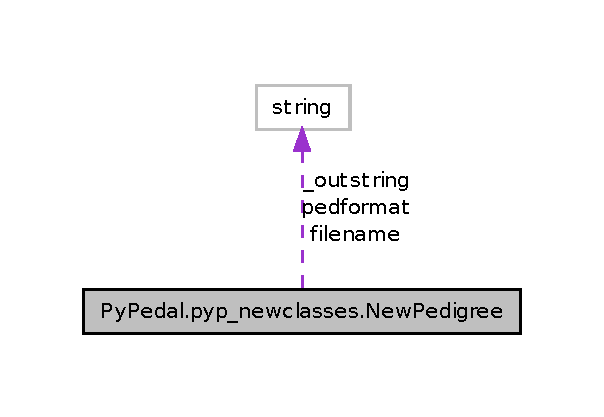
\includegraphics[width=290pt]{classPyPedal_1_1pyp__newclasses_1_1NewPedigree__coll__graph}
\end{center}
\end{figure}
\subsection*{Public Member Functions}
\begin{DoxyCompactItemize}
\item 
def \hyperlink{classPyPedal_1_1pyp__newclasses_1_1NewPedigree_ad6a2650eb959399a93d9c445b53a5b10}{\_\-\_\-init\_\-\_\-}
\begin{DoxyCompactList}\small\item\em \hyperlink{classPyPedal_1_1pyp__newclasses_1_1NewPedigree_ad6a2650eb959399a93d9c445b53a5b10}{\_\-\_\-init\_\-\_\-()} initializes a \hyperlink{classPyPedal_1_1pyp__newclasses_1_1NewPedigree}{NewPedigree} object. \item\end{DoxyCompactList}\item 
def \hyperlink{classPyPedal_1_1pyp__newclasses_1_1NewPedigree_a6f00326b1b20146f6c7ac15596a58448}{load}
\begin{DoxyCompactList}\small\item\em \hyperlink{classPyPedal_1_1pyp__newclasses_1_1NewPedigree_a6f00326b1b20146f6c7ac15596a58448}{load()} wraps several processes useful for loading and preparing a pedigree for use in an analysis, including reading the animals into a list of animal objects, forming lists of sires and dams, checking for common errors, setting ancestor flags, and renumbering the pedigree. \item\end{DoxyCompactList}\item 
def \hyperlink{classPyPedal_1_1pyp__newclasses_1_1NewPedigree_ab7599a24c35efdfcd2caacae10f59ea2}{oldsave}
\begin{DoxyCompactList}\small\item\em \hyperlink{classPyPedal_1_1pyp__newclasses_1_1NewPedigree_ab7599a24c35efdfcd2caacae10f59ea2}{oldsave()} writes a PyPedal pedigree to a user-\/specified file. \item\end{DoxyCompactList}\item 
def \hyperlink{classPyPedal_1_1pyp__newclasses_1_1NewPedigree_ab2c07236058bb89d5318a7453cb6db29}{save}
\begin{DoxyCompactList}\small\item\em \hyperlink{classPyPedal_1_1pyp__newclasses_1_1NewPedigree_ab2c07236058bb89d5318a7453cb6db29}{save()} writes a PyPedal pedigree to a user-\/specified file. \item\end{DoxyCompactList}\item 
def \hyperlink{classPyPedal_1_1pyp__newclasses_1_1NewPedigree_a6babcd0407dd75ff3e5351c96da085aa}{savegraph}
\begin{DoxyCompactList}\small\item\em \hyperlink{classPyPedal_1_1pyp__newclasses_1_1NewPedigree_a6babcd0407dd75ff3e5351c96da085aa}{savegraph()} save a pedigree to a file as an adjacency list. \item\end{DoxyCompactList}\item 
def \hyperlink{classPyPedal_1_1pyp__newclasses_1_1NewPedigree_a4f3ef3055fd807086da58aac2c6499f7}{savegedcom}
\begin{DoxyCompactList}\small\item\em \hyperlink{classPyPedal_1_1pyp__newclasses_1_1NewPedigree_a4f3ef3055fd807086da58aac2c6499f7}{savegedcom()} save a pedigree to a file in GEDCOM 5.5 format. \item\end{DoxyCompactList}\item 
def \hyperlink{classPyPedal_1_1pyp__newclasses_1_1NewPedigree_a41abde8769a72486d5d0e352072338d4}{savegenes}
\begin{DoxyCompactList}\small\item\em \hyperlink{classPyPedal_1_1pyp__newclasses_1_1NewPedigree_a41abde8769a72486d5d0e352072338d4}{savegenes()} save a pedigree to a file in GENES 1.20 (dBase III) format. \item\end{DoxyCompactList}\item 
def \hyperlink{classPyPedal_1_1pyp__newclasses_1_1NewPedigree_abe7890df1b04734981aa7e1e1e4054ec}{savedb}
\begin{DoxyCompactList}\small\item\em \hyperlink{classPyPedal_1_1pyp__newclasses_1_1NewPedigree_abe7890df1b04734981aa7e1e1e4054ec}{savedb()} saves a pedigree to a database table in ASDx format for NewAnimals and LightAnimals. \item\end{DoxyCompactList}\item 
def \hyperlink{classPyPedal_1_1pyp__newclasses_1_1NewPedigree_aa70701de178f69d9c7a3321448681a03}{preprocess}
\begin{DoxyCompactList}\small\item\em \hyperlink{classPyPedal_1_1pyp__newclasses_1_1NewPedigree_aa70701de178f69d9c7a3321448681a03}{preprocess()} processes a pedigree file, which includes reading the animals into a list of animal objects, forming lists of sires and dams, and checking for common errors. \item\end{DoxyCompactList}\item 
def \hyperlink{classPyPedal_1_1pyp__newclasses_1_1NewPedigree_a9d014c1ead82bb6abe3085058086194a}{fromgraph}
\begin{DoxyCompactList}\small\item\em \hyperlink{classPyPedal_1_1pyp__newclasses_1_1NewPedigree_a9d014c1ead82bb6abe3085058086194a}{fromgraph()} loads the animals to populate the pedigree from a DiGraph object. \item\end{DoxyCompactList}\item 
def \hyperlink{classPyPedal_1_1pyp__newclasses_1_1NewPedigree_a7b8f4dca3f231f6d487fee90e38e21c7}{tostream}
\begin{DoxyCompactList}\small\item\em \hyperlink{classPyPedal_1_1pyp__newclasses_1_1NewPedigree_a7b8f4dca3f231f6d487fee90e38e21c7}{tostream()} creates a text stream from a pedigree. \item\end{DoxyCompactList}\item 
def \hyperlink{classPyPedal_1_1pyp__newclasses_1_1NewPedigree_aef198ff1c3c2ac1c666486deb2d2e92a}{renumber}
\begin{DoxyCompactList}\small\item\em \hyperlink{classPyPedal_1_1pyp__newclasses_1_1NewPedigree_aef198ff1c3c2ac1c666486deb2d2e92a}{renumber()} updates the ID map after a pedigree has been renumbered so that all references are to renumbered rather than original IDs. \item\end{DoxyCompactList}\item 
def \hyperlink{classPyPedal_1_1pyp__newclasses_1_1NewPedigree_a6537e2f0a419e0736b500c560b9f6194}{addanimal}
\begin{DoxyCompactList}\small\item\em \hyperlink{classPyPedal_1_1pyp__newclasses_1_1NewPedigree_a6537e2f0a419e0736b500c560b9f6194}{addanimal()} adds a new animal of class \hyperlink{classPyPedal_1_1pyp__newclasses_1_1NewAnimal}{NewAnimal} to the pedigree. \item\end{DoxyCompactList}\item 
def \hyperlink{classPyPedal_1_1pyp__newclasses_1_1NewPedigree_a646940eb2010d378c761e3c8c0e584e6}{delanimal}
\begin{DoxyCompactList}\small\item\em \hyperlink{classPyPedal_1_1pyp__newclasses_1_1NewPedigree_a646940eb2010d378c761e3c8c0e584e6}{delanimal()} deletes an animal from the pedigree. \item\end{DoxyCompactList}\item 
def \hyperlink{classPyPedal_1_1pyp__newclasses_1_1NewPedigree_a5f2e95dd43e8bf2b4bfa2907eebd62a1}{updateidmap}
\begin{DoxyCompactList}\small\item\em \hyperlink{classPyPedal_1_1pyp__newclasses_1_1NewPedigree_a5f2e95dd43e8bf2b4bfa2907eebd62a1}{updateidmap()} updates the ID map after a pedigree has been renumbered so that all references are to renumbered rather than original IDs. \item\end{DoxyCompactList}\item 
def \hyperlink{classPyPedal_1_1pyp__newclasses_1_1NewPedigree_ade3f012ba187d2a311e8e85b82167a3f}{printoptions}
\begin{DoxyCompactList}\small\item\em \hyperlink{classPyPedal_1_1pyp__newclasses_1_1NewPedigree_ade3f012ba187d2a311e8e85b82167a3f}{printoptions()} prints the contents of the options dictionary. \item\end{DoxyCompactList}\item 
def \hyperlink{classPyPedal_1_1pyp__newclasses_1_1NewPedigree_a1d239866c3dacb51ad925bbdf9337001}{simulate}
\begin{DoxyCompactList}\small\item\em \hyperlink{classPyPedal_1_1pyp__newclasses_1_1NewPedigree_a1d239866c3dacb51ad925bbdf9337001}{simulate()} simulates an arbitrary pedigree of size n with g generations starting from n\_\-s base sires and n\_\-d base dams. \item\end{DoxyCompactList}\end{DoxyCompactItemize}
\subsection*{Public Attributes}
\begin{DoxyCompactItemize}
\item 
\hypertarget{classPyPedal_1_1pyp__newclasses_1_1NewPedigree_a28eed1e3039de3a74d2597d556ac831f}{
{\bfseries pedigree}}
\label{classPyPedal_1_1pyp__newclasses_1_1NewPedigree_a28eed1e3039de3a74d2597d556ac831f}

\item 
\hypertarget{classPyPedal_1_1pyp__newclasses_1_1NewPedigree_aae0a246b4cad4a16fc6179a1b1c7548e}{
{\bfseries nrm}}
\label{classPyPedal_1_1pyp__newclasses_1_1NewPedigree_aae0a246b4cad4a16fc6179a1b1c7548e}

\item 
\hypertarget{classPyPedal_1_1pyp__newclasses_1_1NewPedigree_a607a73425bb9710fe4ca7f47f1ffc0fd}{
{\bfseries metadata}}
\label{classPyPedal_1_1pyp__newclasses_1_1NewPedigree_a607a73425bb9710fe4ca7f47f1ffc0fd}

\item 
\hypertarget{classPyPedal_1_1pyp__newclasses_1_1NewPedigree_aab4ab96d9bbce43c2d7c09977bd82d9a}{
{\bfseries namemap}}
\label{classPyPedal_1_1pyp__newclasses_1_1NewPedigree_aab4ab96d9bbce43c2d7c09977bd82d9a}

\item 
\hypertarget{classPyPedal_1_1pyp__newclasses_1_1NewPedigree_adb79d76cbccbc5c03edc64c116f3f43a}{
{\bfseries namebackmap}}
\label{classPyPedal_1_1pyp__newclasses_1_1NewPedigree_adb79d76cbccbc5c03edc64c116f3f43a}

\item 
\hypertarget{classPyPedal_1_1pyp__newclasses_1_1NewPedigree_ae1358ecde62705c1e68fef7a1d943d7e}{
{\bfseries idmap}}
\label{classPyPedal_1_1pyp__newclasses_1_1NewPedigree_ae1358ecde62705c1e68fef7a1d943d7e}

\item 
\hypertarget{classPyPedal_1_1pyp__newclasses_1_1NewPedigree_a6b8ebfe1128f217497e0604e450066db}{
{\bfseries backmap}}
\label{classPyPedal_1_1pyp__newclasses_1_1NewPedigree_a6b8ebfe1128f217497e0604e450066db}

\end{DoxyCompactItemize}
\subsection*{Static Public Attributes}
\begin{DoxyCompactItemize}
\item 
\hypertarget{classPyPedal_1_1pyp__newclasses_1_1NewPedigree_a77c219cbbdbde1d31ae5fee662698c5b}{
tuple {\bfseries pedformat\_\-in} = str(pedformat)}
\label{classPyPedal_1_1pyp__newclasses_1_1NewPedigree_a77c219cbbdbde1d31ae5fee662698c5b}

\item 
\hypertarget{classPyPedal_1_1pyp__newclasses_1_1NewPedigree_a09f9e630dcc8b1c1f5082deb9ec5c377}{
string {\bfseries pedformat} = ''}
\label{classPyPedal_1_1pyp__newclasses_1_1NewPedigree_a09f9e630dcc8b1c1f5082deb9ec5c377}

\item 
\hypertarget{classPyPedal_1_1pyp__newclasses_1_1NewPedigree_a95d6943300b12758ebc4074eaf2154ce}{
list {\bfseries sepchar} = self.kw\mbox{[}'sepchar'\mbox{]}}
\label{classPyPedal_1_1pyp__newclasses_1_1NewPedigree_a95d6943300b12758ebc4074eaf2154ce}

\item 
\hypertarget{classPyPedal_1_1pyp__newclasses_1_1NewPedigree_a82a4ea979cfd080ad108bb9ad20e1215}{
string {\bfseries filename} = '\%s\_\-saved.ped'}
\label{classPyPedal_1_1pyp__newclasses_1_1NewPedigree_a82a4ea979cfd080ad108bb9ad20e1215}

\item 
\hypertarget{classPyPedal_1_1pyp__newclasses_1_1NewPedigree_a45ee1c369ae5e31ebcbc4ac69de4286e}{
tuple {\bfseries ofh} = file(filename,'w')}
\label{classPyPedal_1_1pyp__newclasses_1_1NewPedigree_a45ee1c369ae5e31ebcbc4ac69de4286e}

\item 
\hypertarget{classPyPedal_1_1pyp__newclasses_1_1NewPedigree_a4fc90a3db622e90771d674597da1cccf}{
tuple {\bfseries value} = getattr(\_\-a, self.new\_\-animal\_\-attr\mbox{[}pf\mbox{]})}
\label{classPyPedal_1_1pyp__newclasses_1_1NewPedigree_a4fc90a3db622e90771d674597da1cccf}

\end{DoxyCompactItemize}


\subsection{Detailed Description}
The \hyperlink{classPyPedal_1_1pyp__newclasses_1_1NewPedigree}{NewPedigree} class is the main data structure for PyP 2.0.0Final. 

Definition at line 39 of file pyp\_\-newclasses.py.



\subsection{Member Function Documentation}
\hypertarget{classPyPedal_1_1pyp__newclasses_1_1NewPedigree_ad6a2650eb959399a93d9c445b53a5b10}{
\index{PyPedal::pyp\_\-newclasses::NewPedigree@{PyPedal::pyp\_\-newclasses::NewPedigree}!\_\-\_\-init\_\-\_\-@{\_\-\_\-init\_\-\_\-}}
\index{\_\-\_\-init\_\-\_\-@{\_\-\_\-init\_\-\_\-}!PyPedal::pyp_newclasses::NewPedigree@{PyPedal::pyp\_\-newclasses::NewPedigree}}
\subsubsection[{\_\-\_\-init\_\-\_\-}]{\setlength{\rightskip}{0pt plus 5cm}def PyPedal.pyp\_\-newclasses.NewPedigree.\_\-\_\-init\_\-\_\- (
\begin{DoxyParamCaption}
\item[{}]{ self, }
\item[{}]{ kw = {\ttfamily \{\}}, }
\item[{}]{ kwfile = {\ttfamily 'pypedal.ini'}}
\end{DoxyParamCaption}
)}}
\label{classPyPedal_1_1pyp__newclasses_1_1NewPedigree_ad6a2650eb959399a93d9c445b53a5b10}


\hyperlink{classPyPedal_1_1pyp__newclasses_1_1NewPedigree_ad6a2650eb959399a93d9c445b53a5b10}{\_\-\_\-init\_\-\_\-()} initializes a \hyperlink{classPyPedal_1_1pyp__newclasses_1_1NewPedigree}{NewPedigree} object. 


\begin{DoxyParams}{Parameters}
\item[{\em self}]Reference to the current NewPedigree() object \item[{\em kw}]A dictionary of options. \item[{\em kwfile}]An optionsl configuration file name \end{DoxyParams}

\begin{DoxyRetVals}{Return values}
\item[{\em An}]instance of a NewPedigree() object \begin{DoxyVerb}
__init__() initializes a NewPedigree object.
\end{DoxyVerb}
 \end{DoxyRetVals}


Definition at line 46 of file pyp\_\-newclasses.py.

\hypertarget{classPyPedal_1_1pyp__newclasses_1_1NewPedigree_a6537e2f0a419e0736b500c560b9f6194}{
\index{PyPedal::pyp\_\-newclasses::NewPedigree@{PyPedal::pyp\_\-newclasses::NewPedigree}!addanimal@{addanimal}}
\index{addanimal@{addanimal}!PyPedal::pyp_newclasses::NewPedigree@{PyPedal::pyp\_\-newclasses::NewPedigree}}
\subsubsection[{addanimal}]{\setlength{\rightskip}{0pt plus 5cm}def PyPedal.pyp\_\-newclasses.NewPedigree.addanimal (
\begin{DoxyParamCaption}
\item[{}]{ self, }
\item[{}]{ animalID, }
\item[{}]{ sireID, }
\item[{}]{ damID}
\end{DoxyParamCaption}
)}}
\label{classPyPedal_1_1pyp__newclasses_1_1NewPedigree_a6537e2f0a419e0736b500c560b9f6194}


\hyperlink{classPyPedal_1_1pyp__newclasses_1_1NewPedigree_a6537e2f0a419e0736b500c560b9f6194}{addanimal()} adds a new animal of class \hyperlink{classPyPedal_1_1pyp__newclasses_1_1NewAnimal}{NewAnimal} to the pedigree. 


\begin{DoxyParams}{Parameters}
\item[{\em self}]Reference to current object. \item[{\em animalID}]ID of the new animal to be added to the pedigree. \item[{\em sireID}]Sire ID of the new animal to be added to the pedigree. \item[{\em damID}]Dam ID of the new animal to be added to the pedigree. \end{DoxyParams}

\begin{DoxyRetVals}{Return values}
\item[{\em 1}]on success, 0 on failure \end{DoxyRetVals}


Definition at line 1327 of file pyp\_\-newclasses.py.

\hypertarget{classPyPedal_1_1pyp__newclasses_1_1NewPedigree_a646940eb2010d378c761e3c8c0e584e6}{
\index{PyPedal::pyp\_\-newclasses::NewPedigree@{PyPedal::pyp\_\-newclasses::NewPedigree}!delanimal@{delanimal}}
\index{delanimal@{delanimal}!PyPedal::pyp_newclasses::NewPedigree@{PyPedal::pyp\_\-newclasses::NewPedigree}}
\subsubsection[{delanimal}]{\setlength{\rightskip}{0pt plus 5cm}def PyPedal.pyp\_\-newclasses.NewPedigree.delanimal (
\begin{DoxyParamCaption}
\item[{}]{ self, }
\item[{}]{ animalID}
\end{DoxyParamCaption}
)}}
\label{classPyPedal_1_1pyp__newclasses_1_1NewPedigree_a646940eb2010d378c761e3c8c0e584e6}


\hyperlink{classPyPedal_1_1pyp__newclasses_1_1NewPedigree_a646940eb2010d378c761e3c8c0e584e6}{delanimal()} deletes an animal from the pedigree. 

Note that this method DOES not update the metadata attached to the pedigree and should only be used if that is not important. As of 04/10/2006 \hyperlink{classPyPedal_1_1pyp__newclasses_1_1NewPedigree_a646940eb2010d378c761e3c8c0e584e6}{delanimal()} is intended for use by pyp\_\-metrics/mating\_\-coi() rather than directly by users. 
\begin{DoxyParams}{Parameters}
\item[{\em self}]Reference to current object \item[{\em animalID}]ID of the animal to be deleted \end{DoxyParams}

\begin{DoxyRetVals}{Return values}
\item[{\em 1}]on success, 0 on failure \end{DoxyRetVals}


Definition at line 1403 of file pyp\_\-newclasses.py.

\hypertarget{classPyPedal_1_1pyp__newclasses_1_1NewPedigree_a9d014c1ead82bb6abe3085058086194a}{
\index{PyPedal::pyp\_\-newclasses::NewPedigree@{PyPedal::pyp\_\-newclasses::NewPedigree}!fromgraph@{fromgraph}}
\index{fromgraph@{fromgraph}!PyPedal::pyp_newclasses::NewPedigree@{PyPedal::pyp\_\-newclasses::NewPedigree}}
\subsubsection[{fromgraph}]{\setlength{\rightskip}{0pt plus 5cm}def PyPedal.pyp\_\-newclasses.NewPedigree.fromgraph (
\begin{DoxyParamCaption}
\item[{}]{ self, }
\item[{}]{ pedgraph}
\end{DoxyParamCaption}
)}}
\label{classPyPedal_1_1pyp__newclasses_1_1NewPedigree_a9d014c1ead82bb6abe3085058086194a}


\hyperlink{classPyPedal_1_1pyp__newclasses_1_1NewPedigree_a9d014c1ead82bb6abe3085058086194a}{fromgraph()} loads the animals to populate the pedigree from a DiGraph object. 


\begin{DoxyParams}{Parameters}
\item[{\em self}]Reference to current object. \item[{\em pedgraph}]DiGraph object containing a pedigree. \end{DoxyParams}

\begin{DoxyRetVals}{Return values}
\item[{\em None}]\begin{DoxyVerb}
fromgraph() loads the animals to populate the pedigree from an
DiGraph object.
\end{DoxyVerb}
 \end{DoxyRetVals}


Definition at line 1228 of file pyp\_\-newclasses.py.

\hypertarget{classPyPedal_1_1pyp__newclasses_1_1NewPedigree_a6f00326b1b20146f6c7ac15596a58448}{
\index{PyPedal::pyp\_\-newclasses::NewPedigree@{PyPedal::pyp\_\-newclasses::NewPedigree}!load@{load}}
\index{load@{load}!PyPedal::pyp_newclasses::NewPedigree@{PyPedal::pyp\_\-newclasses::NewPedigree}}
\subsubsection[{load}]{\setlength{\rightskip}{0pt plus 5cm}def PyPedal.pyp\_\-newclasses.NewPedigree.load (
\begin{DoxyParamCaption}
\item[{}]{ self, }
\item[{}]{ pedsource = {\ttfamily 'file'}, }
\item[{}]{ pedgraph = {\ttfamily 0}, }
\item[{}]{ pedstream = {\ttfamily ''}}
\end{DoxyParamCaption}
)}}
\label{classPyPedal_1_1pyp__newclasses_1_1NewPedigree_a6f00326b1b20146f6c7ac15596a58448}


\hyperlink{classPyPedal_1_1pyp__newclasses_1_1NewPedigree_a6f00326b1b20146f6c7ac15596a58448}{load()} wraps several processes useful for loading and preparing a pedigree for use in an analysis, including reading the animals into a list of animal objects, forming lists of sires and dams, checking for common errors, setting ancestor flags, and renumbering the pedigree. 


\begin{DoxyParams}{Parameters}
\item[{\em self}]Reference to current object. \item[{\em pedsource}]Source of the pedigree ('file'$|$'graph'$|$'graphfile'$|$'db'). \item[{\em pedgraph}]DiGraph from which to load the pedigree. \item[{\em pedstream}]Stream of text from which to load the pedigree. \end{DoxyParams}

\begin{DoxyRetVals}{Return values}
\item[{\em None}]\begin{DoxyVerb}
load() wraps several processes useful for loading and preparing a pedigree for
use in an analysis, including reading the animals into a list of animal objects,
forming lists of sires and dams, checking for common errors, setting ancestor
flags, and renumbering the pedigree.
\end{DoxyVerb}
 \end{DoxyRetVals}


Definition at line 273 of file pyp\_\-newclasses.py.

\hypertarget{classPyPedal_1_1pyp__newclasses_1_1NewPedigree_ab7599a24c35efdfcd2caacae10f59ea2}{
\index{PyPedal::pyp\_\-newclasses::NewPedigree@{PyPedal::pyp\_\-newclasses::NewPedigree}!oldsave@{oldsave}}
\index{oldsave@{oldsave}!PyPedal::pyp_newclasses::NewPedigree@{PyPedal::pyp\_\-newclasses::NewPedigree}}
\subsubsection[{oldsave}]{\setlength{\rightskip}{0pt plus 5cm}def PyPedal.pyp\_\-newclasses.NewPedigree.oldsave (
\begin{DoxyParamCaption}
\item[{}]{ self, }
\item[{}]{ filename = {\ttfamily ''}, }
\item[{}]{ outformat = {\ttfamily 'o'}, }
\item[{}]{ idformat = {\ttfamily 'o'}}
\end{DoxyParamCaption}
)}}
\label{classPyPedal_1_1pyp__newclasses_1_1NewPedigree_ab7599a24c35efdfcd2caacae10f59ea2}


\hyperlink{classPyPedal_1_1pyp__newclasses_1_1NewPedigree_ab7599a24c35efdfcd2caacae10f59ea2}{oldsave()} writes a PyPedal pedigree to a user-\/specified file. 

The saved pedigree includes all fields recognized by PyPedal, not just the original fields read from the input pedigree file. 
\begin{DoxyParams}{Parameters}
\item[{\em self}]Reference to current object. \item[{\em filename}]The file to which the pedigree should be written. \item[{\em outformat}]The format in which the pedigree should be written: 'o' for original (as read) and 'l' for long version (all available variables). \item[{\em idformat}]Write 'o' (original) or 'r' (renumbered) animal, sire, and dam IDs. \end{DoxyParams}

\begin{DoxyRetVals}{Return values}
\item[{\em A}]save status indicator (0: failed, 1: success) \begin{DoxyVerb}
oldsave() writes a PyPedal pedigree to a user-specified file.  The saved pedigree
includes all fields recognized by PyPedal, not just the original fields read
from the input pedigree file.
\end{DoxyVerb}
 \end{DoxyRetVals}


Definition at line 510 of file pyp\_\-newclasses.py.

\hypertarget{classPyPedal_1_1pyp__newclasses_1_1NewPedigree_aa70701de178f69d9c7a3321448681a03}{
\index{PyPedal::pyp\_\-newclasses::NewPedigree@{PyPedal::pyp\_\-newclasses::NewPedigree}!preprocess@{preprocess}}
\index{preprocess@{preprocess}!PyPedal::pyp_newclasses::NewPedigree@{PyPedal::pyp\_\-newclasses::NewPedigree}}
\subsubsection[{preprocess}]{\setlength{\rightskip}{0pt plus 5cm}def PyPedal.pyp\_\-newclasses.NewPedigree.preprocess (
\begin{DoxyParamCaption}
\item[{}]{ self, }
\item[{}]{ textstream = {\ttfamily ''}, }
\item[{}]{ dbstream = {\ttfamily ''}}
\end{DoxyParamCaption}
)}}
\label{classPyPedal_1_1pyp__newclasses_1_1NewPedigree_aa70701de178f69d9c7a3321448681a03}


\hyperlink{classPyPedal_1_1pyp__newclasses_1_1NewPedigree_aa70701de178f69d9c7a3321448681a03}{preprocess()} processes a pedigree file, which includes reading the animals into a list of animal objects, forming lists of sires and dams, and checking for common errors. 


\begin{DoxyParams}{Parameters}
\item[{\em self}]Reference to current object \item[{\em textstream}]String containing animal records \item[{\em dbstream}]List of tuples of animal records \end{DoxyParams}

\begin{DoxyRetVals}{Return values}
\item[{\em None}]\begin{DoxyVerb}
Preprocess a pedigree file, which includes reading the animals into a list, forming lists of sires and dams, and checking for common errors.
\end{DoxyVerb}
 \end{DoxyRetVals}


Definition at line 831 of file pyp\_\-newclasses.py.

\hypertarget{classPyPedal_1_1pyp__newclasses_1_1NewPedigree_ade3f012ba187d2a311e8e85b82167a3f}{
\index{PyPedal::pyp\_\-newclasses::NewPedigree@{PyPedal::pyp\_\-newclasses::NewPedigree}!printoptions@{printoptions}}
\index{printoptions@{printoptions}!PyPedal::pyp_newclasses::NewPedigree@{PyPedal::pyp\_\-newclasses::NewPedigree}}
\subsubsection[{printoptions}]{\setlength{\rightskip}{0pt plus 5cm}def PyPedal.pyp\_\-newclasses.NewPedigree.printoptions (
\begin{DoxyParamCaption}
\item[{}]{ self}
\end{DoxyParamCaption}
)}}
\label{classPyPedal_1_1pyp__newclasses_1_1NewPedigree_ade3f012ba187d2a311e8e85b82167a3f}


\hyperlink{classPyPedal_1_1pyp__newclasses_1_1NewPedigree_ade3f012ba187d2a311e8e85b82167a3f}{printoptions()} prints the contents of the options dictionary. 


\begin{DoxyParams}{Parameters}
\item[{\em self}]Reference to current object \end{DoxyParams}

\begin{DoxyRetVals}{Return values}
\item[{\em None}]\begin{DoxyVerb}
printoptions() prints the contents of the options dictionary.
\end{DoxyVerb}
 \end{DoxyRetVals}


Definition at line 1456 of file pyp\_\-newclasses.py.

\hypertarget{classPyPedal_1_1pyp__newclasses_1_1NewPedigree_aef198ff1c3c2ac1c666486deb2d2e92a}{
\index{PyPedal::pyp\_\-newclasses::NewPedigree@{PyPedal::pyp\_\-newclasses::NewPedigree}!renumber@{renumber}}
\index{renumber@{renumber}!PyPedal::pyp_newclasses::NewPedigree@{PyPedal::pyp\_\-newclasses::NewPedigree}}
\subsubsection[{renumber}]{\setlength{\rightskip}{0pt plus 5cm}def PyPedal.pyp\_\-newclasses.NewPedigree.renumber (
\begin{DoxyParamCaption}
\item[{}]{ self}
\end{DoxyParamCaption}
)}}
\label{classPyPedal_1_1pyp__newclasses_1_1NewPedigree_aef198ff1c3c2ac1c666486deb2d2e92a}


\hyperlink{classPyPedal_1_1pyp__newclasses_1_1NewPedigree_aef198ff1c3c2ac1c666486deb2d2e92a}{renumber()} updates the ID map after a pedigree has been renumbered so that all references are to renumbered rather than original IDs. 


\begin{DoxyParams}{Parameters}
\item[{\em self}]Reference to current object \end{DoxyParams}

\begin{DoxyRetVals}{Return values}
\item[{\em None}]\begin{DoxyVerb}
renumber() updates the ID map after a pedigree has been renumbered so that all
references are to renumbered rather than original IDs.
\end{DoxyVerb}
 \end{DoxyRetVals}


Definition at line 1290 of file pyp\_\-newclasses.py.

\hypertarget{classPyPedal_1_1pyp__newclasses_1_1NewPedigree_ab2c07236058bb89d5318a7453cb6db29}{
\index{PyPedal::pyp\_\-newclasses::NewPedigree@{PyPedal::pyp\_\-newclasses::NewPedigree}!save@{save}}
\index{save@{save}!PyPedal::pyp_newclasses::NewPedigree@{PyPedal::pyp\_\-newclasses::NewPedigree}}
\subsubsection[{save}]{\setlength{\rightskip}{0pt plus 5cm}def PyPedal.pyp\_\-newclasses.NewPedigree.save (
\begin{DoxyParamCaption}
\item[{}]{ self, }
\item[{}]{ filename = {\ttfamily ''}, }
\item[{}]{ pedformat = {\ttfamily 'asd'}, }
\item[{}]{ sepchar = {\ttfamily '~'}}
\end{DoxyParamCaption}
)}}
\label{classPyPedal_1_1pyp__newclasses_1_1NewPedigree_ab2c07236058bb89d5318a7453cb6db29}


\hyperlink{classPyPedal_1_1pyp__newclasses_1_1NewPedigree_ab2c07236058bb89d5318a7453cb6db29}{save()} writes a PyPedal pedigree to a user-\/specified file. 

The saved pedigree includes all fields recognized by PyPedal, not just the original fields read from the input pedigree file. 
\begin{DoxyParams}{Parameters}
\item[{\em self}]Reference to current object. \item[{\em filename}]The file to which the pedigree should be written. \item[{\em pedformat}]Pedigree format string for the pedigree to be written. \item[{\em sepchar}]Character used to separate columns in the output pedigree file. \end{DoxyParams}

\begin{DoxyRetVals}{Return values}
\item[{\em A}]save status indicator (0: failed, 1: success) \begin{DoxyVerb}
save() writes a PyPedal pedigree to a user-specified file.  The saved pedigree
includes all fields recognized by PyPedal, not just the original fields read
from the input pedigree file.
\end{DoxyVerb}
 \end{DoxyRetVals}


Definition at line 611 of file pyp\_\-newclasses.py.

\hypertarget{classPyPedal_1_1pyp__newclasses_1_1NewPedigree_abe7890df1b04734981aa7e1e1e4054ec}{
\index{PyPedal::pyp\_\-newclasses::NewPedigree@{PyPedal::pyp\_\-newclasses::NewPedigree}!savedb@{savedb}}
\index{savedb@{savedb}!PyPedal::pyp_newclasses::NewPedigree@{PyPedal::pyp\_\-newclasses::NewPedigree}}
\subsubsection[{savedb}]{\setlength{\rightskip}{0pt plus 5cm}def PyPedal.pyp\_\-newclasses.NewPedigree.savedb (
\begin{DoxyParamCaption}
\item[{}]{ self, }
\item[{}]{ drop = {\ttfamily False}}
\end{DoxyParamCaption}
)}}
\label{classPyPedal_1_1pyp__newclasses_1_1NewPedigree_abe7890df1b04734981aa7e1e1e4054ec}


\hyperlink{classPyPedal_1_1pyp__newclasses_1_1NewPedigree_abe7890df1b04734981aa7e1e1e4054ec}{savedb()} saves a pedigree to a database table in ASDx format for NewAnimals and LightAnimals. 


\begin{DoxyParams}{Parameters}
\item[{\em self}]Reference to current object. \item[{\em drop}]Boolean indicating if existing data should be kept (False) or deleted (True); the default is False. \end{DoxyParams}

\begin{DoxyRetVals}{Return values}
\item[{\em \_\-savedb\_\-status}]Boolean indicating if the pedigree was successfully saved. \begin{DoxyVerb}
savedb() saves a pedigree to a database table in ASDx format
for NewAnimals and LightAnimals.
\end{DoxyVerb}
 \end{DoxyRetVals}


Definition at line 757 of file pyp\_\-newclasses.py.

\hypertarget{classPyPedal_1_1pyp__newclasses_1_1NewPedigree_a4f3ef3055fd807086da58aac2c6499f7}{
\index{PyPedal::pyp\_\-newclasses::NewPedigree@{PyPedal::pyp\_\-newclasses::NewPedigree}!savegedcom@{savegedcom}}
\index{savegedcom@{savegedcom}!PyPedal::pyp_newclasses::NewPedigree@{PyPedal::pyp\_\-newclasses::NewPedigree}}
\subsubsection[{savegedcom}]{\setlength{\rightskip}{0pt plus 5cm}def PyPedal.pyp\_\-newclasses.NewPedigree.savegedcom (
\begin{DoxyParamCaption}
\item[{}]{ self, }
\item[{}]{ pedoutfile = {\ttfamily 0}}
\end{DoxyParamCaption}
)}}
\label{classPyPedal_1_1pyp__newclasses_1_1NewPedigree_a4f3ef3055fd807086da58aac2c6499f7}


\hyperlink{classPyPedal_1_1pyp__newclasses_1_1NewPedigree_a4f3ef3055fd807086da58aac2c6499f7}{savegedcom()} save a pedigree to a file in GEDCOM 5.5 format. 


\begin{DoxyParams}{Parameters}
\item[{\em self}]Reference to current object \item[{\em pedoutfile}]Name of the file to which the graph is written \end{DoxyParams}

\begin{DoxyRetVals}{Return values}
\item[{\em None}]\begin{DoxyVerb}
Save a pedigree to a file in GEDCOM 5.5 format.
\end{DoxyVerb}
 \end{DoxyRetVals}


Definition at line 722 of file pyp\_\-newclasses.py.

\hypertarget{classPyPedal_1_1pyp__newclasses_1_1NewPedigree_a41abde8769a72486d5d0e352072338d4}{
\index{PyPedal::pyp\_\-newclasses::NewPedigree@{PyPedal::pyp\_\-newclasses::NewPedigree}!savegenes@{savegenes}}
\index{savegenes@{savegenes}!PyPedal::pyp_newclasses::NewPedigree@{PyPedal::pyp\_\-newclasses::NewPedigree}}
\subsubsection[{savegenes}]{\setlength{\rightskip}{0pt plus 5cm}def PyPedal.pyp\_\-newclasses.NewPedigree.savegenes (
\begin{DoxyParamCaption}
\item[{}]{ self, }
\item[{}]{ pedoutfile = {\ttfamily 0}}
\end{DoxyParamCaption}
)}}
\label{classPyPedal_1_1pyp__newclasses_1_1NewPedigree_a41abde8769a72486d5d0e352072338d4}


\hyperlink{classPyPedal_1_1pyp__newclasses_1_1NewPedigree_a41abde8769a72486d5d0e352072338d4}{savegenes()} save a pedigree to a file in GENES 1.20 (dBase III) format. 


\begin{DoxyParams}{Parameters}
\item[{\em self}]Reference to current object \item[{\em pedoutfile}]Name of the file to which the graph is written \end{DoxyParams}

\begin{DoxyRetVals}{Return values}
\item[{\em None}]\begin{DoxyVerb}
Save a pedigree to a file in GENES 1.20 (dBase III) format.
\end{DoxyVerb}
 \end{DoxyRetVals}


Definition at line 739 of file pyp\_\-newclasses.py.

\hypertarget{classPyPedal_1_1pyp__newclasses_1_1NewPedigree_a6babcd0407dd75ff3e5351c96da085aa}{
\index{PyPedal::pyp\_\-newclasses::NewPedigree@{PyPedal::pyp\_\-newclasses::NewPedigree}!savegraph@{savegraph}}
\index{savegraph@{savegraph}!PyPedal::pyp_newclasses::NewPedigree@{PyPedal::pyp\_\-newclasses::NewPedigree}}
\subsubsection[{savegraph}]{\setlength{\rightskip}{0pt plus 5cm}def PyPedal.pyp\_\-newclasses.NewPedigree.savegraph (
\begin{DoxyParamCaption}
\item[{}]{ self, }
\item[{}]{ pedoutfile = {\ttfamily 0}, }
\item[{}]{ pedgraph = {\ttfamily 0}}
\end{DoxyParamCaption}
)}}
\label{classPyPedal_1_1pyp__newclasses_1_1NewPedigree_a6babcd0407dd75ff3e5351c96da085aa}


\hyperlink{classPyPedal_1_1pyp__newclasses_1_1NewPedigree_a6babcd0407dd75ff3e5351c96da085aa}{savegraph()} save a pedigree to a file as an adjacency list. 


\begin{DoxyParams}{Parameters}
\item[{\em self}]Reference to current object. \item[{\em pedoutfile}]Name of the file to which the graph is written. \item[{\em pedgraph}]Graph object \end{DoxyParams}

\begin{DoxyRetVals}{Return values}
\item[{\em None}]\begin{DoxyVerb}
Save a pedigree to a file as an adjacency list.
\end{DoxyVerb}
 \end{DoxyRetVals}


Definition at line 698 of file pyp\_\-newclasses.py.

\hypertarget{classPyPedal_1_1pyp__newclasses_1_1NewPedigree_a1d239866c3dacb51ad925bbdf9337001}{
\index{PyPedal::pyp\_\-newclasses::NewPedigree@{PyPedal::pyp\_\-newclasses::NewPedigree}!simulate@{simulate}}
\index{simulate@{simulate}!PyPedal::pyp_newclasses::NewPedigree@{PyPedal::pyp\_\-newclasses::NewPedigree}}
\subsubsection[{simulate}]{\setlength{\rightskip}{0pt plus 5cm}def PyPedal.pyp\_\-newclasses.NewPedigree.simulate (
\begin{DoxyParamCaption}
\item[{}]{ self}
\end{DoxyParamCaption}
)}}
\label{classPyPedal_1_1pyp__newclasses_1_1NewPedigree_a1d239866c3dacb51ad925bbdf9337001}


\hyperlink{classPyPedal_1_1pyp__newclasses_1_1NewPedigree_a1d239866c3dacb51ad925bbdf9337001}{simulate()} simulates an arbitrary pedigree of size n with g generations starting from n\_\-s base sires and n\_\-d base dams. 

This method is based on the concepts and algorithms in the Pedigree.sample method from Matvec 1.1a. The arguments are read from the pedigree object's options dictionary. 
\begin{DoxyParams}{Parameters}
\item[{\em self}]Reference to current object \end{DoxyParams}

\begin{DoxyRetVals}{Return values}
\item[{\em None}]\begin{DoxyVerb}
Simulate simulates an arbitrary pedigree of size n with g generations
starting from n_s base sires and n_d base dams.  This method is based
on the concepts and algorithms in the Pedigree::sample method from
Matvec 1.1a (src/classes/pedigree.cpp), although all of the code in
this implementation was written from scratch.
\end{DoxyVerb}
 \end{DoxyRetVals}


Definition at line 1475 of file pyp\_\-newclasses.py.

\hypertarget{classPyPedal_1_1pyp__newclasses_1_1NewPedigree_a7b8f4dca3f231f6d487fee90e38e21c7}{
\index{PyPedal::pyp\_\-newclasses::NewPedigree@{PyPedal::pyp\_\-newclasses::NewPedigree}!tostream@{tostream}}
\index{tostream@{tostream}!PyPedal::pyp_newclasses::NewPedigree@{PyPedal::pyp\_\-newclasses::NewPedigree}}
\subsubsection[{tostream}]{\setlength{\rightskip}{0pt plus 5cm}def PyPedal.pyp\_\-newclasses.NewPedigree.tostream (
\begin{DoxyParamCaption}
\item[{}]{ self}
\end{DoxyParamCaption}
)}}
\label{classPyPedal_1_1pyp__newclasses_1_1NewPedigree_a7b8f4dca3f231f6d487fee90e38e21c7}


\hyperlink{classPyPedal_1_1pyp__newclasses_1_1NewPedigree_a7b8f4dca3f231f6d487fee90e38e21c7}{tostream()} creates a text stream from a pedigree. 


\begin{DoxyParams}{Parameters}
\item[{\em self}]Reference to current object \end{DoxyParams}

\begin{DoxyRetVals}{Return values}
\item[{\em None}]\begin{DoxyVerb}
tostream() creates a text stream from a pedigree.
\end{DoxyVerb}
 \end{DoxyRetVals}


Definition at line 1261 of file pyp\_\-newclasses.py.

\hypertarget{classPyPedal_1_1pyp__newclasses_1_1NewPedigree_a5f2e95dd43e8bf2b4bfa2907eebd62a1}{
\index{PyPedal::pyp\_\-newclasses::NewPedigree@{PyPedal::pyp\_\-newclasses::NewPedigree}!updateidmap@{updateidmap}}
\index{updateidmap@{updateidmap}!PyPedal::pyp_newclasses::NewPedigree@{PyPedal::pyp\_\-newclasses::NewPedigree}}
\subsubsection[{updateidmap}]{\setlength{\rightskip}{0pt plus 5cm}def PyPedal.pyp\_\-newclasses.NewPedigree.updateidmap (
\begin{DoxyParamCaption}
\item[{}]{ self}
\end{DoxyParamCaption}
)}}
\label{classPyPedal_1_1pyp__newclasses_1_1NewPedigree_a5f2e95dd43e8bf2b4bfa2907eebd62a1}


\hyperlink{classPyPedal_1_1pyp__newclasses_1_1NewPedigree_a5f2e95dd43e8bf2b4bfa2907eebd62a1}{updateidmap()} updates the ID map after a pedigree has been renumbered so that all references are to renumbered rather than original IDs. 


\begin{DoxyParams}{Parameters}
\item[{\em self}]Reference to current object \end{DoxyParams}

\begin{DoxyRetVals}{Return values}
\item[{\em None}]\begin{DoxyVerb}
updateidmap() updates the ID map after a pedigree has been renumbered so that
all references are to renumbered rather than original IDs.
\end{DoxyVerb}
 \end{DoxyRetVals}


Definition at line 1424 of file pyp\_\-newclasses.py.



The documentation for this class was generated from the following file:\begin{DoxyCompactItemize}
\item 
PyPedal/pyp\_\-newclasses.py\end{DoxyCompactItemize}

\hypertarget{classPyPedal_1_1pyp__classes_1_1Pedigree}{
\section{PyPedal.pyp\_\-classes.Pedigree Class Reference}
\label{classPyPedal_1_1pyp__classes_1_1Pedigree}\index{PyPedal::pyp\_\-classes::Pedigree@{PyPedal::pyp\_\-classes::Pedigree}}
}


The Pedigree() class stores metadata about pedigrees.  


\subsection*{Public Member Functions}
\begin{DoxyCompactItemize}
\item 
def \hyperlink{classPyPedal_1_1pyp__classes_1_1Pedigree_ade39878cc44e604f0d2f1023a9014518}{\_\-\_\-init\_\-\_\-}
\begin{DoxyCompactList}\small\item\em \hyperlink{classPyPedal_1_1pyp__classes_1_1Pedigree_ade39878cc44e604f0d2f1023a9014518}{\_\-\_\-init\_\-\_\-()} initializes a \hyperlink{classPyPedal_1_1pyp__classes_1_1Pedigree}{Pedigree} metata object. \end{DoxyCompactList}\item 
def \hyperlink{classPyPedal_1_1pyp__classes_1_1Pedigree_ab8c2b67da1b07fedf79d997172b72a03}{printme}
\begin{DoxyCompactList}\small\item\em \hyperlink{classPyPedal_1_1pyp__classes_1_1Pedigree_ab8c2b67da1b07fedf79d997172b72a03}{printme()} prints a summary of the metadata stored in the Pedigree() object. \end{DoxyCompactList}\item 
def \hyperlink{classPyPedal_1_1pyp__classes_1_1Pedigree_ac4a0cad61344517ea9a1b00b6f1ee007}{stringme}
\begin{DoxyCompactList}\small\item\em \hyperlink{classPyPedal_1_1pyp__classes_1_1Pedigree_ac4a0cad61344517ea9a1b00b6f1ee007}{stringme()} returns a summary of the metadata stored in the pedigree as a string. \end{DoxyCompactList}\item 
def \hyperlink{classPyPedal_1_1pyp__classes_1_1Pedigree_a009aa82eb9e76635475f092c269a719f}{fileme}
\begin{DoxyCompactList}\small\item\em \hyperlink{classPyPedal_1_1pyp__classes_1_1Pedigree_a009aa82eb9e76635475f092c269a719f}{fileme()} writes the metada stored in the Pedigree() object to disc. \end{DoxyCompactList}\item 
def \hyperlink{classPyPedal_1_1pyp__classes_1_1Pedigree_ad89f110b30544721eeaa945e50f467ff}{nus}
\begin{DoxyCompactList}\small\item\em \hyperlink{classPyPedal_1_1pyp__classes_1_1Pedigree_ad89f110b30544721eeaa945e50f467ff}{nus()} returns the number of unique sires in the pedigree along with a list of the sires \end{DoxyCompactList}\item 
def \hyperlink{classPyPedal_1_1pyp__classes_1_1Pedigree_a5da0b261e57cab87dd06af5e07aeb55e}{nud}
\begin{DoxyCompactList}\small\item\em \hyperlink{classPyPedal_1_1pyp__classes_1_1Pedigree_a5da0b261e57cab87dd06af5e07aeb55e}{nud()} returns the number of unique dams in the pedigree along with a list of the dams \end{DoxyCompactList}\item 
def \hyperlink{classPyPedal_1_1pyp__classes_1_1Pedigree_acc0248a985179c7c58a41d71b4e11799}{nug}
\begin{DoxyCompactList}\small\item\em \hyperlink{classPyPedal_1_1pyp__classes_1_1Pedigree_acc0248a985179c7c58a41d71b4e11799}{nug()} returns the number of unique generations in the pedigree along with a list of the generations \end{DoxyCompactList}\item 
def \hyperlink{classPyPedal_1_1pyp__classes_1_1Pedigree_a350271baa0007e5c9e0fd5652f29c399}{nuy}
\begin{DoxyCompactList}\small\item\em \hyperlink{classPyPedal_1_1pyp__classes_1_1Pedigree_a350271baa0007e5c9e0fd5652f29c399}{nuy()} returns the number of unique birthyears in the pedigree along with a list of the birthyears \end{DoxyCompactList}\item 
def \hyperlink{classPyPedal_1_1pyp__classes_1_1Pedigree_a3b7ebee81bdb56eb9343795e2faa9611}{nuf}
\begin{DoxyCompactList}\small\item\em \hyperlink{classPyPedal_1_1pyp__classes_1_1Pedigree_a3b7ebee81bdb56eb9343795e2faa9611}{nuf()} returns the number of unique founders in the pedigree along with a list of the founders \end{DoxyCompactList}\end{DoxyCompactItemize}
\subsection*{Public Attributes}
\begin{DoxyCompactItemize}
\item 
\hypertarget{classPyPedal_1_1pyp__classes_1_1Pedigree_ae43d863c0ff07f1c0bd011d4a6b4f1f3}{
{\bfseries name}}
\label{classPyPedal_1_1pyp__classes_1_1Pedigree_ae43d863c0ff07f1c0bd011d4a6b4f1f3}

\item 
\hypertarget{classPyPedal_1_1pyp__classes_1_1Pedigree_a8df29b089491e403e1c95795d27ed975}{
{\bfseries filename}}
\label{classPyPedal_1_1pyp__classes_1_1Pedigree_a8df29b089491e403e1c95795d27ed975}

\item 
\hypertarget{classPyPedal_1_1pyp__classes_1_1Pedigree_a81f67249798fe99971a058421b845a18}{
{\bfseries myped}}
\label{classPyPedal_1_1pyp__classes_1_1Pedigree_a81f67249798fe99971a058421b845a18}

\item 
\hypertarget{classPyPedal_1_1pyp__classes_1_1Pedigree_aaf888dc23bb042fe2c225c14ca484caa}{
{\bfseries pedcode}}
\label{classPyPedal_1_1pyp__classes_1_1Pedigree_aaf888dc23bb042fe2c225c14ca484caa}

\item 
\hypertarget{classPyPedal_1_1pyp__classes_1_1Pedigree_a8443382b5d34d5426e2228e1130c1650}{
{\bfseries num\_\-records}}
\label{classPyPedal_1_1pyp__classes_1_1Pedigree_a8443382b5d34d5426e2228e1130c1650}

\item 
\hypertarget{classPyPedal_1_1pyp__classes_1_1Pedigree_a91cb2a215dbfa1a3f29921c0ebc13f50}{
{\bfseries unique\_\-sire\_\-list}}
\label{classPyPedal_1_1pyp__classes_1_1Pedigree_a91cb2a215dbfa1a3f29921c0ebc13f50}

\item 
\hypertarget{classPyPedal_1_1pyp__classes_1_1Pedigree_a8d57c8f307015154c2d48d076e2590a0}{
{\bfseries unique\_\-dam\_\-list}}
\label{classPyPedal_1_1pyp__classes_1_1Pedigree_a8d57c8f307015154c2d48d076e2590a0}

\item 
\hypertarget{classPyPedal_1_1pyp__classes_1_1Pedigree_ad090a367c837eba7be5497d8c4154bb3}{
{\bfseries reordered}}
\label{classPyPedal_1_1pyp__classes_1_1Pedigree_ad090a367c837eba7be5497d8c4154bb3}

\item 
\hypertarget{classPyPedal_1_1pyp__classes_1_1Pedigree_a6bac64e40a7d50f0586ea3971531edad}{
{\bfseries renumbered}}
\label{classPyPedal_1_1pyp__classes_1_1Pedigree_a6bac64e40a7d50f0586ea3971531edad}

\item 
\hypertarget{classPyPedal_1_1pyp__classes_1_1Pedigree_ad7407edfa4137d35c03a219e7bb6e12f}{
{\bfseries unique\_\-gen\_\-list}}
\label{classPyPedal_1_1pyp__classes_1_1Pedigree_ad7407edfa4137d35c03a219e7bb6e12f}

\item 
\hypertarget{classPyPedal_1_1pyp__classes_1_1Pedigree_a879e092db5cd36a44d60ba96e536346a}{
{\bfseries unique\_\-year\_\-list}}
\label{classPyPedal_1_1pyp__classes_1_1Pedigree_a879e092db5cd36a44d60ba96e536346a}

\item 
\hypertarget{classPyPedal_1_1pyp__classes_1_1Pedigree_a691b90a99107c293d97b6d8611781beb}{
{\bfseries unique\_\-founder\_\-list}}
\label{classPyPedal_1_1pyp__classes_1_1Pedigree_a691b90a99107c293d97b6d8611781beb}

\end{DoxyCompactItemize}


\subsection{Detailed Description}
The Pedigree() class stores metadata about pedigrees. 

Hopefully this will help improve performance in some procedures, as well as provide some useful summary data. \begin{DoxyVerb}A class to hold metadata about pedigrees.  Hopefully this will help improve performance in some procedures, as well as
provide some useful summary data.\end{DoxyVerb}
 

Definition at line 199 of file pyp\_\-classes.py.



\subsection{Constructor \& Destructor Documentation}
\hypertarget{classPyPedal_1_1pyp__classes_1_1Pedigree_ade39878cc44e604f0d2f1023a9014518}{
\index{PyPedal::pyp\_\-classes::Pedigree@{PyPedal::pyp\_\-classes::Pedigree}!\_\-\_\-init\_\-\_\-@{\_\-\_\-init\_\-\_\-}}
\index{\_\-\_\-init\_\-\_\-@{\_\-\_\-init\_\-\_\-}!PyPedal::pyp_classes::Pedigree@{PyPedal::pyp\_\-classes::Pedigree}}
\subsubsection[{\_\-\_\-init\_\-\_\-}]{\setlength{\rightskip}{0pt plus 5cm}def PyPedal.pyp\_\-classes.Pedigree.\_\-\_\-init\_\-\_\- (
\begin{DoxyParamCaption}
\item[{}]{self, }
\item[{}]{myped, }
\item[{}]{inputfile, }
\item[{}]{name, }
\item[{}]{pedcode = {\ttfamily 'asd'}, }
\item[{}]{reord = {\ttfamily 0}, }
\item[{}]{renum = {\ttfamily 0}, }
\item[{}]{debug = {\ttfamily 0}}
\end{DoxyParamCaption}
)}}
\label{classPyPedal_1_1pyp__classes_1_1Pedigree_ade39878cc44e604f0d2f1023a9014518}


\hyperlink{classPyPedal_1_1pyp__classes_1_1Pedigree_ade39878cc44e604f0d2f1023a9014518}{\_\-\_\-init\_\-\_\-()} initializes a \hyperlink{classPyPedal_1_1pyp__classes_1_1Pedigree}{Pedigree} metata object. 


\begin{DoxyParams}{Parameters}
{\em self} & Reference to the current Pedigree() object \\
\hline
{\em myped} & A PyPedal pedigree \\
\hline
{\em inputfile} & The name of the file from which the pedigree was loaded \\
\hline
{\em name} & The name assigned to the PyPedal pedigree \\
\hline
{\em pedcode} & The format code for the PyPedal pedigree \\
\hline
{\em reord} & Flag indicating whether or not the pedigree is reordered (0$|$1) \\
\hline
{\em renum} & Flag indicating whether or not the pedigree is renumbered (0$|$1) \\
\hline
\end{DoxyParams}
\begin{DoxyReturn}{Returns}
An instance of a Pedigree() object populated with data  object \begin{DoxyVerb}Initialize a pedigree record.\end{DoxyVerb}
 
\end{DoxyReturn}


Definition at line 213 of file pyp\_\-classes.py.



\subsection{Member Function Documentation}
\hypertarget{classPyPedal_1_1pyp__classes_1_1Pedigree_a009aa82eb9e76635475f092c269a719f}{
\index{PyPedal::pyp\_\-classes::Pedigree@{PyPedal::pyp\_\-classes::Pedigree}!fileme@{fileme}}
\index{fileme@{fileme}!PyPedal::pyp_classes::Pedigree@{PyPedal::pyp\_\-classes::Pedigree}}
\subsubsection[{fileme}]{\setlength{\rightskip}{0pt plus 5cm}def PyPedal.pyp\_\-classes.Pedigree.fileme (
\begin{DoxyParamCaption}
\item[{}]{self}
\end{DoxyParamCaption}
)}}
\label{classPyPedal_1_1pyp__classes_1_1Pedigree_a009aa82eb9e76635475f092c269a719f}


\hyperlink{classPyPedal_1_1pyp__classes_1_1Pedigree_a009aa82eb9e76635475f092c269a719f}{fileme()} writes the metada stored in the Pedigree() object to disc. 


\begin{DoxyParams}{Parameters}
{\em self} & Reference to the current Pedigree() object \begin{DoxyVerb}Save the pedigree metadata to a file.\end{DoxyVerb}
 \\
\hline
\end{DoxyParams}


Definition at line 288 of file pyp\_\-classes.py.

\hypertarget{classPyPedal_1_1pyp__classes_1_1Pedigree_a5da0b261e57cab87dd06af5e07aeb55e}{
\index{PyPedal::pyp\_\-classes::Pedigree@{PyPedal::pyp\_\-classes::Pedigree}!nud@{nud}}
\index{nud@{nud}!PyPedal::pyp_classes::Pedigree@{PyPedal::pyp\_\-classes::Pedigree}}
\subsubsection[{nud}]{\setlength{\rightskip}{0pt plus 5cm}def PyPedal.pyp\_\-classes.Pedigree.nud (
\begin{DoxyParamCaption}
\item[{}]{self}
\end{DoxyParamCaption}
)}}
\label{classPyPedal_1_1pyp__classes_1_1Pedigree_a5da0b261e57cab87dd06af5e07aeb55e}


\hyperlink{classPyPedal_1_1pyp__classes_1_1Pedigree_a5da0b261e57cab87dd06af5e07aeb55e}{nud()} returns the number of unique dams in the pedigree along with a list of the dams 


\begin{DoxyParams}{Parameters}
{\em self} & Reference to the current Pedigree() object \\
\hline
\end{DoxyParams}
\begin{DoxyReturn}{Returns}
The number of unique dams in the pedigree and a list of those dams  integer-\/and-\/list \begin{DoxyVerb}Count the number of unique dam IDs in the pedigree.  Returns an integer count and a Python list of the
unique dam IDs.\end{DoxyVerb}
 
\end{DoxyReturn}


Definition at line 344 of file pyp\_\-classes.py.

\hypertarget{classPyPedal_1_1pyp__classes_1_1Pedigree_a3b7ebee81bdb56eb9343795e2faa9611}{
\index{PyPedal::pyp\_\-classes::Pedigree@{PyPedal::pyp\_\-classes::Pedigree}!nuf@{nuf}}
\index{nuf@{nuf}!PyPedal::pyp_classes::Pedigree@{PyPedal::pyp\_\-classes::Pedigree}}
\subsubsection[{nuf}]{\setlength{\rightskip}{0pt plus 5cm}def PyPedal.pyp\_\-classes.Pedigree.nuf (
\begin{DoxyParamCaption}
\item[{}]{self}
\end{DoxyParamCaption}
)}}
\label{classPyPedal_1_1pyp__classes_1_1Pedigree_a3b7ebee81bdb56eb9343795e2faa9611}


\hyperlink{classPyPedal_1_1pyp__classes_1_1Pedigree_a3b7ebee81bdb56eb9343795e2faa9611}{nuf()} returns the number of unique founders in the pedigree along with a list of the founders 


\begin{DoxyParams}{Parameters}
{\em self} & Reference to the current Pedigree() object \\
\hline
\end{DoxyParams}
\begin{DoxyReturn}{Returns}
The number of unique founders in the pedigree and a list of those founders  integer-\/and-\/list \begin{DoxyVerb}Count the number of unique founders in the pedigree.\end{DoxyVerb}
 
\end{DoxyReturn}


Definition at line 392 of file pyp\_\-classes.py.

\hypertarget{classPyPedal_1_1pyp__classes_1_1Pedigree_acc0248a985179c7c58a41d71b4e11799}{
\index{PyPedal::pyp\_\-classes::Pedigree@{PyPedal::pyp\_\-classes::Pedigree}!nug@{nug}}
\index{nug@{nug}!PyPedal::pyp_classes::Pedigree@{PyPedal::pyp\_\-classes::Pedigree}}
\subsubsection[{nug}]{\setlength{\rightskip}{0pt plus 5cm}def PyPedal.pyp\_\-classes.Pedigree.nug (
\begin{DoxyParamCaption}
\item[{}]{self}
\end{DoxyParamCaption}
)}}
\label{classPyPedal_1_1pyp__classes_1_1Pedigree_acc0248a985179c7c58a41d71b4e11799}


\hyperlink{classPyPedal_1_1pyp__classes_1_1Pedigree_acc0248a985179c7c58a41d71b4e11799}{nug()} returns the number of unique generations in the pedigree along with a list of the generations 


\begin{DoxyParams}{Parameters}
{\em self} & Reference to the current Pedigree() object \\
\hline
\end{DoxyParams}
\begin{DoxyReturn}{Returns}
The number of unique generations in the pedigree and a list of those generations  integer-\/and-\/list \begin{DoxyVerb}Count the number of unique generations in the pedigree.  Returns an integer count and a Python list of the unique generations.\end{DoxyVerb}
 
\end{DoxyReturn}


Definition at line 361 of file pyp\_\-classes.py.

\hypertarget{classPyPedal_1_1pyp__classes_1_1Pedigree_ad89f110b30544721eeaa945e50f467ff}{
\index{PyPedal::pyp\_\-classes::Pedigree@{PyPedal::pyp\_\-classes::Pedigree}!nus@{nus}}
\index{nus@{nus}!PyPedal::pyp_classes::Pedigree@{PyPedal::pyp\_\-classes::Pedigree}}
\subsubsection[{nus}]{\setlength{\rightskip}{0pt plus 5cm}def PyPedal.pyp\_\-classes.Pedigree.nus (
\begin{DoxyParamCaption}
\item[{}]{self}
\end{DoxyParamCaption}
)}}
\label{classPyPedal_1_1pyp__classes_1_1Pedigree_ad89f110b30544721eeaa945e50f467ff}


\hyperlink{classPyPedal_1_1pyp__classes_1_1Pedigree_ad89f110b30544721eeaa945e50f467ff}{nus()} returns the number of unique sires in the pedigree along with a list of the sires 


\begin{DoxyParams}{Parameters}
{\em self} & Reference to the current Pedigree() object \\
\hline
\end{DoxyParams}
\begin{DoxyReturn}{Returns}
The number of unique sires in the pedigree and a list of those sires  integer-\/and-\/list \begin{DoxyVerb}Count the number of unique sire IDs in the pedigree.  Returns an integer count and a Python list of the
unique sire IDs.\end{DoxyVerb}
 
\end{DoxyReturn}


Definition at line 327 of file pyp\_\-classes.py.

\hypertarget{classPyPedal_1_1pyp__classes_1_1Pedigree_a350271baa0007e5c9e0fd5652f29c399}{
\index{PyPedal::pyp\_\-classes::Pedigree@{PyPedal::pyp\_\-classes::Pedigree}!nuy@{nuy}}
\index{nuy@{nuy}!PyPedal::pyp_classes::Pedigree@{PyPedal::pyp\_\-classes::Pedigree}}
\subsubsection[{nuy}]{\setlength{\rightskip}{0pt plus 5cm}def PyPedal.pyp\_\-classes.Pedigree.nuy (
\begin{DoxyParamCaption}
\item[{}]{self}
\end{DoxyParamCaption}
)}}
\label{classPyPedal_1_1pyp__classes_1_1Pedigree_a350271baa0007e5c9e0fd5652f29c399}


\hyperlink{classPyPedal_1_1pyp__classes_1_1Pedigree_a350271baa0007e5c9e0fd5652f29c399}{nuy()} returns the number of unique birthyears in the pedigree along with a list of the birthyears 


\begin{DoxyParams}{Parameters}
{\em self} & Reference to the current Pedigree() object \\
\hline
\end{DoxyParams}
\begin{DoxyReturn}{Returns}
The number of unique birthyears in the pedigree and a list of those birthyears  integer-\/and-\/list \begin{DoxyVerb}Count the number of unique birth years in the pedigree.  Returns an integer count and a Python list of the
unique birth years.\end{DoxyVerb}
 
\end{DoxyReturn}


Definition at line 376 of file pyp\_\-classes.py.

\hypertarget{classPyPedal_1_1pyp__classes_1_1Pedigree_ab8c2b67da1b07fedf79d997172b72a03}{
\index{PyPedal::pyp\_\-classes::Pedigree@{PyPedal::pyp\_\-classes::Pedigree}!printme@{printme}}
\index{printme@{printme}!PyPedal::pyp_classes::Pedigree@{PyPedal::pyp\_\-classes::Pedigree}}
\subsubsection[{printme}]{\setlength{\rightskip}{0pt plus 5cm}def PyPedal.pyp\_\-classes.Pedigree.printme (
\begin{DoxyParamCaption}
\item[{}]{self}
\end{DoxyParamCaption}
)}}
\label{classPyPedal_1_1pyp__classes_1_1Pedigree_ab8c2b67da1b07fedf79d997172b72a03}


\hyperlink{classPyPedal_1_1pyp__classes_1_1Pedigree_ab8c2b67da1b07fedf79d997172b72a03}{printme()} prints a summary of the metadata stored in the Pedigree() object. 


\begin{DoxyParams}{Parameters}
{\em self} & Reference to the current Pedigree() object \begin{DoxyVerb}Print the pedigree metadata.\end{DoxyVerb}
 \\
\hline
\end{DoxyParams}


Definition at line 259 of file pyp\_\-classes.py.

\hypertarget{classPyPedal_1_1pyp__classes_1_1Pedigree_ac4a0cad61344517ea9a1b00b6f1ee007}{
\index{PyPedal::pyp\_\-classes::Pedigree@{PyPedal::pyp\_\-classes::Pedigree}!stringme@{stringme}}
\index{stringme@{stringme}!PyPedal::pyp_classes::Pedigree@{PyPedal::pyp\_\-classes::Pedigree}}
\subsubsection[{stringme}]{\setlength{\rightskip}{0pt plus 5cm}def PyPedal.pyp\_\-classes.Pedigree.stringme (
\begin{DoxyParamCaption}
\item[{}]{self}
\end{DoxyParamCaption}
)}}
\label{classPyPedal_1_1pyp__classes_1_1Pedigree_ac4a0cad61344517ea9a1b00b6f1ee007}


\hyperlink{classPyPedal_1_1pyp__classes_1_1Pedigree_ac4a0cad61344517ea9a1b00b6f1ee007}{stringme()} returns a summary of the metadata stored in the pedigree as a string. 


\begin{DoxyParams}{Parameters}
{\em self} & Reference to the current Pedigree() object \begin{DoxyVerb}Build a string from the pedigree metadata.\end{DoxyVerb}
 \\
\hline
\end{DoxyParams}


Definition at line 273 of file pyp\_\-classes.py.



The documentation for this class was generated from the following file:\begin{DoxyCompactItemize}
\item 
PyPedal/pyp\_\-classes.py\end{DoxyCompactItemize}

\hypertarget{classPyPedal_1_1pyp__newclasses_1_1PedigreeMetadata}{
\section{PyPedal.pyp\_\-newclasses.PedigreeMetadata Class Reference}
\label{classPyPedal_1_1pyp__newclasses_1_1PedigreeMetadata}\index{PyPedal::pyp\_\-newclasses::PedigreeMetadata@{PyPedal::pyp\_\-newclasses::PedigreeMetadata}}
}


The PedigreeMetadata() class stores metadata about pedigrees.  


\subsection*{Public Member Functions}
\begin{DoxyCompactItemize}
\item 
def \hyperlink{classPyPedal_1_1pyp__newclasses_1_1PedigreeMetadata_a105725f2e02e846685c702105d9c75a4}{\_\-\_\-init\_\-\_\-}
\begin{DoxyCompactList}\small\item\em \hyperlink{classPyPedal_1_1pyp__newclasses_1_1PedigreeMetadata_a105725f2e02e846685c702105d9c75a4}{\_\-\_\-init\_\-\_\-()} initializes a \hyperlink{classPyPedal_1_1pyp__newclasses_1_1PedigreeMetadata}{PedigreeMetadata} object. \item\end{DoxyCompactList}\item 
def \hyperlink{classPyPedal_1_1pyp__newclasses_1_1PedigreeMetadata_a7f23e64e27bd497a11e64aee955654d9}{printme}
\begin{DoxyCompactList}\small\item\em \hyperlink{classPyPedal_1_1pyp__newclasses_1_1PedigreeMetadata_a7f23e64e27bd497a11e64aee955654d9}{printme()} prints a summary of the metadata stored in the Pedigree() object. \item\end{DoxyCompactList}\item 
def \hyperlink{classPyPedal_1_1pyp__newclasses_1_1PedigreeMetadata_a4f6249ec84966de2733ec856b4763e2a}{stringme}
\begin{DoxyCompactList}\small\item\em \hyperlink{classPyPedal_1_1pyp__newclasses_1_1PedigreeMetadata_a4f6249ec84966de2733ec856b4763e2a}{stringme()} returns a summary of the metadata stored in the pedigree as a string. \item\end{DoxyCompactList}\item 
def \hyperlink{classPyPedal_1_1pyp__newclasses_1_1PedigreeMetadata_a8af37f0f55bc77dca77228986185fbe7}{fileme}
\begin{DoxyCompactList}\small\item\em \hyperlink{classPyPedal_1_1pyp__newclasses_1_1PedigreeMetadata_a8af37f0f55bc77dca77228986185fbe7}{fileme()} writes the metada stored in the Pedigree() object to disc. \item\end{DoxyCompactList}\item 
def \hyperlink{classPyPedal_1_1pyp__newclasses_1_1PedigreeMetadata_aab430a7cc66838ce6f75a80fa8fd2884}{nus}
\begin{DoxyCompactList}\small\item\em \hyperlink{classPyPedal_1_1pyp__newclasses_1_1PedigreeMetadata_aab430a7cc66838ce6f75a80fa8fd2884}{nus()} returns the number of unique sires in the pedigree along with a list of the sires \item\end{DoxyCompactList}\item 
def \hyperlink{classPyPedal_1_1pyp__newclasses_1_1PedigreeMetadata_a9330d9f4d5d9ce616a57db3b8fae95b1}{nud}
\begin{DoxyCompactList}\small\item\em \hyperlink{classPyPedal_1_1pyp__newclasses_1_1PedigreeMetadata_a9330d9f4d5d9ce616a57db3b8fae95b1}{nud()} returns the number of unique dams in the pedigree along with a list of the dams \item\end{DoxyCompactList}\item 
def \hyperlink{classPyPedal_1_1pyp__newclasses_1_1PedigreeMetadata_a41af77f90422ded81869fd3f2a8a80f9}{nug}
\begin{DoxyCompactList}\small\item\em \hyperlink{classPyPedal_1_1pyp__newclasses_1_1PedigreeMetadata_a41af77f90422ded81869fd3f2a8a80f9}{nug()} returns the number of unique generations in the pedigree along with a list of the generations \item\end{DoxyCompactList}\item 
def \hyperlink{classPyPedal_1_1pyp__newclasses_1_1PedigreeMetadata_a7f51c5a6914509ec324afde82f245253}{nuy}
\begin{DoxyCompactList}\small\item\em \hyperlink{classPyPedal_1_1pyp__newclasses_1_1PedigreeMetadata_a7f51c5a6914509ec324afde82f245253}{nuy()} returns the number of unique birthyears in the pedigree along with a list of the birthyears \item\end{DoxyCompactList}\item 
def \hyperlink{classPyPedal_1_1pyp__newclasses_1_1PedigreeMetadata_a2fa68d278b69bda83c344c5f0615e25c}{nuf}
\begin{DoxyCompactList}\small\item\em \hyperlink{classPyPedal_1_1pyp__newclasses_1_1PedigreeMetadata_a2fa68d278b69bda83c344c5f0615e25c}{nuf()} returns the number of unique founders in the pedigree along with a list of the founders \item\end{DoxyCompactList}\item 
def \hyperlink{classPyPedal_1_1pyp__newclasses_1_1PedigreeMetadata_ae408f6ef90563175d0069238dfd55f1b}{nuherds}
\begin{DoxyCompactList}\small\item\em \hyperlink{classPyPedal_1_1pyp__newclasses_1_1PedigreeMetadata_ae408f6ef90563175d0069238dfd55f1b}{nuherds()} returns the number of unique herds in the pedigree along with a list of the herds. \item\end{DoxyCompactList}\end{DoxyCompactItemize}
\subsection*{Public Attributes}
\begin{DoxyCompactItemize}
\item 
\hypertarget{classPyPedal_1_1pyp__newclasses_1_1PedigreeMetadata_ae383484ded6e38b17cc9ebaf62b6e0fb}{
{\bfseries kw}}
\label{classPyPedal_1_1pyp__newclasses_1_1PedigreeMetadata_ae383484ded6e38b17cc9ebaf62b6e0fb}

\item 
\hypertarget{classPyPedal_1_1pyp__newclasses_1_1PedigreeMetadata_abd1252a89353833fa8710ed40c2e09a3}{
{\bfseries name}}
\label{classPyPedal_1_1pyp__newclasses_1_1PedigreeMetadata_abd1252a89353833fa8710ed40c2e09a3}

\item 
\hypertarget{classPyPedal_1_1pyp__newclasses_1_1PedigreeMetadata_a68aa37b361055119a7becea3fc91fc29}{
{\bfseries filename}}
\label{classPyPedal_1_1pyp__newclasses_1_1PedigreeMetadata_a68aa37b361055119a7becea3fc91fc29}

\item 
\hypertarget{classPyPedal_1_1pyp__newclasses_1_1PedigreeMetadata_aeb73a030c12f21e472db7e8446a14f5d}{
{\bfseries myped}}
\label{classPyPedal_1_1pyp__newclasses_1_1PedigreeMetadata_aeb73a030c12f21e472db7e8446a14f5d}

\item 
\hypertarget{classPyPedal_1_1pyp__newclasses_1_1PedigreeMetadata_af8a418ed1c7cda5ff682e610f20ba687}{
{\bfseries pedcode}}
\label{classPyPedal_1_1pyp__newclasses_1_1PedigreeMetadata_af8a418ed1c7cda5ff682e610f20ba687}

\item 
\hypertarget{classPyPedal_1_1pyp__newclasses_1_1PedigreeMetadata_a4479053d48852d7251b1ee2117aa64f1}{
{\bfseries num\_\-records}}
\label{classPyPedal_1_1pyp__newclasses_1_1PedigreeMetadata_a4479053d48852d7251b1ee2117aa64f1}

\item 
\hypertarget{classPyPedal_1_1pyp__newclasses_1_1PedigreeMetadata_a1a2ec2114f1c920a804bae04ef3503eb}{
{\bfseries unique\_\-sire\_\-list}}
\label{classPyPedal_1_1pyp__newclasses_1_1PedigreeMetadata_a1a2ec2114f1c920a804bae04ef3503eb}

\item 
\hypertarget{classPyPedal_1_1pyp__newclasses_1_1PedigreeMetadata_a04a892ce48016e30fdafd7676c6c6712}{
{\bfseries unique\_\-dam\_\-list}}
\label{classPyPedal_1_1pyp__newclasses_1_1PedigreeMetadata_a04a892ce48016e30fdafd7676c6c6712}

\item 
\hypertarget{classPyPedal_1_1pyp__newclasses_1_1PedigreeMetadata_a438e394237da437693a667f01bf17500}{
{\bfseries renumbered}}
\label{classPyPedal_1_1pyp__newclasses_1_1PedigreeMetadata_a438e394237da437693a667f01bf17500}

\item 
\hypertarget{classPyPedal_1_1pyp__newclasses_1_1PedigreeMetadata_a12189226c48c79f6256be356927595b6}{
{\bfseries unique\_\-gen\_\-list}}
\label{classPyPedal_1_1pyp__newclasses_1_1PedigreeMetadata_a12189226c48c79f6256be356927595b6}

\item 
\hypertarget{classPyPedal_1_1pyp__newclasses_1_1PedigreeMetadata_a9006f241d87025dc5035be307d2173ab}{
{\bfseries unique\_\-year\_\-list}}
\label{classPyPedal_1_1pyp__newclasses_1_1PedigreeMetadata_a9006f241d87025dc5035be307d2173ab}

\item 
\hypertarget{classPyPedal_1_1pyp__newclasses_1_1PedigreeMetadata_a8d1484c36529a6a2dc85e1562540d4dc}{
{\bfseries unique\_\-founder\_\-list}}
\label{classPyPedal_1_1pyp__newclasses_1_1PedigreeMetadata_a8d1484c36529a6a2dc85e1562540d4dc}

\item 
\hypertarget{classPyPedal_1_1pyp__newclasses_1_1PedigreeMetadata_a91b610d629df6c79f8adc7605af72541}{
{\bfseries unique\_\-herd\_\-list}}
\label{classPyPedal_1_1pyp__newclasses_1_1PedigreeMetadata_a91b610d629df6c79f8adc7605af72541}

\end{DoxyCompactItemize}


\subsection{Detailed Description}
The PedigreeMetadata() class stores metadata about pedigrees. Hopefully this will help improve performance in some procedures, as well as provide some useful summary data. \begin{DoxyVerb}A class to hold metadata about pedigrees.  Hopefully this will help improve performance in some procedures, as well as
provide some useful summary data.\end{DoxyVerb}
 

Definition at line 2496 of file pyp\_\-newclasses.py.



\subsection{Member Function Documentation}
\hypertarget{classPyPedal_1_1pyp__newclasses_1_1PedigreeMetadata_a105725f2e02e846685c702105d9c75a4}{
\index{PyPedal::pyp\_\-newclasses::PedigreeMetadata@{PyPedal::pyp\_\-newclasses::PedigreeMetadata}!\_\-\_\-init\_\-\_\-@{\_\-\_\-init\_\-\_\-}}
\index{\_\-\_\-init\_\-\_\-@{\_\-\_\-init\_\-\_\-}!PyPedal::pyp_newclasses::PedigreeMetadata@{PyPedal::pyp\_\-newclasses::PedigreeMetadata}}
\subsubsection[{\_\-\_\-init\_\-\_\-}]{\setlength{\rightskip}{0pt plus 5cm}def PyPedal.pyp\_\-newclasses.PedigreeMetadata.\_\-\_\-init\_\-\_\- (
\begin{DoxyParamCaption}
\item[{}]{ self, }
\item[{}]{ myped, }
\item[{}]{ kw}
\end{DoxyParamCaption}
)}}
\label{classPyPedal_1_1pyp__newclasses_1_1PedigreeMetadata_a105725f2e02e846685c702105d9c75a4}


\hyperlink{classPyPedal_1_1pyp__newclasses_1_1PedigreeMetadata_a105725f2e02e846685c702105d9c75a4}{\_\-\_\-init\_\-\_\-()} initializes a \hyperlink{classPyPedal_1_1pyp__newclasses_1_1PedigreeMetadata}{PedigreeMetadata} object. 


\begin{DoxyParams}{Parameters}
\item[{\em self}]Reference to current object. \item[{\em myped}]A PyPedal pedigree. \item[{\em kw}]A dictionary of options. \end{DoxyParams}

\begin{DoxyRetVals}{Return values}
\item[{\em An}]instance of a Pedigree() object populated with data. \begin{DoxyVerb}
Initialize a pedigree record.
\end{DoxyVerb}
 \end{DoxyRetVals}


Definition at line 2505 of file pyp\_\-newclasses.py.

\hypertarget{classPyPedal_1_1pyp__newclasses_1_1PedigreeMetadata_a8af37f0f55bc77dca77228986185fbe7}{
\index{PyPedal::pyp\_\-newclasses::PedigreeMetadata@{PyPedal::pyp\_\-newclasses::PedigreeMetadata}!fileme@{fileme}}
\index{fileme@{fileme}!PyPedal::pyp_newclasses::PedigreeMetadata@{PyPedal::pyp\_\-newclasses::PedigreeMetadata}}
\subsubsection[{fileme}]{\setlength{\rightskip}{0pt plus 5cm}def PyPedal.pyp\_\-newclasses.PedigreeMetadata.fileme (
\begin{DoxyParamCaption}
\item[{}]{ self}
\end{DoxyParamCaption}
)}}
\label{classPyPedal_1_1pyp__newclasses_1_1PedigreeMetadata_a8af37f0f55bc77dca77228986185fbe7}


\hyperlink{classPyPedal_1_1pyp__newclasses_1_1PedigreeMetadata_a8af37f0f55bc77dca77228986185fbe7}{fileme()} writes the metada stored in the Pedigree() object to disc. 


\begin{DoxyParams}{Parameters}
\item[{\em self}]Reference to current object \end{DoxyParams}

\begin{DoxyRetVals}{Return values}
\item[{\em None}]\begin{DoxyVerb}
Save the pedigree metadata to a file.
\end{DoxyVerb}
 \end{DoxyRetVals}


Definition at line 2605 of file pyp\_\-newclasses.py.

\hypertarget{classPyPedal_1_1pyp__newclasses_1_1PedigreeMetadata_a9330d9f4d5d9ce616a57db3b8fae95b1}{
\index{PyPedal::pyp\_\-newclasses::PedigreeMetadata@{PyPedal::pyp\_\-newclasses::PedigreeMetadata}!nud@{nud}}
\index{nud@{nud}!PyPedal::pyp_newclasses::PedigreeMetadata@{PyPedal::pyp\_\-newclasses::PedigreeMetadata}}
\subsubsection[{nud}]{\setlength{\rightskip}{0pt plus 5cm}def PyPedal.pyp\_\-newclasses.PedigreeMetadata.nud (
\begin{DoxyParamCaption}
\item[{}]{ self}
\end{DoxyParamCaption}
)}}
\label{classPyPedal_1_1pyp__newclasses_1_1PedigreeMetadata_a9330d9f4d5d9ce616a57db3b8fae95b1}


\hyperlink{classPyPedal_1_1pyp__newclasses_1_1PedigreeMetadata_a9330d9f4d5d9ce616a57db3b8fae95b1}{nud()} returns the number of unique dams in the pedigree along with a list of the dams 


\begin{DoxyParams}{Parameters}
\item[{\em self}]Reference to current object \end{DoxyParams}

\begin{DoxyRetVals}{Return values}
\item[{\em The}]number of unique dams in the pedigree and a list of those dams \begin{DoxyVerb}
Count the number of unique dam IDs in the pedigree.  Returns an integer count
and a Python list of the unique dam IDs.
\end{DoxyVerb}
 \end{DoxyRetVals}


Definition at line 2648 of file pyp\_\-newclasses.py.

\hypertarget{classPyPedal_1_1pyp__newclasses_1_1PedigreeMetadata_a2fa68d278b69bda83c344c5f0615e25c}{
\index{PyPedal::pyp\_\-newclasses::PedigreeMetadata@{PyPedal::pyp\_\-newclasses::PedigreeMetadata}!nuf@{nuf}}
\index{nuf@{nuf}!PyPedal::pyp_newclasses::PedigreeMetadata@{PyPedal::pyp\_\-newclasses::PedigreeMetadata}}
\subsubsection[{nuf}]{\setlength{\rightskip}{0pt plus 5cm}def PyPedal.pyp\_\-newclasses.PedigreeMetadata.nuf (
\begin{DoxyParamCaption}
\item[{}]{ self}
\end{DoxyParamCaption}
)}}
\label{classPyPedal_1_1pyp__newclasses_1_1PedigreeMetadata_a2fa68d278b69bda83c344c5f0615e25c}


\hyperlink{classPyPedal_1_1pyp__newclasses_1_1PedigreeMetadata_a2fa68d278b69bda83c344c5f0615e25c}{nuf()} returns the number of unique founders in the pedigree along with a list of the founders 


\begin{DoxyParams}{Parameters}
\item[{\em self}]Reference to current object \end{DoxyParams}

\begin{DoxyRetVals}{Return values}
\item[{\em The}]number of unique founders in the pedigree and a list of those founders \begin{DoxyVerb}
Count the number of unique founders in the pedigree.
\end{DoxyVerb}
 \end{DoxyRetVals}


Definition at line 2687 of file pyp\_\-newclasses.py.

\hypertarget{classPyPedal_1_1pyp__newclasses_1_1PedigreeMetadata_a41af77f90422ded81869fd3f2a8a80f9}{
\index{PyPedal::pyp\_\-newclasses::PedigreeMetadata@{PyPedal::pyp\_\-newclasses::PedigreeMetadata}!nug@{nug}}
\index{nug@{nug}!PyPedal::pyp_newclasses::PedigreeMetadata@{PyPedal::pyp\_\-newclasses::PedigreeMetadata}}
\subsubsection[{nug}]{\setlength{\rightskip}{0pt plus 5cm}def PyPedal.pyp\_\-newclasses.PedigreeMetadata.nug (
\begin{DoxyParamCaption}
\item[{}]{ self}
\end{DoxyParamCaption}
)}}
\label{classPyPedal_1_1pyp__newclasses_1_1PedigreeMetadata_a41af77f90422ded81869fd3f2a8a80f9}


\hyperlink{classPyPedal_1_1pyp__newclasses_1_1PedigreeMetadata_a41af77f90422ded81869fd3f2a8a80f9}{nug()} returns the number of unique generations in the pedigree along with a list of the generations 


\begin{DoxyParams}{Parameters}
\item[{\em self}]Reference to current object \end{DoxyParams}

\begin{DoxyRetVals}{Return values}
\item[{\em The}]number of unique generations in the pedigree and a list of those generations \begin{DoxyVerb}
Count the number of unique generations in the pedigree.  Returns an integer
count and a Python list of the unique generations.
\end{DoxyVerb}
 \end{DoxyRetVals}


Definition at line 2660 of file pyp\_\-newclasses.py.

\hypertarget{classPyPedal_1_1pyp__newclasses_1_1PedigreeMetadata_ae408f6ef90563175d0069238dfd55f1b}{
\index{PyPedal::pyp\_\-newclasses::PedigreeMetadata@{PyPedal::pyp\_\-newclasses::PedigreeMetadata}!nuherds@{nuherds}}
\index{nuherds@{nuherds}!PyPedal::pyp_newclasses::PedigreeMetadata@{PyPedal::pyp\_\-newclasses::PedigreeMetadata}}
\subsubsection[{nuherds}]{\setlength{\rightskip}{0pt plus 5cm}def PyPedal.pyp\_\-newclasses.PedigreeMetadata.nuherds (
\begin{DoxyParamCaption}
\item[{}]{ self}
\end{DoxyParamCaption}
)}}
\label{classPyPedal_1_1pyp__newclasses_1_1PedigreeMetadata_ae408f6ef90563175d0069238dfd55f1b}


\hyperlink{classPyPedal_1_1pyp__newclasses_1_1PedigreeMetadata_ae408f6ef90563175d0069238dfd55f1b}{nuherds()} returns the number of unique herds in the pedigree along with a list of the herds. 


\begin{DoxyParams}{Parameters}
\item[{\em self}]Reference to the current Pedigree() object \end{DoxyParams}

\begin{DoxyRetVals}{Return values}
\item[{\em The}]number of unique herds in the pedigree and a list of those herds \begin{DoxyVerb}
Count the number of unique herds in the pedigree.
\end{DoxyVerb}
 \end{DoxyRetVals}


Definition at line 2703 of file pyp\_\-newclasses.py.

\hypertarget{classPyPedal_1_1pyp__newclasses_1_1PedigreeMetadata_aab430a7cc66838ce6f75a80fa8fd2884}{
\index{PyPedal::pyp\_\-newclasses::PedigreeMetadata@{PyPedal::pyp\_\-newclasses::PedigreeMetadata}!nus@{nus}}
\index{nus@{nus}!PyPedal::pyp_newclasses::PedigreeMetadata@{PyPedal::pyp\_\-newclasses::PedigreeMetadata}}
\subsubsection[{nus}]{\setlength{\rightskip}{0pt plus 5cm}def PyPedal.pyp\_\-newclasses.PedigreeMetadata.nus (
\begin{DoxyParamCaption}
\item[{}]{ self}
\end{DoxyParamCaption}
)}}
\label{classPyPedal_1_1pyp__newclasses_1_1PedigreeMetadata_aab430a7cc66838ce6f75a80fa8fd2884}


\hyperlink{classPyPedal_1_1pyp__newclasses_1_1PedigreeMetadata_aab430a7cc66838ce6f75a80fa8fd2884}{nus()} returns the number of unique sires in the pedigree along with a list of the sires 


\begin{DoxyParams}{Parameters}
\item[{\em self}]Reference to current object \end{DoxyParams}

\begin{DoxyRetVals}{Return values}
\item[{\em The}]number of unique sires in the pedigree and a list of those sires \begin{DoxyVerb}
Count the number of unique sire IDs in the pedigree.  Returns an integer count
and a Python list of the unique sire IDs.
\end{DoxyVerb}
 \end{DoxyRetVals}


Definition at line 2636 of file pyp\_\-newclasses.py.

\hypertarget{classPyPedal_1_1pyp__newclasses_1_1PedigreeMetadata_a7f51c5a6914509ec324afde82f245253}{
\index{PyPedal::pyp\_\-newclasses::PedigreeMetadata@{PyPedal::pyp\_\-newclasses::PedigreeMetadata}!nuy@{nuy}}
\index{nuy@{nuy}!PyPedal::pyp_newclasses::PedigreeMetadata@{PyPedal::pyp\_\-newclasses::PedigreeMetadata}}
\subsubsection[{nuy}]{\setlength{\rightskip}{0pt plus 5cm}def PyPedal.pyp\_\-newclasses.PedigreeMetadata.nuy (
\begin{DoxyParamCaption}
\item[{}]{ self}
\end{DoxyParamCaption}
)}}
\label{classPyPedal_1_1pyp__newclasses_1_1PedigreeMetadata_a7f51c5a6914509ec324afde82f245253}


\hyperlink{classPyPedal_1_1pyp__newclasses_1_1PedigreeMetadata_a7f51c5a6914509ec324afde82f245253}{nuy()} returns the number of unique birthyears in the pedigree along with a list of the birthyears 


\begin{DoxyParams}{Parameters}
\item[{\em self}]Reference to current object \end{DoxyParams}

\begin{DoxyRetVals}{Return values}
\item[{\em The}]number of unique birthyears in the pedigree and a list of those birthyears \begin{DoxyVerb}
Count the number of unique birth years in the pedigree.  Returns an integer
count and a Python list of the unique birth years.
\end{DoxyVerb}
 \end{DoxyRetVals}


Definition at line 2675 of file pyp\_\-newclasses.py.

\hypertarget{classPyPedal_1_1pyp__newclasses_1_1PedigreeMetadata_a7f23e64e27bd497a11e64aee955654d9}{
\index{PyPedal::pyp\_\-newclasses::PedigreeMetadata@{PyPedal::pyp\_\-newclasses::PedigreeMetadata}!printme@{printme}}
\index{printme@{printme}!PyPedal::pyp_newclasses::PedigreeMetadata@{PyPedal::pyp\_\-newclasses::PedigreeMetadata}}
\subsubsection[{printme}]{\setlength{\rightskip}{0pt plus 5cm}def PyPedal.pyp\_\-newclasses.PedigreeMetadata.printme (
\begin{DoxyParamCaption}
\item[{}]{ self}
\end{DoxyParamCaption}
)}}
\label{classPyPedal_1_1pyp__newclasses_1_1PedigreeMetadata_a7f23e64e27bd497a11e64aee955654d9}


\hyperlink{classPyPedal_1_1pyp__newclasses_1_1PedigreeMetadata_a7f23e64e27bd497a11e64aee955654d9}{printme()} prints a summary of the metadata stored in the Pedigree() object. 


\begin{DoxyParams}{Parameters}
\item[{\em self}]Reference to current object \end{DoxyParams}

\begin{DoxyRetVals}{Return values}
\item[{\em None}]\begin{DoxyVerb}
Print the pedigree metadata.
\end{DoxyVerb}
 \end{DoxyRetVals}


Definition at line 2555 of file pyp\_\-newclasses.py.

\hypertarget{classPyPedal_1_1pyp__newclasses_1_1PedigreeMetadata_a4f6249ec84966de2733ec856b4763e2a}{
\index{PyPedal::pyp\_\-newclasses::PedigreeMetadata@{PyPedal::pyp\_\-newclasses::PedigreeMetadata}!stringme@{stringme}}
\index{stringme@{stringme}!PyPedal::pyp_newclasses::PedigreeMetadata@{PyPedal::pyp\_\-newclasses::PedigreeMetadata}}
\subsubsection[{stringme}]{\setlength{\rightskip}{0pt plus 5cm}def PyPedal.pyp\_\-newclasses.PedigreeMetadata.stringme (
\begin{DoxyParamCaption}
\item[{}]{ self}
\end{DoxyParamCaption}
)}}
\label{classPyPedal_1_1pyp__newclasses_1_1PedigreeMetadata_a4f6249ec84966de2733ec856b4763e2a}


\hyperlink{classPyPedal_1_1pyp__newclasses_1_1PedigreeMetadata_a4f6249ec84966de2733ec856b4763e2a}{stringme()} returns a summary of the metadata stored in the pedigree as a string. 


\begin{DoxyParams}{Parameters}
\item[{\em self}]Reference to current object. \end{DoxyParams}

\begin{DoxyRetVals}{Return values}
\item[{\em A}]summary of the metadata stored in the pedigree as a string. \begin{DoxyVerb}
Build a string from the pedigree metadata.
\end{DoxyVerb}
 \end{DoxyRetVals}


Definition at line 2586 of file pyp\_\-newclasses.py.



The documentation for this class was generated from the following file:\begin{DoxyCompactItemize}
\item 
PyPedal/pyp\_\-newclasses.py\end{DoxyCompactItemize}

\hypertarget{classPyPedal_1_1pyp__newclasses_1_1PyPedalError}{
\section{PyPedal.pyp\_\-newclasses.PyPedalError Class Reference}
\label{classPyPedal_1_1pyp__newclasses_1_1PyPedalError}\index{PyPedal::pyp\_\-newclasses::PyPedalError@{PyPedal::pyp\_\-newclasses::PyPedalError}}
}


\hyperlink{classPyPedal_1_1pyp__newclasses_1_1PyPedalError}{PyPedalError} is the base class for exceptions in PyPedal.  




Inheritance diagram for PyPedal.pyp\_\-newclasses.PyPedalError:


\subsection{Detailed Description}
\hyperlink{classPyPedal_1_1pyp__newclasses_1_1PyPedalError}{PyPedalError} is the base class for exceptions in PyPedal. 

The exceptions are based on the examples from \char`\"{}An Introduction to Python\char`\"{} by Guido van Rossum and Fred L. Drake,Jr. (\href{http://www.network-theory.co.uk/docs/pytut/tut_64.html}{\tt http://www.network-\/theory.co.uk/docs/pytut/tut\_\-64.html}). 
\begin{DoxyParams}{Parameters}
{\em None} & \\
\hline
\end{DoxyParams}

\begin{DoxyRetVals}{Return values}
{\em None} & \begin{DoxyVerb}PyPedalError is the base class for exceptions in PyPedal.\end{DoxyVerb}
 \\
\hline
\end{DoxyRetVals}


Definition at line 3405 of file pyp\_\-newclasses.py.



The documentation for this class was generated from the following file:\begin{DoxyCompactItemize}
\item 
PyPedal/pyp\_\-newclasses.py\end{DoxyCompactItemize}

\hypertarget{classPyPedal_1_1pyp__gui__graphs_1_1PyPedalGraphDialogInbreeding}{
\section{PyPedal.pyp\_\-gui\_\-graphs.PyPedalGraphDialogInbreeding Class Reference}
\label{classPyPedal_1_1pyp__gui__graphs_1_1PyPedalGraphDialogInbreeding}\index{PyPedal::pyp\_\-gui\_\-graphs::PyPedalGraphDialogInbreeding@{PyPedal::pyp\_\-gui\_\-graphs::PyPedalGraphDialogInbreeding}}
}


The PyPedalGraphDialogInbreeding() class provides the dialogue box used to display the \char`\"{}inbreeding by birthyear\char`\"{} graph.  


\subsection*{Public Member Functions}
\begin{DoxyCompactItemize}
\item 
\hypertarget{classPyPedal_1_1pyp__gui__graphs_1_1PyPedalGraphDialogInbreeding_a1375101a93d8a11235ff301914542a52}{
def {\bfseries Body}}
\label{classPyPedal_1_1pyp__gui__graphs_1_1PyPedalGraphDialogInbreeding_a1375101a93d8a11235ff301914542a52}

\end{DoxyCompactItemize}


\subsection{Detailed Description}
The PyPedalGraphDialogInbreeding() class provides the dialogue box used to display the \char`\"{}inbreeding by birthyear\char`\"{} graph. 

Definition at line 35 of file pyp\_\-gui\_\-graphs.py.



The documentation for this class was generated from the following file:\begin{DoxyCompactItemize}
\item 
PyPedal/pyp\_\-gui\_\-graphs.py\end{DoxyCompactItemize}

\hypertarget{classPyPedal_1_1pyp__tests_1_1PyPedalMetricsTestCases}{
\section{PyPedal.pyp\_\-tests.PyPedalMetricsTestCases Class Reference}
\label{classPyPedal_1_1pyp__tests_1_1PyPedalMetricsTestCases}\index{PyPedal::pyp\_\-tests::PyPedalMetricsTestCases@{PyPedal::pyp\_\-tests::PyPedalMetricsTestCases}}
}
\subsection*{Public Member Functions}
\begin{DoxyCompactItemize}
\item 
\hypertarget{classPyPedal_1_1pyp__tests_1_1PyPedalMetricsTestCases_a0da55e3dda83ea2562d232857f588218}{
def {\bfseries testMetricsMinMaxF}}
\label{classPyPedal_1_1pyp__tests_1_1PyPedalMetricsTestCases_a0da55e3dda83ea2562d232857f588218}

\item 
\hypertarget{classPyPedal_1_1pyp__tests_1_1PyPedalMetricsTestCases_a8e8ba012f4c1065b9d3ce84afab5502a}{
def {\bfseries testMetricsEffectiveFoundersLacy}}
\label{classPyPedal_1_1pyp__tests_1_1PyPedalMetricsTestCases_a8e8ba012f4c1065b9d3ce84afab5502a}

\item 
\hypertarget{classPyPedal_1_1pyp__tests_1_1PyPedalMetricsTestCases_ab22c5cb6051cb98beb89f4ba54d1b324}{
def {\bfseries testMetricsEffectiveFoundersBoichardA}}
\label{classPyPedal_1_1pyp__tests_1_1PyPedalMetricsTestCases_ab22c5cb6051cb98beb89f4ba54d1b324}

\item 
\hypertarget{classPyPedal_1_1pyp__tests_1_1PyPedalMetricsTestCases_a7f0242d823cd8a144f5a7b95d0a2b87c}{
def {\bfseries testMetricsEffectiveFoundersBoichardB}}
\label{classPyPedal_1_1pyp__tests_1_1PyPedalMetricsTestCases_a7f0242d823cd8a144f5a7b95d0a2b87c}

\item 
\hypertarget{classPyPedal_1_1pyp__tests_1_1PyPedalMetricsTestCases_ab8dda1759d371601ed336bb0cb2a4e3b}{
def {\bfseries testMetricsEffectiveFoundersBoichardC}}
\label{classPyPedal_1_1pyp__tests_1_1PyPedalMetricsTestCases_ab8dda1759d371601ed336bb0cb2a4e3b}

\item 
\hypertarget{classPyPedal_1_1pyp__tests_1_1PyPedalMetricsTestCases_a9449e30bf7cbb7625283e7faa65de9a8}{
def {\bfseries testMetricsEffectiveAncestorsDefiniteBoichardA}}
\label{classPyPedal_1_1pyp__tests_1_1PyPedalMetricsTestCases_a9449e30bf7cbb7625283e7faa65de9a8}

\item 
\hypertarget{classPyPedal_1_1pyp__tests_1_1PyPedalMetricsTestCases_ac4c410abcc3af2febd622e9c138b1d44}{
def {\bfseries testMetricsEffectiveAncestorsDefiniteBoichardB}}
\label{classPyPedal_1_1pyp__tests_1_1PyPedalMetricsTestCases_ac4c410abcc3af2febd622e9c138b1d44}

\item 
\hypertarget{classPyPedal_1_1pyp__tests_1_1PyPedalMetricsTestCases_a4fee53e56f35688e997b9e5e982fdcd9}{
def {\bfseries testMetricsEffectiveAncestorsDefiniteBoichardC}}
\label{classPyPedal_1_1pyp__tests_1_1PyPedalMetricsTestCases_a4fee53e56f35688e997b9e5e982fdcd9}

\item 
\hypertarget{classPyPedal_1_1pyp__tests_1_1PyPedalMetricsTestCases_a212eff631af7236d57ca8b283fa6a654}{
def {\bfseries testMetricsEffectiveAncestorsIndefiniteBoichardA}}
\label{classPyPedal_1_1pyp__tests_1_1PyPedalMetricsTestCases_a212eff631af7236d57ca8b283fa6a654}

\end{DoxyCompactItemize}


\subsection{Detailed Description}


Definition at line 25 of file pyp\_\-tests.py.



The documentation for this class was generated from the following file:\begin{DoxyCompactItemize}
\item 
PyPedal/pyp\_\-tests.py\end{DoxyCompactItemize}

\hypertarget{classPyPedal_1_1pyp__tests_1_1PyPedalNrmTestCases}{
\section{PyPedal.pyp\_\-tests.PyPedalNrmTestCases Class Reference}
\label{classPyPedal_1_1pyp__tests_1_1PyPedalNrmTestCases}\index{PyPedal::pyp\_\-tests::PyPedalNrmTestCases@{PyPedal::pyp\_\-tests::PyPedalNrmTestCases}}
}


\subsection{Detailed Description}


Definition at line 172 of file pyp\_\-tests.py.



The documentation for this class was generated from the following file:\begin{DoxyCompactItemize}
\item 
PyPedal/pyp\_\-tests.py\end{DoxyCompactItemize}

\hypertarget{classPyPedal_1_1pyp__gui__utils_1_1PyPedalOptionsDialog}{
\section{PyPedal.pyp\_\-gui\_\-utils.PyPedalOptionsDialog Class Reference}
\label{classPyPedal_1_1pyp__gui__utils_1_1PyPedalOptionsDialog}\index{PyPedal::pyp\_\-gui\_\-utils::PyPedalOptionsDialog@{PyPedal::pyp\_\-gui\_\-utils::PyPedalOptionsDialog}}
}


The PyPedalOptionsDialog() class provides the dialogue box used for viewing and setting options.  


\subsection*{Public Member Functions}
\begin{DoxyCompactItemize}
\item 
\hypertarget{classPyPedal_1_1pyp__gui__utils_1_1PyPedalOptionsDialog_aa77b1d9fbe370704c47fe2034e23b153}{
def {\bfseries Body}}
\label{classPyPedal_1_1pyp__gui__utils_1_1PyPedalOptionsDialog_aa77b1d9fbe370704c47fe2034e23b153}

\end{DoxyCompactItemize}


\subsection{Detailed Description}
The PyPedalOptionsDialog() class provides the dialogue box used for viewing and setting options. 



Definition at line 39 of file pyp\_\-gui\_\-utils.py.



The documentation for this class was generated from the following file:\begin{DoxyCompactItemize}
\item 
PyPedal/pyp\_\-gui\_\-utils.py\end{DoxyCompactItemize}

\hypertarget{classPyPedal_1_1pyp__newclasses_1_1PyPedalPedigreeInputFileNameError}{
\section{PyPedal.pyp\_\-newclasses.PyPedalPedigreeInputFileNameError Class Reference}
\label{classPyPedal_1_1pyp__newclasses_1_1PyPedalPedigreeInputFileNameError}\index{PyPedal::pyp\_\-newclasses::PyPedalPedigreeInputFileNameError@{PyPedal::pyp\_\-newclasses::PyPedalPedigreeInputFileNameError}}
}


\hyperlink{classPyPedal_1_1pyp__newclasses_1_1PyPedalPedigreeInputFileNameError}{PyPedalPedigreeInputFileNameError} is raised when a simulated pedigree is not requested and a pedigree file name is not provided.  




Inheritance diagram for PyPedal.pyp\_\-newclasses.PyPedalPedigreeInputFileNameError:


Collaboration diagram for PyPedal.pyp\_\-newclasses.PyPedalPedigreeInputFileNameError:
\subsection*{Public Member Functions}
\begin{DoxyCompactItemize}
\item 
def \hyperlink{classPyPedal_1_1pyp__newclasses_1_1PyPedalPedigreeInputFileNameError_a7b690886b81fead4dd46c9d2c77cc45f}{\_\-\_\-init\_\-\_\-}
\begin{DoxyCompactList}\small\item\em \hyperlink{classPyPedal_1_1pyp__newclasses_1_1PyPedalPedigreeInputFileNameError_a7b690886b81fead4dd46c9d2c77cc45f}{\_\-\_\-init\_\-\_\-()} returns a new instance of a \hyperlink{classPyPedal_1_1pyp__newclasses_1_1PyPedalPedigreeInputFileNameError}{PyPedalPedigreeInputFileNameError} object \end{DoxyCompactList}\item 
def \hyperlink{classPyPedal_1_1pyp__newclasses_1_1PyPedalPedigreeInputFileNameError_a36211de08dd7051cb0dafec75bfb5a2c}{\_\-\_\-str\_\-\_\-}
\begin{DoxyCompactList}\small\item\em \hyperlink{classPyPedal_1_1pyp__newclasses_1_1PyPedalPedigreeInputFileNameError_a36211de08dd7051cb0dafec75bfb5a2c}{\_\-\_\-str\_\-\_\-()} returns an instance of a \hyperlink{classPyPedal_1_1pyp__newclasses_1_1PyPedalPedigreeInputFileNameError}{PyPedalPedigreeInputFileNameError} object represented as a string \end{DoxyCompactList}\end{DoxyCompactItemize}
\subsection*{Public Attributes}
\begin{DoxyCompactItemize}
\item 
\hypertarget{classPyPedal_1_1pyp__newclasses_1_1PyPedalPedigreeInputFileNameError_a11a7c0d3a1ee1e2d8f28dcb5cf33c2e8}{
{\bfseries message}}
\label{classPyPedal_1_1pyp__newclasses_1_1PyPedalPedigreeInputFileNameError_a11a7c0d3a1ee1e2d8f28dcb5cf33c2e8}

\end{DoxyCompactItemize}


\subsection{Detailed Description}
\hyperlink{classPyPedal_1_1pyp__newclasses_1_1PyPedalPedigreeInputFileNameError}{PyPedalPedigreeInputFileNameError} is raised when a simulated pedigree is not requested and a pedigree file name is not provided. 


\begin{DoxyParams}{Parameters}
{\em None} & \\
\hline
\end{DoxyParams}

\begin{DoxyRetVals}{Return values}
{\em None} & \begin{DoxyVerb}PyPedalPedigreeInputFileNameError is raised when a simulated pedigree
is not requested and a pedigree file name is not provided.
\end{DoxyVerb}
 \\
\hline
\end{DoxyRetVals}


Definition at line 3414 of file pyp\_\-newclasses.py.



\subsection{Constructor \& Destructor Documentation}
\hypertarget{classPyPedal_1_1pyp__newclasses_1_1PyPedalPedigreeInputFileNameError_a7b690886b81fead4dd46c9d2c77cc45f}{
\index{PyPedal::pyp\_\-newclasses::PyPedalPedigreeInputFileNameError@{PyPedal::pyp\_\-newclasses::PyPedalPedigreeInputFileNameError}!\_\-\_\-init\_\-\_\-@{\_\-\_\-init\_\-\_\-}}
\index{\_\-\_\-init\_\-\_\-@{\_\-\_\-init\_\-\_\-}!PyPedal::pyp_newclasses::PyPedalPedigreeInputFileNameError@{PyPedal::pyp\_\-newclasses::PyPedalPedigreeInputFileNameError}}
\subsubsection[{\_\-\_\-init\_\-\_\-}]{\setlength{\rightskip}{0pt plus 5cm}def PyPedal.pyp\_\-newclasses.PyPedalPedigreeInputFileNameError.\_\-\_\-init\_\-\_\- (
\begin{DoxyParamCaption}
\item[{}]{self}
\end{DoxyParamCaption}
)}}
\label{classPyPedal_1_1pyp__newclasses_1_1PyPedalPedigreeInputFileNameError_a7b690886b81fead4dd46c9d2c77cc45f}


\hyperlink{classPyPedal_1_1pyp__newclasses_1_1PyPedalPedigreeInputFileNameError_a7b690886b81fead4dd46c9d2c77cc45f}{\_\-\_\-init\_\-\_\-()} returns a new instance of a \hyperlink{classPyPedal_1_1pyp__newclasses_1_1PyPedalPedigreeInputFileNameError}{PyPedalPedigreeInputFileNameError} object 


\begin{DoxyParams}{Parameters}
{\em self} & Reference to current object \\
\hline
\end{DoxyParams}

\begin{DoxyRetVals}{Return values}
{\em A} & new \hyperlink{classPyPedal_1_1pyp__newclasses_1_1PyPedalPedigreeInputFileNameError}{PyPedalPedigreeInputFileNameError} object \\
\hline
\end{DoxyRetVals}


Definition at line 3422 of file pyp\_\-newclasses.py.



\subsection{Member Function Documentation}
\hypertarget{classPyPedal_1_1pyp__newclasses_1_1PyPedalPedigreeInputFileNameError_a36211de08dd7051cb0dafec75bfb5a2c}{
\index{PyPedal::pyp\_\-newclasses::PyPedalPedigreeInputFileNameError@{PyPedal::pyp\_\-newclasses::PyPedalPedigreeInputFileNameError}!\_\-\_\-str\_\-\_\-@{\_\-\_\-str\_\-\_\-}}
\index{\_\-\_\-str\_\-\_\-@{\_\-\_\-str\_\-\_\-}!PyPedal::pyp_newclasses::PyPedalPedigreeInputFileNameError@{PyPedal::pyp\_\-newclasses::PyPedalPedigreeInputFileNameError}}
\subsubsection[{\_\-\_\-str\_\-\_\-}]{\setlength{\rightskip}{0pt plus 5cm}def PyPedal.pyp\_\-newclasses.PyPedalPedigreeInputFileNameError.\_\-\_\-str\_\-\_\- (
\begin{DoxyParamCaption}
\item[{}]{self}
\end{DoxyParamCaption}
)}}
\label{classPyPedal_1_1pyp__newclasses_1_1PyPedalPedigreeInputFileNameError_a36211de08dd7051cb0dafec75bfb5a2c}


\hyperlink{classPyPedal_1_1pyp__newclasses_1_1PyPedalPedigreeInputFileNameError_a36211de08dd7051cb0dafec75bfb5a2c}{\_\-\_\-str\_\-\_\-()} returns an instance of a \hyperlink{classPyPedal_1_1pyp__newclasses_1_1PyPedalPedigreeInputFileNameError}{PyPedalPedigreeInputFileNameError} object represented as a string 


\begin{DoxyParams}{Parameters}
{\em self} & Reference to current object \\
\hline
\end{DoxyParams}

\begin{DoxyRetVals}{Return values}
{\em A} & string representation of a \hyperlink{classPyPedal_1_1pyp__newclasses_1_1PyPedalPedigreeInputFileNameError}{PyPedalPedigreeInputFileNameError} object \\
\hline
\end{DoxyRetVals}


Definition at line 3428 of file pyp\_\-newclasses.py.



The documentation for this class was generated from the following file:\begin{DoxyCompactItemize}
\item 
PyPedal/pyp\_\-newclasses.py\end{DoxyCompactItemize}

\hypertarget{classPyPedal_1_1pyp__tests_1_1PyPedalUtilsTestCases}{
\section{PyPedal.pyp\_\-tests.PyPedalUtilsTestCases Class Reference}
\label{classPyPedal_1_1pyp__tests_1_1PyPedalUtilsTestCases}\index{PyPedal::pyp\_\-tests::PyPedalUtilsTestCases@{PyPedal::pyp\_\-tests::PyPedalUtilsTestCases}}
}


\subsection{Detailed Description}


Definition at line 175 of file pyp\_\-tests.py.



The documentation for this class was generated from the following file:\begin{DoxyCompactItemize}
\item 
PyPedal/pyp\_\-tests.py\end{DoxyCompactItemize}

\hypertarget{classPyPedal_1_1pyp__newclasses_1_1SimAnimal}{
\section{PyPedal.pyp\_\-newclasses.SimAnimal Class Reference}
\label{classPyPedal_1_1pyp__newclasses_1_1SimAnimal}\index{PyPedal::pyp\_\-newclasses::SimAnimal@{PyPedal::pyp\_\-newclasses::SimAnimal}}
}


The SimAnimal() class is a placeholder used for simulating animals.  


\subsection*{Public Member Functions}
\begin{DoxyCompactItemize}
\item 
def \hyperlink{classPyPedal_1_1pyp__newclasses_1_1SimAnimal_a58e20d33884ff39a527a16ddaa2b2942}{\_\-\_\-init\_\-\_\-}
\begin{DoxyCompactList}\small\item\em \hyperlink{classPyPedal_1_1pyp__newclasses_1_1SimAnimal_a58e20d33884ff39a527a16ddaa2b2942}{\_\-\_\-init\_\-\_\-()} initializes a SimAnimal() object. \item\end{DoxyCompactList}\item 
def \hyperlink{classPyPedal_1_1pyp__newclasses_1_1SimAnimal_aa8fd08d0ea72c11691a96b3476c6499d}{printme}
\begin{DoxyCompactList}\small\item\em \hyperlink{classPyPedal_1_1pyp__newclasses_1_1SimAnimal_aa8fd08d0ea72c11691a96b3476c6499d}{printme()} prints a summary of the data stored in a SimAnimal() object. \item\end{DoxyCompactList}\item 
def \hyperlink{classPyPedal_1_1pyp__newclasses_1_1SimAnimal_a7be8292fd4f0713e344461670ca6c47b}{stringme}
\begin{DoxyCompactList}\small\item\em \hyperlink{classPyPedal_1_1pyp__newclasses_1_1SimAnimal_a7be8292fd4f0713e344461670ca6c47b}{stringme()} returns the data stored in a SimAnimal() object as a string. \item\end{DoxyCompactList}\end{DoxyCompactItemize}
\subsection*{Public Attributes}
\begin{DoxyCompactItemize}
\item 
\hypertarget{classPyPedal_1_1pyp__newclasses_1_1SimAnimal_a1ea4b52632b8f7196959a33050b70f91}{
{\bfseries animalID}}
\label{classPyPedal_1_1pyp__newclasses_1_1SimAnimal_a1ea4b52632b8f7196959a33050b70f91}

\item 
\hypertarget{classPyPedal_1_1pyp__newclasses_1_1SimAnimal_a14098db938e4814fe6b8cba3d145eb89}{
{\bfseries sireID}}
\label{classPyPedal_1_1pyp__newclasses_1_1SimAnimal_a14098db938e4814fe6b8cba3d145eb89}

\item 
\hypertarget{classPyPedal_1_1pyp__newclasses_1_1SimAnimal_a1d58d1a93972aafa0755f746343e68b6}{
{\bfseries damID}}
\label{classPyPedal_1_1pyp__newclasses_1_1SimAnimal_a1d58d1a93972aafa0755f746343e68b6}

\item 
\hypertarget{classPyPedal_1_1pyp__newclasses_1_1SimAnimal_ab8da5a60230b354cf39f3d543355582c}{
{\bfseries sex}}
\label{classPyPedal_1_1pyp__newclasses_1_1SimAnimal_ab8da5a60230b354cf39f3d543355582c}

\item 
\hypertarget{classPyPedal_1_1pyp__newclasses_1_1SimAnimal_aa5c6d5d0976acd1cf7dbd50663d9ca00}{
{\bfseries gen}}
\label{classPyPedal_1_1pyp__newclasses_1_1SimAnimal_aa5c6d5d0976acd1cf7dbd50663d9ca00}

\end{DoxyCompactItemize}


\subsection{Detailed Description}
The SimAnimal() class is a placeholder used for simulating animals. \begin{DoxyVerb}The simple class is a placeholder used for simulating animals.\end{DoxyVerb}
 

Definition at line 1857 of file pyp\_\-newclasses.py.



\subsection{Member Function Documentation}
\hypertarget{classPyPedal_1_1pyp__newclasses_1_1SimAnimal_a58e20d33884ff39a527a16ddaa2b2942}{
\index{PyPedal::pyp\_\-newclasses::SimAnimal@{PyPedal::pyp\_\-newclasses::SimAnimal}!\_\-\_\-init\_\-\_\-@{\_\-\_\-init\_\-\_\-}}
\index{\_\-\_\-init\_\-\_\-@{\_\-\_\-init\_\-\_\-}!PyPedal::pyp_newclasses::SimAnimal@{PyPedal::pyp\_\-newclasses::SimAnimal}}
\subsubsection[{\_\-\_\-init\_\-\_\-}]{\setlength{\rightskip}{0pt plus 5cm}def PyPedal.pyp\_\-newclasses.SimAnimal.\_\-\_\-init\_\-\_\- (
\begin{DoxyParamCaption}
\item[{}]{ self, }
\item[{}]{ animalID, }
\item[{}]{ sireID = {\ttfamily 0}, }
\item[{}]{ damID = {\ttfamily 0}, }
\item[{}]{ sex = {\ttfamily 'u'}, }
\item[{}]{ gen = {\ttfamily 0}}
\end{DoxyParamCaption}
)}}
\label{classPyPedal_1_1pyp__newclasses_1_1SimAnimal_a58e20d33884ff39a527a16ddaa2b2942}


\hyperlink{classPyPedal_1_1pyp__newclasses_1_1SimAnimal_a58e20d33884ff39a527a16ddaa2b2942}{\_\-\_\-init\_\-\_\-()} initializes a SimAnimal() object. 


\begin{DoxyParams}{Parameters}
\item[{\em self}]Reference to current object. \item[{\em animalID}]Animal's ID. \item[{\em sireID}]Sire's ID. \item[{\em damID}]Dam's ID. \item[{\em sex}]Sex of animal. \item[{\em gen}]Generation to which an animal belongs. \end{DoxyParams}

\begin{DoxyRetVals}{Return values}
\item[{\em An}]instance of a SimAnimal() object populated with data \end{DoxyRetVals}


Definition at line 1868 of file pyp\_\-newclasses.py.

\hypertarget{classPyPedal_1_1pyp__newclasses_1_1SimAnimal_aa8fd08d0ea72c11691a96b3476c6499d}{
\index{PyPedal::pyp\_\-newclasses::SimAnimal@{PyPedal::pyp\_\-newclasses::SimAnimal}!printme@{printme}}
\index{printme@{printme}!PyPedal::pyp_newclasses::SimAnimal@{PyPedal::pyp\_\-newclasses::SimAnimal}}
\subsubsection[{printme}]{\setlength{\rightskip}{0pt plus 5cm}def PyPedal.pyp\_\-newclasses.SimAnimal.printme (
\begin{DoxyParamCaption}
\item[{}]{ self}
\end{DoxyParamCaption}
)}}
\label{classPyPedal_1_1pyp__newclasses_1_1SimAnimal_aa8fd08d0ea72c11691a96b3476c6499d}


\hyperlink{classPyPedal_1_1pyp__newclasses_1_1SimAnimal_aa8fd08d0ea72c11691a96b3476c6499d}{printme()} prints a summary of the data stored in a SimAnimal() object. 


\begin{DoxyParams}{Parameters}
\item[{\em self}]Reference to current object \end{DoxyParams}

\begin{DoxyRetVals}{Return values}
\item[{\em None}]\end{DoxyRetVals}


Definition at line 1879 of file pyp\_\-newclasses.py.

\hypertarget{classPyPedal_1_1pyp__newclasses_1_1SimAnimal_a7be8292fd4f0713e344461670ca6c47b}{
\index{PyPedal::pyp\_\-newclasses::SimAnimal@{PyPedal::pyp\_\-newclasses::SimAnimal}!stringme@{stringme}}
\index{stringme@{stringme}!PyPedal::pyp_newclasses::SimAnimal@{PyPedal::pyp\_\-newclasses::SimAnimal}}
\subsubsection[{stringme}]{\setlength{\rightskip}{0pt plus 5cm}def PyPedal.pyp\_\-newclasses.SimAnimal.stringme (
\begin{DoxyParamCaption}
\item[{}]{ self}
\end{DoxyParamCaption}
)}}
\label{classPyPedal_1_1pyp__newclasses_1_1SimAnimal_a7be8292fd4f0713e344461670ca6c47b}


\hyperlink{classPyPedal_1_1pyp__newclasses_1_1SimAnimal_a7be8292fd4f0713e344461670ca6c47b}{stringme()} returns the data stored in a SimAnimal() object as a string. 


\begin{DoxyParams}{Parameters}
\item[{\em self}]Reference to current object \end{DoxyParams}

\begin{DoxyRetVals}{Return values}
\item[{\em None}]\end{DoxyRetVals}


Definition at line 1890 of file pyp\_\-newclasses.py.



The documentation for this class was generated from the following file:\begin{DoxyCompactItemize}
\item 
PyPedal/pyp\_\-newclasses.py\end{DoxyCompactItemize}

\printindex
\end{document}


\section{pyp\_io}
\input{doxygen/latex/classPyPedal_1_1pyp__io}
\hypertarget{namespacePyPedal_1_1pyp__io}{
\section{Package Py\-Pedal.pyp\_\-io}
\label{namespacePyPedal_1_1pyp__io}\index{PyPedal.pyp_io@{PyPedal.pyp\_\-io}}
}


\subsection*{Functions}
\begin{CompactItemize}
\item 
def \hyperlink{namespacePyPedal_1_1pyp__io_589906b4f0fdebb5b6c29e836c92b33c}{a\_\-inverse\_\-to\_\-file}
\begin{CompactList}\small\item\em \hyperlink{namespacePyPedal_1_1pyp__io_589906b4f0fdebb5b6c29e836c92b33c}{a\_\-inverse\_\-to\_\-file()} uses the Python pickle system for persistent objects to write the inverse of a relationship matrix to a file. \item\end{CompactList}\item 
def \hyperlink{namespacePyPedal_1_1pyp__io_452990288b79b685e851e35e9f248c77}{a\_\-inverse\_\-from\_\-file}
\begin{CompactList}\small\item\em \hyperlink{namespacePyPedal_1_1pyp__io_452990288b79b685e851e35e9f248c77}{a\_\-inverse\_\-from\_\-file()} uses the Python pickle system for persistent objects to read the inverse of a relationship matrix from a file. \item\end{CompactList}\item 
def \hyperlink{namespacePyPedal_1_1pyp__io_bf331c3be82531c8de2e408951d2001b}{dissertation\_\-pedigree\_\-to\_\-file}
\begin{CompactList}\small\item\em \hyperlink{namespacePyPedal_1_1pyp__io_bf331c3be82531c8de2e408951d2001b}{dissertation\_\-pedigree\_\-to\_\-file()} takes a pedigree in 'asdxfg' format and writes is to a file. \item\end{CompactList}\item 
def \hyperlink{namespacePyPedal_1_1pyp__io_65f88cf8cb03f8633403511e20b664a1}{dissertation\_\-pedigree\_\-to\_\-pedig\_\-format}
\begin{CompactList}\small\item\em \hyperlink{namespacePyPedal_1_1pyp__io_65f88cf8cb03f8633403511e20b664a1}{dissertation\_\-pedigree\_\-to\_\-pedig\_\-format()} takes a pedigree in 'asdbxfg' format, formats it into the form used by Didier Boichard's 'pedig' suite of programs, and writes it to a file. \item\end{CompactList}\item 
def \hyperlink{namespacePyPedal_1_1pyp__io_ba3d62ddd7ba34198d64a66deeebf665}{dissertation\_\-pedigree\_\-to\_\-pedig\_\-interest\_\-format}
\begin{CompactList}\small\item\em \hyperlink{namespacePyPedal_1_1pyp__io_ba3d62ddd7ba34198d64a66deeebf665}{dissertation\_\-pedigree\_\-to\_\-pedig\_\-interest\_\-format()} takes a pedigree in 'asdbxfg' format, formats it into the form used by Didier Boichard's parente program for the studied individuals file. \item\end{CompactList}\item 
def \hyperlink{namespacePyPedal_1_1pyp__io_0515e767770eaaddb1ce12e90b2edf04}{dissertation\_\-pedigree\_\-to\_\-pedig\_\-format\_\-mask}
\begin{CompactList}\small\item\em \hyperlink{namespacePyPedal_1_1pyp__io_0515e767770eaaddb1ce12e90b2edf04}{dissertation\_\-pedigree\_\-to\_\-pedig\_\-format\_\-mask()} Takes a pedigree in 'asdbxfg' format, formats it into the form used by Didier Boichard's 'pedig' suite of programs, and writes it to a file. \item\end{CompactList}\item 
def \hyperlink{namespacePyPedal_1_1pyp__io_3e7555b76911d21bcbc6c0e64c653f42}{pyp\_\-file\_\-header}
\begin{CompactList}\small\item\em \hyperlink{namespacePyPedal_1_1pyp__io_3e7555b76911d21bcbc6c0e64c653f42}{pyp\_\-file\_\-header()} writes a header to a page of Py\-Pedal output. \item\end{CompactList}\item 
def \hyperlink{namespacePyPedal_1_1pyp__io_d0d3a34b6a9d9c2a5ab2d9f4f9316e70}{pyp\_\-file\_\-footer}
\begin{CompactList}\small\item\em \hyperlink{namespacePyPedal_1_1pyp__io_d0d3a34b6a9d9c2a5ab2d9f4f9316e70}{pyp\_\-file\_\-footer()} writes a footer to a page of Py\-Pedal output. \item\end{CompactList}\item 
def \hyperlink{namespacePyPedal_1_1pyp__io_5cb50a90451714409cb52600c9731e38}{render\-Title}
\begin{CompactList}\small\item\em \hyperlink{namespacePyPedal_1_1pyp__io_5cb50a90451714409cb52600c9731e38}{render\-Title()} renders page titles (produces HTML output by default). \item\end{CompactList}\item 
def \hyperlink{namespacePyPedal_1_1pyp__io_23579dde930ef86ed159126ab4068a46}{render\-Body\-Text}
\begin{CompactList}\small\item\em \hyperlink{namespacePyPedal_1_1pyp__io_23579dde930ef86ed159126ab4068a46}{render\-Body\-Text()} renders page contents (produces HTML output by default). \item\end{CompactList}\item 
def \hyperlink{namespacePyPedal_1_1pyp__io_545a32bfae51807f04ee7138037b1ab8}{pickle\_\-pedigree}
\begin{CompactList}\small\item\em \hyperlink{namespacePyPedal_1_1pyp__io_545a32bfae51807f04ee7138037b1ab8}{pickle\_\-pedigree()} pickles a pedigree. \item\end{CompactList}\item 
def \hyperlink{namespacePyPedal_1_1pyp__io_4a365d51c03b525a0428c653d74d3ee7}{unpickle\_\-pedigree}
\begin{CompactList}\small\item\em \hyperlink{namespacePyPedal_1_1pyp__io_4a365d51c03b525a0428c653d74d3ee7}{unpickle\_\-pedigree()} reads a pickled pedigree in from a file and returns the unpacked pedigree object. \item\end{CompactList}\item 
def \hyperlink{namespacePyPedal_1_1pyp__io_3f2dc00cc32ac2b15474f5dbca14adf5}{summary\_\-inbreeding}
\begin{CompactList}\small\item\em \hyperlink{namespacePyPedal_1_1pyp__io_3f2dc00cc32ac2b15474f5dbca14adf5}{summary\_\-inbreeding()} returns a string representation of the data contained in the 'metadata' dictionary contained in the output dictionary returned by pyp\_\-nrm/pyp\_\-inbreeding(). \item\end{CompactList}\item 
def \hyperlink{namespacePyPedal_1_1pyp__io_a38cc3a00942050095dd82a9f1bc7a29}{save\_\-ijk}
\begin{CompactList}\small\item\em \hyperlink{namespacePyPedal_1_1pyp__io_a38cc3a00942050095dd82a9f1bc7a29}{save\_\-ijk()} saves an NRM to a file in the form \char`\"{}animal A\char`\"{} \char`\"{}animal B\char`\"{} \char`\"{}r\-AB\char`\"{}. \item\end{CompactList}\item 
def \hyperlink{namespacePyPedal_1_1pyp__io_94c9bc92f204b70cb8bedd3b81b9a5bb}{load\_\-from\_\-gedcom}
\begin{CompactList}\small\item\em \hyperlink{namespacePyPedal_1_1pyp__io_94c9bc92f204b70cb8bedd3b81b9a5bb}{load\_\-from\_\-gedcom()} reads and parses pedigree data that conform to a subset of the GEDCOM 5.5 specification. \item\end{CompactList}\item 
def \hyperlink{namespacePyPedal_1_1pyp__io_1f13533bd51ef47b9b12486ce509c0e3}{save\_\-from\_\-gedcom}
\begin{CompactList}\small\item\em \hyperlink{namespacePyPedal_1_1pyp__io_1f13533bd51ef47b9b12486ce509c0e3}{save\_\-from\_\-gedcom()} takes pedigree data parsed by \hyperlink{namespacePyPedal_1_1pyp__io_94c9bc92f204b70cb8bedd3b81b9a5bb}{load\_\-from\_\-gedcom()} and writes it to a text file in an ASD format that Py\-Pedal can easily read. \item\end{CompactList}\item 
def \hyperlink{namespacePyPedal_1_1pyp__io_aee7ce6d9337cee600d7c3f1cd8abbc1}{save\_\-to\_\-gedcom}
\begin{CompactList}\small\item\em \hyperlink{namespacePyPedal_1_1pyp__io_aee7ce6d9337cee600d7c3f1cd8abbc1}{save\_\-to\_\-gedcom()} writes a Py\-Pedal New\-Pedigree object to a file in GEDCOM 5.5 format. \item\end{CompactList}\item 
def \hyperlink{namespacePyPedal_1_1pyp__io_f8605ce996a153170ed565840990ed0c}{load\_\-from\_\-genes}
\begin{CompactList}\small\item\em \hyperlink{namespacePyPedal_1_1pyp__io_f8605ce996a153170ed565840990ed0c}{load\_\-from\_\-genes()} reads and parses pedigree data that conforms to the DBF format used by GENES software for pedigree management v1.2 (R. \item\end{CompactList}\item 
def \hyperlink{namespacePyPedal_1_1pyp__io_ad4bb26c9f774a572fb64300db6cdbfb}{save\_\-from\_\-genes}
\begin{CompactList}\small\item\em \hyperlink{namespacePyPedal_1_1pyp__io_ad4bb26c9f774a572fb64300db6cdbfb}{save\_\-from\_\-genes()} takes pedigree data parsed by \hyperlink{namespacePyPedal_1_1pyp__io_f8605ce996a153170ed565840990ed0c}{load\_\-from\_\-genes()} and writes it to a text file in an ASD format that Py\-Pedal can easily read. \item\end{CompactList}\item 
def \hyperlink{namespacePyPedal_1_1pyp__io_9ac6e6f02042c2309f1ecb2d24e98249}{save\_\-to\_\-genes}
\begin{CompactList}\small\item\em \hyperlink{namespacePyPedal_1_1pyp__io_9ac6e6f02042c2309f1ecb2d24e98249}{save\_\-to\_\-genes()} writes a Py\-Pedal New\-Pedigree object to a file in GENES 1.20 (d\-Base III) format. \item\end{CompactList}\end{CompactItemize}


\subsection{Function Documentation}
\hypertarget{namespacePyPedal_1_1pyp__io_589906b4f0fdebb5b6c29e836c92b33c}{
\index{PyPedal::pyp_io@{Py\-Pedal::pyp\_\-io}!a_inverse_to_file@{a\_\-inverse\_\-to\_\-file}}
\index{a_inverse_to_file@{a\_\-inverse\_\-to\_\-file}!PyPedal::pyp_io@{Py\-Pedal::pyp\_\-io}}
\subsubsection[a\_\-inverse\_\-to\_\-file]{\setlength{\rightskip}{0pt plus 5cm}def Py\-Pedal.pyp\_\-io.a\_\-inverse\_\-to\_\-file ( {\em pedobj},  {\em ainv} = {\tt ''})}}
\label{namespacePyPedal_1_1pyp__io_589906b4f0fdebb5b6c29e836c92b33c}


\hyperlink{namespacePyPedal_1_1pyp__io_589906b4f0fdebb5b6c29e836c92b33c}{a\_\-inverse\_\-to\_\-file()} uses the Python pickle system for persistent objects to write the inverse of a relationship matrix to a file. 

\begin{Desc}
\item[Parameters:]
\begin{description}
\item[{\em pedobj}]A Py\-Pedal pedigree object. \item[{\em ainv}]The inverse of a numerator relationship matrix, A, or an empty string if A is to be calculated. \end{description}
\end{Desc}
\begin{Desc}
\item[Return values:]
\begin{description}
\item[{\em True}](1) on success, false (0) on failure

\footnotesize\begin{verbatim}Use the Python pickle system for persistent objects to write the inverse of a relationship matrix to a file.
\end{verbatim}
\normalsize
 \end{description}
\end{Desc}


Definition at line 53 of file pyp\_\-io.py.\hypertarget{namespacePyPedal_1_1pyp__io_452990288b79b685e851e35e9f248c77}{
\index{PyPedal::pyp_io@{Py\-Pedal::pyp\_\-io}!a_inverse_from_file@{a\_\-inverse\_\-from\_\-file}}
\index{a_inverse_from_file@{a\_\-inverse\_\-from\_\-file}!PyPedal::pyp_io@{Py\-Pedal::pyp\_\-io}}
\subsubsection[a\_\-inverse\_\-from\_\-file]{\setlength{\rightskip}{0pt plus 5cm}def Py\-Pedal.pyp\_\-io.a\_\-inverse\_\-from\_\-file ( {\em inputfile})}}
\label{namespacePyPedal_1_1pyp__io_452990288b79b685e851e35e9f248c77}


\hyperlink{namespacePyPedal_1_1pyp__io_452990288b79b685e851e35e9f248c77}{a\_\-inverse\_\-from\_\-file()} uses the Python pickle system for persistent objects to read the inverse of a relationship matrix from a file. 

\begin{Desc}
\item[Parameters:]
\begin{description}
\item[{\em inputfile}]The name of the input file. \end{description}
\end{Desc}
\begin{Desc}
\item[Return values:]
\begin{description}
\item[{\em The}]inverse of a numerator relationship matrix.

\footnotesize\begin{verbatim}Use the Python pickle system for persistent objects to read the inverse of a relationship matrix from a file.
\end{verbatim}
\normalsize
 \end{description}
\end{Desc}


Definition at line 81 of file pyp\_\-io.py.\hypertarget{namespacePyPedal_1_1pyp__io_bf331c3be82531c8de2e408951d2001b}{
\index{PyPedal::pyp_io@{Py\-Pedal::pyp\_\-io}!dissertation_pedigree_to_file@{dissertation\_\-pedigree\_\-to\_\-file}}
\index{dissertation_pedigree_to_file@{dissertation\_\-pedigree\_\-to\_\-file}!PyPedal::pyp_io@{Py\-Pedal::pyp\_\-io}}
\subsubsection[dissertation\_\-pedigree\_\-to\_\-file]{\setlength{\rightskip}{0pt plus 5cm}def Py\-Pedal.pyp\_\-io.dissertation\_\-pedigree\_\-to\_\-file ( {\em pedobj})}}
\label{namespacePyPedal_1_1pyp__io_bf331c3be82531c8de2e408951d2001b}


\hyperlink{namespacePyPedal_1_1pyp__io_bf331c3be82531c8de2e408951d2001b}{dissertation\_\-pedigree\_\-to\_\-file()} takes a pedigree in 'asdxfg' format and writes is to a file. 

\begin{Desc}
\item[Parameters:]
\begin{description}
\item[{\em pedobj}]A Py\-Pedal pedigree object. \end{description}
\end{Desc}
\begin{Desc}
\item[Return values:]
\begin{description}
\item[{\em True}](1) on success, false (0) on failure

\footnotesize\begin{verbatim}dissertation_pedigree_to_file() takes a pedigree in 'asdxfg' format and writes is to
a file.
\end{verbatim}
\normalsize
 \end{description}
\end{Desc}


Definition at line 102 of file pyp\_\-io.py.\hypertarget{namespacePyPedal_1_1pyp__io_65f88cf8cb03f8633403511e20b664a1}{
\index{PyPedal::pyp_io@{Py\-Pedal::pyp\_\-io}!dissertation_pedigree_to_pedig_format@{dissertation\_\-pedigree\_\-to\_\-pedig\_\-format}}
\index{dissertation_pedigree_to_pedig_format@{dissertation\_\-pedigree\_\-to\_\-pedig\_\-format}!PyPedal::pyp_io@{Py\-Pedal::pyp\_\-io}}
\subsubsection[dissertation\_\-pedigree\_\-to\_\-pedig\_\-format]{\setlength{\rightskip}{0pt plus 5cm}def Py\-Pedal.pyp\_\-io.dissertation\_\-pedigree\_\-to\_\-pedig\_\-format ( {\em pedobj})}}
\label{namespacePyPedal_1_1pyp__io_65f88cf8cb03f8633403511e20b664a1}


\hyperlink{namespacePyPedal_1_1pyp__io_65f88cf8cb03f8633403511e20b664a1}{dissertation\_\-pedigree\_\-to\_\-pedig\_\-format()} takes a pedigree in 'asdbxfg' format, formats it into the form used by Didier Boichard's 'pedig' suite of programs, and writes it to a file. 

\begin{Desc}
\item[Parameters:]
\begin{description}
\item[{\em pedobj}]A Py\-Pedal pedigree object. \end{description}
\end{Desc}
\begin{Desc}
\item[Return values:]
\begin{description}
\item[{\em True}](1) on success, false (0) on failure

\footnotesize\begin{verbatim}dissertation_pedigree_to_pedig_format() takes a pedigree in 'asdbxfg' format, formats
it into the form used by Didier Boichard's 'pedig' suite of programs, and writes it
to a file.
\end{verbatim}
\normalsize
 \end{description}
\end{Desc}


Definition at line 133 of file pyp\_\-io.py.\hypertarget{namespacePyPedal_1_1pyp__io_ba3d62ddd7ba34198d64a66deeebf665}{
\index{PyPedal::pyp_io@{Py\-Pedal::pyp\_\-io}!dissertation_pedigree_to_pedig_interest_format@{dissertation\_\-pedigree\_\-to\_\-pedig\_\-interest\_\-format}}
\index{dissertation_pedigree_to_pedig_interest_format@{dissertation\_\-pedigree\_\-to\_\-pedig\_\-interest\_\-format}!PyPedal::pyp_io@{Py\-Pedal::pyp\_\-io}}
\subsubsection[dissertation\_\-pedigree\_\-to\_\-pedig\_\-interest\_\-format]{\setlength{\rightskip}{0pt plus 5cm}def Py\-Pedal.pyp\_\-io.dissertation\_\-pedigree\_\-to\_\-pedig\_\-interest\_\-format ( {\em pedobj})}}
\label{namespacePyPedal_1_1pyp__io_ba3d62ddd7ba34198d64a66deeebf665}


\hyperlink{namespacePyPedal_1_1pyp__io_ba3d62ddd7ba34198d64a66deeebf665}{dissertation\_\-pedigree\_\-to\_\-pedig\_\-interest\_\-format()} takes a pedigree in 'asdbxfg' format, formats it into the form used by Didier Boichard's parente program for the studied individuals file. 

\begin{Desc}
\item[Parameters:]
\begin{description}
\item[{\em pedobj}]A Py\-Pedal pedigree object. \end{description}
\end{Desc}
\begin{Desc}
\item[Return values:]
\begin{description}
\item[{\em True}](1) on success, false (0) on failure

\footnotesize\begin{verbatim}dissertation_pedigree_to_pedig_interest_format() takes a pedigree in 'asdbxfg' format,
formats it into the form used by Didier Boichard's parente program for the studied
individuals file.
\end{verbatim}
\normalsize
 \end{description}
\end{Desc}


Definition at line 165 of file pyp\_\-io.py.\hypertarget{namespacePyPedal_1_1pyp__io_0515e767770eaaddb1ce12e90b2edf04}{
\index{PyPedal::pyp_io@{Py\-Pedal::pyp\_\-io}!dissertation_pedigree_to_pedig_format_mask@{dissertation\_\-pedigree\_\-to\_\-pedig\_\-format\_\-mask}}
\index{dissertation_pedigree_to_pedig_format_mask@{dissertation\_\-pedigree\_\-to\_\-pedig\_\-format\_\-mask}!PyPedal::pyp_io@{Py\-Pedal::pyp\_\-io}}
\subsubsection[dissertation\_\-pedigree\_\-to\_\-pedig\_\-format\_\-mask]{\setlength{\rightskip}{0pt plus 5cm}def Py\-Pedal.pyp\_\-io.dissertation\_\-pedigree\_\-to\_\-pedig\_\-format\_\-mask ( {\em pedobj})}}
\label{namespacePyPedal_1_1pyp__io_0515e767770eaaddb1ce12e90b2edf04}


\hyperlink{namespacePyPedal_1_1pyp__io_0515e767770eaaddb1ce12e90b2edf04}{dissertation\_\-pedigree\_\-to\_\-pedig\_\-format\_\-mask()} Takes a pedigree in 'asdbxfg' format, formats it into the form used by Didier Boichard's 'pedig' suite of programs, and writes it to a file. 

THIS FUNCTION MASKS THE GENERATION ID WITH A FAKE BIRTH YEAR AND WRITES THE FAKE BIRTH YEAR TO THE FILE INSTEAD OF THE TRUE BIRTH YEAR. THIS IS AN ATTEMPT TO FOOL PEDIG TO GET f\_\-e, f\_\-a et al. BY GENERATION. \begin{Desc}
\item[Parameters:]
\begin{description}
\item[{\em pedobj}]A Py\-Pedal pedigree object. \end{description}
\end{Desc}
\begin{Desc}
\item[Return values:]
\begin{description}
\item[{\em True}](1) on success, false (0) on failure

\footnotesize\begin{verbatim}dissertation_pedigree_to_pedig_format_mask() Takes a pedigree in 'asdbxfg' format,
formats it into the form used by Didier Boichard's 'pedig' suite of programs, and
writes it to a file. THIS FUNCTION MASKS THE GENERATION ID WITH A FAKE BIRTH YEAR
AND WRITES THE FAKE BIRTH YEAR TO THE FILE INSTEAD OF THE TRUE BIRTH YEAR. THIS IS
AN ATTEMPT TO FOOL PEDIG TO GET f_e, f_a et al. BY GENERATION.
\end{verbatim}
\normalsize
 \end{description}
\end{Desc}


Definition at line 195 of file pyp\_\-io.py.\hypertarget{namespacePyPedal_1_1pyp__io_3e7555b76911d21bcbc6c0e64c653f42}{
\index{PyPedal::pyp_io@{Py\-Pedal::pyp\_\-io}!pyp_file_header@{pyp\_\-file\_\-header}}
\index{pyp_file_header@{pyp\_\-file\_\-header}!PyPedal::pyp_io@{Py\-Pedal::pyp\_\-io}}
\subsubsection[pyp\_\-file\_\-header]{\setlength{\rightskip}{0pt plus 5cm}def Py\-Pedal.pyp\_\-io.pyp\_\-file\_\-header ( {\em ofhandle},  {\em caller} = {\tt \char`\"{}Unknown~PyPedal~routine\char`\"{}})}}
\label{namespacePyPedal_1_1pyp__io_3e7555b76911d21bcbc6c0e64c653f42}


\hyperlink{namespacePyPedal_1_1pyp__io_3e7555b76911d21bcbc6c0e64c653f42}{pyp\_\-file\_\-header()} writes a header to a page of Py\-Pedal output. 

\begin{Desc}
\item[Parameters:]
\begin{description}
\item[{\em ofhandle}]A Python file handle. \item[{\em caller}]A string indicating the name of the calling routine. \end{description}
\end{Desc}
\begin{Desc}
\item[Return values:]
\begin{description}
\item[{\em None@verbatim}]\hyperlink{namespacePyPedal_1_1pyp__io_3e7555b76911d21bcbc6c0e64c653f42}{pyp\_\-file\_\-header()} writes a header to a page of Py\-Pedal output.  \end{description}
\end{Desc}


Definition at line 247 of file pyp\_\-io.py.\hypertarget{namespacePyPedal_1_1pyp__io_d0d3a34b6a9d9c2a5ab2d9f4f9316e70}{
\index{PyPedal::pyp_io@{Py\-Pedal::pyp\_\-io}!pyp_file_footer@{pyp\_\-file\_\-footer}}
\index{pyp_file_footer@{pyp\_\-file\_\-footer}!PyPedal::pyp_io@{Py\-Pedal::pyp\_\-io}}
\subsubsection[pyp\_\-file\_\-footer]{\setlength{\rightskip}{0pt plus 5cm}def Py\-Pedal.pyp\_\-io.pyp\_\-file\_\-footer ( {\em ofhandle},  {\em caller} = {\tt \char`\"{}Unknown~PyPedal~routine\char`\"{}})}}
\label{namespacePyPedal_1_1pyp__io_d0d3a34b6a9d9c2a5ab2d9f4f9316e70}


\hyperlink{namespacePyPedal_1_1pyp__io_d0d3a34b6a9d9c2a5ab2d9f4f9316e70}{pyp\_\-file\_\-footer()} writes a footer to a page of Py\-Pedal output. 

\begin{Desc}
\item[Parameters:]
\begin{description}
\item[{\em ofhandle}]A Python file handle. \item[{\em caller}]A string indicating the name of the calling routine. \end{description}
\end{Desc}
\begin{Desc}
\item[Return values:]
\begin{description}
\item[{\em None@verbatim}]\hyperlink{namespacePyPedal_1_1pyp__io_d0d3a34b6a9d9c2a5ab2d9f4f9316e70}{pyp\_\-file\_\-footer()} writes a footer to a page of Py\-Pedal output.  \end{description}
\end{Desc}


Definition at line 263 of file pyp\_\-io.py.\hypertarget{namespacePyPedal_1_1pyp__io_5cb50a90451714409cb52600c9731e38}{
\index{PyPedal::pyp_io@{Py\-Pedal::pyp\_\-io}!renderTitle@{renderTitle}}
\index{renderTitle@{renderTitle}!PyPedal::pyp_io@{Py\-Pedal::pyp\_\-io}}
\subsubsection[renderTitle]{\setlength{\rightskip}{0pt plus 5cm}def Py\-Pedal.pyp\_\-io.render\-Title ( {\em title\_\-string},  {\em title\_\-level} = {\tt \char`\"{}1\char`\"{}})}}
\label{namespacePyPedal_1_1pyp__io_5cb50a90451714409cb52600c9731e38}


\hyperlink{namespacePyPedal_1_1pyp__io_5cb50a90451714409cb52600c9731e38}{render\-Title()} renders page titles (produces HTML output by default). 

\begin{Desc}
\item[Parameters:]
\begin{description}
\item[{\em title\_\-string}]String to be enclosed in HTML \char`\"{}H\char`\"{} tags \item[{\em title\_\-level}]Size to be attached to \char`\"{}H\char`\"{} tags, e.g., \char`\"{}H1\char`\"{} \end{description}
\end{Desc}
\begin{Desc}
\item[Return values:]
\begin{description}
\item[{\em None@verbatim}]\hyperlink{namespacePyPedal_1_1pyp__io_5cb50a90451714409cb52600c9731e38}{render\-Title()} renders page titles (produces HTML output by default).  \end{description}
\end{Desc}


Definition at line 277 of file pyp\_\-io.py.\hypertarget{namespacePyPedal_1_1pyp__io_23579dde930ef86ed159126ab4068a46}{
\index{PyPedal::pyp_io@{Py\-Pedal::pyp\_\-io}!renderBodyText@{renderBodyText}}
\index{renderBodyText@{renderBodyText}!PyPedal::pyp_io@{Py\-Pedal::pyp\_\-io}}
\subsubsection[renderBodyText]{\setlength{\rightskip}{0pt plus 5cm}def Py\-Pedal.pyp\_\-io.render\-Body\-Text ( {\em text\_\-string})}}
\label{namespacePyPedal_1_1pyp__io_23579dde930ef86ed159126ab4068a46}


\hyperlink{namespacePyPedal_1_1pyp__io_23579dde930ef86ed159126ab4068a46}{render\-Body\-Text()} renders page contents (produces HTML output by default). 

\begin{Desc}
\item[Parameters:]
\begin{description}
\item[{\em text\_\-string}]String to be rendered with either a trailing newline or enclosed in HTNL \char`\"{}P\char`\"{} tags \end{description}
\end{Desc}
\begin{Desc}
\item[Return values:]
\begin{description}
\item[{\em None@verbatim}]\hyperlink{namespacePyPedal_1_1pyp__io_23579dde930ef86ed159126ab4068a46}{render\-Body\-Text()} renders page contents (produces HTML output by default).  \end{description}
\end{Desc}


Definition at line 297 of file pyp\_\-io.py.\hypertarget{namespacePyPedal_1_1pyp__io_545a32bfae51807f04ee7138037b1ab8}{
\index{PyPedal::pyp_io@{Py\-Pedal::pyp\_\-io}!pickle_pedigree@{pickle\_\-pedigree}}
\index{pickle_pedigree@{pickle\_\-pedigree}!PyPedal::pyp_io@{Py\-Pedal::pyp\_\-io}}
\subsubsection[pickle\_\-pedigree]{\setlength{\rightskip}{0pt plus 5cm}def Py\-Pedal.pyp\_\-io.pickle\_\-pedigree ( {\em pedobj},  {\em filename} = {\tt ''})}}
\label{namespacePyPedal_1_1pyp__io_545a32bfae51807f04ee7138037b1ab8}


\hyperlink{namespacePyPedal_1_1pyp__io_545a32bfae51807f04ee7138037b1ab8}{pickle\_\-pedigree()} pickles a pedigree. 

\begin{Desc}
\item[Parameters:]
\begin{description}
\item[{\em pedobj}]An instance of a Py\-Pedal pedigree object. \item[{\em filename}]The name of the file to which the pedigree object should be pickled (optional). \end{description}
\end{Desc}
\begin{Desc}
\item[Return values:]
\begin{description}
\item[{\em A}]1 on success, a 0 otherwise.

\footnotesize\begin{verbatim}pickle_pedigree() pickles a pedigree.
\end{verbatim}
\normalsize
 \end{description}
\end{Desc}


Definition at line 314 of file pyp\_\-io.py.\hypertarget{namespacePyPedal_1_1pyp__io_4a365d51c03b525a0428c653d74d3ee7}{
\index{PyPedal::pyp_io@{Py\-Pedal::pyp\_\-io}!unpickle_pedigree@{unpickle\_\-pedigree}}
\index{unpickle_pedigree@{unpickle\_\-pedigree}!PyPedal::pyp_io@{Py\-Pedal::pyp\_\-io}}
\subsubsection[unpickle\_\-pedigree]{\setlength{\rightskip}{0pt plus 5cm}def Py\-Pedal.pyp\_\-io.unpickle\_\-pedigree ( {\em filename} = {\tt ''})}}
\label{namespacePyPedal_1_1pyp__io_4a365d51c03b525a0428c653d74d3ee7}


\hyperlink{namespacePyPedal_1_1pyp__io_4a365d51c03b525a0428c653d74d3ee7}{unpickle\_\-pedigree()} reads a pickled pedigree in from a file and returns the unpacked pedigree object. 

\begin{Desc}
\item[Parameters:]
\begin{description}
\item[{\em filename}]The name of the pickle file. \end{description}
\end{Desc}
\begin{Desc}
\item[Return values:]
\begin{description}
\item[{\em An}]instance of a New\-Pedigree object on success, a 0 otherwise.

\footnotesize\begin{verbatim}unpickle_pedigree() reads a pickled pedigree in from a file and returns the unpacked
pedigree object.
\end{verbatim}
\normalsize
 \end{description}
\end{Desc}


Definition at line 343 of file pyp\_\-io.py.\hypertarget{namespacePyPedal_1_1pyp__io_3f2dc00cc32ac2b15474f5dbca14adf5}{
\index{PyPedal::pyp_io@{Py\-Pedal::pyp\_\-io}!summary_inbreeding@{summary\_\-inbreeding}}
\index{summary_inbreeding@{summary\_\-inbreeding}!PyPedal::pyp_io@{Py\-Pedal::pyp\_\-io}}
\subsubsection[summary\_\-inbreeding]{\setlength{\rightskip}{0pt plus 5cm}def Py\-Pedal.pyp\_\-io.summary\_\-inbreeding ( {\em f\_\-metadata})}}
\label{namespacePyPedal_1_1pyp__io_3f2dc00cc32ac2b15474f5dbca14adf5}


\hyperlink{namespacePyPedal_1_1pyp__io_3f2dc00cc32ac2b15474f5dbca14adf5}{summary\_\-inbreeding()} returns a string representation of the data contained in the 'metadata' dictionary contained in the output dictionary returned by pyp\_\-nrm/pyp\_\-inbreeding(). 

\begin{Desc}
\item[Parameters:]
\begin{description}
\item[{\em f\_\-metadata}]Dictionary of inbreeding metadata. \end{description}
\end{Desc}
\begin{Desc}
\item[Return values:]
\begin{description}
\item[{\em A}]string on success, a 0 otherwise.

\footnotesize\begin{verbatim}summary_inbreeding() returns a string representation of the data contained in
the 'metadata' dictionary contained in the output dictionary returned by
pyp_nrm/pyp_inbreeding().
\end{verbatim}
\normalsize
 \end{description}
\end{Desc}


Definition at line 377 of file pyp\_\-io.py.\hypertarget{namespacePyPedal_1_1pyp__io_a38cc3a00942050095dd82a9f1bc7a29}{
\index{PyPedal::pyp_io@{Py\-Pedal::pyp\_\-io}!save_ijk@{save\_\-ijk}}
\index{save_ijk@{save\_\-ijk}!PyPedal::pyp_io@{Py\-Pedal::pyp\_\-io}}
\subsubsection[save\_\-ijk]{\setlength{\rightskip}{0pt plus 5cm}def Py\-Pedal.pyp\_\-io.save\_\-ijk ( {\em pedobj},  {\em nrm\_\-filename})}}
\label{namespacePyPedal_1_1pyp__io_a38cc3a00942050095dd82a9f1bc7a29}


\hyperlink{namespacePyPedal_1_1pyp__io_a38cc3a00942050095dd82a9f1bc7a29}{save\_\-ijk()} saves an NRM to a file in the form \char`\"{}animal A\char`\"{} \char`\"{}animal B\char`\"{} \char`\"{}r\-AB\char`\"{}. 

\begin{Desc}
\item[Parameters:]
\begin{description}
\item[{\em pedobj,:}]The pedigree to which the NRM is attached \item[{\em nrm\_\-filename,:}]The file to which the matrix should be written. \end{description}
\end{Desc}
\begin{Desc}
\item[Return values:]
\begin{description}
\item[{\em A}]save status indicator (0: failed, 1: success).

\footnotesize\begin{verbatim}save_ijk() saves an NRM to a file in the form "animal A" "animal B" "rAB".
\end{verbatim}
\normalsize
 \end{description}
\end{Desc}


Definition at line 409 of file pyp\_\-io.py.\hypertarget{namespacePyPedal_1_1pyp__io_94c9bc92f204b70cb8bedd3b81b9a5bb}{
\index{PyPedal::pyp_io@{Py\-Pedal::pyp\_\-io}!load_from_gedcom@{load\_\-from\_\-gedcom}}
\index{load_from_gedcom@{load\_\-from\_\-gedcom}!PyPedal::pyp_io@{Py\-Pedal::pyp\_\-io}}
\subsubsection[load\_\-from\_\-gedcom]{\setlength{\rightskip}{0pt plus 5cm}def Py\-Pedal.pyp\_\-io.load\_\-from\_\-gedcom ( {\em infilename},  {\em messages} = {\tt 'verbose'},  {\em standalone} = {\tt 1},  {\em missing\_\-sex} = {\tt 'u'},  {\em missing\_\-parent} = {\tt 0},  {\em missing\_\-name} = {\tt 'Unknown~Name'},  {\em missing\_\-byear} = {\tt '0001'},  {\em debug} = {\tt 0})}}
\label{namespacePyPedal_1_1pyp__io_94c9bc92f204b70cb8bedd3b81b9a5bb}


\hyperlink{namespacePyPedal_1_1pyp__io_94c9bc92f204b70cb8bedd3b81b9a5bb}{load\_\-from\_\-gedcom()} reads and parses pedigree data that conform to a subset of the GEDCOM 5.5 specification. 

Not all valid GEDCOM are supported; unsupported tags are ignored. \begin{Desc}
\item[Parameters:]
\begin{description}
\item[{\em infilename}]The file to which the matrix should be written. \item[{\em messages}]Controls output to the screen \item[{\em standalone}]Uses logging if called by a New\-Pedigree method \item[{\em missing\_\-sex}]Value assigned to an animal with unknown sex \item[{\em missing\_\-parent}]Value assigned to unknown parents \item[{\em missing\_\-name}]Name assigned by default \item[{\em missing\_\-byear}]VAlue assigned to unknown birth years \item[{\em debug}]Flag turning debugging messages on (1) and off (0) \end{description}
\end{Desc}
\begin{Desc}
\item[Return values:]
\begin{description}
\item[{\em A}]save status indicator (0: failed, 1: success).

\footnotesize\begin{verbatim}load_from_gedcom() reads and parses pedigree data that conform to
a subset of the GEDCOM 5.5 specification. Not all valid GEDCOM
are supported; unsupported tags are ignored.
\end{verbatim}
\normalsize
 \end{description}
\end{Desc}


Definition at line 441 of file pyp\_\-io.py.\hypertarget{namespacePyPedal_1_1pyp__io_1f13533bd51ef47b9b12486ce509c0e3}{
\index{PyPedal::pyp_io@{Py\-Pedal::pyp\_\-io}!save_from_gedcom@{save\_\-from\_\-gedcom}}
\index{save_from_gedcom@{save\_\-from\_\-gedcom}!PyPedal::pyp_io@{Py\-Pedal::pyp\_\-io}}
\subsubsection[save\_\-from\_\-gedcom]{\setlength{\rightskip}{0pt plus 5cm}def Py\-Pedal.pyp\_\-io.save\_\-from\_\-gedcom ( {\em outfilename},  {\em assembled})}}
\label{namespacePyPedal_1_1pyp__io_1f13533bd51ef47b9b12486ce509c0e3}


\hyperlink{namespacePyPedal_1_1pyp__io_1f13533bd51ef47b9b12486ce509c0e3}{save\_\-from\_\-gedcom()} takes pedigree data parsed by \hyperlink{namespacePyPedal_1_1pyp__io_94c9bc92f204b70cb8bedd3b81b9a5bb}{load\_\-from\_\-gedcom()} and writes it to a text file in an ASD format that Py\-Pedal can easily read. 

\begin{Desc}
\item[Parameters:]
\begin{description}
\item[{\em outfilename}]The file to which the records should be written. \item[{\em assembled}]A list of records read from a GEDCOM input file \end{description}
\end{Desc}
\begin{Desc}
\item[Return values:]
\begin{description}
\item[{\em A}]string containing the pedigree format code. 'xxxx' if there was a problem.

\footnotesize\begin{verbatim}save_from_gedcom() takes pedigree data parsed by load_from_gedcom() and
writes it to a text file in an ASD format that PyPedal can easily read.
\end{verbatim}
\normalsize
 \end{description}
\end{Desc}


Definition at line 643 of file pyp\_\-io.py.\hypertarget{namespacePyPedal_1_1pyp__io_aee7ce6d9337cee600d7c3f1cd8abbc1}{
\index{PyPedal::pyp_io@{Py\-Pedal::pyp\_\-io}!save_to_gedcom@{save\_\-to\_\-gedcom}}
\index{save_to_gedcom@{save\_\-to\_\-gedcom}!PyPedal::pyp_io@{Py\-Pedal::pyp\_\-io}}
\subsubsection[save\_\-to\_\-gedcom]{\setlength{\rightskip}{0pt plus 5cm}def Py\-Pedal.pyp\_\-io.save\_\-to\_\-gedcom ( {\em pedobj},  {\em outfilename})}}
\label{namespacePyPedal_1_1pyp__io_aee7ce6d9337cee600d7c3f1cd8abbc1}


\hyperlink{namespacePyPedal_1_1pyp__io_aee7ce6d9337cee600d7c3f1cd8abbc1}{save\_\-to\_\-gedcom()} writes a Py\-Pedal New\-Pedigree object to a file in GEDCOM 5.5 format. 

\begin{Desc}
\item[Parameters:]
\begin{description}
\item[{\em pedobj}]An instance of a Py\-Pedal New\-Pedigree object \item[{\em outfilename}]The file to which the matrix should be written \end{description}
\end{Desc}
\begin{Desc}
\item[Return values:]
\begin{description}
\item[{\em A}]save status indicator (0: failed, 1: success).

\footnotesize\begin{verbatim}save_to_gedcom() writes a PyPedal NewPedigree object to a file in
GEDCOM 5.5 format.
\end{verbatim}
\normalsize
 \end{description}
\end{Desc}


Definition at line 674 of file pyp\_\-io.py.\hypertarget{namespacePyPedal_1_1pyp__io_f8605ce996a153170ed565840990ed0c}{
\index{PyPedal::pyp_io@{Py\-Pedal::pyp\_\-io}!load_from_genes@{load\_\-from\_\-genes}}
\index{load_from_genes@{load\_\-from\_\-genes}!PyPedal::pyp_io@{Py\-Pedal::pyp\_\-io}}
\subsubsection[load\_\-from\_\-genes]{\setlength{\rightskip}{0pt plus 5cm}def Py\-Pedal.pyp\_\-io.load\_\-from\_\-genes ( {\em infilename},  {\em messages} = {\tt 'verbose'},  {\em standalone} = {\tt 1},  {\em missing\_\-sex} = {\tt 'u'},  {\em missing\_\-parent} = {\tt 0},  {\em missing\_\-name} = {\tt 'Unknown~Name'},  {\em missing\_\-bdate} = {\tt '01011900'},  {\em debug} = {\tt 0})}}
\label{namespacePyPedal_1_1pyp__io_f8605ce996a153170ed565840990ed0c}


\hyperlink{namespacePyPedal_1_1pyp__io_f8605ce996a153170ed565840990ed0c}{load\_\-from\_\-genes()} reads and parses pedigree data that conforms to the DBF format used by GENES software for pedigree management v1.2 (R. 

Lacey, \href{http://www.vortex9.org/genes.html}\tt{http://www.vortex9.org/genes.html}). When possible data are mapped into similar Py\-Pedal fields. \begin{Desc}
\item[Parameters:]
\begin{description}
\item[{\em infilename}]The file from which the pedigree should be read. \item[{\em messages}]Controls output to the screen \item[{\em standalone}]Uses logging if called by a New\-Pedigree method \item[{\em missing\_\-sex}]Value assigned to an animal with unknown sex \item[{\em missing\_\-parent}]Value assigned to unknown parents \item[{\em missing\_\-name}]Name assigned by default \item[{\em missing\_\-bdate}]Value assigned to unknown birthdates \item[{\em debug}]Flag turning debugging messages on (1) and off (0) \end{description}
\end{Desc}
\begin{Desc}
\item[Return values:]
\begin{description}
\item[{\em A}]save status indicator (0: failed, 1: success).

\footnotesize\begin{verbatim}load_from_genes() reads and parses pedigree data from the dBase III
files used by GENES 1.20 (http://www.vortex9.org/genes.html).
\end{verbatim}
\normalsize
 \end{description}
\end{Desc}


Definition at line 808 of file pyp\_\-io.py.\hypertarget{namespacePyPedal_1_1pyp__io_ad4bb26c9f774a572fb64300db6cdbfb}{
\index{PyPedal::pyp_io@{Py\-Pedal::pyp\_\-io}!save_from_genes@{save\_\-from\_\-genes}}
\index{save_from_genes@{save\_\-from\_\-genes}!PyPedal::pyp_io@{Py\-Pedal::pyp\_\-io}}
\subsubsection[save\_\-from\_\-genes]{\setlength{\rightskip}{0pt plus 5cm}def Py\-Pedal.pyp\_\-io.save\_\-from\_\-genes ( {\em outfilename},  {\em assembled})}}
\label{namespacePyPedal_1_1pyp__io_ad4bb26c9f774a572fb64300db6cdbfb}


\hyperlink{namespacePyPedal_1_1pyp__io_ad4bb26c9f774a572fb64300db6cdbfb}{save\_\-from\_\-genes()} takes pedigree data parsed by \hyperlink{namespacePyPedal_1_1pyp__io_f8605ce996a153170ed565840990ed0c}{load\_\-from\_\-genes()} and writes it to a text file in an ASD format that Py\-Pedal can easily read. 

\begin{Desc}
\item[Parameters:]
\begin{description}
\item[{\em outfilename}]The file to which the records should be written. \item[{\em assembled}]A list of records read from a GENES 1.20 input file \end{description}
\end{Desc}
\begin{Desc}
\item[Return values:]
\begin{description}
\item[{\em A}]string containing the pedigree format code. 'xxxx' if there was a problem.

\footnotesize\begin{verbatim}save_from_genes() takes pedigree data parsed by load_from_genes() and
writes it to a text file in an ASD format that PyPedal can easily read.
\end{verbatim}
\normalsize
 \end{description}
\end{Desc}


Definition at line 941 of file pyp\_\-io.py.\hypertarget{namespacePyPedal_1_1pyp__io_9ac6e6f02042c2309f1ecb2d24e98249}{
\index{PyPedal::pyp_io@{Py\-Pedal::pyp\_\-io}!save_to_genes@{save\_\-to\_\-genes}}
\index{save_to_genes@{save\_\-to\_\-genes}!PyPedal::pyp_io@{Py\-Pedal::pyp\_\-io}}
\subsubsection[save\_\-to\_\-genes]{\setlength{\rightskip}{0pt plus 5cm}def Py\-Pedal.pyp\_\-io.save\_\-to\_\-genes ( {\em pedobj},  {\em outfilename})}}
\label{namespacePyPedal_1_1pyp__io_9ac6e6f02042c2309f1ecb2d24e98249}


\hyperlink{namespacePyPedal_1_1pyp__io_9ac6e6f02042c2309f1ecb2d24e98249}{save\_\-to\_\-genes()} writes a Py\-Pedal New\-Pedigree object to a file in GENES 1.20 (d\-Base III) format. 

\begin{Desc}
\item[Parameters:]
\begin{description}
\item[{\em pedobj}]An instance of a Py\-Pedal New\-Pedigree object \item[{\em outfilename}]The file to which the matrix should be written \end{description}
\end{Desc}
\begin{Desc}
\item[Return values:]
\begin{description}
\item[{\em A}]save status indicator (0: failed, 1: success).

\footnotesize\begin{verbatim}save_to_genes() writes a PyPedal NewPedigree object to a file in
GENES 1.20 (dBase III) format.
\end{verbatim}
\normalsize
 \end{description}
\end{Desc}


Definition at line 976 of file pyp\_\-io.py.
% \section{pyp\_db}
% pyp\_db\index[func]{pyp_db} contains a set of procedures for accessing SQLite 3 (\url{http://www.sqlite.org/}) databases.
\label{sec:pyp-db}
\subsection*{Module Contents}
\begin{description}
\item[\textbf{createPedigreeDatabase(dbname='pypedal')} $\Rightarrow$ integer]
\index[func]{pyp_db!createPedigreeDatabase()}
createPedigreeDatabase() creates a new database in SQLite.
\begin{description}
\item[\emph{dbname}] The name of the database to create.
\item[Returns:] A 1 on successful database creation, a 0 otherwise.
\end{description}
\item[\textbf{createPedigreeTable(curs, tablename='example')} $\Rightarrow$ integer]
\index[func]{pyp_db!createPedigreeTable()}
createPedigreeDatabase() creates a new pedigree table in a SQLite database.
\begin{description}
\item[\emph{tablename}] The name of the table to create.
\item[Returns:] A 1 on successful table creation, a 0 otherwise.
\end{description}
\item[\textbf{databaseQuery(sql, curs=0, dbname='pypedal')} $\Rightarrow$ string]
\index[func]{pyp_db!databaseQuery()}
databaseQuery() executes an SQLite query. This is a wrapper function used by the reporting functions that need to fetch data from SQLite. I wrote it so that any changes that need to be made in the way PyPedal talks to SQLite will only need to be changed in one place.
\begin{description}
\item[\emph{sql}] A string containing an SQL query.
\item[\emph{\_curs}] An [optional] SQLite cursor.
\item[\emph{dbname}] The database into which the pedigree will be loaded.
\item[Returns:] The results of the query, or 0 if no resultset.
\end{description}
\item[\textbf{getCursor(dbname='pypedal')} $\Rightarrow$ cursor]
\index[func]{pyp_db!getCursor()}
getCursor() creates a database connection and returns a cursor on success or a 0 on failure. It isvery useful for non-trivial queries because it creates SQLite aggrefates before returning the cursor. The reporting routines in pyp\_reports make heavy use of getCursor().
\begin{description}
\item[\emph{dbname}] The database into which the pedigree will be loaded.
\item[Returns:] An SQLite cursor if the database exists, a 0 otherwise.
\end{description}
\item[\textbf{loadPedigreeTable(pedobj)} $\Rightarrow$ integer]
\index[func]{pyp_db!loadPedigreeTable()}
loadPedigreeDatabase() takes a PyPedal pedigree object and loads the animal records in that pedigree into an SQLite table.
\begin{description}
\item[\emph{pedobj}] A PyPedal pedigree object.
\item[\emph{dbname}] The database into which the pedigree will be loaded.
\item[\emph{tablename}] The table into which the pedigree will be loaded.
\item[Returns:] A 1 on successful table load, a 0 otherwise.
\end{description}
\item[\textbf{tableCountRows(dbname='pypedal', tablename='example')} $\Rightarrow$ integer]
\index[func]{pyp_db!tableCountRows()}
tableCountRows() returns the number of rows in a table.
\begin{description}
\item[\emph{dbname}] The database into which the pedigree will be loaded.
\item[\emph{tablename}] The table into which the pedigree will be loaded.
\item[Returns:] The number of rows in the table 1 or 0.
\end{description}
\item[\textbf{tableDropRows(dbname='pypedal', tablename='example')} $\Rightarrow$ integer]
\index[func]{pyp_db!tableDropRows()}
tableDropRows() drops all of the data from an existing table.
\begin{description}
\item[\emph{dbname}] The database from which data will be dropped.
\item[\emph{tablename}] The table from which data will be dropped.
\item[Returns:] A 1 if the data were dropped, a 0 otherwise.
\end{description}
\item[\textbf{tableDropTable(dbname='pypedal', tablename='example')} $\Rightarrow$ integer]
\index[func]{pyp_db!tableDropTable()}
tableDropTable() drops an existing table from the database.
\begin{description}
\item[\emph{dbname}] The database from which the table will be dropped.
\item[\emph{tablename}] The table which will be dropped.
\item[Returns:] 1.
\end{description}
\item[\textbf{tableExists(dbname='pypedal', tablename='example')} $\Rightarrow$ integer]
\index[func]{pyp_db!tableExists()}
tableExists() queries the sqlite\_master view in an SQLite database to determine whether or not a table exists.
\begin{description}
\item[\emph{dbname}] The database into which the pedigree will be loaded.
\item[\emph{tablename}] The table into which the pedigree will be loaded.
\item[Returns:] A 1 if the table exists, a 0 otherwise.
\end{description}
\end{description}
\subsection*{The PypMean Class}
\begin{description}
\item[\textbf{PypMean()} (class)]
\index[func]{pyp_db!PypMean}
PypMean is a user-defined aggregate for SQLite for returning means from queries.
\end{description}
\subsection*{The PypSSD Class}
\index[func]{pyp_db!PypSSD}
\begin{description}
\item[\textbf{PypSSD()} (class)]
PypSSD is a user-defined aggregate for SQLite for returning sample standard deviations from queries.
\end{description}
\subsection*{The PypSum Class}
\begin{description}
\item[\textbf{PypSum()} (class)]
\index[func]{pyp_db!PypSum}
PypSum is a user-defined aggregate for SQLite for returning sums from queries.
\end{description}
\subsection*{The PypSVar Class}
\begin{description}
\item[\textbf{PypSVar()} (class)]
\index[func]{pyp_db!PypSVar}
PypSVar is a user-defined aggregate for SQLite for returning sample variances from queries.
\end{description}
% \section{pyp\_demog}
% pyp\_demog\index[func]{pyp_demog} contains a set of procedures for demographic calculations on the population describe in a pedigree.
\subsection*{Module Contents}

\begin{description}
\item[\textbf{age\_distribution(pedobj, sex=1)} $\Rightarrow$ None]\index[func]{pyp_demog!age\_distribution()}
age\_distribution() computes histograms of the age distribution of males and females in the population. You can also stratify by sex to get individual histograms.
\begin{description}
\item[\emph{myped}] An instance of a PyPedal NewPedigree object.
\item[\emph{sex}] A flag which determines whether or not to stratify by sex.
\end{description}

\item[\textbf{founders\_by\_year(pedobj)} $\Rightarrow$ dictionary]\index[func]{pyp_demog!founders\_by\_year()}
founders\_by\_year() returns a dictionary containing the number of founders in each birthyear.
\begin{description}
\item[\emph{pedobj}] A PyPedal pedigree object.
\item[Returns:] dict A dictionary containing entries for each sex/gender code defined in the global SEX\_CODE\_MAP.
\end{description}

\item[\textbf{set\_age\_units(units='year')} $\Rightarrow$ None]\index[func]{pyp_demog!set\_age\_units()}
set\_age\_units() defines a global variable, BASE\_DEMOGRAPHIC\_UNIT.
\begin{description}
\item[\emph{units}] The base unit for age computations ('year'|'month'|'day').
\item[Returns:] None
\end{description}

\item[\textbf{set\_base\_year(year=1950)} $\Rightarrow$ None]\index[func]{pyp_demog!age\_distribution()}
set\_base\_year() defines a global variable, BASE\_DEMOGRAPHIC\_YEAR.
\begin{description}
\item[\emph{year}] The year to be used as a base for computing ages.
\item[Returns:] None
\end{description}

\item[\textbf{sex\_ratio(pedobj)} $\Rightarrow$ dictionary]\index[func]{pyp_demog!sex\_ratio()}
sex\_ratio() returns a dictionary containing the proportion of males and females in the population.
\begin{description}
\item[\emph{myped}] An instance of a PyPedal NewPedigree object.
\item[Returns:] dict A dictionary containing entries for each sex/gender code defined in the global SEX\_CODE\_MAP.
\end{description}

\end{description}
% \section{pyp\_graphics}
% \label{sec:pyp-graphics}
pyp\_graphics\index[func]{pyp_graphics} contains routines for working with graphics in PyPedal, such as creating directed graphs from pedigrees using PyDot and visualizing relationship matrices using Rick Muller's spy and pcolor routines (\url{http://aspn.activestate.com/ASPN/Cookbook/Python/}). The Python Imaging Library (\url{http://www.pythonware.com/products/pil/}), matplotlib (\url{http://matplotlib.sourceforge.net/}), Graphviz (\url{http://www.graphviz.org/}), and pydot (\url{http://dkbza.org/pydot.html}) are required by one or more routines in this module. They ARE NOT distributed with PyPedal and must be installed by the end-user! Note that the matplotlib functionality in PyPedal requires only the Agg backend, which means that you do not have to install GTK/PyGTK or WxWidgets/PyWxWidgets just to use PyPedal. Please consult the sites above for details on licensing and installation.
\subsection*{Module Contents}
\begin{description}
\item[\textbf{draw\_pedigree(pedobj, gfilename='pedigree', gtitle='My\_Pedigree', gformat='jpg', gsize='f',gdot='1', gorient='l', gdirec='', gname=0, gfontsize=10, garrow=1, gtitloc='b', gtitjust='c', gshowall=1, gclusters=0)} $\Rightarrow$ integer]
\index[func]{pyp_graphics!draw\_pedigree()}
\label{sec:pyp-graphics-draw-pedigree}
draw\_pedigree() uses the pydot bindings to the graphviz library -- if they are available on your system -- to produce a directed graph of your pedigree with paths of inheritance as edges and animals as nodes. If there is more than one generation in the pedigree as determind by the ``gen'' attributes of the animals in the pedigree, draw\_pedigree() will use subgraphs to try and group animals in the same generation together in the drawing.
\begin{description}
\item[\emph{pedobj}] A PyPedal pedigree object.
\item[\emph{gclusters}] Flag used to indicate whether (1) or not (0) clusters should be used to improve the rendered pedigree. Clustering may not work, or may produce unexpected results, and is currently used only for development.
\item[\emph{gfilename}] The name of the file to which the pedigree should be drawn
\item[\emph{gtitle}] The title of the graph.
\item[\emph{gformat}] The format in which the output file should be written  (JPG|PNG|PS).
\item[\emph{gsize}] The size of the graph: 'f': full-size, 'l': letter-sized page.
\item[\emph{gdot}] Whether or not to write the dot code for the pedigree graph to a file (can produce large files).
\item[\emph{gorient}] The orientation of the graph: 'p': portrait, 'l': landscape.
\item[\emph{gdirec}] Direction of flow from parents to offspring: 'TB': top-bottom, 'LR': left-right, 'RL': right-left.
\item[\emph{gname}] Flag indicating whether ID numbers (0) or names (1) should be used to label nodes.
\item[\emph{gfontsize}] Integer indicating the typeface size to be used in labelling nodes.
\item[\emph{garrow}] Flag indicating whether or not arrowheads should be drawn.
\item[\emph{gshowall}] Indicates if the all animals, including those with no ancestors or descendants, should be shown (1) or hidden (0).
\item[\emph{gtitloc}] Indicates if the title be drawn or above ('t') or below ('b') the graph.
\item[\emph{gtitjust}] Indicates if the title should be center- ('c'), left- ('l'), or right-justified ('r').
\item[Returns:] A 1 for success and a 0 for failure.
\end{description}
\item[\textbf{pcolor\_matrix\_pylab(A, fname='pcolor\_matrix\_matplotlib')} $\Rightarrow$ lists]
\index[func]{pyp_graphics!pcolor\_matrix\_pylab()}
pcolor\_matrix\_pylab() implements a matlab-like 'pcolor' function to display the large elements of a matrix in pseudocolor using the Python Imaging Library.
\begin{description}
\item[\emph{A}] Input Numpy matrix (such as a numerator relationship matrix).
\item[\emph{fname}] Output filename to which to dump the graphics (default 'tmp.png')
\item[\emph{do\_outline}] Whether or not to print an outline around the block (default 0)
\item[\emph{height}] The height of the image (default 300)
\item[\emph{width}] The width of the image (default 300)
\item[Returns:] A list of Animal() objects; a pedigree metadata object.
\end{description}
\item[\textbf{plot\_founders\_by\_year(pedobj, gfilename='founders\_by\_year', gtitle='Founders by Birthyear')} $\Rightarrow$ integer]
\index[func]{pyp_graphics!plot\_founders\_by\_year()}
founders\_by\_year() uses matplotlib -- if available on your system -- to produce a bar graph of the number (count) of founders in each birthyear.
\begin{description}
\item[\emph{pedobj}] A PyPedal pedigree object.
\item[\emph{gfilename}] The name of the file to which the pedigree should be drawn
\item[\emph{gtitle}] The title of the graph.
\item[Returns:] A 1 for success and a 0 for failure.
\end{description}
\item[\textbf{plot\_founders\_pct\_by\_year(pedobj, gfilename='founders\_pct\_by\_year', gtitle='Founders by Birthyear')} $\Rightarrow$ integer]
\index[func]{pyp_graphics!plot\_founders\_pct\_by\_year()}
founders\_pct\_by\_year() uses matplotlib -- if available on your system -- to produce a line graph of the frequency (percentage) of founders in each birthyear.
\begin{description}
\item[\emph{pedobj}] A PyPedal pedigree object.
\item[\emph{gfilename}] The name of the file to which the pedigree should be drawn
\item[\emph{gtitle}] The title of the graph.
\item[Returns:] A 1 for success and a 0 for failure.
\end{description}
\index[func]{pyp_graphics!plot\_line\_xy()}
\label{sec:pyp-graphics-plot-line-xy}
\item[\textbf{plot\_line\_xy(xydict, gfilename='plot\_line\_xy', gtitle='Value by key', gxlabel='X', gylabel='Y', gformat='png')} $\Rightarrow$ integer]
plot\_line\_xy() uses matplotlib -- if available on your system -- to produce a line graph of the values in a dictionary for each level of key.
\begin{description}
\item[\emph{dictionary}] A Python dictionary
\item[\emph{gfilename}] The name of the file to which the figure should be written
\item[\emph{gtitle}] The title of the graph.
\item[\emph{gxlabel}] The label for the x-axis.
\item[\emph{gylabel}] The label for the y-axis.
\item[Returns:] A 1 for success and a 0 for failure.
\end{description}
\item[\textbf{rmuller\_get\_color(a, cmin, cmax)} $\Rightarrow$ integer]
\index[func]{pyp_graphics!rmuller\_get\_color()}
rmuller\_get\_color() Converts a float value to one of a continuous range of colors using recipe 9.10 from the Python Cookbook.
\begin{description}
\item[\emph{a}] Float value to convert to a color.
\item[\emph{cmin}] Minimum value in array (?).
\item[\emph{cmax}] Maximum value in array (?).
\item[Returns:] An RGB triplet.
\end{description}
\item[\textbf{rmuller\_pcolor\_matrix\_pil(A, fname='tmp.png', do\_outline=0, height=300, width=300)} $\Rightarrow$ lists]
\index[func]{pyp_graphics!rmuller\_pcolor\_matrix\_pil()}
rmuller\_pcolor\_matrix\_pil() implements a matlab-like 'pcolor' function to display the large elements of a matrix in pseudocolor using the Python Imaging Library.
\begin{description}
\item[\emph{A}] Input Numpy matrix (such as a numerator relationship matrix).
\item[\emph{fname}] Output filename to which to dump the graphics (default 'tmp.png')
\item[\emph{do\_outline}] Whether or not to print an outline around the block (default 0)
\item[\emph{height}] The height of the image (default 300)
\item[\emph{width}] The width of the image (default 300)
\item[Returns:] A list of Animal() objects; a pedigree metadata object.
\end{description}
\item[\textbf{rmuller\_spy\_matrix\_pil(A, fname='tmp.png', cutoff=0.1, do\_outline=0, height=300, width=300)} $\Rightarrow$ lists]
\index[func]{pyp_graphics!rmuller\_spy\_matrix\_pil()}
rmuller\_spy\_matrix\_pil() implements a matlab-like 'spy' function to display the sparsity of a matrix using the Python Imaging Library.
\begin{description}
\item[\emph{A}] Input Numpy matrix (such as a numerator relationship matrix).
\item[\emph{fname}] Output filename to which to dump the graphics (default 'tmp.png')
\item[\emph{cutoff}] Threshold value for printing an element (default 0.1)
\item[\emph{do\_outline}] Whether or not to print an outline around the block (default 0)
\item[\emph{height}] The height of the image (default 300)
\item[\emph{width}] The width of the image (default 300)
\item[Returns:] A list of Animal() objects; a pedigree metadata object.
\end{description}
\item[\textbf{spy\_matrix\_pylab(A, fname='spy\_matrix\_matplotlib')} $\Rightarrow$ lists]
\index[func]{pyp_graphics!spy\_matrix\_pylab()}
spy\_matrix\_pylab() implements a matlab-like 'pcolor' function to display the large elements of a matrix in pseudocolor using the Python Imaging Library.
\begin{description}
\item[\emph{A}] Input Numpy matrix (such as a numerator relationship matrix).
\item[\emph{fname}] Output filename to which to dump the graphics (default 'tmp.png')
\item[\emph{do\_outline}] Whether or not to print an outline around the block (default 0)
\item[\emph{height}] The height of the image (default 300)
\item[\emph{width}] The width of the image (default 300)
\item[Returns:] A list of Animal() objects; a pedigree metadata object.
\end{description}
\end{description}
% \section{pyp\_io}
% pyp\_io\index[func]{pyp_io} contains several procedures for writing structures to and reading them from disc (e.g. using pickle() to store and retrieve A and A-inverse). It also includes a set of functions used to render strings as HTML or plaintext for use in generating output files.

\subsection*{Module Contents}

\begin{description}
\item[\textbf{a\_inverse\_from\_file(inputfile)} $\Rightarrow$ matrix]\index[func]{pyp_io!a\_inverse\_from\_file()}
a\_inverse\_from\_file() uses the Python pickle system for persistent objects to read the inverse of a relationship matrix from a file.
\begin{description}
\item[\emph{inputfile}] The name of the input file.
\item[Returns:] The inverse of a numerator relationship matrix.
\end{description}

\item[\textbf{a\_inverse\_to\_file(pedobj, ainv='')}]\index[func]{pyp_io!a\_inverse\_to\_file()}
a\_inverse\_to\_file() uses the Python pickle system for persistent objects to write the inverse of a relationship matrix to a file.
\begin{description}
\item[\emph{pedobj}] A PyPedal pedigree object.
\item[\emph{filetag}] A descriptor prepended to output file names.
\end{description}

\item[\textbf{dissertation\_pedigree\_to\_file(pedobj)}]\index[func]{pyp_io!dissertation\_pedigree\_to\_file()}
dissertation\_pedigree\_to\_file() takes a pedigree in 'asdxfg' format and writes is to a file.
\begin{description}
\item[\emph{pedobj}] A PyPedal pedigree object.
\end{description}

\item[\textbf{dissertation\_pedigree\_to\_pedig\_format(pedobj)}]\index[func]{pyp_io!dissertation\_pedigree\_to\_pedig\_format()}
dissertation\_pedigree\_to\_pedig\_format() takes a pedigree in 'asdbxfg' format, formats it into the form used by Didier Boichard's 'pedig' suite of programs, and writes it to a file.
\begin{description}
\item[\emph{pedobj}] A PyPedal pedigree object.
\end{description}

\item[\textbf{dissertation\_pedigree\_to\_pedig\_format\_mask(pedobj)}]\index[func]{pyp_io!dissertation\_pedigree\_to\_pedig\_format\_mask()}
dissertation\_pedigree\_to\_pedig\_format\_mask() Takes a pedigree in 'asdbxfg' format, formats it into the form used by Didier Boichard's 'pedig' suite of programs, and writes it to a file. THIS FUNCTION MASKS THE GENERATION ID WITH A FAKE BIRTH YEAR AND WRITES THE FAKE BIRTH YEAR TO THE FILE INSTEAD OF THE TRUE BIRTH YEAR. THIS IS AN ATTEMPT TO FOOL PEDIG TO GET f\_e, f\_a et al. BY GENERATION.
\begin{description}
\item[\emph{pedobj}] A PyPedal pedigree object.
\end{description}

\item[\textbf{dissertation\_pedigree\_to\_pedig\_interest\_format(pedobj)}]\index[func]{pyp_io!dissertation\_pedigree\_to\_pedig\_interest\_format()}
dissertation\_pedigree\_to\_pedig\_interest\_format() takes a pedigree in 'asdbxfg' format, formats it into the form used by Didier Boichard's parente program for the studied individuals file.
\begin{description}
\item[\emph{pedobj}] A PyPedal pedigree object.
\end{description}

\item[\textbf{pickle\_pedigree(pedobj, filename='')} $\Rightarrow$ integer]\index[func]{pyp_io!pickle\_pedigree()}
pickle\_pedigree() pickles a pedigree.
\begin{description}
\item[\emph{pedobj}] An instance of a PyPedal pedigree object.
\item[\emph{filename}] The name of the file to which the pedigree object should be pickled (optional).
\item[Returns:] A 1 on success, a 0 otherwise.
\end{description}

\item[\textbf{pyp\_file\_footer(ofhandle, caller=''Unknown PyPedal routine'')} $\Rightarrow$ None]\index[func]{pyp_io!pyp\_file\_footer()}
pyp\_file\_footer()
\begin{description}
\item[\emph{ofhandle}] A Python file handle.
\item[\emph{caller}] A string indicating the name of the calling routine.
\item[Returns:] None
\end{description}

\item[\textbf{pyp\_file\_header(ofhandle, caller=''Unknown PyPedal routine'')} $\Rightarrow$ integer]
pyp\_file\_header()\index[func]{pyp_io!pyp\_file\_header()}
\begin{description}
\item[\emph{ofhandle}] A Python file handle.
\item[\emph{caller}] A string indicating the name of the calling routine.
\item[Returns:] None
\end{description}

\item[\textbf{renderTitle(title\_string, title\_level=''1'')} $\Rightarrow$ integer]\index[func]{pyp_io!renderTitle()}
renderTitle() ... Produced HTML output by default.

\item[\textbf{unpickle\_pedigree(filename='')} $\Rightarrow$ object]\index[func]{pyp_io!unpickle\_pedigree()}
unpickle\_pedigree() reads a pickled pedigree in from a file and returns the unpacked pedigree object.
\begin{description}
\item[\emph{filename}] The name of the pickle file.
\item[Returns:] An instance of a NewPedigree object on success, a 0 otherwise.
\end{description}

\end{description}
% \section{pyp\_metrics}
% pyp\_metrics\index[func]{pyp_metrics} contains a set of procedures for calculating measures of genetic variation on PyPedal pedigree objects. These metrics include coefficients of inbreeding and relationship as well as effective founder number, effective population size, and effective ancestor number.
\subsection*{Module Contents}
\begin{description}

\item[\textbf{a\_coefficients(pedobj, a='', method='nrm')} $\Rightarrow$ dictionary]\index[func]{pyp_metrics!a_coefficients()}
a\_coefficients() writes population average coefficients of inbreeding and relationship to a file, as well as individual animal IDs and coefficients of inbreeding. Some pedigrees are too large for fast\_a\_matrix() or fast\_a\_matrix\_r() -- an array that large cannot be allocated due to memory restrictions -- and will result in a value of -999.9 for all outputs.
\begin{description}
\item[\emph{pedobj}] A PyPedal pedigree object.
\item[\emph{a}] A numerator relationship matrix (optional).
\item[\emph{method}] If no relationship matrix is passed, determines which procedure should be called to build one (nrm|frm).
\item[Returns:] A dictionary of non-zero individual inbreeding coefficients.
\end{description}

\item[\textbf{a\_effective\_ancestors\_definite(pedobj, a='', gen='')} $\Rightarrow$ float]\index[func]{pyp_metrics!a_effective_ancestors()}
a\_effective\_ancestors\_definite() uses the algorithm in Appendix B of \citeN{ref352} to compute the effective ancestor number for a myped pedigree. NOTE: One problem here is that if you pass a pedigree WITHOUT generations and error is not thrown. You simply end up wth a list of generations that contains the default value for Animal() objects, 0. Boichard's algorithm requires information about the generation of animals. If you do not provide an input pedigree with generations things may not work. By default the most recent generation -- the generation with the largest generation ID -- will be used as the reference population.
\begin{description}
\item[\emph{pedobj}] A PyPedal pedigree object.
\item[\emph{a}] A numerator relationship matrix (optional).
\item[\emph{gen}] Generation of interest.
\item[Returns:] The effective founder number.
\end{description}

\item[\textbf{a\_effective\_ancestors\_indefinite(pedobj, a='', gen='', n=25)} $\Rightarrow$ float]\index[func]{pyp_metrics!a_effective_ancestors_indefinite()}
a\_effective\_ancestors\_indefinite() uses the approach outlined on pages 9 and 10 of Boichard et al. \cite{ref352} to compute approximate upper and lower bounds for f\_a. This is much more tractable for large pedigrees than the exact computation provided in a\_effective\_ancestors\_definite(). NOTE: One problem here is that if you pass a pedigree WITHOUT generations and error is not thrown. You simply end up wth a list of generations that contains the default value for Animal() objects, 0. NOTE: If you pass a value of n that is greater than the actual number of ancestors in the pedigree then strange things happen. As a stop-gap, a\_effective\_ancestors\_indefinite() will detect that case and replace n with the number of founders - 1. Boichard's algorithm requires information about the GENERATION of animals. If you do not provide an input pedigree with generations things may not work. By default the most recent generation -- the generation with the largest generation ID -- will be used as the reference population.
\begin{description}
\item[\emph{pedobj}] A PyPedal pedigree object.
\item[\emph{a}] A numerator relationship matrix (optional).
\item[\emph{gen}] Generation of interest.
\item[Returns:] The effective founder number.
\end{description}

\item[\textbf{a\_effective\_founders\_boichard(pedobj, a='', gen='')} $\Rightarrow$ float]\index[func]{pyp_metrics!a_effective_founders_boichard()}
a\_effective\_founders\_boichard() uses the algorithm in Appendix A of \citeN{ref352} to compute the effective founder number for pedobj. Note that results from this function will not necessarily match those from a\_effective\_founders\_lacy(). Boichard's algorithm requires information about the GENERATION of animals. If you do not provide an input pedigree with generations things may not work. By default the most recent generation -- the generation with the largest generation ID -- will be used as the reference population.
\begin{description}
\item[\emph{pedobj}] A PyPedal pedigree object.
\item[\emph{a}] A numerator relationship matrix (optional).
\item[\emph{gen}] Generation of interest.
\item[Returns:] The effective founder number.
\end{description}

\item[\textbf{a\_effective\_founders\_lacy(pedobj, a='')} $\Rightarrow$ float]\index[func]{pyp_metrics!a_effective_founders_lacy()}
a\_effective\_founders\_lacy() calculates the number of effective founders in a pedigree using the exact method of \citeN{ref640}.
\begin{description}
\item[\emph{pedobj}] A PyPedal pedigree object.
\item[\emph{a}] A numerator relationship matrix (optional).
\item[Returns:] The effective founder number.
\end{description}

\item[\textbf{common\_ancestors(anim\_a, anim\_b, pedobj)} $\Rightarrow$ list]\index[func]{pyp_metrics!common_ancestors()}
common\_ancestors() returns a list of the ancestors that two animals share in common.
\begin{description}
\item[\emph{anim\_a}] The renumbered ID of the first animal, a.
\item[\emph{anim\_b}] The renumbered ID of the second animal, b.
\item[\emph{pedobj}] A PyPedal pedigree object.
\item[Returns:] A list of animals related to anim\_a AND anim\_b
\end{description}

\item[\textbf{descendants(anid, pedobj, \_desc)} $\Rightarrow$ list]\index[func]{pyp_metrics!descendants()}
descendants() uses pedigree metadata to walk a pedigree and return a list of all of the descendants of a given animal.
\begin{description}
\item[\emph{anid}] An animal ID
\item[\emph{pedobj}] A Python list of PyPedal Animal() objects.
\item[\emph{\_desc}] A Python dictionary of descendants of animal anid.
\item[Returns:] A list of descendants of anid.
\end{description}

\item[\textbf{effective\_founder\_genomes(pedobj, rounds=10)} $\Rightarrow$ float]\index[func]{pyp_metrics!effective_founder_genomes()}
effective\_founder\_genomes() simulates the random segregation of founder alleles through a pedigree after the method of \citeN{ref1719}. At present only two alleles are simulated for each founder. Summary statistics are computed on the most recent generation.
\begin{description}
\item[\emph{pedobj}] A PyPedal pedigree object.
\item[\emph{rounds}] The number of times to simulate segregation through the entire pedigree.
\item[Returns:] The effective number of founder genomes over based on 'rounds' gene-drop simulations.
\end{description}

\item[\textbf{effective\_founders\_lacy(pedobj)} $\Rightarrow$ float]\index[func]{pyp_metrics!effective_founders_lacy()}
effective\_founders\_lacy() calculates the number of effective founders in a pedigree using the exact method of  \citeN{ref640}. This version of the routine a\_effective\_founders\_lacy() is designed to work with larger pedigrees as it forms ``familywise'' relationship matrices rather than a ``populationwise'' relationship matrix.
\begin{description}
\item[\emph{pedobj}] A PyPedal pedigree object.
\item[Returns:] The effective founder number.
\end{description}

\item[\textbf{fast\_a\_coefficients(pedobj, a='', method='nrm', debug=0)} $\Rightarrow$ dictionary]\index[func]{pyp_metrics!fast_a_coefficients()}
a\_fast\_coefficients() writes population average coefficients of inbreeding and relationship to a file, as well as individual animal IDs and coefficients of inbreeding. It returns a list of non-zero individual CoI.
\begin{description}
\item[\emph{pedobj}] A PyPedal pedigree object.
\item[\emph{a}] A numerator relationship matrix (optional).
\item[\emph{method}] If no relationship matrix is passed, determines which procedure should be called to build one (nrm|frm).
\item[Returns:] A dictionary of non-zero individual inbreeding coefficients.
\end{description}

\item[\textbf{founder\_descendants(pedobj)} $\Rightarrow$ dictionary [\#]]\index[func]{pyp_metrics!founder_descendants()}
founder\_descendants() returns a dictionary containing a list of descendants of each founder in the pedigree.
\begin{description}
\item[\emph{pedojb}] An instance of a PyPedal NewPedigree object.
\end{description}

\item[\textbf{generation\_lengths(pedobj, units='y')} $\Rightarrow$ dictionary]\index[func]{pyp_metrics!generation_lengths()}
generation\_lengths() computes the average age of parents at the time of birth of their first offspring. This is implies that selection decisions are made at the time of birth of of the first offspring. Average ages are computed for each of four paths: sire-son, sire-daughter, dam-son, and dam-daughter. An overall mean is computed, as well. IT IS IMPORTANT to note that if you DO NOT provide birthyears in your pedigree file that the returned dictionary will contain only zeroes! This is because when no birthyer is provided a default value (1900) is assigned to all animals in the pedigree.
\begin{description}
\item[\emph{pedobj}] A PyPedal pedigree object.
\item[\emph{units}] A character indicating the units in which the generation lengths should be returned.
\item[Returns:] A dictionary containing the five average ages.
\end{description}

\item[\textbf{generation\_lengths\_all(pedobj, units='y')} $\Rightarrow$ dictionary]\index[func]{pyp_metrics!generation_lengths_all()}
generation\_lengths\_all() computes the average age of parents at the time of birth of their offspring. The computation is made using birth years for all known offspring of sires and dams, which implies discrete generations. Average ages are computed for each of four paths: sire-son, sire-daughter, dam-son, and dam-daughter. An overall mean is computed, as well. IT IS IMPORTANT to note that if you DO NOT provide birthyears in your pedigree file that the returned dictionary will contain only zeroes! This is because when no birthyear is provided a default value (1900) is assigned to all animals in the pedigree.
\begin{description}
\item[\emph{pedobj}] A PyPedal pedigree object.
\item[\emph{units}] A character indicating the units in which the generation lengths should be returned.
\item[Returns:] A dictionary containing the five average ages.
\end{description}

\item[\textbf{mating\_coi(anim\_a, anim\_b, pedobj)} $\Rightarrow$ float]\index[func]{pyp_metrics!mating_coi()}
mating\_coi() returns the coefficient of inbreeding of offspring of a mating between two animals, anim\_a and anim\_b.
\begin{description}
\item[\emph{anim\_a}] The renumbered ID of an animal, a.
\item[\emph{anim\_b}] The renumbered ID of an animal, b.
\item[\emph{pedobj}] A PyPedal pedigree object.
\item[Returns:] The coefficient of relationship of anim\_a and anim\_b
\end{description}

\item[\textbf{mating\_coi\_group(matings, pedobj, names=0, gens=0)} $\Rightarrow$ dictionary]\index[func]{pyp_metrics!mating_coi_group()}
mating\_coi\_group() returns the coefficients of inbreeding of offspring of a series of matings, as well as a list of minimum-inbreeding matings.
\begin{description}
\item[\emph{matings}] A dictionary identifying key:value pairs of mates.
\item[\emph{pedobj}] A PyPedal pedigree object.
\item[\emph{names}] Indicates if the identifiers in 'matings' are names or animalIDs
\item[\emph{gens}] The number of generations from the pedigree to be used for calculating CoI. By default, gens=-1, which uses the complete pedigree.
\item[Returns:] A dictionary containing coefficients of inbreeding from the proposed matings.
\end{description}

\item[\textbf{min\_max\_f(pedobj, a='', n=10)} $\Rightarrow$ list]\index[func]{pyp_metrics!min_max_f()}
min\_max\_f() takes a pedigree and returns a list of the individuals with the n largest and n smallest coefficients of inbreeding. Individuals with CoI of zero are not included.
\begin{description}
\item[\emph{pedobj}] A PyPedal pedigree object.
\item[\emph{a}] A numerator relationship matrix (optional).
\item[\emph{n}] An integer (optional, default is 10).
\item[Returns:] Lists of the individuals with the n largest and the n smallest CoI in the pedigree as (ID, CoI) tuples.
\end{description}

\item[\textbf{num\_equiv\_gens(pedobj)} $\Rightarrow$ dictionary]\index[func]{pyp_metrics!num_equiv_gens()}
num\_equiv\_gens() computes the number of equivalent generations as the sum of (1/2)\^{}n, where n is the number of generations separating an individual and each of its known ancestors.
\begin{description}
\item[\emph{pedobj}] A PyPedal pedigree object.
\item[Returns:] A dictionary containing the five average ages.
\end{description}

\item[\textbf{num\_traced\_gens(pedobj)} $\Rightarrow$ dictionary]\index[func]{pyp_metrics!num_traced_gens()}
num\_traced\_gens() is computed as the number of generations separating offspring from the oldest known ancestor in in each selection path. Ancestors with unknown parents are assigned to generation 0. See Valera at al. \cite{Valera2005a} for details.
\begin{description}
\item[\emph{pedobj}] A PyPedal pedigree object.
\item[Returns:] A dictionary containing the five average ages.
\end{description}

\item[\textbf{partial\_inbreeding(pedobj)} $\Rightarrow$ dictionary]\index[func]{pyp_metrics!partial_inbreeding()}
partial\_inbreeding() computes the number of equivalent generations as the sum of $\frac{1}{2}^{n}$, where n is the number of generations separating an individual and each of its known ancestors.
\begin{description}
\item[\emph{pedobj}] A PyPedal pedigree object.
\item[Returns:] A dictionary containing the five average ages.
\end{description}

\item[\textbf{pedigree\_completeness(pedobj, gens=4)}]\index[func]{pyp_metrics!pedigree_completeness()}
pedigree\_completeness() computes the proportion of known ancestors in the pedigree of each animal in the population for a user-determined number of generations. Also, the mean pedcomps for all animals and for all animals that are not founders are computed as summary statistics.  This is similar to pedigree completeness as computed by \citeN{ref615}, but with some of the modifications of VanRaden (2003) (\url{http://www.aipl.arsusda.gov/reference/changes/eval0311.html}).
\begin{description}
\item[\emph{pedobj}] A PyPedal pedigree object.
\item[\emph{gens}] The number of generations the pedigree should be traced for completeness.
\end{description}

\item[\textbf{related\_animals(anim\_a, pedobj)} $\Rightarrow$ list]\index[func]{pyp_metrics!related_animals()}
related\_animals() returns a list of the ancestors of an animal.
\begin{description}
\item[\emph{anim\_a}] The renumbered ID of an animal, a.
\item[\emph{pedobj}] A PyPedal pedigree object.
\item[Returns:] A list of animals related to anim\_a
\end{description}

\item[\textbf{relationship(anim\_a, anim\_b, pedobj)} $\Rightarrow$ float]\index[func]{pyp_metrics!relationship()}
relationship() returns the coefficient of relationship for two animals, anim\_a and anim\_b.
\begin{description}
\item[\emph{anim\_a}] The renumbered ID of an animal, a.
\item[\emph{anim\_b}] The renumbered ID of an animal, b.
\item[\emph{pedobj}] A PyPedal pedigree object.
\item[Returns:] The coefficient of relationship of anim\_a and anim\_b
\end{description}

\item[\textbf{theoretical\_ne\_from\_metadata(pedobj)} $\Rightarrow$ None]\index[func]{pyp_metrics!theoretical_ne_from_metadata()}
theoretical\_ne\_from\_metadata() computes the theoretical effective population size based on the number of sires and dams contained in a pedigree metadata object. Writes results to an output file.
\begin{description}
\item[\emph{pedobj}] A PyPedal pedigree object.
\end{description}

\end{description}
% \section{pyp\_network}
% pyp\_network\index[func]{pyp_network} contains a set of procedures for working with pedigrees as directed graphs.

\subsection*{Module Contents}

\begin{description}

\item[\textbf{count\_offspring(pedgraph, anid)} $\Rightarrow$ integer]\index[func]{pyp_network!count\_offspring()}
count\_offspring() returns the number of offspring of an animal.
\begin{description}
\item[\emph{pedgraph}] An instance of a networkx DiGraph.
\item[\emph{anid}] The animal whose offspring are to be counted.
\item[Returns:] Count of offspring.
\end{description}

\item[\textbf{find\_ancestors(pedgraph, anid, \_ancestors=[])} $\Rightarrow$ list]\index[func]{pyp_network!find\_ancestors()}
find\_ancestors() identifies the ancestors of an animal and returns them in a list.
\begin{description}
\item[\emph{pedgraph}] An instance of a networkx DiGraph.
\item[\emph{anid}] The animal for whom ancestors are to be found.
\item[\emph{\_ancestors}] The list of ancestors already found.
\item[Returns:] List of ancestors of anid.
\end{description}

\item[\textbf{find\_ancestors\_g(pedgraph, anid, \_ancestors=\{\}, gens=3)} $\Rightarrow$ list]\index[func]{pyp_network!find\_ancestors\_g()}
find\_ancestors\_g() identifies the ancestors of an animal going back a user-specified number of generations and returns them in a list.
\begin{description}
\item[\emph{pedgraph}] An instance of a networkx DiGraph.
\item[\emph{anid}] The animal for whom ancestors are to be found.
\item[\emph{\_ancestors}] The list of ancestors already found.
\item[Returns:] List of ancestors of anid.
\end{description}

\item[\textbf{find\_descendants(pedgraph, anid, \_descendants=[])} $\Rightarrow$ list]\index[func]{pyp_network!find\_descendants()}
find\_descendants() identifies the descendants of an animal and returns them in a list.
\begin{description}
\item[\emph{pedgraph}] An instance of a networkx DiGraph.
\item[\emph{anid}] The animal for whom descendants are to be found.
\item[\emph{\_descendants}] The list of descendants already found.
\item[Returns:] List of descendants of anid.
\end{description}

\item[\textbf{get\_founder\_descendants(pedgraph)} $\Rightarrow$ dictionary]\index[func]{pyp_network!get\_founder\_descendants()}
get\_founder\_descendants() returns a dictionary containing a list of descendants of each founder in the pedigree.
\begin{description}
\item[\emph{pedgraph}] An instance of a NetworkX DiGraph.
\item[Returns:] A dictionary containing a list of descendants for each founder in the graph.
\end{description}

\item[\textbf{immediate\_family(pedgraph, anid)} $\Rightarrow$ list]\index[func]{pyp_network!immediate\_family()}
immediate\_family() returns parents and offspring of an animal.
\begin{description}
\item[\emph{pedgraph}] An instance of a networkx DiGraph.
\item[\emph{anid}] The animal for whom immediate family are to be found.
\item[Returns:] List of immediate family members of anid.
\end{description}

\item[\textbf{most\_influential\_offspring(pedgraph, anid, resolve='all')} $\Rightarrow$ dictionary]\index[func]{pyp_network!most\_influential\_offspring()}
most\_influential\_offspring() returns the most influential offspring of an animal as measured by their number of offspring.
\begin{description}
\item[\emph{pedgraph}] An instance of a networkx DiGraph.
\item[\emph{anid}] The animal for whom the most influential offspring is to be found.
\item[\emph{resolve}] Indicates how ties should be handled ('first'|'last'|'all').
\item[Returns:] The most influential offspring of anid.
\end{description}

\item[\textbf{offspring\_influence(pedgraph, anid)} $\Rightarrow$ dictionary]\index[func]{pyp_network!offspring\_influence()}
offspring\_influence() returns the number of grand-children by each child of a given animal.
\begin{description}
\item[\emph{pedgraph}] An instance of a networkx DiGraph.
\item[\emph{anid}] The animal for whom grand-progeny are to be counted.
\item[Returns:] A dictionary of counts of progeny per child.
\end{description}

\item[\textbf{ped\_to\_graph(pedobj, oid=0)} $\Rightarrow$ graph]\index[func]{pyp_network!ped\_to\_graph()}
ped\_to\_graph() Takes a PyPedal pedigree object and returns a networkx XDiGraph object.
\begin{description}
\item[\emph{pedobj}] A PyPedal pedigree object.
\item[\emph{oid}] Flag indicating if original (1) or renumbered (0) IDs should be used.
\item[Returns:] DiGraph object
\end{description}

\end{description}
% \section{pyp\_newclasses}
% pyp\_newclasses\index[func]{pyp_newclasses}\label{sec:functions-pyp-newclasses} contains the new class structure that is used by PyPedal 2.0.0. It includes a master pedigree class, a NewAnimal() class, a PedigreeMetadata() class, and a NewAMatrix class.

\subsection*{Module Contents}

\begin{description}
\item[\textbf{LightAnimal(locations, data, mykw)} (class)]\index[func]{pyp_newclasses!LightAnimal}
The LightAnimal() class is holds animals records read from a pedigree file. It is a lightweight class whose objects use much less memory than \class{NewAnimal} objects.
For more information about this class, see \emph{The LightAnimal Class}

\item[\textbf{NewAMatrix(kw)} (class)]\index[func]{pyp_newclasses!NewAMatrix}
NewAMatrix provides an instance of a numerator relationship matrix as a Numarray array of floats with some convenience methods.
For more information about this class, see \emph{The NewAMatrix Class}

\item[\textbf{NewAnimal(locations, data, mykw)} (class)]\index[func]{pyp_newclasses!NewAnimal}
The NewAnimal() class is holds animals records read from a pedigree file.
For more information about this class, see \emph{The NewAnimal Class}

\item[\textbf{NewPedigree(kw)} (class)]\index[func]{pyp_newclasses!NewPedigree}
The NewPedigree class is the main data structure for PyP 2.0.0Final.
For more information about this class, see \emph{The NewPedigree Class}

\item[\textbf{PedigreeMetadata(myped, kw)} (class)]\index[func]{pyp_newclasses!PedigreeMetadata}
The PedigreeMetadata() class stores metadata about pedigrees.
For more information about this class, see \emph{The PedigreeMetadata Class}

\item[\textbf{SimAnimal(locations, data, mykw)} (class)]\index[func]{pyp_newclasses!SimAnimal}
The SimAnimal() class is a lightweight animal class that is used by the pedigree simulation routine in \function{pyp_newclasses.simulate}.
For more information about this class, see \emph{The SimAnimal Class}

\item[\textbf{loadPedigree(options='', optionsfile='pypedal.ini')} $\Rightarrow$ integer]
\index[func]{pyp_newclasses!loadPedigree()}
loadPedigree() wraps pedigree creation and loading into a one-step process.  If the user passes both a dictionary and a filename, the dictionary will be used instead of the filename unless the dictionary is empty.
\begin{description}
\item[\emph{options}] Dictionary of pedigree options.
\item[\emph{optionsfile}] File from which pedigree options should be read.
\item[Returns:] An instance of a \class{NewPedigree} object on success, a 0 otherwise.
\end{description}

\end{description}

\subsection*{The LightAnimal Class}
\begin{description}
\item[\textbf{LightAnimal(locations, data, mykw)} (class)]
The LightAnimal() class holds animals records read from a pedigree file. It is a much simpler object than the \class{NewAnimal} object and is intended for use with the graph theoretic routines in \module{pyp\_network}. The only attributes of these objects are: animal ID, sire ID, dam ID, original ID, birth year, and sex.

\item[\textbf{\_\_init\_\_(locations, data, mykw)} $\Rightarrow$ object]\index[func]{pyp_newclasses!LightAnimal!\_\_init\_\_()}
\_\_init\_\_() initializes a LightAnimal() object.
\begin{description}
\item[\emph{locations}] A dictionary containing the locations of variables in the input line.
\item[\emph{data}] The line of input read from the pedigree file.
\item[Returns:] An instance of a LightAnimal() object populated with data
\end{description}

\item[\textbf{dictme()} $\Rightarrow$]\index[func]{pyp_newclasses!LightAnimal!dictme()}
dictme() returns a summary of the data stored in the LightAnimal() object as a dictionary.
\begin{description}
\item[\emph{self}] Reference to the current LightAnimal() object
\end{description}

\item[\textbf{pad\_id()} $\Rightarrow$ integer]\index[func]{pyp_newclasses!LightAnimal!pad_id()}
pad\_id() takes an Animal ID, pads it to fifteen digits, and prepends the birthyear (or 1950 if the birth year is unknown). The order of elements is: birthyear, animalID, count of zeros, zeros.
\begin{description}
\item[\emph{self}] Reference to the current LightAnimal() object
\item[Returns:] A padded ID number that is supposed to be unique across animals
\end{description}

\item[\textbf{printme()} $\Rightarrow$ None]\index[func]{pyp_newclasses!LightAnimal!printme()}
printme() prints a summary of the data stored in the LightAnimal() object.
\begin{description}
\item[\emph{self}] Reference to the current LightAnimal() object
\end{description}

\item[\textbf{string\_to\_int(idstring)} $\Rightarrow$ None]\index[func]{pyp_newclasses!LightAnimal!string_to_int()}
string\_to\_int() takes an Animal/Sire/Dam ID as a string and returns a string that can be represented as an integer by replacing each character in the string with its corresponding ASCII table value.

\item[\textbf{stringme()} $\Rightarrow$ None]\index[func]{pyp_newclasses!LightAnimal!stringme()}
stringme() returns a summary of the data stored in the LightAnimal() object as a string.
\begin{description}
\item[\emph{self}] Reference to the current LightAnimal() object
\end{description}

\item[\textbf{trap()} $\Rightarrow$ None]\index[func]{pyp_newclasses!LightAnimal!trap()}
trap() checks for common errors in LightAnimal() objects
\begin{description}
\item[\emph{self}] Reference to the current LightAnimal() object
\end{description}

\end{description}

\subsection*{The NewAMatrix Class}
\begin{description}
\item[\textbf{NewAMatrix(kw)} (class)]
NewAMatrix provides an instance of a numerator relationship matrix as a Numarray array of floats with some convenience methods. The idea here is to provide a wrapper around a NRM so that it is easier to work with. For large pedigrees it can take a long time to compute the elements of A, so there is real value in providing an easy way to save and retrieve a NRM once it has been formed.

\item[\textbf{\_\_init\_\_(self, kw)} $\Rightarrow$ object]\index[func]{pyp_newclasses!NewAMatrix!\_\_init\_\_()}
\_\_init\_\_() initializes a NewAMatrix() object.
\begin{description}
\item[\emph{kw}] A dictionary of options.
\item[Returns:] An instance of a NewAMatrix() object populated with data
\end{description}

\item[\textbf{form\_a\_matrix(pedigree)} $\Rightarrow$ integer]\index[func]{pyp_newclasses!NewAMatrix!form_a_matrix()}
form\_a\_matrix() calls pyp\_nrm/fast\_a\_matrix() or pyp\_nrm/fast\_a\_matrix\_r() to form a NRM from a pedigree.
\begin{description}
\item[\emph{pedigree}] The pedigree used to form the NRM.
\item[Returns:] A NRM on success, 0 on failure.
\end{description}

\item[\textbf{info()} $\Rightarrow$ None]\index[func]{pyp_newclasses!NewAMatrix!info()}
info() uses the info() method of Numarray arrays to dump some information about the NRM. This is of use predominantly for debugging.
\begin{description}
\item[\emph{None}]
\item[Returns:] None
\end{description}

\item[\textbf{load(nrm\_filename)} $\Rightarrow$ integer]\index[func]{pyp_newclasses!NewAMatrix!load()}
load() uses the Numarray Array Function ``fromfile()'' to load an array from a binary file. If the load is successful, self.nrm contains the matrix.
\begin{description}
\item[\emph{nrm\_filename}] The file from which the matrix should be read.
\item[Returns:] A load status indicator (0: failed, 1: success).
\end{description}

\item[\textbf{printme()} $\Rightarrow$ None]\index[func]{pyp_newclasses!NewAMatrix!printme()}
printme() prints the NRM to STDOUT.
\begin{description}
\item[\emph{self}] Reference to the current NewAMatrix() object
\end{description}

\item[\textbf{save(nrm\_filename)} $\Rightarrow$ integer]\index[func]{pyp_newclasses!NewAMatrix!save()}
save() uses the Numarray method ``tofile()'' to save an array to a binary file.
\begin{description}
\item[\emph{nrm\_filename}] The file to which the matrix should be written.
\item[Returns:] A save status indicator (0: failed, 1: success).
\end{description}

\end{description}

\subsection*{The NewAnimal Class}
\begin{description}
\item[\textbf{NewAnimal(locations, data, mykw)} (class)]
The NewAnimal() class is holds animals records read from a pedigree file.

\item[\textbf{\_\_init\_\_(locations, data, mykw)} $\Rightarrow$ object]\index[func]{pyp_newclasses!NewAnimal!\_\_init\_\_()}
\_\_init\_\_() initializes a NewAnimal() object.
\begin{description}
\item[\emph{locations}] A dictionary containing the locations of variables in the input line.
\item[\emph{data}] The line of input read from the pedigree file.
\item[Returns:] An instance of a NewAnimal() object populated with data
\end{description}

\item[\textbf{dictme()} $\Rightarrow$]\index[func]{pyp_newclasses!NewAnimal!dictme()}
dictme() returns a summary of the data stored in the NewAnimal() object as a dictionary.
\begin{description}
\item[\emph{self}] Reference to the current LightAnimal() object
\end{description}

\item[\textbf{pad\_id()} $\Rightarrow$ integer]\index[func]{pyp_newclasses!NewAnimal!pad_id()}
pad\_id() takes an Animal ID, pads it to fifteen digits, and prepends the birthyear (or 1950 if the birth year is unknown). The order of elements is: birthyear, animalID, count of zeros, zeros.
\begin{description}
\item[\emph{self}] Reference to the current Animal() object
\item[Returns:] A padded ID number that is supposed to be unique across animals
\end{description}

\item[\textbf{printme()} $\Rightarrow$ None]\index[func]{pyp_newclasses!NewAnimal!printme()}
printme() prints a summary of the data stored in the Animal() object.
\begin{description}
\item[\emph{self}] Reference to the current Animal() object
\end{description}


\item[\textbf{string\_to\_int(idstring)} $\Rightarrow$ None]\index[func]{pyp_newclasses!NewAnimal!string_to_int()}
string\_to\_int() takes an Animal/Sire/Dam ID as a string and returns a string that can be represented as an integer by replacing each character in the string with its corresponding ASCII table value.

\item[\textbf{stringme()} $\Rightarrow$ None]\index[func]{pyp_newclasses!NewAnimal!stringme()}
stringme() returns a summary of the data stored in the Animal() object as a string.
\begin{description}
\item[\emph{self}] Reference to the current Animal() object
\end{description}


\item[\textbf{trap()} $\Rightarrow$ None]\index[func]{pyp_newclasses!NewAnimal!trap()}
trap() checks for common errors in Animal() objects
\begin{description}
\item[\emph{self}] Reference to the current Animal() object
\end{description}

\end{description}

\subsection*{The NewPedigree Class}
\begin{description}
\item[\textbf{NewPedigree(kw)} (class)]
The NewPedigree class is the main data structure for PyP 2.0.0Final.

\item[\textbf{\_\_init\_\_(self, kw)} $\Rightarrow$ object]\index[func]{pyp_newclasses!NewPedigree!\_\_init\_\_()}
\_\_init\_\_() initializes a NewPedigree() object.
\begin{description}
\item[\emph{kw}] A dictionary of options.
\item[Returns:] An instance of a NewPedigree() object populated with data
\end{description}

\item[\textbf{addanimal(animalID, sireID, damID)} $\Rightarrow$ integer]\index[func]{pyp_newclasses!NewPedigree!addanimal()}
addanimal() adds a new animal of class NewAnimal to the pedigree.
\begin{description}
\item[Returns:] 1 on success, 0 on failure
\end{description}

\item[\textbf{delanimal(animalID)} $\Rightarrow$ integer]\index[func]{pyp_newclasses!NewPedigree!delanimal()}
delanimal() deletes an animal from the pedigree. Note that this method DOES not update the metadata attached to the pedigree and should only be used if that is not important. As of 04/10/2006 delanimal() is intended for use by \function{pyp\_metrics.mating\_coi()} rather than directly by users.
\begin{description}
\item[\emph{animalID}] ID of the animal to be deleted
\item[Returns:] 1 on success, 0 on failure
\end{description}

\item[\textbf{fromgraph(pedgraph)} $\Rightarrow$ None]\index[func]{pyp_newclasses!NewPedigree!fromgraph()}
fromgraph() loads the animals to populate the pedigree from an XDiGraph project.
\begin{description}
\item[\emph{pedgraph}] NetworkX object from which the pedigree should be created.
\item[Returns:] None
\end{description}

\item[\textbf{load(pedsource='file')} $\Rightarrow$ None]\index[func]{pyp_newclasses!NewPedigree!load()}
load() wraps several processes useful for loading and preparing a pedigree for use in an analysis, including reading the animals into a list of animal objects, forming lists of sires and dams, checking for common errors, setting ancestor flags, and renumbering the pedigree.
\begin{description}
\item[\emph{renum}] Flag to indicate whether or not the pedigree is to be renumbered.
\item[\emph{alleles}] Flag to indicate whether or not pyp\_metrics/effective\_founder\_genomes() should be called for a single round to assign alleles.
\item[Returns:] None
\end{description}

\item[\textbf{preprocess()} $\Rightarrow$ None]\index[func]{pyp_newclasses!NewPedigree!preprocess()}
preprocess() processes a pedigree file, which includes reading the animals into a list of animal objects, forming lists of sires and dams, and checking for common errors.
\begin{description}
\item[\emph{None}]
\item[Returns:] None
\end{description}

\item[\textbf{printoptions()} $\Rightarrow$ None]\index[func]{pyp_newclasses!NewPedigree!printoptions()}
printoptions() prints the contents of a pedigree's \member{kw} dictionary.
\begin{description}
\item[\emph{None}]
\item[Returns:] None
\end{description}

\item[\textbf{renumber()} $\Rightarrow$ None]\index[func]{pyp_newclasses!NewPedigree!renumber()}
renumber() updates the ID map after a pedigree has been renumbered so that all references are to renumbered rather than original IDs.
\begin{description}
\item[\emph{None}]
\item[Returns:] None
\end{description}

\item[\textbf{save(filename='', outformat='o', idformat='o')} $\Rightarrow$ integer]\index[func]{pyp_newclasses!NewPedigree!save()}
save() writes a PyPedal pedigree to a user-specified file. The saved pedigree includes all fields recognized by PyPedal, not just the original fields read from the input pedigree file.
\begin{description}
\item[\emph{filename}] The file to which the pedigree should be written.
\item[\emph{outformat}] The format in which the pedigree should be written: 'o' for original (as read) and 'l' for long version (all available variables).
\item[\emph{idformat}] Write 'o' (original) or 'r' (renumbered) animal, sire, and dam IDs.
\item[Returns:] A save status indicator (0: failed, 1: success)
\end{description}

\item[\textbf{simulate()} $\Rightarrow$ None]\index[func]{pyp_newclasses!NewPedigree!simulate()}
simulate() simulates an arbitrary pedigree of size n with g generations starting from n\_s base sires and n\_d base dams. This method is based on the concepts and algorithms in the Pedigree::sample method from Matvec 1.1a. The arguments are read from the pedigree object's options dictionary. The options used to control pedigree simulation are presented in Table \ref{tbl:options}, and detailed commentary is provided in section \ref{sec:pedigree-simulation}.
\begin{description}
\item[\emph{None}]
\item[Returns:] None
\end{description}

\item[\textbf{updateidmap()} $\Rightarrow$ None]\index[func]{pyp_newclasses!NewPedigree!updateidmap()}
updateidmap() updates the ID map after a pedigree has been renumbered so that all references are to renumbered rather than original IDs.
\begin{description}
\item[\emph{None}]
\item[Returns:] None
\end{description}

\end{description}

\subsection*{The PedigreeMetadata Class}
\begin{description}
\item[\textbf{PedigreeMetadata(myped, kw)} (class)]
The PedigreeMetadata() class stores metadata about pedigrees. Hopefully this will help improve performance in some procedures, as well as provide some useful summary data.

\item[\textbf{\_\_init\_\_(myped, kw)} $\Rightarrow$ object]\index[func]{pyp_newclasses!PedigreeMetadata!\_\_init\_\_()}
\_\_init\_\_() initializes a PedigreeMetadata object.
\begin{description}
\item[\emph{self}] Reference to the current Pedigree() object
\item[\emph{myped}] A PyPedal pedigree.
\item[\emph{kw}] A dictionary of options.
\item[Returns:] An instance of a Pedigree() object populated with data
\end{description}

\item[\textbf{fileme()} $\Rightarrow$ None]\index[func]{pyp_newclasses!PedigreeMetadata!fileme()}
fileme() writes the metada stored in the Pedigree() object to disc.
\begin{description}
\item[\emph{self}] Reference to the current Pedigree() object
\end{description}

\item[\textbf{nud()} $\Rightarrow$ integer-and-list]\index[func]{pyp_newclasses!PedigreeMetadata!nud()}
nud() returns the number of unique dams in the pedigree along with a list of the dams
\begin{description}
\item[\emph{self}] Reference to the current Pedigree() object
\item[Returns:] The number of unique dams in the pedigree and a list of those dams
\end{description}

\item[\textbf{nuf()} $\Rightarrow$ integer-and-list]\index[func]{pyp_newclasses!PedigreeMetadata!nuf()}
nuf() returns the number of unique founders in the pedigree along with a list of the founders
\begin{description}
\item[\emph{self}] Reference to the current Pedigree() object
\item[Returns:] The number of unique founders in the pedigree and a list of those founders
\end{description}

\item[\textbf{nug()} $\Rightarrow$ integer-and-list]\index[func]{pyp_newclasses!PedigreeMetadata!nug()}
nug() returns the number of unique generations in the pedigree along with a list of the generations
\begin{description}
\item[\emph{self}] Reference to the current Pedigree() object
\item[Returns:] The number of unique generations in the pedigree and a list of those generations
\end{description}

\item[\textbf{nuherds()} $\Rightarrow$ integer-and-list]\index[func]{pyp_newclasses!PedigreeMetadata!nuherds()}
nuherds() returns the number of unique herds in the pedigree along with a list of the herdss
\begin{description}
\item[\emph{self}] Reference to the current Pedigree() object
\item[Returns:] The number of unique herds in the pedigree and a list of those herds
\end{description}

\item[\textbf{nus()} $\Rightarrow$ integer-and-list]\index[func]{pyp_newclasses!PedigreeMetadata!nus()}
nus() returns the number of unique sires in the pedigree along with a list of the sires
\begin{description}
\item[\emph{self}] Reference to the current Pedigree() object
\item[Returns:] The number of unique sires in the pedigree and a list of those sires
\end{description}

\item[\textbf{nuy()} $\Rightarrow$ integer-and-list]\index[func]{pyp_newclasses!PedigreeMetadata!nuy()}
nuy() returns the number of unique birthyears in the pedigree along with a list of the birthyears
\begin{description}
\item[\emph{self}] Reference to the current Pedigree() object
\item[Returns:] The number of unique birthyears in the pedigree and a list of those birthyears
\end{description}

\item[\textbf{printme()} $\Rightarrow$ None]\index[func]{pyp_newclasses!PedigreeMetadata!printme()}
printme() prints a summary of the metadata stored in the Pedigree() object.
\begin{description}
\item[\emph{self}] Reference to the current Pedigree() object
\end{description}

\item[\textbf{stringme()} $\Rightarrow$ None]\index[func]{pyp_newclasses!PedigreeMetadata!stringme()}
stringme() returns a summary of the metadata stored in the pedigree as a string.
\begin{description}
\item[\emph{self}] Reference to the current Pedigree() object
\end{description}

\end{description}

\subsection*{The PyPedalError Class}
\begin{description}
\item[\textbf{PyPedalError} (class)]
PyPedalError is the base class for exceptions in PyPedal. The exceptions are based on the examples from ``An Introduction to Python'' by Guido van Rossum and Fred L. Drake,Jr. (\url{http://www.network-theory.co.uk/docs/pytut/tut}\_64.html).
\end{description}

\subsection*{The PyPedalPedigreeInputFileNameError Class}
\begin{description}
\item[\textbf{PyPedalPedigreeInputFileNameError()} (class)]
PyPedalPedigreeInputFileNameError is raised when a simulated pedigree is not requested and a pedigree file name is not provided.
\end{description}

\subsection*{The SimAnimal Class}
\begin{description}
\item[\textbf{SimAnimal(animalID,sireID,damID,sex,gen)} (class)]
SimAnimal() is a very lightweight class used for simulating pedigrees.

\item[\textbf{\_\_init\_\_(animalID,sireID=0,damID=0,sex='u',gen=0)} $\Rightarrow$ object]\index[func]{pyp_newclasses!SimAnimal!\_\_init\_\_()}
\_\_init\_\_() initializes a SimAnimal() object.
\begin{description}
\item[\emph{animalID}] The animal's ID
\item[\emph{sireID}] The sire's ID
\item[\emph{damID}] The dam's ID
\item[\emph{sex}] The sex of the animal ('m'|'f'|'u')
\item[\emph{gen}] The animal's generation code.
\item[Returns:] An instance of a SimAnimal() object populated with data
\end{description}

\item[\textbf{printme()} $\Rightarrow$ None]\index[func]{pyp_newclasses!SimAnimal!printme()}
printme() prints a summary of the data stored in the SimAnimal() object.
\begin{description}
\item[\emph{self}] Reference to the current SimAnimal() object
\item[Returns:] None
\end{description}

\item[\textbf{stringme()} $\Rightarrow$ None]\index[func]{pyp_newclasses!SimAnimal!stringme()}
stringme() returns a summary of the data stored in the SimAnimal() object as a string.
\begin{description}
\item[\emph{self}] Reference to the current SimAnimal() object
\item[Returns:] A string containing the data in the SimAnimal() object
\end{description}

\end{description}
% \section{pyp\_nrm}
% pyp\_nrm\index[func]{pyp_nrm} contains several procedures for computing numerator relationship matrices and for performing operations on those matrices. It also contains routines for computing CoI on large pedigrees using the recursive method of VanRaden \cite{VanRaden1992a}.

\subsection*{Module Contents}

\begin{description}
\item[\textbf{a\_decompose(pedobj)} $\Rightarrow$ matrices] \index[func]{pyp_nrm!a\_decompose()}
Form the decomposed form of A, TDT', directly from a pedigree (after Henderson \cite{ref143}, Mrode \cite{ref224}). Return D, a diagonal matrix, and T, a lower triagular matrix such that A = TDT'.
\begin{description}
\item[\emph{pedobj}] A PyPedal pedigree object.
\item[Returns:] A diagonal matrix, D, and a lower triangular matrix, T.
\end{description}

\item[\textbf{a\_inverse\_df(pedobj)} $\Rightarrow$ matrix] \index[func]{pyp_nrm!a\_inverse\_df()}
Directly form the inverse of A from the pedigree file - accounts for inbreeding - using the method of Quaas \cite{ref235}.
\begin{description}
\item[\emph{pedobj}] A PyPedal pedigree object.
\item[Returns:] The inverse of the NRM, A, accounting for inbreeding.
\end{description}

\item[\textbf{a\_inverse\_dnf(pedobj, filetag='\_a\_inverse\_dnf\_')} $\Rightarrow$ matrix] \index[func]{pyp_nrm!a\_inverse\_dnf()}
Form the inverse of A directly using the method of Henderson \cite{ref143} which does not account for inbreeding.
\begin{description}
\item[\emph{pedobj}] A PyPedal pedigree object.
\item[Returns:] The inverse of the NRM, A, not accounting for inbreeding.
\end{description}

\item[\textbf{a\_matrix(pedobj, save=0)} $\Rightarrow$ array] \index[func]{pyp_nrm!a\_matrix()}
a\_matrix() is used to form a numerator relationship matrix from a pedigree. DEPRECATED. use fast\_a\_matrix() instead.
\begin{description}
\item[\emph{pedobj}] A PyPedal pedigree object.
\item[\emph{save}] Flag to indicate whether or not the relationship matrix is written to a file.
\item[Returns:] The NRM as a numarray matrix.
\end{description}

\item[\textbf{fast\_a\_matrix(pedigree, pedopts, save=0)} $\Rightarrow$ matrix] \index[func]{pyp_nrm!fast\_a\_matrix()}
Form a numerator relationship matrix from a pedigree. fast\_a\_matrix() is a hacked version of a\_matrix() modified to try and improve performance. Lists of animal, sire, and dam IDs are formed and accessed rather than myped as it is much faster to access a member of a simple list rather than an attribute of an object in a list. Further note that only the diagonal and upper off-diagonal of A are populated. This is done to save n(n+1) / 2 matrix writes. For a 1000-element array, this saves 500,500 writes.
\begin{description}
\item[\emph{pedigree}] A PyPedal pedigree.
\item[\emph{pedopts}] PyPedal options.
\item[\emph{save}] Flag to indicate whether or not the relationship matrix is written to a file.
\item[Returns:] The NRM as Numarray matrix.
\end{description}

\item[\textbf{fast\_a\_matrix\_r(pedigree, pedopts, save=0)} $\Rightarrow$ matrix] \index[func]{pyp_nrm!fast\_a\_matrix\_r()}
Form a relationship matrix from a pedigree. fast\_a\_matrix\_r() differs from fast\_a\_matrix() in that the coefficients of relationship are corrected for the inbreeding of the parents.
\begin{description}
\item[\emph{pedobj}] A PyPedal pedigree object.
\item[\emph{save}] Flag to indicate whether or not the relationship matrix is written to a file.
\item[Returns:] A relationship as Numarray matrix.
\end{description}

\item[\textbf{form\_d\_nof(pedobj)} $\Rightarrow$ matrix] \index[func]{pyp_nrm!form\_d\_nof()}
Form the diagonal matrix, D, used in decomposing A and forming the direct inverse of A. This function does not write output to a file - if you need D in a file, use the a\_decompose() function. form\_d() is a convenience function used by other functions. Note that inbreeding is not considered in the formation of D.
\begin{description}
\item[\emph{pedobj}] A PyPedal pedigree object.
\item[Returns:] A diagonal matrix, D.
\end{description}

\item[\textbf{inbreeding(pedobj, method='tabular')} $\Rightarrow$ dictionary] \index[func]{pyp_nrm!inbreeding()}
inbreeding() is a proxy function used to dispatch pedigrees to the appropriate function for computing CoI. By default, small pedigrees $<$ 10,000 animals) are processed with the tabular method directly. For larger pedigrees, or if requested, the recursive method of VanRaden \cite{VanRaden1992a} is used.
\begin{description}
\item[\emph{pedobj}] A PyPedal pedigree object.
\item[\emph{method}] Keyword indicating which method of computing CoI should be used (tabular|vanraden).
\item[\emph{gens}] The number of generations from the pedigree to be used for calculating CoI.  By default, gens=0, which uses the complete pedigree.
\item[\emph{rels}] Flag indicating whether or not summary statistics should be computed for coefficients of relationship.
\item[Returns:] A dictionary of CoI keyed to renumbered animal IDs \textbf{OR} a dictionary of CoI and a dictionary containing summary statistics about coefficients of relationship.
\end{description}

\item[\textbf{inbreeding\_tabular(pedobj)} $\Rightarrow$ dictionary] \index[func]{pyp_nrm!inbreeding\_tabular()}
inbreeding\_tabular() computes CoI using the tabular method by calling fast\_a\_matrix() to form the NRM directly. In order for this routine to return successfully requires that you are able to allocate a matrix of floats of dimension len(myped)**2.
\begin{description}
\item[\emph{pedobj}] A PyPedal pedigree object.
\item[\emph{gens}] The number of generations from the pedigree to be used for calculating CoI.  By default, gens=0, which uses the complete pedigree.
\item[\emph{rels}] Flag indicating whether or not summary statistics should be computed for coefficients of relationship.
\item[Returns:] A dictionary of CoI keyed to renumbered animal IDs \textbf{OR} a dictionary of CoI and a dictionary containing summary statistics about coefficients of relationship.
\end{description}

\item[\textbf{inbreeding\_vanraden(pedobj, cleanmaps=1)} $\Rightarrow$ dictionary] \index[func]{pyp_nrm!inbreeding\_vanraden()}
inbreeding\_vanraden() uses VanRaden's \cite{VanRaden1992a} method for computing coefficients of inbreeding in a large pedigree. The method works as follows: 1. Take a large pedigree and order it from youngest animal to oldest (n, n-1, ..., 1); 2. Recurse through the pedigree to find all of the ancestors of that animal n; 3. Reorder and renumber that ``subpedigree''; 4. Compute coefficients of inbreeding for that ``subpedigree'' using the tabular method (Emik and Terrill \cite{Emik1949a}); 5. Put the coefficients of inbreeding in a dictionary; 6. Repeat 2 - 5 for animals n-1 through 1; the process is slowest for the early pedigrees and fastest for the later pedigrees.
\begin{description}
\item[\emph{pedobj}] A PyPedal pedigree object.
\item[\emph{cleanmaps}] Flag to denote whether or not subpedigree ID maps should be delete after they are used (0|1)
\item[\emph{gens}] The number of generations from the pedigree to be used for calculating CoI.  By default, gens=0, which uses the complete pedigree.
\item[\emph{rels}] Flag indicating whether or not summary statistics should be computed for coefficients of relationship.
\item[Returns:] A dictionary of CoI keyed to renumbered animal IDs \textbf{OR} a dictionary of CoI and a dictionary containing summary statistics about coefficients of relationship.
\end{description}

\item[\textbf{recurse\_pedigree(pedobj, anid, \_ped)} $\Rightarrow$ list] \index[func]{pyp_nrm!recurse\_pedigree()}
recurse\_pedigree() performs the recursion needed to build the subpedigrees used by inbreeding\_vanraden(). For the animal with animalID anid recurse\_pedigree() will recurse through the pedigree myped and add references to the relatives of anid to the temporary pedigree, \_ped.
\begin{description}
\item[\emph{pedobj}] A PyPedal pedigree.
\item[\emph{anid}] The ID of the animal whose relatives are being located.
\item[\emph{\_ped}] A temporary PyPedal pedigree that stores references to relatives of anid.
\item[Returns:] A list of references to the relatives of anid contained in myped.
\end{description}

\item[\textbf{recurse\_pedigree\_idonly(pedobj, anid, \_ped)} $\Rightarrow$ list] \index[func]{pyp_nrm!recurse\_pedigree\_idonly()}
recurse\_pedigree\_idonly() performs the recursion needed to build subpedigrees.
\begin{description}
\item[\emph{pedobj}] A PyPedal pedigree.
\item[\emph{anid}] The ID of the animal whose relatives are being located.
\item[\emph{\_ped}] A PyPedal list that stores the animalIDs of relatives of anid.
\item[Returns:] A list of animalIDs of the relatives of anid contained in myped.
\end{description}

\item[\textbf{recurse\_pedigree\_n(pedobj, anid, \_ped, depth=3)} $\Rightarrow$ list] \index[func]{pyp_nrm!recurse\_pedigree\_n()}
recurse\_pedigree\_n() recurses to build a pedigree of depth n. A depth less than 1 returns the animal whose relatives were to be identified.
\begin{description}
\item[\emph{pedobj}] A PyPedal pedigree.
\item[\emph{anid}] The ID of the animal whose relatives are being located.
\item[\emph{\_ped}] A temporary PyPedal pedigree that stores references to relatives of anid.
\item[\emph{depth}] The depth of the pedigree to return.
\item[Returns:] A list of references to the relatives of anid contained in myped.
\end{description}

\item[\textbf{recurse\_pedigree\_onesided(pedobj, anid, \_ped, side)} $\Rightarrow$ list] \index[func]{pyp_nrm!recurse\_pedigree\_onesided()}
recurse\_pedigree\_onsided() recurses to build a subpedigree from either the sire or dam side of a pedigree.
\begin{description}
\item[\emph{pedobj}] A PyPedal pedigree.
\item[\emph{side}] The side to build: 's' for sire and 'd' for dam.
\item[\emph{anid}] The ID of the animal whose relatives are being located.
\item[\emph{\_ped}] A temporary PyPedal pedigree that stores references to relatives of anid.
\item[Returns:] A list of references to the relatives of anid contained in myped.
\end{description}

\end{description}
% \section{pyp\_reports}
% pyp\_reports contains a set of procedures for generating reports
\index[func]{pyp_reports}
\label{sec:pyp-reports}
\subsection*{Module Contents}
\begin{description}

\item[\textbf{\_pdfCreateTitlePage(canv, \_pdfSettings, reporttitle='', reportauthor='')} $\Rightarrow$ None]
\index[func]{pyp_reports!_pdfCreateTitlePage()}
\label{sec:pyp-reports-pdf-create-title-page}
\_pdfCreateTitlePage() adds a title page to a ReportLab canvas object.
\begin{description}
\item[\emph{canv}] An instance of a ReportLab Canvas object.
\item[\emph{\_pdfSettings}] An options dictionary created by \_pdfInitialize().
\item[Returns:] None
\end{description}

\item[\textbf{\_pdfDrawPageFrame(canv, \_pdfSettings)} $\Rightarrow$ None]
\_pdfDrawPageFrame() nicely frames page contents and includes the document title in a header and the page number in a footer.
\index[func]{pyp_reports!_pdfDrawPageFrame()}
\label{sec:pyp-reports-pdf-draw-page-frame}
\begin{description}
\item[\emph{canv}] An instance of a ReportLab Canvas object.
\item[\emph{\_pdfSettings}] An options dictionary created by \_pdfInitialize().
\item[Returns:] None
\end{description}

\item[\textbf{\_pdfInitialize(pedobj)} $\Rightarrow$ dictionary]
\_pdfInitialize() returns a dictionary of metadata that is used for report generation.
\index[func]{pyp_reports!_pdfInitialize()}
\label{sec:pyp-reports-pdf-initialize}
\begin{description}
\item[\emph{pedobj}] A PyPedal pedigree object.
\item[Returns:] A dictionary of metadata that is used for report generation.
\end{description}

\item[\textbf{meanMetricBy(pedobj, metric='fa', byvar='by')} $\Rightarrow$ dictionary]
meanMetricBy() returns a dictionary of means keyed by levels of the 'byvar' that can be used to draw graphs or prepare reports of summary statistics.
\index[func]{pyp_reports!meanMetricBy()}
\label{sec:pyp-reports-mean-metric-by}
\begin{description}
\item[\emph{pedobj}] A PyPedal pedigree object.
\item[\emph{metric}] The variable to summarize on a BY variable.
\item[\emph{byvar}] The variable on which to group the metric.
\item[Returns:] A dictionary containing means for the metric variable keyed to levels of the byvar.
\end{description}

\item[\textbf{pdf3GenPed(animalID, pedobj, titlepage=0, reporttitle='', reportauthor='', reportfile='')} $\Rightarrow$ integer]
pdf3GenPed() draws a three-generation pedigree for animal 'animalID'.
\index[func]{pyp_reports!pdf3GenPed()}
\label{sec:pyp-reports-pdf-three-gen-ped}
\begin{description}
\item[\emph{animalID}] An animal ID or list of animal IDs.
\item[\emph{pedobj}] A PyPedal pedigree object.
\item[\emph{titlepage}] Show (1) or hide (0) the title page.
\item[\emph{reporttitle}] Title of report; if '', \_pdfTitle is used.
\item[\emph{reportauthor}] Author/preparer of report.
\item[\emph{reportfile}] Optional name of file to which the report should be written.
\item[Returns:] 1 on success, 0 on failure
\end{description}

\item[\textbf{pdfPedigreeMetadata(pedobj, titlepage=0, reporttitle='', reportauthor='', reportfile='')} $\Rightarrow$ integer ]
pdfPedigreeMetadata() produces a report, in PDF format, of the metadata from the input pedigree. It is intended for use as a template for custom printed reports.
\index[func]{pyp_reports!pdfPedigreeMetadata()}
\label{sec:pyp-reports-pdf-pedigree-metadata}
\begin{description}
\item[\emph{pedobj}] A PyPedal pedigree object.
\item[\emph{titlepage}] Show (1) or hide (0) the title page.
\item[\emph{reporttitle}] Title of report; if '', \_pdfTitle is used.
\item[\emph{reportauthor}] Author/preparer of report.
\item[\emph{reportfile}] Optional name of file to which the report should be written.
\item[Returns:] A 1 on success, 0 otherwise.
\end{description}

\end{description}
% \section{pyp\_utils}
% pyp\_utils\index[func]{pyp_utils} contains a set of procedures for creating and operating on PyPedal pedigrees. This includes routines for reordering and renumbering pedigrees, as well as for modifying pedigrees.

\subsection*{Module Contents}

\begin{description}
\item[\textbf{assign\_offspring(pedobj)} $\Rightarrow$ integer]\index[func]{pyp_utils!assign_offspring()}
assign\_offspring() assigns offspring to their parent(s)'s unknown sex offspring list (well, dictionary).
\begin{description}
\item[\emph{myped}] An instance of a NewPedigree object.
\item[Returns:] 0 for failure and 1 for success.
\end{description}

\item[\textbf{assign\_sexes(pedobj)} $\Rightarrow$ integer]\index[func]{pyp_utils!assign_sexes()}
assign\_sexes() assigns a sex to every animal in the pedigree using sire and daughter lists for improved accuracy.
\begin{description}
\item[\emph{pedobj}] A renumbered and reordered PyPedal pedigree object.
\item[Returns:] 0 for failure and 1 for success.
\end{description}

\item[\textbf{delete\_id\_map(filetag='\_renumbered\_')} $\Rightarrow$ integer]\index[func]{pyp_utils!delete_id_map()}
delete\_id\_map() checks to see if an ID map for the given filetag exists. If the file exists, it is deleted.
\begin{description}
\item[\emph{filetag}] A descriptor prepended to output file names that is used to determine name of the file to delete.
\item[Returns:] A flag indicating whether or not the file was successfully deleted (0|1)
\end{description}

\item[\textbf{fast\_reorder(myped, filetag='\_new\_reordered\_', io='no', debug=0)} $\Rightarrow$ list]\index[func]{pyp_utils!fast_reorder()}
fast\_reorder() renumbers a pedigree such that parents precede their offspring in the pedigree. In order to minimize overhead as much as is reasonably possible, a list of animal IDs that have already been seen is kept. Whenever a parent that is not in the seen list is encountered, the offspring of that parent is moved to the end of the pedigree. This should ensure that the pedigree is properly sorted such that all parents precede their offspring. myped is reordered in place. fast\_reorder() uses dictionaries to renumber the pedigree based on paddedIDs.
\begin{description}
\item[\emph{myped}] A PyPedal pedigree object.
\item[\emph{filetag}] A descriptor prepended to output file names.
\item[\emph{io}] Indicates whether or not to write the reordered pedigree to a file (yes|no).
\item[\emph{debug}] Flag to indicate whether or not debugging messages are written to STDOUT.
\item[Returns:] A reordered PyPedal pedigree.
\end{description}

\item[\textbf{load\_id\_map(filetag='\_renumbered\_')} $\Rightarrow$ dictionary]\index[func]{pyp_utils!load_id_map()}
load\_id\_map() reads an ID map from the file generated by pyp\_utils/renumber() into a dictionary. There is a VERY similar function, pyp\_io/id\_map\_from\_file(), that is deprecated because it is much more fragile that this procedure.
\begin{description}
\item[\emph{filetag}] A descriptor prepended to output file names that is used to determine the input file name.
\item[Returns:] A dictionary whose keys are renumbered IDs and whose values are original IDs or an empty dictionary (on failure).
\end{description}

\item[\textbf{pedigree\_range(pedobj, n)} $\Rightarrow$ list]\index[func]{pyp_utils!pedigree_range()}
pedigree\_range() takes a renumbered pedigree and removes all individuals with a renumbered ID $>$ n. The reduced pedigree is returned. Assumes that the input pedigree is sorted on animal key in ascending order.
\begin{description}
\item[\emph{myped}] A PyPedal pedigree object.
\item[\emph{n}] A renumbered animalID.
\item[Returns:] A pedigree containing only animals born in the given birthyear or an empty list (on failure).
\end{description}

\item[\textbf{pyp\_nice\_time()} $\Rightarrow$ string]\index[func]{pyp_utils!pyp_nice_time()}
pyp\_nice\_time() returns the current date and time formatted as, e.g., Wed Mar 30 10:26:31 2005.
\begin{description}
\item[\emph{None}]
\item[Returns:] A string containing the formatted date and time.
\end{description}

\item[\textbf{renumber(myped, filetag='\_renumbered\_', io='no', outformat='0', debug=0, missingparent=0)} $\Rightarrow$ list]\index[func]{pyp_utils!renumber()}
renumber() takes a pedigree as input and renumbers it such that the oldest animal in the pedigree has an ID of '1' and the n-th animal has an ID of 'n'. If the pedigree is not ordered from oldest to youngest such that all offspring precede their offspring, the pedigree will be reordered. The renumbered pedigree is written to disc in 'asd' format and a map file that associates sequential IDs with original IDs is also written.
\begin{description}
\item[\emph{myped}] A PyPedal pedigree object.
\item[\emph{filetag}] A descriptor prepended to output file names.
\item[\emph{io}] Indicates whether or not to write the renumbered pedigree to a file (yes|no).
\item[\emph{missingparent}] Indicates the sire/dam ID used to identify unknown parents.
\item[\emph{outformat}] Flag to indicate whether or not to write an asd pedigree (0) or a full pedigree (1).
\item[\emph{returnmap}] Indicates whether or not an ID map, as well as the renumbered pedigree, should be returned.  If nonzero, suppresses writing of ID maps to disc.
\item[\emph{debug}] Flag to indicate whether or not progress messages are written to stdout.
\item[Returns:] A reordered PyPedal pedigree.
\end{description}

\item[\textbf{reorder(myped, filetag='\_reordered\_', io='no', missingparent=0)} $\Rightarrow$ list]\index[func]{pyp_utils!reorder()}
reorder() renumbers a pedigree such that parents precede their offspring in the pedigree. In order to minimize overhead as much as is reasonably possible, a list of animal IDs that have already been seen is kept. Whenever a parent that is not in the seen list is encountered, the offspring of that parent is moved to the end of the pedigree. This should ensure that the pedigree is properly sorted such that all parents precede their offspring. myped is reordered in place. reorder() is VERY slow, but I am pretty sure that it works correctly.
\begin{description}
\item[\emph{myped}] A PyPedal pedigree object.
\item[\emph{filetag}] A descriptor prepended to output file names.
\item[\emph{io}] Indicates whether or not to write the reordered pedigree to a file (yes|no).
\item[\emph{missingparent}] Indicates the value used to indicate a missing parent.
\item[Returns:] A reordered PyPedal pedigree.
\end{description}

\item[\textbf{reverse\_string(mystring)} $\Rightarrow$ string]\index[func]{pyp_utils!reverse_string()}
reverse\_string() reverses the input string and returns the reversed version.
\begin{description}
\item[\emph{mystring}] A non-empty Python string.
\item[Returns:] The input string with the order of its characters reversed.
\end{description}

\item[\textbf{set\_age(pedobj)} $\Rightarrow$ integer]\index[func]{pyp_utils!set_age()}
set\_age() Computes ages for all animals in a pedigree based on the global BASE\_DEMOGRAPHIC\_YEAR defined in pyp\_demog.py. If the by is unknown, the inferred generation is used. If the inferred generation is unknown, the age is set to -999.
\begin{description}
\item[\emph{pedobj}] A PyPedal pedigree object.
\item[Returns:] 0 for failure and 1 for success.
\end{description}

\item[\textbf{set\_ancestor\_flag(pedobj)} $\Rightarrow$ integer]\index[func]{pyp_utils!set_ancestor_flag()}
set\_ancestor\_flag() loops through a pedigree to build a dictionary of all of the parents in the pedigree. It then sets the ancestor flags for the parents. set\_ancestor\_flag() expects a reordered and renumbered pedigree as input!
\begin{description}
\item[\emph{pedobj}] A PyPedal NewPedigree object.
\item[Returns:] 0 for failure and 1 for success.
\end{description}

\item[\textbf{set\_generation(pedobj)} $\Rightarrow$ integer]\index[func]{pyp_utils!set_generation()}
set\_generation() Works through a pedigree to infer the generation to which an animal belongs based on founders belonging to generation 1. The igen assigned to an animal as the larger of sire.igen+1 and dam.igen+1. This routine assumes that myped is reordered and renumbered.
\begin{description}
\item[\emph{pedobj}] A PyPedal NewPedigree object.
\item[Returns:] 0 for failure and 1 for success.
\end{description}

\item[\textbf{set\_species(pedobj, species='u')} $\Rightarrow$ integer]\index[func]{pyp_utils!set_species()}
set\_species() assigns a specie to every animal in the pedigree.
\begin{description}
\item[\emph{pedobj}] A PyPedal pedigree object.
\item[\emph{species}] A PyPedal string.
\item[Returns:] 0 for failure and 1 for success.
\end{description}

\item[\textbf{simple\_histogram\_dictionary(mydict, histchar='*', histstep=5)} $\Rightarrow$ dictionary]\index[func]{pyp_utils!simple_histogram_dictionary()}
simple\_histogram\_dictionary() returns a dictionary containing a simple, text histogram. The input dictionary is assumed to contain keys which are distinct levels and values that are counts.
\begin{description}
\item[\emph{mydict}] A non-empty Python dictionary.
\item[\emph{histchar}] The character used to draw the histogram (default is '*').
\item[\emph{histstep}] Used to determine the number of bins (stars) in the diagram.
\item[Returns:] A dictionary containing the histogram by level or an empty dictionary (on failure).
\end{description}

\item[\textbf{sort\_dict\_by\_keys(mydict)} $\Rightarrow$ dictionary]\index[func]{pyp_utils!sort_dict_by_keys()}
sort\_dict\_by\_keys() returns a dictionary where the values in the dictionary in the order obtained by sorting the keys. Taken from the routine sortedDictValues3 in the ``Python Cookbook'', p. 39.
\begin{description}
\item[\emph{mydict}] A non-empty Python dictionary.
\item[Returns:] The input dictionary with keys sorted in ascending order or an empty dictionary (on failure).
\end{description}

\item[\textbf{sort\_dict\_by\_values(first, second)} $\Rightarrow$ list]\index[func]{pyp_utils!sort_dict_by_values()}
sort\_dict\_by\_values() returns a dictionary where the keys in the dictionary are sorted ascending value, first on value and then on key within value. The implementation was taken from John Hunter's contribution to a newsgroup thread: \url{http://groups-beta.google.com/group/comp.lang.python/browse}\_thread/thread/bbc259f8454e4d3f/cc686f4cd795feb4?q=python+\%22sorted+dictionary\%22=1=en\#cc686f4cd795feb4
\begin{description}
\item[\emph{mydict}] A non-empty Python dictionary.
\item[Returns:] A list of tuples sorted in ascending order.
\end{description}

\item[\textbf{string\_to\_table\_name(instring)} $\Rightarrow$ string]\index[func]{pyp_utils!string_to_table_name()}
string\_to\_table\_name() takes an arbitrary string and returns a string that is safe to use as an SQLite table name.
\begin{description}
\item[\emph{instring}] A string that will be converted to an SQLite-safe table name.
\item[Returns:] A string that is safe to use as an SQLite table name.
\end{description}

\item[\textbf{trim\_pedigree\_to\_year(pedobj, year)} $\Rightarrow$ list]\index[func]{pyp_utils!trim_pedigree_to_year()}
trim\_pedigree\_to\_year() takes pedigrees and removes all individuals who were not born in birthyear 'year'.
\begin{description}
\item[\emph{myped}] A PyPedal pedigree object.
\item[\emph{year}] A birthyear.
\item[Returns:] A pedigree containing only animals born in the given birthyear or an ampty list (on failure).
\end{description}

\end{description}